\documentclass[a4paper]{book}
\usepackage{a4wide}
\usepackage{makeidx}
\usepackage{graphicx}
\usepackage{multicol}
\usepackage{float}
\usepackage{listings}
\usepackage{color}
\usepackage{textcomp}
\usepackage{alltt}
\usepackage[utf8]{inputenc}
\usepackage{doxygen}
\lstset{language=C++,inputencoding=utf8,basicstyle=\footnotesize,breaklines=true,breakatwhitespace=true,tabsize=8,numbers=left }
\makeindex
\setcounter{tocdepth}{3}
\renewcommand{\footrulewidth}{0.4pt}
\begin{document}
\begin{titlepage}
\vspace*{7cm}
\begin{center}
{\Large OpenRTM \\[1ex]\large 1.0.0 }\\
\vspace*{1cm}
{\large 作成: Doxygen 1.6.3}\\
\vspace*{0.5cm}
{\small Thu May 24 23:25:23 2012}\\
\end{center}
\end{titlepage}
\clearemptydoublepage
\pagenumbering{roman}
\tableofcontents
\clearemptydoublepage
\pagenumbering{arabic}
\chapter{ネームスペース索引}
\section{Namespace List}
Here is a list of all namespaces with brief descriptions:\begin{DoxyCompactList}
\item\contentsline{section}{{\bf OpenRTM} }{\pageref{namespaceOpenRTM}}{}
\item\contentsline{section}{{\bf RTC} }{\pageref{namespaceRTC}}{}
\item\contentsline{section}{{\bf RTM} }{\pageref{namespaceRTM}}{}
\item\contentsline{section}{{\bf SDOPackage} }{\pageref{namespaceSDOPackage}}{}
\end{DoxyCompactList}

\chapter{構成索引}
\section{クラス階層}
この継承一覧はおおまかにはソートされていますが、完全にアルファベット順でソートされてはいません。\begin{DoxyCompactList}
\item \contentsline{section}{SDOPackage::AllowedValues}{\pageref{unionSDOPackage_1_1AllowedValues}}{}
\item \contentsline{section}{RTC::ComponentAction}{\pageref{interfaceRTC_1_1ComponentAction}}{}
\begin{DoxyCompactList}
\item \contentsline{section}{RTC::LightweightRTObject}{\pageref{interfaceRTC_1_1LightweightRTObject}}{}
\begin{DoxyCompactList}
\item \contentsline{section}{RTC::DataFlowComponent}{\pageref{interfaceRTC_1_1DataFlowComponent}}{}
\begin{DoxyCompactList}
\item \contentsline{section}{OpenRTM::DataFlowComponent}{\pageref{interfaceOpenRTM_1_1DataFlowComponent}}{}
\end{DoxyCompactList}
\item \contentsline{section}{RTC::Fsm}{\pageref{interfaceRTC_1_1Fsm}}{}
\item \contentsline{section}{RTC::FsmParticipant}{\pageref{interfaceRTC_1_1FsmParticipant}}{}
\item \contentsline{section}{RTC::MultiModeObject}{\pageref{interfaceRTC_1_1MultiModeObject}}{}
\item \contentsline{section}{RTC::RTObject}{\pageref{interfaceRTC_1_1RTObject}}{}
\begin{DoxyCompactList}
\item \contentsline{section}{OpenRTM::DataFlowComponent}{\pageref{interfaceOpenRTM_1_1DataFlowComponent}}{}
\end{DoxyCompactList}
\end{DoxyCompactList}
\end{DoxyCompactList}
\item \contentsline{section}{RTC::ComponentProfile}{\pageref{structRTC_1_1ComponentProfile}}{}
\item \contentsline{section}{SDOPackage::Configuration}{\pageref{interfaceSDOPackage_1_1Configuration}}{}
\item \contentsline{section}{SDOPackage::ConfigurationSet}{\pageref{structSDOPackage_1_1ConfigurationSet}}{}
\item \contentsline{section}{RTC::ConnectorProfile}{\pageref{structRTC_1_1ConnectorProfile}}{}
\item \contentsline{section}{RTC::DataFlowComponentAction}{\pageref{interfaceRTC_1_1DataFlowComponentAction}}{}
\begin{DoxyCompactList}
\item \contentsline{section}{RTC::DataFlowComponent}{\pageref{interfaceRTC_1_1DataFlowComponent}}{}
\end{DoxyCompactList}
\item \contentsline{section}{SDOPackage::DeviceProfile}{\pageref{structSDOPackage_1_1DeviceProfile}}{}
\item \contentsline{section}{SDOPackage::EnumerationType}{\pageref{structSDOPackage_1_1EnumerationType}}{}
\item \contentsline{section}{RTC::ExecutionContext}{\pageref{interfaceRTC_1_1ExecutionContext}}{}
\begin{DoxyCompactList}
\item \contentsline{section}{RTC::ExecutionContextService}{\pageref{interfaceRTC_1_1ExecutionContextService}}{}
\begin{DoxyCompactList}
\item \contentsline{section}{OpenRTM::ExtTrigExecutionContextService}{\pageref{interfaceOpenRTM_1_1ExtTrigExecutionContextService}}{}
\end{DoxyCompactList}
\end{DoxyCompactList}
\item \contentsline{section}{RTC::ExecutionContextProfile}{\pageref{structRTC_1_1ExecutionContextProfile}}{}
\item \contentsline{section}{RTC::FsmBehaviorProfile}{\pageref{structRTC_1_1FsmBehaviorProfile}}{}
\item \contentsline{section}{RTC::FsmObject}{\pageref{interfaceRTC_1_1FsmObject}}{}
\item \contentsline{section}{RTC::FsmParticipantAction}{\pageref{interfaceRTC_1_1FsmParticipantAction}}{}
\begin{DoxyCompactList}
\item \contentsline{section}{RTC::FsmParticipant}{\pageref{interfaceRTC_1_1FsmParticipant}}{}
\end{DoxyCompactList}
\item \contentsline{section}{RTC::FsmProfile}{\pageref{structRTC_1_1FsmProfile}}{}
\item \contentsline{section}{OpenRTM::InPortCdr}{\pageref{interfaceOpenRTM_1_1InPortCdr}}{}
\item \contentsline{section}{SDOPackage::IntervalType}{\pageref{structSDOPackage_1_1IntervalType}}{}
\item \contentsline{section}{RTM::Manager}{\pageref{interfaceRTM_1_1Manager}}{}
\item \contentsline{section}{RTM::ManagerProfile}{\pageref{structRTM_1_1ManagerProfile}}{}
\item \contentsline{section}{RTC::Mode}{\pageref{interfaceRTC_1_1Mode}}{}
\item \contentsline{section}{RTC::ModeCapable}{\pageref{interfaceRTC_1_1ModeCapable}}{}
\begin{DoxyCompactList}
\item \contentsline{section}{RTC::MultiModeObject}{\pageref{interfaceRTC_1_1MultiModeObject}}{}
\end{DoxyCompactList}
\item \contentsline{section}{RTM::ModuleProfile}{\pageref{structRTM_1_1ModuleProfile}}{}
\item \contentsline{section}{SDOPackage::Monitoring}{\pageref{interfaceSDOPackage_1_1Monitoring}}{}
\item \contentsline{section}{RTC::MultiModeComponentAction}{\pageref{interfaceRTC_1_1MultiModeComponentAction}}{}
\begin{DoxyCompactList}
\item \contentsline{section}{RTC::MultiModeObject}{\pageref{interfaceRTC_1_1MultiModeObject}}{}
\end{DoxyCompactList}
\item \contentsline{section}{SDOPackage::NameValue}{\pageref{structSDOPackage_1_1NameValue}}{}
\item \contentsline{section}{SDOPackage::Numeric}{\pageref{unionSDOPackage_1_1Numeric}}{}
\item \contentsline{section}{SDOPackage::Organization}{\pageref{interfaceSDOPackage_1_1Organization}}{}
\item \contentsline{section}{SDOPackage::OrganizationProperty}{\pageref{structSDOPackage_1_1OrganizationProperty}}{}
\item \contentsline{section}{OpenRTM::OutPortCdr}{\pageref{interfaceOpenRTM_1_1OutPortCdr}}{}
\item \contentsline{section}{SDOPackage::Parameter}{\pageref{structSDOPackage_1_1Parameter}}{}
\item \contentsline{section}{RTC::PortInterfaceProfile}{\pageref{structRTC_1_1PortInterfaceProfile}}{}
\item \contentsline{section}{RTC::PortProfile}{\pageref{structRTC_1_1PortProfile}}{}
\item \contentsline{section}{SDOPackage::RangeType}{\pageref{structSDOPackage_1_1RangeType}}{}
\item \contentsline{section}{SDOPackage::SDOService}{\pageref{interfaceSDOPackage_1_1SDOService}}{}
\begin{DoxyCompactList}
\item \contentsline{section}{RTC::ExecutionContextService}{\pageref{interfaceRTC_1_1ExecutionContextService}}{}
\item \contentsline{section}{RTC::FsmService}{\pageref{interfaceRTC_1_1FsmService}}{}
\item \contentsline{section}{RTC::PortService}{\pageref{interfaceRTC_1_1PortService}}{}
\end{DoxyCompactList}
\item \contentsline{section}{SDOPackage::SDOSystemElement}{\pageref{interfaceSDOPackage_1_1SDOSystemElement}}{}
\begin{DoxyCompactList}
\item \contentsline{section}{SDOPackage::SDO}{\pageref{interfaceSDOPackage_1_1SDO}}{}
\begin{DoxyCompactList}
\item \contentsline{section}{RTC::RTObject}{\pageref{interfaceRTC_1_1RTObject}}{}
\end{DoxyCompactList}
\end{DoxyCompactList}
\item \contentsline{section}{SDOPackage::ServiceProfile}{\pageref{structSDOPackage_1_1ServiceProfile}}{}
\item \contentsline{section}{RTC::Time}{\pageref{structRTC_1_1Time}}{}
\item \contentsline{section}{RTC::TimedBoolean}{\pageref{structRTC_1_1TimedBoolean}}{}
\item \contentsline{section}{RTC::TimedBooleanSeq}{\pageref{structRTC_1_1TimedBooleanSeq}}{}
\item \contentsline{section}{RTC::TimedChar}{\pageref{structRTC_1_1TimedChar}}{}
\item \contentsline{section}{RTC::TimedCharSeq}{\pageref{structRTC_1_1TimedCharSeq}}{}
\item \contentsline{section}{RTC::TimedDouble}{\pageref{structRTC_1_1TimedDouble}}{}
\item \contentsline{section}{RTC::TimedDoubleSeq}{\pageref{structRTC_1_1TimedDoubleSeq}}{}
\item \contentsline{section}{RTC::TimedFloat}{\pageref{structRTC_1_1TimedFloat}}{}
\item \contentsline{section}{RTC::TimedFloatSeq}{\pageref{structRTC_1_1TimedFloatSeq}}{}
\item \contentsline{section}{RTC::TimedLong}{\pageref{structRTC_1_1TimedLong}}{}
\item \contentsline{section}{RTC::TimedLongSeq}{\pageref{structRTC_1_1TimedLongSeq}}{}
\item \contentsline{section}{RTC::TimedOctet}{\pageref{structRTC_1_1TimedOctet}}{}
\item \contentsline{section}{RTC::TimedOctetSeq}{\pageref{structRTC_1_1TimedOctetSeq}}{}
\item \contentsline{section}{RTC::TimedShort}{\pageref{structRTC_1_1TimedShort}}{}
\item \contentsline{section}{RTC::TimedShortSeq}{\pageref{structRTC_1_1TimedShortSeq}}{}
\item \contentsline{section}{RTC::TimedState}{\pageref{structRTC_1_1TimedState}}{}
\item \contentsline{section}{RTC::TimedString}{\pageref{structRTC_1_1TimedString}}{}
\item \contentsline{section}{RTC::TimedStringSeq}{\pageref{structRTC_1_1TimedStringSeq}}{}
\item \contentsline{section}{RTC::TimedULong}{\pageref{structRTC_1_1TimedULong}}{}
\item \contentsline{section}{RTC::TimedULongSeq}{\pageref{structRTC_1_1TimedULongSeq}}{}
\item \contentsline{section}{RTC::TimedUShort}{\pageref{structRTC_1_1TimedUShort}}{}
\item \contentsline{section}{RTC::TimedUShortSeq}{\pageref{structRTC_1_1TimedUShortSeq}}{}
\item \contentsline{section}{RTC::TimedWChar}{\pageref{structRTC_1_1TimedWChar}}{}
\item \contentsline{section}{RTC::TimedWCharSeq}{\pageref{structRTC_1_1TimedWCharSeq}}{}
\item \contentsline{section}{RTC::TimedWString}{\pageref{structRTC_1_1TimedWString}}{}
\item \contentsline{section}{RTC::TimedWStringSeq}{\pageref{structRTC_1_1TimedWStringSeq}}{}
\end{DoxyCompactList}

\chapter{構成索引}
\section{構成}
クラス、構造体、共用体、インタフェースの説明です。\begin{DoxyCompactList}
\item\contentsline{section}{{\bf SDOPackage::AllowedValues} }{\pageref{unionSDOPackage_1_1AllowedValues}}{}
\item\contentsline{section}{{\bf RTC::ComponentAction} }{\pageref{interfaceRTC_1_1ComponentAction}}{}
\item\contentsline{section}{{\bf RTC::ComponentProfile} }{\pageref{structRTC_1_1ComponentProfile}}{}
\item\contentsline{section}{{\bf SDOPackage::Configuration} }{\pageref{interfaceSDOPackage_1_1Configuration}}{}
\item\contentsline{section}{{\bf SDOPackage::ConfigurationSet} }{\pageref{structSDOPackage_1_1ConfigurationSet}}{}
\item\contentsline{section}{{\bf RTC::ConnectorProfile} }{\pageref{structRTC_1_1ConnectorProfile}}{}
\item\contentsline{section}{{\bf RTC::DataFlowComponent} }{\pageref{interfaceRTC_1_1DataFlowComponent}}{}
\item\contentsline{section}{{\bf OpenRTM::DataFlowComponent} }{\pageref{interfaceOpenRTM_1_1DataFlowComponent}}{}
\item\contentsline{section}{{\bf RTC::DataFlowComponentAction} }{\pageref{interfaceRTC_1_1DataFlowComponentAction}}{}
\item\contentsline{section}{{\bf SDOPackage::DeviceProfile} }{\pageref{structSDOPackage_1_1DeviceProfile}}{}
\item\contentsline{section}{{\bf SDOPackage::EnumerationType} }{\pageref{structSDOPackage_1_1EnumerationType}}{}
\item\contentsline{section}{{\bf RTC::ExecutionContext} }{\pageref{interfaceRTC_1_1ExecutionContext}}{}
\item\contentsline{section}{{\bf RTC::ExecutionContextProfile} }{\pageref{structRTC_1_1ExecutionContextProfile}}{}
\item\contentsline{section}{{\bf RTC::ExecutionContextService} }{\pageref{interfaceRTC_1_1ExecutionContextService}}{}
\item\contentsline{section}{{\bf OpenRTM::ExtTrigExecutionContextService} }{\pageref{interfaceOpenRTM_1_1ExtTrigExecutionContextService}}{}
\item\contentsline{section}{{\bf RTC::Fsm} }{\pageref{interfaceRTC_1_1Fsm}}{}
\item\contentsline{section}{{\bf RTC::FsmBehaviorProfile} }{\pageref{structRTC_1_1FsmBehaviorProfile}}{}
\item\contentsline{section}{{\bf RTC::FsmObject} }{\pageref{interfaceRTC_1_1FsmObject}}{}
\item\contentsline{section}{{\bf RTC::FsmParticipant} }{\pageref{interfaceRTC_1_1FsmParticipant}}{}
\item\contentsline{section}{{\bf RTC::FsmParticipantAction} }{\pageref{interfaceRTC_1_1FsmParticipantAction}}{}
\item\contentsline{section}{{\bf RTC::FsmProfile} }{\pageref{structRTC_1_1FsmProfile}}{}
\item\contentsline{section}{{\bf RTC::FsmService} }{\pageref{interfaceRTC_1_1FsmService}}{}
\item\contentsline{section}{{\bf OpenRTM::InPortCdr} }{\pageref{interfaceOpenRTM_1_1InPortCdr}}{}
\item\contentsline{section}{{\bf SDOPackage::IntervalType} }{\pageref{structSDOPackage_1_1IntervalType}}{}
\item\contentsline{section}{{\bf RTC::LightweightRTObject} }{\pageref{interfaceRTC_1_1LightweightRTObject}}{}
\item\contentsline{section}{{\bf RTM::Manager} }{\pageref{interfaceRTM_1_1Manager}}{}
\item\contentsline{section}{{\bf RTM::ManagerProfile} }{\pageref{structRTM_1_1ManagerProfile}}{}
\item\contentsline{section}{{\bf RTC::Mode} }{\pageref{interfaceRTC_1_1Mode}}{}
\item\contentsline{section}{{\bf RTC::ModeCapable} }{\pageref{interfaceRTC_1_1ModeCapable}}{}
\item\contentsline{section}{{\bf RTM::ModuleProfile} }{\pageref{structRTM_1_1ModuleProfile}}{}
\item\contentsline{section}{{\bf SDOPackage::Monitoring} }{\pageref{interfaceSDOPackage_1_1Monitoring}}{}
\item\contentsline{section}{{\bf RTC::MultiModeComponentAction} }{\pageref{interfaceRTC_1_1MultiModeComponentAction}}{}
\item\contentsline{section}{{\bf RTC::MultiModeObject} }{\pageref{interfaceRTC_1_1MultiModeObject}}{}
\item\contentsline{section}{{\bf SDOPackage::NameValue} }{\pageref{structSDOPackage_1_1NameValue}}{}
\item\contentsline{section}{{\bf SDOPackage::Numeric} }{\pageref{unionSDOPackage_1_1Numeric}}{}
\item\contentsline{section}{{\bf SDOPackage::Organization} }{\pageref{interfaceSDOPackage_1_1Organization}}{}
\item\contentsline{section}{{\bf SDOPackage::OrganizationProperty} }{\pageref{structSDOPackage_1_1OrganizationProperty}}{}
\item\contentsline{section}{{\bf OpenRTM::OutPortCdr} }{\pageref{interfaceOpenRTM_1_1OutPortCdr}}{}
\item\contentsline{section}{{\bf SDOPackage::Parameter} }{\pageref{structSDOPackage_1_1Parameter}}{}
\item\contentsline{section}{{\bf RTC::PortInterfaceProfile} }{\pageref{structRTC_1_1PortInterfaceProfile}}{}
\item\contentsline{section}{{\bf RTC::PortProfile} }{\pageref{structRTC_1_1PortProfile}}{}
\item\contentsline{section}{{\bf RTC::PortService} }{\pageref{interfaceRTC_1_1PortService}}{}
\item\contentsline{section}{{\bf SDOPackage::RangeType} }{\pageref{structSDOPackage_1_1RangeType}}{}
\item\contentsline{section}{{\bf RTC::RTObject} }{\pageref{interfaceRTC_1_1RTObject}}{}
\item\contentsline{section}{{\bf SDOPackage::SDO} }{\pageref{interfaceSDOPackage_1_1SDO}}{}
\item\contentsline{section}{{\bf SDOPackage::SDOService} }{\pageref{interfaceSDOPackage_1_1SDOService}}{}
\item\contentsline{section}{{\bf SDOPackage::SDOSystemElement} }{\pageref{interfaceSDOPackage_1_1SDOSystemElement}}{}
\item\contentsline{section}{{\bf SDOPackage::ServiceProfile} }{\pageref{structSDOPackage_1_1ServiceProfile}}{}
\item\contentsline{section}{{\bf RTC::Time} }{\pageref{structRTC_1_1Time}}{}
\item\contentsline{section}{{\bf RTC::TimedBoolean} }{\pageref{structRTC_1_1TimedBoolean}}{}
\item\contentsline{section}{{\bf RTC::TimedBooleanSeq} }{\pageref{structRTC_1_1TimedBooleanSeq}}{}
\item\contentsline{section}{{\bf RTC::TimedChar} }{\pageref{structRTC_1_1TimedChar}}{}
\item\contentsline{section}{{\bf RTC::TimedCharSeq} }{\pageref{structRTC_1_1TimedCharSeq}}{}
\item\contentsline{section}{{\bf RTC::TimedDouble} }{\pageref{structRTC_1_1TimedDouble}}{}
\item\contentsline{section}{{\bf RTC::TimedDoubleSeq} }{\pageref{structRTC_1_1TimedDoubleSeq}}{}
\item\contentsline{section}{{\bf RTC::TimedFloat} }{\pageref{structRTC_1_1TimedFloat}}{}
\item\contentsline{section}{{\bf RTC::TimedFloatSeq} }{\pageref{structRTC_1_1TimedFloatSeq}}{}
\item\contentsline{section}{{\bf RTC::TimedLong} }{\pageref{structRTC_1_1TimedLong}}{}
\item\contentsline{section}{{\bf RTC::TimedLongSeq} }{\pageref{structRTC_1_1TimedLongSeq}}{}
\item\contentsline{section}{{\bf RTC::TimedOctet} }{\pageref{structRTC_1_1TimedOctet}}{}
\item\contentsline{section}{{\bf RTC::TimedOctetSeq} }{\pageref{structRTC_1_1TimedOctetSeq}}{}
\item\contentsline{section}{{\bf RTC::TimedShort} }{\pageref{structRTC_1_1TimedShort}}{}
\item\contentsline{section}{{\bf RTC::TimedShortSeq} }{\pageref{structRTC_1_1TimedShortSeq}}{}
\item\contentsline{section}{{\bf RTC::TimedState} }{\pageref{structRTC_1_1TimedState}}{}
\item\contentsline{section}{{\bf RTC::TimedString} }{\pageref{structRTC_1_1TimedString}}{}
\item\contentsline{section}{{\bf RTC::TimedStringSeq} }{\pageref{structRTC_1_1TimedStringSeq}}{}
\item\contentsline{section}{{\bf RTC::TimedULong} }{\pageref{structRTC_1_1TimedULong}}{}
\item\contentsline{section}{{\bf RTC::TimedULongSeq} }{\pageref{structRTC_1_1TimedULongSeq}}{}
\item\contentsline{section}{{\bf RTC::TimedUShort} }{\pageref{structRTC_1_1TimedUShort}}{}
\item\contentsline{section}{{\bf RTC::TimedUShortSeq} }{\pageref{structRTC_1_1TimedUShortSeq}}{}
\item\contentsline{section}{{\bf RTC::TimedWChar} }{\pageref{structRTC_1_1TimedWChar}}{}
\item\contentsline{section}{{\bf RTC::TimedWCharSeq} }{\pageref{structRTC_1_1TimedWCharSeq}}{}
\item\contentsline{section}{{\bf RTC::TimedWString} }{\pageref{structRTC_1_1TimedWString}}{}
\item\contentsline{section}{{\bf RTC::TimedWStringSeq} }{\pageref{structRTC_1_1TimedWStringSeq}}{}
\end{DoxyCompactList}

\chapter{ファイル索引}
\section{ファイル一覧}
これはファイル一覧です。\begin{DoxyCompactList}
\item\contentsline{section}{{\bf BasicDataType.idl} }{\pageref{BasicDataType_8idl}}{}
\item\contentsline{section}{{\bf DataPort.idl} (DataPort interface definition )}{\pageref{DataPort_8idl}}{}
\item\contentsline{section}{{\bf Manager.idl} }{\pageref{Manager_8idl}}{}
\item\contentsline{section}{{\bf OpenRTM.idl} (\doxyref{OpenRTM}{p.}{namespaceOpenRTM} interface definition )}{\pageref{OpenRTM_8idl}}{}
\item\contentsline{section}{{\bf RTC.idl} }{\pageref{RTC_8idl}}{}
\item\contentsline{section}{{\bf SDOPackage.idl} }{\pageref{SDOPackage_8idl}}{}
\end{DoxyCompactList}

\chapter{ネームスペース}
\section{OpenRTM Namespace Reference}
\label{namespaceOpenRTM}\index{OpenRTM@{OpenRTM}}
\subsection*{Classes}
\begin{DoxyCompactItemize}
\item 
interface {\bf InPortCdr}
\item 
interface {\bf OutPortCdr}
\item 
interface {\bf DataFlowComponent}
\item 
interface {\bf ExtTrigExecutionContextService}
\end{DoxyCompactItemize}
\subsection*{Typedefs}
\begin{DoxyCompactItemize}
\item 
typedef sequence$<$ octet $>$ {\bf CdrData}
\end{DoxyCompactItemize}
\subsection*{Enumerations}
\begin{DoxyCompactItemize}
\item 
enum {\bf PortStatus} \{ \par
{\bf PORT\_\-OK}, 
{\bf PORT\_\-ERROR}, 
{\bf BUFFER\_\-FULL}, 
{\bf BUFFER\_\-EMPTY}, 
\par
{\bf BUFFER\_\-TIMEOUT}, 
{\bf UNKNOWN\_\-ERROR}
 \}
\end{DoxyCompactItemize}


\subsection{Typedef Documentation}
\index{OpenRTM@{OpenRTM}!CdrData@{CdrData}}
\index{CdrData@{CdrData}!OpenRTM@{OpenRTM}}
\subsubsection[{CdrData}]{\setlength{\rightskip}{0pt plus 5cm}typedef sequence$<$octet$>$ {\bf OpenRTM::CdrData}}\label{namespaceOpenRTM_af5b607daef2b061583ed6fc579b62338}


\subsection{Enumeration Type Documentation}
\index{OpenRTM@{OpenRTM}!PortStatus@{PortStatus}}
\index{PortStatus@{PortStatus}!OpenRTM@{OpenRTM}}
\subsubsection[{PortStatus}]{\setlength{\rightskip}{0pt plus 5cm}enum {\bf OpenRTM::PortStatus}}\label{namespaceOpenRTM_a7f7915c380e3f7e68b3467a437add5aa}
\begin{Desc}
\item[Enumerator: ]\par
\begin{description}
\index{PORT\_\-OK@{PORT\_\-OK}!OpenRTM@{OpenRTM}}\index{OpenRTM@{OpenRTM}!PORT\_\-OK@{PORT\_\-OK}}\item[{\em 
PORT\_\-OK\label{namespaceOpenRTM_a7f7915c380e3f7e68b3467a437add5aaadfea26e7226cffd95f7f064a7d9adcd2}
}]\index{PORT\_\-ERROR@{PORT\_\-ERROR}!OpenRTM@{OpenRTM}}\index{OpenRTM@{OpenRTM}!PORT\_\-ERROR@{PORT\_\-ERROR}}\item[{\em 
PORT\_\-ERROR\label{namespaceOpenRTM_a7f7915c380e3f7e68b3467a437add5aaaa627fe9ddcec17551ec07fb6cccaeef6}
}]\index{BUFFER\_\-FULL@{BUFFER\_\-FULL}!OpenRTM@{OpenRTM}}\index{OpenRTM@{OpenRTM}!BUFFER\_\-FULL@{BUFFER\_\-FULL}}\item[{\em 
BUFFER\_\-FULL\label{namespaceOpenRTM_a7f7915c380e3f7e68b3467a437add5aaa75e0b0d0cda4666c4eca68d52b83de01}
}]\index{BUFFER\_\-EMPTY@{BUFFER\_\-EMPTY}!OpenRTM@{OpenRTM}}\index{OpenRTM@{OpenRTM}!BUFFER\_\-EMPTY@{BUFFER\_\-EMPTY}}\item[{\em 
BUFFER\_\-EMPTY\label{namespaceOpenRTM_a7f7915c380e3f7e68b3467a437add5aaaa4368c655ea91cfe11f0619f3d352109}
}]\index{BUFFER\_\-TIMEOUT@{BUFFER\_\-TIMEOUT}!OpenRTM@{OpenRTM}}\index{OpenRTM@{OpenRTM}!BUFFER\_\-TIMEOUT@{BUFFER\_\-TIMEOUT}}\item[{\em 
BUFFER\_\-TIMEOUT\label{namespaceOpenRTM_a7f7915c380e3f7e68b3467a437add5aaaff0330aa63cdad4751bf96cb036993fb}
}]\index{UNKNOWN\_\-ERROR@{UNKNOWN\_\-ERROR}!OpenRTM@{OpenRTM}}\index{OpenRTM@{OpenRTM}!UNKNOWN\_\-ERROR@{UNKNOWN\_\-ERROR}}\item[{\em 
UNKNOWN\_\-ERROR\label{namespaceOpenRTM_a7f7915c380e3f7e68b3467a437add5aaa96159a1a5e0fce9526faea243f305bb0}
}]\end{description}
\end{Desc}


\section{ネームスペース RTC}
\label{namespaceRTC}\index{RTC@{RTC}}


RTコンポーネント.  


\subsection*{構成}
\begin{DoxyCompactItemize}
\item 
class {\bf BufferBase}
\begin{DoxyCompactList}\small\item\em \doxyref{BufferBase}{p.}{classRTC_1_1BufferBase} 抽象クラス. \item\end{DoxyCompactList}\item 
class {\bf NullBuffer}
\begin{DoxyCompactList}\small\item\em ダミーバッファ実装クラス \item\end{DoxyCompactList}\item 
class {\bf BufferStatus}
\begin{DoxyCompactList}\small\item\em \doxyref{BufferStatus}{p.}{classRTC_1_1BufferStatus} mixin クラス. \item\end{DoxyCompactList}\item 
class {\bf PreComponentActionListener}
\begin{DoxyCompactList}\small\item\em \doxyref{PreComponentActionListener}{p.}{classRTC_1_1PreComponentActionListener} クラス. \item\end{DoxyCompactList}\item 
class {\bf PostComponentActionListener}
\begin{DoxyCompactList}\small\item\em \doxyref{PostComponentActionListener}{p.}{classRTC_1_1PostComponentActionListener} クラス. \item\end{DoxyCompactList}\item 
class {\bf PortActionListener}
\begin{DoxyCompactList}\small\item\em \doxyref{PortActionListener}{p.}{classRTC_1_1PortActionListener} クラス. \item\end{DoxyCompactList}\item 
class {\bf ExecutionContextActionListener}
\begin{DoxyCompactList}\small\item\em \doxyref{ExecutionContextActionListener}{p.}{classRTC_1_1ExecutionContextActionListener} クラス. \item\end{DoxyCompactList}\item 
class {\bf PreComponentActionListenerHolder}
\begin{DoxyCompactList}\small\item\em \doxyref{PreComponentActionListener}{p.}{classRTC_1_1PreComponentActionListener} ホルダクラス. \item\end{DoxyCompactList}\item 
class {\bf PostComponentActionListenerHolder}
\begin{DoxyCompactList}\small\item\em \doxyref{PostComponentActionListener}{p.}{classRTC_1_1PostComponentActionListener} ホルダクラス. \item\end{DoxyCompactList}\item 
class {\bf PortActionListenerHolder}
\begin{DoxyCompactList}\small\item\em \doxyref{PortActionListener}{p.}{classRTC_1_1PortActionListener} ホルダクラス. \item\end{DoxyCompactList}\item 
class {\bf ExecutionContextActionListenerHolder}
\begin{DoxyCompactList}\small\item\em \doxyref{ExecutionContextActionListener}{p.}{classRTC_1_1ExecutionContextActionListener} ホルダクラス. \item\end{DoxyCompactList}\item 
class {\bf ComponentActionListeners}
\begin{DoxyCompactList}\small\item\em \doxyref{ComponentActionListeners}{p.}{classRTC_1_1ComponentActionListeners} クラス. \item\end{DoxyCompactList}\item 
class {\bf ConfigBase}
\begin{DoxyCompactList}\small\item\em \doxyref{ConfigBase}{p.}{structRTC_1_1ConfigBase} 抽象クラス. \item\end{DoxyCompactList}\item 
class {\bf Config}
\begin{DoxyCompactList}\small\item\em \doxyref{Config}{p.}{classRTC_1_1Config} クラス. \item\end{DoxyCompactList}\item 
class {\bf ConfigAdmin}
\begin{DoxyCompactList}\small\item\em \doxyref{ConfigAdmin}{p.}{classRTC_1_1ConfigAdmin} クラス. \item\end{DoxyCompactList}\item 
class {\bf ConfigurationParamListener}
\begin{DoxyCompactList}\small\item\em \doxyref{ConfigurationParamListener}{p.}{classRTC_1_1ConfigurationParamListener} クラス. \item\end{DoxyCompactList}\item 
class {\bf ConfigurationSetListener}
\begin{DoxyCompactList}\small\item\em \doxyref{ConfigurationSetListener}{p.}{classRTC_1_1ConfigurationSetListener} クラス. \item\end{DoxyCompactList}\item 
class {\bf ConfigurationSetNameListener}
\begin{DoxyCompactList}\small\item\em \doxyref{ConfigurationSetNameListener}{p.}{classRTC_1_1ConfigurationSetNameListener} クラス. \item\end{DoxyCompactList}\item 
class {\bf ConfigurationParamListenerHolder}
\begin{DoxyCompactList}\small\item\em \doxyref{ConfigurationParamListener}{p.}{classRTC_1_1ConfigurationParamListener} ホルダクラス. \item\end{DoxyCompactList}\item 
class {\bf ConfigurationSetListenerHolder}
\begin{DoxyCompactList}\small\item\em \doxyref{ConfigurationSetListener}{p.}{classRTC_1_1ConfigurationSetListener} ホルダクラス. \item\end{DoxyCompactList}\item 
class {\bf ConfigurationSetNameListenerHolder}
\begin{DoxyCompactList}\small\item\em \doxyref{ConfigurationSetNameListener}{p.}{classRTC_1_1ConfigurationSetNameListener} ホルダクラス. \item\end{DoxyCompactList}\item 
class {\bf ConfigurationListeners}
\item 
class {\bf ConnectorInfo}
\begin{DoxyCompactList}\small\item\em \doxyref{ConnectorInfo}{p.}{classRTC_1_1ConnectorInfo} クラス. \item\end{DoxyCompactList}\item 
class {\bf ConnectorBase}
\begin{DoxyCompactList}\small\item\em Connector 基底クラス. \item\end{DoxyCompactList}\item 
class {\bf ConnectorDataListener}
\begin{DoxyCompactList}\small\item\em \doxyref{ConnectorDataListener}{p.}{classRTC_1_1ConnectorDataListener} クラス. \item\end{DoxyCompactList}\item 
class {\bf ConnectorDataListenerT}
\begin{DoxyCompactList}\small\item\em \doxyref{ConnectorDataListenerT}{p.}{classRTC_1_1ConnectorDataListenerT} クラス. \item\end{DoxyCompactList}\item 
class {\bf ConnectorListener}
\begin{DoxyCompactList}\small\item\em \doxyref{ConnectorListener}{p.}{classRTC_1_1ConnectorListener} クラス. \item\end{DoxyCompactList}\item 
class {\bf ConnectorDataListenerHolder}
\begin{DoxyCompactList}\small\item\em \doxyref{ConnectorDataListener}{p.}{classRTC_1_1ConnectorDataListener} ホルダクラス. \item\end{DoxyCompactList}\item 
class {\bf ConnectorListenerHolder}
\begin{DoxyCompactList}\small\item\em \doxyref{ConnectorListener}{p.}{classRTC_1_1ConnectorListener} ホルダクラス. \item\end{DoxyCompactList}\item 
class {\bf ConnectorListeners}
\begin{DoxyCompactList}\small\item\em \doxyref{ConnectorListeners}{p.}{classRTC_1_1ConnectorListeners} クラス. \item\end{DoxyCompactList}\item 
class {\bf CorbaConsumerBase}
\begin{DoxyCompactList}\small\item\em オブジェクトリファレンスを保持するプレースホルダ基底クラス \item\end{DoxyCompactList}\item 
class {\bf CorbaConsumer}
\begin{DoxyCompactList}\small\item\em オブジェクトリファレンスを保持するプレースホルダテンプレートクラス \item\end{DoxyCompactList}\item 
class {\bf CorbaNaming}
\begin{DoxyCompactList}\small\item\em CORBA Naming Service ヘルパークラス. \item\end{DoxyCompactList}\item 
class {\bf CorbaPort}
\begin{DoxyCompactList}\small\item\em RT コンポーネント CORBA provider/consumer 用 Port. \item\end{DoxyCompactList}\item 
class {\bf DataFlowComponentBase}
\begin{DoxyCompactList}\small\item\em \doxyref{DataFlowComponentBase}{p.}{classRTC_1_1DataFlowComponentBase} クラス. \item\end{DoxyCompactList}\item 
class {\bf DataPortStatus}
\begin{DoxyCompactList}\small\item\em \doxyref{DataPortStatus}{p.}{classRTC_1_1DataPortStatus} mixin クラス. \item\end{DoxyCompactList}\item 
class {\bf ECFactoryBase}
\begin{DoxyCompactList}\small\item\em \doxyref{ECFactoryBase}{p.}{classRTC_1_1ECFactoryBase} 抽象クラス. \item\end{DoxyCompactList}\item 
class {\bf ECFactoryCXX}
\begin{DoxyCompactList}\small\item\em \doxyref{ECFactoryCXX}{p.}{classRTC_1_1ECFactoryCXX} クラス. \item\end{DoxyCompactList}\item 
class {\bf ExecutionContextBase}
\begin{DoxyCompactList}\small\item\em ExecutionContext用基底クラス. \item\end{DoxyCompactList}\item 
class {\bf ExtTrigExecutionContext}
\begin{DoxyCompactList}\small\item\em ステップ実行が可能な ExecutionContext クラス \item\end{DoxyCompactList}\item 
class {\bf FactoryBase}
\begin{DoxyCompactList}\small\item\em \doxyref{FactoryBase}{p.}{classRTC_1_1FactoryBase} 基底クラス. \item\end{DoxyCompactList}\item 
class {\bf FactoryCXX}
\begin{DoxyCompactList}\small\item\em \doxyref{FactoryCXX}{p.}{classRTC_1_1FactoryCXX} クラス. \item\end{DoxyCompactList}\item 
class {\bf InPort}
\begin{DoxyCompactList}\small\item\em \doxyref{InPort}{p.}{classRTC_1_1InPort} テンプレートクラス. \item\end{DoxyCompactList}\item 
class {\bf InPortBase}
\begin{DoxyCompactList}\small\item\em \doxyref{InPort}{p.}{classRTC_1_1InPort} 用 Port. \item\end{DoxyCompactList}\item 
class {\bf InPortConnector}
\begin{DoxyCompactList}\small\item\em \doxyref{InPortConnector}{p.}{classRTC_1_1InPortConnector} 基底クラス. \item\end{DoxyCompactList}\item 
class {\bf InPortConsumer}
\begin{DoxyCompactList}\small\item\em \doxyref{InPortConsumer}{p.}{classRTC_1_1InPortConsumer} 抽象クラス. \item\end{DoxyCompactList}\item 
class {\bf InPortCorbaCdrConsumer}
\begin{DoxyCompactList}\small\item\em \doxyref{InPortCorbaCdrConsumer}{p.}{classRTC_1_1InPortCorbaCdrConsumer} クラス. \item\end{DoxyCompactList}\item 
class {\bf InPortCorbaCdrProvider}
\begin{DoxyCompactList}\small\item\em \doxyref{InPortCorbaCdrProvider}{p.}{classRTC_1_1InPortCorbaCdrProvider} クラス. \item\end{DoxyCompactList}\item 
class {\bf InPortProvider}
\item 
class {\bf InPortPullConnector}
\begin{DoxyCompactList}\small\item\em \doxyref{InPortPullConnector}{p.}{classRTC_1_1InPortPullConnector} クラス. \item\end{DoxyCompactList}\item 
class {\bf InPortPushConnector}
\begin{DoxyCompactList}\small\item\em \doxyref{InPortPushConnector}{p.}{classRTC_1_1InPortPushConnector} クラス. \item\end{DoxyCompactList}\item 
class {\bf Manager}
\begin{DoxyCompactList}\small\item\em \doxyref{Manager}{p.}{classRTC_1_1Manager} クラス. \item\end{DoxyCompactList}\item 
class {\bf ManagerConfig}
\begin{DoxyCompactList}\small\item\em \doxyref{Manager}{p.}{classRTC_1_1Manager} configuration クラス. \item\end{DoxyCompactList}\item 
class {\bf ModuleManager}
\begin{DoxyCompactList}\small\item\em モジュールマネージャクラス \item\end{DoxyCompactList}\item 
class {\bf NamingBase}
\begin{DoxyCompactList}\small\item\em NamingService 管理用抽象クラス. \item\end{DoxyCompactList}\item 
class {\bf NamingOnCorba}
\begin{DoxyCompactList}\small\item\em CORBA 用 NamingServer 管理クラス. \item\end{DoxyCompactList}\item 
class {\bf NamingManager}
\begin{DoxyCompactList}\small\item\em NamingServer 管理クラス. \item\end{DoxyCompactList}\item 
class {\bf OpenHRPExecutionContext}
\begin{DoxyCompactList}\small\item\em \doxyref{OpenHRPExecutionContext}{p.}{classRTC_1_1OpenHRPExecutionContext} クラス. \item\end{DoxyCompactList}\item 
class {\bf OutPort}
\begin{DoxyCompactList}\small\item\em \doxyref{OutPort}{p.}{classRTC_1_1OutPort} テンプレートクラス. \item\end{DoxyCompactList}\item 
class {\bf OutPortBase}
\begin{DoxyCompactList}\small\item\em \doxyref{OutPort}{p.}{classRTC_1_1OutPort} 基底クラス. \item\end{DoxyCompactList}\item 
class {\bf OutPortConnector}
\begin{DoxyCompactList}\small\item\em \doxyref{OutPortConnector}{p.}{classRTC_1_1OutPortConnector} 基底クラス. \item\end{DoxyCompactList}\item 
class {\bf OutPortConsumer}
\begin{DoxyCompactList}\small\item\em \doxyref{OutPortConsumer}{p.}{classRTC_1_1OutPortConsumer} 抽象クラス. \item\end{DoxyCompactList}\item 
class {\bf OutPortCorbaCdrConsumer}
\begin{DoxyCompactList}\small\item\em \doxyref{OutPortCorbaCdrConsumer}{p.}{classRTC_1_1OutPortCorbaCdrConsumer} クラス. \item\end{DoxyCompactList}\item 
class {\bf OutPortCorbaCdrProvider}
\begin{DoxyCompactList}\small\item\em \doxyref{OutPortCorbaCdrProvider}{p.}{classRTC_1_1OutPortCorbaCdrProvider} クラス. \item\end{DoxyCompactList}\item 
class {\bf OutPortProvider}
\begin{DoxyCompactList}\small\item\em \doxyref{OutPortProvider}{p.}{classRTC_1_1OutPortProvider}. \item\end{DoxyCompactList}\item 
class {\bf OutPortPullConnector}
\begin{DoxyCompactList}\small\item\em \doxyref{OutPortPullConnector}{p.}{classRTC_1_1OutPortPullConnector} クラス. \item\end{DoxyCompactList}\item 
class {\bf OutPortPushConnector}
\begin{DoxyCompactList}\small\item\em \doxyref{OutPortPushConnector}{p.}{classRTC_1_1OutPortPushConnector} クラス. \item\end{DoxyCompactList}\item 
class {\bf PeriodicECSharedComposite}
\begin{DoxyCompactList}\small\item\em \doxyref{PeriodicECSharedComposite}{p.}{classRTC_1_1PeriodicECSharedComposite} クラス. \item\end{DoxyCompactList}\item 
class {\bf PeriodicExecutionContext}
\begin{DoxyCompactList}\small\item\em \doxyref{PeriodicExecutionContext}{p.}{classRTC_1_1PeriodicExecutionContext} クラス. \item\end{DoxyCompactList}\item 
class {\bf PortAdmin}
\begin{DoxyCompactList}\small\item\em \doxyref{PortAdmin}{p.}{classRTC_1_1PortAdmin} クラス. \item\end{DoxyCompactList}\item 
class {\bf PortBase}
\begin{DoxyCompactList}\small\item\em Port の基底クラス. \item\end{DoxyCompactList}\item 
class {\bf ConnectionCallback}
\begin{DoxyCompactList}\small\item\em connect/notify\_\-connect() 時のコールバック抽象クラス \item\end{DoxyCompactList}\item 
class {\bf DisconnectCallback}
\begin{DoxyCompactList}\small\item\em disconnect/notify\_\-disconnect() 時のコールバック抽象クラス \item\end{DoxyCompactList}\item 
class {\bf OnWrite}
\begin{DoxyCompactList}\small\item\em write() 時のコールバック抽象クラス \item\end{DoxyCompactList}\item 
class {\bf OnWriteConvert}
\begin{DoxyCompactList}\small\item\em write() 時のデータ変換コールバック抽象クラス \item\end{DoxyCompactList}\item 
class {\bf OnRead}
\begin{DoxyCompactList}\small\item\em read() 時のコールバック抽象クラス \item\end{DoxyCompactList}\item 
class {\bf OnReadConvert}
\begin{DoxyCompactList}\small\item\em read() 時のデータ変換コールバック抽象クラス \item\end{DoxyCompactList}\item 
class {\bf PortConnectListener}
\begin{DoxyCompactList}\small\item\em \doxyref{PortConnectListener}{p.}{classRTC_1_1PortConnectListener} クラス. \item\end{DoxyCompactList}\item 
class {\bf PortConnectRetListener}
\begin{DoxyCompactList}\small\item\em \doxyref{PortConnectRetListener}{p.}{classRTC_1_1PortConnectRetListener} クラス. \item\end{DoxyCompactList}\item 
class {\bf PortConnectListenerHolder}
\begin{DoxyCompactList}\small\item\em \doxyref{PortConnectListener}{p.}{classRTC_1_1PortConnectListener} ホルダクラス. \item\end{DoxyCompactList}\item 
class {\bf PortConnectRetListenerHolder}
\begin{DoxyCompactList}\small\item\em \doxyref{PortConnectRetListener}{p.}{classRTC_1_1PortConnectRetListener} ホルダクラス. \item\end{DoxyCompactList}\item 
class {\bf PortConnectListeners}
\begin{DoxyCompactList}\small\item\em \doxyref{PortConnectListeners}{p.}{classRTC_1_1PortConnectListeners} クラス. \item\end{DoxyCompactList}\item 
class {\bf PortProfileHelper}
\begin{DoxyCompactList}\small\item\em PortProfile ヘルパークラス. \item\end{DoxyCompactList}\item 
class {\bf PublisherBase}
\begin{DoxyCompactList}\small\item\em Publisher 基底クラス. \item\end{DoxyCompactList}\item 
class {\bf PublisherFlush}
\begin{DoxyCompactList}\small\item\em \doxyref{PublisherFlush}{p.}{classRTC_1_1PublisherFlush} クラス. \item\end{DoxyCompactList}\item 
class {\bf PublisherNew}
\begin{DoxyCompactList}\small\item\em \doxyref{PublisherNew}{p.}{classRTC_1_1PublisherNew} クラス. \item\end{DoxyCompactList}\item 
class {\bf PublisherPeriodic}
\begin{DoxyCompactList}\small\item\em \doxyref{PublisherPeriodic}{p.}{classRTC_1_1PublisherPeriodic} クラス. \item\end{DoxyCompactList}\item 
class {\bf RingBuffer}
\begin{DoxyCompactList}\small\item\em リングバッファ実装クラス \item\end{DoxyCompactList}\item 
class {\bf RTObject\_\-impl}
\begin{DoxyCompactList}\small\item\em RTコンポーネントクラス. \item\end{DoxyCompactList}\item 
class {\bf SdoServiceAdmin}
\item 
class {\bf SdoServiceConsumerBase}
\begin{DoxyCompactList}\small\item\em SdoServiceConsumer 基底クラス. \item\end{DoxyCompactList}\item 
class {\bf SdoServiceProviderBase}
\begin{DoxyCompactList}\small\item\em SdoServiceProvider 基底クラス. \item\end{DoxyCompactList}\item 
class {\bf Logger}
\begin{DoxyCompactList}\small\item\em \doxyref{Logger}{p.}{classRTC_1_1Logger} クラス. \item\end{DoxyCompactList}\end{DoxyCompactItemize}
\subsection*{型定義}
\begin{DoxyCompactItemize}
\item 
typedef {\bf BufferBase}$<$ cdrMemoryStream $>$ {\bf CdrBufferBase}
\item 
typedef ::{\bf coil::GlobalFactory}$<$ {\bf CdrBufferBase} $>$ {\bf CdrBufferFactory}
\item 
typedef {\bf RingBuffer}$<$ cdrMemoryStream $>$ {\bf CdrRingBuffer}
\item 
typedef ExecutionContextHandle\_\-t {\bf UniqueId}
\item 
typedef {\bf ConfigurationSetNameListener} {\bf OnUpdateCallback}
\item 
typedef {\bf ConfigurationParamListener} {\bf OnUpdateParamCallback}
\item 
typedef {\bf ConfigurationSetListener} {\bf OnSetConfigurationSetCallback}
\item 
typedef {\bf ConfigurationSetListener} {\bf OnAddConfigurationAddCallback}
\item 
typedef {\bf ConfigurationSetNameListener} {\bf OnRemoveConfigurationSetCallback}
\item 
typedef {\bf ConfigurationSetNameListener} {\bf OnActivateSetCallback}
\item 
typedef std::vector$<$ {\bf ConnectorInfo} $>$ {\bf ConnectorInfoList}
\item 
typedef std::vector$<$ {\bf ConnectorBase} $\ast$ $>$ {\bf ConnectorList}
\item 
typedef std::vector$<$ {\bf DataPortStatus::Enum} $>$ {\bf DataPortStatusList}
\item 
typedef {\bf coil::PeriodicTask} {\bf DefaultPeriodicTask}
\item 
typedef {\bf ExecutionContextBase} $\ast$($\ast$ {\bf ECNewFunc} )()
\item 
typedef void($\ast$ {\bf ECDeleteFunc} )({\bf ExecutionContextBase} $\ast$ec)
\item 
typedef {\bf RTObject\_\-impl} $\ast$($\ast$ {\bf RtcNewFunc} )({\bf Manager} $\ast$manager)
\item 
typedef void($\ast$ {\bf RtcDeleteFunc} )({\bf RTObject\_\-impl} $\ast$rtc)
\item 
typedef ::{\bf coil::GlobalFactory}$<$ {\bf InPortConsumer} $>$ {\bf InPortConsumerFactory}
\item 
typedef ::{\bf coil::GlobalFactory}$<$ {\bf InPortProvider} $>$ {\bf InPortProviderFactory}
\begin{DoxyCompactList}\small\item\em InPortProviderFactory型宣言. \item\end{DoxyCompactList}\item 
typedef {\bf RTObject\_\-impl} {\bf RtcBase}
\item 
typedef void($\ast$ {\bf ModuleInitProc} )({\bf Manager} $\ast$manager)
\item 
typedef ::{\bf coil::GlobalFactory}$<$ {\bf OutPortConsumer} $>$ {\bf OutPortConsumerFactory}
\begin{DoxyCompactList}\small\item\em OutPortConsumerFactory型宣言. \item\end{DoxyCompactList}\item 
typedef ::{\bf coil::GlobalFactory}$<$ {\bf OutPortProvider} $>$ {\bf OutPortProviderFactory}
\begin{DoxyCompactList}\small\item\em OutPortProviderFactory型宣言. \item\end{DoxyCompactList}\item 
typedef ::{\bf coil::GlobalFactory}$<$ {\bf coil::PeriodicTaskBase} $>$ {\bf PeriodicTaskFactory}
\item 
typedef {\bf coil::GlobalFactory}$<$ {\bf PublisherBase} $>$ {\bf PublisherFactory}
\item 
typedef {\bf coil::Properties} {\bf Properties}
\item 
typedef ::{\bf coil::GlobalFactory}$<$ ::{\bf RTC::SdoServiceConsumerBase} $>$ {\bf SdoServiceConsumerFactory}
\begin{DoxyCompactList}\small\item\em SdoServiceConsumerFactory の typedef. \item\end{DoxyCompactList}\item 
typedef ::{\bf coil::GlobalFactory}$<$ ::{\bf RTC::SdoServiceProviderBase} $>$ {\bf SdoServiceProviderFactory}
\begin{DoxyCompactList}\small\item\em SdoServiceProviderFactory の typedef. \item\end{DoxyCompactList}\item 
typedef ::{\bf coil::LogStreamBuffer} {\bf LogStreamBuf}
\item 
typedef ::{\bf coil::LogStream} {\bf LogStream}
\end{DoxyCompactItemize}
\subsection*{列挙型}
\begin{DoxyCompactItemize}
\item 
enum {\bf PreComponentActionListenerType} \{ \par
{\bf PRE\_\-ON\_\-INITIALIZE}, 
{\bf PRE\_\-ON\_\-FINALIZE}, 
{\bf PRE\_\-ON\_\-STARTUP}, 
{\bf PRE\_\-ON\_\-SHUTDOWN}, 
\par
{\bf PRE\_\-ON\_\-ACTIVATED}, 
{\bf PRE\_\-ON\_\-DEACTIVATED}, 
{\bf PRE\_\-ON\_\-ABORTING}, 
{\bf PRE\_\-ON\_\-ERROR}, 
\par
{\bf PRE\_\-ON\_\-RESET}, 
{\bf PRE\_\-ON\_\-EXECUTE}, 
{\bf PRE\_\-ON\_\-STATE\_\-UPDATE}, 
{\bf PRE\_\-ON\_\-RATE\_\-CHANGED}, 
\par
{\bf PRE\_\-COMPONENT\_\-ACTION\_\-LISTENER\_\-NUM}
 \}
\begin{DoxyCompactList}\small\item\em PreComponentActionListener のタイプ. \item\end{DoxyCompactList}\item 
enum {\bf PostComponentActionListenerType} \{ \par
{\bf POST\_\-ON\_\-INITIALIZE}, 
{\bf POST\_\-ON\_\-FINALIZE}, 
{\bf POST\_\-ON\_\-STARTUP}, 
{\bf POST\_\-ON\_\-SHUTDOWN}, 
\par
{\bf POST\_\-ON\_\-ACTIVATED}, 
{\bf POST\_\-ON\_\-DEACTIVATED}, 
{\bf POST\_\-ON\_\-ABORTING}, 
{\bf POST\_\-ON\_\-ERROR}, 
\par
{\bf POST\_\-ON\_\-RESET}, 
{\bf POST\_\-ON\_\-EXECUTE}, 
{\bf POST\_\-ON\_\-STATE\_\-UPDATE}, 
{\bf POST\_\-ON\_\-RATE\_\-CHANGED}, 
\par
{\bf POST\_\-COMPONENT\_\-ACTION\_\-LISTENER\_\-NUM}
 \}
\begin{DoxyCompactList}\small\item\em PostCompoenntActionListener のタイプ. \item\end{DoxyCompactList}\item 
enum {\bf PortActionListenerType} \{ {\bf ADD\_\-PORT}, 
{\bf REMOVE\_\-PORT}, 
{\bf PORT\_\-ACTION\_\-LISTENER\_\-NUM}
 \}
\begin{DoxyCompactList}\small\item\em PortActionListener のタイプ. \item\end{DoxyCompactList}\item 
enum {\bf ExecutionContextActionListenerType} \{ {\bf EC\_\-ATTACHED}, 
{\bf EC\_\-DETACHED}, 
{\bf EC\_\-ACTION\_\-LISTENER\_\-NUM}
 \}
\begin{DoxyCompactList}\small\item\em ExecutionContextActionListener のタイプ. \item\end{DoxyCompactList}\item 
enum {\bf ConfigurationParamListenerType} \{ {\bf ON\_\-UPDATE\_\-CONFIG\_\-PARAM}, 
{\bf CONFIG\_\-PARAM\_\-LISTENER\_\-NUM}
 \}
\begin{DoxyCompactList}\small\item\em ConfigurationParamListener のタイプ. \item\end{DoxyCompactList}\item 
enum {\bf ConfigurationSetListenerType} \{ {\bf ON\_\-SET\_\-CONFIG\_\-SET}, 
{\bf ON\_\-ADD\_\-CONFIG\_\-SET}, 
{\bf CONFIG\_\-SET\_\-LISTENER\_\-NUM}
 \}
\begin{DoxyCompactList}\small\item\em ConfigurationSetListener のタイプ. \item\end{DoxyCompactList}\item 
enum {\bf ConfigurationSetNameListenerType} \{ {\bf ON\_\-UPDATE\_\-CONFIG\_\-SET}, 
{\bf ON\_\-REMOVE\_\-CONFIG\_\-SET}, 
{\bf ON\_\-ACTIVATE\_\-CONFIG\_\-SET}, 
{\bf CONFIG\_\-SET\_\-NAME\_\-LISTENER\_\-NUM}
 \}
\begin{DoxyCompactList}\small\item\em ConfigurationSetNameListenerType. \item\end{DoxyCompactList}\item 
enum {\bf ConnectorDataListenerType} \{ \par
{\bf ON\_\-BUFFER\_\-WRITE} =  0, 
{\bf ON\_\-BUFFER\_\-FULL}, 
{\bf ON\_\-BUFFER\_\-WRITE\_\-TIMEOUT}, 
{\bf ON\_\-BUFFER\_\-OVERWRITE}, 
\par
{\bf ON\_\-BUFFER\_\-READ}, 
{\bf ON\_\-SEND}, 
{\bf ON\_\-RECEIVED}, 
{\bf ON\_\-RECEIVER\_\-FULL}, 
\par
{\bf ON\_\-RECEIVER\_\-TIMEOUT}, 
{\bf ON\_\-RECEIVER\_\-ERROR}, 
{\bf CONNECTOR\_\-DATA\_\-LISTENER\_\-NUM}
 \}
\begin{DoxyCompactList}\small\item\em ConnectorDataListener のタイプ. \item\end{DoxyCompactList}\item 
enum {\bf ConnectorListenerType} \{ \par
{\bf ON\_\-BUFFER\_\-EMPTY} =  0, 
{\bf ON\_\-BUFFER\_\-READ\_\-TIMEOUT}, 
{\bf ON\_\-SENDER\_\-EMPTY}, 
{\bf ON\_\-SENDER\_\-TIMEOUT}, 
\par
{\bf ON\_\-SENDER\_\-ERROR}, 
{\bf ON\_\-CONNECT}, 
{\bf ON\_\-DISCONNECT}, 
{\bf CONNECTOR\_\-LISTENER\_\-NUM}
 \}
\begin{DoxyCompactList}\small\item\em ConnectorListener のタイプ. \item\end{DoxyCompactList}\item 
enum {\bf PortConnectListenerType} \{ {\bf ON\_\-NOTIFY\_\-CONNECT}, 
{\bf ON\_\-NOTIFY\_\-DISCONNECT}, 
{\bf ON\_\-UNSUBSCRIBE\_\-INTERFACES}, 
{\bf PORT\_\-CONNECT\_\-LISTENER\_\-NUM}
 \}
\begin{DoxyCompactList}\small\item\em PortConnectListener のタイプ. \item\end{DoxyCompactList}\item 
enum {\bf PortConnectRetListenerType} \{ \par
{\bf ON\_\-PUBLISH\_\-INTERFACES}, 
{\bf ON\_\-CONNECT\_\-NEXTPORT}, 
{\bf ON\_\-SUBSCRIBE\_\-INTERFACES}, 
{\bf ON\_\-CONNECTED}, 
\par
{\bf ON\_\-DISCONNECT\_\-NEXT}, 
{\bf ON\_\-DISCONNECTED}, 
{\bf PORT\_\-CONNECT\_\-RET\_\-LISTENER\_\-NUM}
 \}
\begin{DoxyCompactList}\small\item\em PortConnectRetListenerType のタイプ. \item\end{DoxyCompactList}\end{DoxyCompactItemize}
\subsection*{関数}
\begin{DoxyCompactItemize}
\item 
{\footnotesize template$<$class \_\-New $>$ }\\{\bf ExecutionContextBase} $\ast$ {\bf ECCreate} ()
\begin{DoxyCompactList}\small\item\em ExecutionContext生成用テンプレート関数. \item\end{DoxyCompactList}\item 
{\footnotesize template$<$class \_\-Delete $>$ }\\void {\bf ECDelete} ({\bf ExecutionContextBase} $\ast$ec)
\begin{DoxyCompactList}\small\item\em ExecutionContext破棄用テンプレート関数. \item\end{DoxyCompactList}\item 
{\footnotesize template$<$class \_\-New $>$ }\\{\bf RTObject\_\-impl} $\ast$ {\bf Create} ({\bf Manager} $\ast$manager)
\begin{DoxyCompactList}\small\item\em RTコンポーネント生成用テンプレート関数. \item\end{DoxyCompactList}\item 
{\footnotesize template$<$class \_\-Delete $>$ }\\void {\bf Delete} ({\bf RTObject\_\-impl} $\ast$rtc)
\begin{DoxyCompactList}\small\item\em RTコンポーネント破棄用テンプレート関数. \item\end{DoxyCompactList}\end{DoxyCompactItemize}


\subsection{説明}
RTコンポーネント. 

\subsection{型定義}
\index{RTC@{RTC}!CdrBufferBase@{CdrBufferBase}}
\index{CdrBufferBase@{CdrBufferBase}!RTC@{RTC}}
\subsubsection[{CdrBufferBase}]{\setlength{\rightskip}{0pt plus 5cm}typedef {\bf BufferBase}$<$cdrMemoryStream$>$ {\bf RTC::CdrBufferBase}}\label{namespaceRTC_ac059b33c38f5d1087c9c5f6ea3f57949}
\index{RTC@{RTC}!CdrBufferFactory@{CdrBufferFactory}}
\index{CdrBufferFactory@{CdrBufferFactory}!RTC@{RTC}}
\subsubsection[{CdrBufferFactory}]{\setlength{\rightskip}{0pt plus 5cm}typedef ::{\bf coil::GlobalFactory}$<${\bf CdrBufferBase}$>$ {\bf RTC::CdrBufferFactory}}\label{namespaceRTC_ad789f7ef723929f097aea7646e33598a}
\index{RTC@{RTC}!CdrRingBuffer@{CdrRingBuffer}}
\index{CdrRingBuffer@{CdrRingBuffer}!RTC@{RTC}}
\subsubsection[{CdrRingBuffer}]{\setlength{\rightskip}{0pt plus 5cm}typedef {\bf RingBuffer}$<$cdrMemoryStream$>$ {\bf RTC::CdrRingBuffer}}\label{namespaceRTC_afb020d9e9915b6c9bb066bc9aef912e2}
\index{RTC@{RTC}!ConnectorInfoList@{ConnectorInfoList}}
\index{ConnectorInfoList@{ConnectorInfoList}!RTC@{RTC}}
\subsubsection[{ConnectorInfoList}]{\setlength{\rightskip}{0pt plus 5cm}typedef std::vector$<${\bf ConnectorInfo}$>$ {\bf RTC::ConnectorInfoList}}\label{namespaceRTC_afeb55822b3bb685ea943cf95c6320bdc}
\index{RTC@{RTC}!ConnectorList@{ConnectorList}}
\index{ConnectorList@{ConnectorList}!RTC@{RTC}}
\subsubsection[{ConnectorList}]{\setlength{\rightskip}{0pt plus 5cm}typedef std::vector$<${\bf ConnectorBase}$\ast$$>$ {\bf RTC::ConnectorList}}\label{namespaceRTC_a53b269298489f7c383a74df05e71bc04}
\index{RTC@{RTC}!DataPortStatusList@{DataPortStatusList}}
\index{DataPortStatusList@{DataPortStatusList}!RTC@{RTC}}
\subsubsection[{DataPortStatusList}]{\setlength{\rightskip}{0pt plus 5cm}typedef std::vector$<${\bf DataPortStatus::Enum}$>$ {\bf RTC::DataPortStatusList}}\label{namespaceRTC_aa4f6f3cb09aa70fbbd3cfb341518142d}
\index{RTC@{RTC}!DefaultPeriodicTask@{DefaultPeriodicTask}}
\index{DefaultPeriodicTask@{DefaultPeriodicTask}!RTC@{RTC}}
\subsubsection[{DefaultPeriodicTask}]{\setlength{\rightskip}{0pt plus 5cm}typedef {\bf coil::PeriodicTask} {\bf RTC::DefaultPeriodicTask}}\label{namespaceRTC_a5c5a4810873e16570eec3bb238ddd5fc}
\index{RTC@{RTC}!ECDeleteFunc@{ECDeleteFunc}}
\index{ECDeleteFunc@{ECDeleteFunc}!RTC@{RTC}}
\subsubsection[{ECDeleteFunc}]{\setlength{\rightskip}{0pt plus 5cm}typedef void($\ast$ {\bf RTC::ECDeleteFunc})({\bf ExecutionContextBase} $\ast$ec)}\label{namespaceRTC_a9baf2cfe88ef900d0680b3b85817f966}
\index{RTC@{RTC}!ECNewFunc@{ECNewFunc}}
\index{ECNewFunc@{ECNewFunc}!RTC@{RTC}}
\subsubsection[{ECNewFunc}]{\setlength{\rightskip}{0pt plus 5cm}typedef {\bf ExecutionContextBase}$\ast$($\ast$ {\bf RTC::ECNewFunc})()}\label{namespaceRTC_a11c49c98229f8f9717a24ce241ef0598}
\index{RTC@{RTC}!InPortConsumerFactory@{InPortConsumerFactory}}
\index{InPortConsumerFactory@{InPortConsumerFactory}!RTC@{RTC}}
\subsubsection[{InPortConsumerFactory}]{\setlength{\rightskip}{0pt plus 5cm}typedef ::{\bf coil::GlobalFactory}$<${\bf InPortConsumer}$>$ {\bf RTC::InPortConsumerFactory}}\label{namespaceRTC_a0fe07d8f5d24d6a334d15607905fcd57}
\index{RTC@{RTC}!InPortProviderFactory@{InPortProviderFactory}}
\index{InPortProviderFactory@{InPortProviderFactory}!RTC@{RTC}}
\subsubsection[{InPortProviderFactory}]{\setlength{\rightskip}{0pt plus 5cm}typedef ::{\bf coil::GlobalFactory}$<${\bf InPortProvider}$>$ {\bf RTC::InPortProviderFactory}}\label{namespaceRTC_a90bc55e9804caa7c4cf625cdc8143973}


InPortProviderFactory型宣言. 

\index{RTC@{RTC}!LogStream@{LogStream}}
\index{LogStream@{LogStream}!RTC@{RTC}}
\subsubsection[{LogStream}]{\setlength{\rightskip}{0pt plus 5cm}typedef ::{\bf coil::LogStream} {\bf RTC::LogStream}}\label{namespaceRTC_a4d16e6b51ad993ac3d0aaa8fbc6bf449}
\index{RTC@{RTC}!LogStreamBuf@{LogStreamBuf}}
\index{LogStreamBuf@{LogStreamBuf}!RTC@{RTC}}
\subsubsection[{LogStreamBuf}]{\setlength{\rightskip}{0pt plus 5cm}typedef ::{\bf coil::LogStreamBuffer} {\bf RTC::LogStreamBuf}}\label{namespaceRTC_a89ad81de0c6a83da1252ceaa3777af47}
\index{RTC@{RTC}!ModuleInitProc@{ModuleInitProc}}
\index{ModuleInitProc@{ModuleInitProc}!RTC@{RTC}}
\subsubsection[{ModuleInitProc}]{\setlength{\rightskip}{0pt plus 5cm}typedef void($\ast$ {\bf RTC::ModuleInitProc})({\bf Manager} $\ast$manager)}\label{namespaceRTC_a73754d00d6c24f117a43ec19e49d1912}
\index{RTC@{RTC}!OnActivateSetCallback@{OnActivateSetCallback}}
\index{OnActivateSetCallback@{OnActivateSetCallback}!RTC@{RTC}}
\subsubsection[{OnActivateSetCallback}]{\setlength{\rightskip}{0pt plus 5cm}typedef {\bf ConfigurationSetNameListener} {\bf RTC::OnActivateSetCallback}}\label{namespaceRTC_abc9688c54d41ff3e9f3a2805b1b93fd9}
\index{RTC@{RTC}!OnAddConfigurationAddCallback@{OnAddConfigurationAddCallback}}
\index{OnAddConfigurationAddCallback@{OnAddConfigurationAddCallback}!RTC@{RTC}}
\subsubsection[{OnAddConfigurationAddCallback}]{\setlength{\rightskip}{0pt plus 5cm}typedef {\bf ConfigurationSetListener} {\bf RTC::OnAddConfigurationAddCallback}}\label{namespaceRTC_a1c4844d9fb881cf228665337e6b94e36}
\index{RTC@{RTC}!OnRemoveConfigurationSetCallback@{OnRemoveConfigurationSetCallback}}
\index{OnRemoveConfigurationSetCallback@{OnRemoveConfigurationSetCallback}!RTC@{RTC}}
\subsubsection[{OnRemoveConfigurationSetCallback}]{\setlength{\rightskip}{0pt plus 5cm}typedef {\bf ConfigurationSetNameListener} {\bf RTC::OnRemoveConfigurationSetCallback}}\label{namespaceRTC_ac86219faff00b4f6734006412ddbfea9}
\index{RTC@{RTC}!OnSetConfigurationSetCallback@{OnSetConfigurationSetCallback}}
\index{OnSetConfigurationSetCallback@{OnSetConfigurationSetCallback}!RTC@{RTC}}
\subsubsection[{OnSetConfigurationSetCallback}]{\setlength{\rightskip}{0pt plus 5cm}typedef {\bf ConfigurationSetListener} {\bf RTC::OnSetConfigurationSetCallback}}\label{namespaceRTC_a70da7a2a5bdd86fb633ef597e74f74c0}
\index{RTC@{RTC}!OnUpdateCallback@{OnUpdateCallback}}
\index{OnUpdateCallback@{OnUpdateCallback}!RTC@{RTC}}
\subsubsection[{OnUpdateCallback}]{\setlength{\rightskip}{0pt plus 5cm}typedef {\bf ConfigurationSetNameListener} {\bf RTC::OnUpdateCallback}}\label{namespaceRTC_a0932800f8f5b3aad3b29764c97110db7}
\index{RTC@{RTC}!OnUpdateParamCallback@{OnUpdateParamCallback}}
\index{OnUpdateParamCallback@{OnUpdateParamCallback}!RTC@{RTC}}
\subsubsection[{OnUpdateParamCallback}]{\setlength{\rightskip}{0pt plus 5cm}typedef {\bf ConfigurationParamListener} {\bf RTC::OnUpdateParamCallback}}\label{namespaceRTC_a4db693d3baddd0a800a34509da8d1390}
\index{RTC@{RTC}!OutPortConsumerFactory@{OutPortConsumerFactory}}
\index{OutPortConsumerFactory@{OutPortConsumerFactory}!RTC@{RTC}}
\subsubsection[{OutPortConsumerFactory}]{\setlength{\rightskip}{0pt plus 5cm}typedef ::{\bf coil::GlobalFactory}$<${\bf OutPortConsumer}$>$ {\bf RTC::OutPortConsumerFactory}}\label{namespaceRTC_a3348783eadec0be081480ddb03a27328}


OutPortConsumerFactory型宣言. 

\index{RTC@{RTC}!OutPortProviderFactory@{OutPortProviderFactory}}
\index{OutPortProviderFactory@{OutPortProviderFactory}!RTC@{RTC}}
\subsubsection[{OutPortProviderFactory}]{\setlength{\rightskip}{0pt plus 5cm}typedef ::{\bf coil::GlobalFactory}$<${\bf OutPortProvider}$>$ {\bf RTC::OutPortProviderFactory}}\label{namespaceRTC_a70be4d07ce2ac403eb9df1f60726693c}


OutPortProviderFactory型宣言. 

\index{RTC@{RTC}!PeriodicTaskFactory@{PeriodicTaskFactory}}
\index{PeriodicTaskFactory@{PeriodicTaskFactory}!RTC@{RTC}}
\subsubsection[{PeriodicTaskFactory}]{\setlength{\rightskip}{0pt plus 5cm}typedef ::{\bf coil::GlobalFactory}$<${\bf coil::PeriodicTaskBase}$>$ {\bf RTC::PeriodicTaskFactory}}\label{namespaceRTC_a0204bbab533df18d44f77ae3b3a16d27}
\index{RTC@{RTC}!Properties@{Properties}}
\index{Properties@{Properties}!RTC@{RTC}}
\subsubsection[{Properties}]{\setlength{\rightskip}{0pt plus 5cm}typedef {\bf coil::Properties} {\bf RTC::Properties}}\label{namespaceRTC_a59713fe4d015f5d49505ff87272058a1}
\index{RTC@{RTC}!PublisherFactory@{PublisherFactory}}
\index{PublisherFactory@{PublisherFactory}!RTC@{RTC}}
\subsubsection[{PublisherFactory}]{\setlength{\rightskip}{0pt plus 5cm}typedef {\bf coil::GlobalFactory}$<${\bf PublisherBase}$>$ {\bf RTC::PublisherFactory}}\label{namespaceRTC_ac6dc25f00d624ce54f43c6f5cfa497b0}
\index{RTC@{RTC}!RtcBase@{RtcBase}}
\index{RtcBase@{RtcBase}!RTC@{RTC}}
\subsubsection[{RtcBase}]{\setlength{\rightskip}{0pt plus 5cm}typedef {\bf RTObject\_\-impl} {\bf RTC::RtcBase}}\label{namespaceRTC_a71eba3534978bd291e468d5d73284ef3}
\index{RTC@{RTC}!RtcDeleteFunc@{RtcDeleteFunc}}
\index{RtcDeleteFunc@{RtcDeleteFunc}!RTC@{RTC}}
\subsubsection[{RtcDeleteFunc}]{\setlength{\rightskip}{0pt plus 5cm}typedef void($\ast$ {\bf RTC::RtcDeleteFunc})({\bf RTObject\_\-impl} $\ast$rtc)}\label{namespaceRTC_a100eb77101ade8d0302384c348d55bfa}
\index{RTC@{RTC}!RtcNewFunc@{RtcNewFunc}}
\index{RtcNewFunc@{RtcNewFunc}!RTC@{RTC}}
\subsubsection[{RtcNewFunc}]{\setlength{\rightskip}{0pt plus 5cm}typedef {\bf RTObject\_\-impl}$\ast$($\ast$ {\bf RTC::RtcNewFunc})({\bf Manager} $\ast$manager)}\label{namespaceRTC_add1e6bc1bf2da60fb3853aeb87914d9b}
\index{RTC@{RTC}!SdoServiceConsumerFactory@{SdoServiceConsumerFactory}}
\index{SdoServiceConsumerFactory@{SdoServiceConsumerFactory}!RTC@{RTC}}
\subsubsection[{SdoServiceConsumerFactory}]{\setlength{\rightskip}{0pt plus 5cm}typedef ::{\bf coil::GlobalFactory}$<$ ::{\bf RTC::SdoServiceConsumerBase} $>$ {\bf RTC::SdoServiceConsumerFactory}}\label{namespaceRTC_a6c2099a80b4f7567f31080ee7490549b}


SdoServiceConsumerFactory の typedef. 

\index{RTC@{RTC}!SdoServiceProviderFactory@{SdoServiceProviderFactory}}
\index{SdoServiceProviderFactory@{SdoServiceProviderFactory}!RTC@{RTC}}
\subsubsection[{SdoServiceProviderFactory}]{\setlength{\rightskip}{0pt plus 5cm}typedef ::{\bf coil::GlobalFactory}$<$ ::{\bf RTC::SdoServiceProviderBase} $>$ {\bf RTC::SdoServiceProviderFactory}}\label{namespaceRTC_ac2151a05c8a951cff2926e8d42ca83b3}


SdoServiceProviderFactory の typedef. 

\index{RTC@{RTC}!UniqueId@{UniqueId}}
\index{UniqueId@{UniqueId}!RTC@{RTC}}
\subsubsection[{UniqueId}]{\setlength{\rightskip}{0pt plus 5cm}typedef ExecutionContextHandle\_\-t {\bf RTC::UniqueId}}\label{namespaceRTC_a5f80c9a89cc4531af60cfe488cbfa3fb}


\subsection{列挙型}
\index{RTC@{RTC}!ConfigurationParamListenerType@{ConfigurationParamListenerType}}
\index{ConfigurationParamListenerType@{ConfigurationParamListenerType}!RTC@{RTC}}
\subsubsection[{ConfigurationParamListenerType}]{\setlength{\rightskip}{0pt plus 5cm}enum {\bf RTC::ConfigurationParamListenerType}}\label{namespaceRTC_aa8fda6ab22174c0ec7cf1971ab775885}


\doxyref{ConfigurationParamListener}{p.}{classRTC_1_1ConfigurationParamListener} のタイプ. 


\begin{DoxyItemize}
\item ON\_\-UPDATE\_\-CONFIG\_\-PARAM, 
\end{DoxyItemize}\begin{Desc}
\item[列挙型の値: ]\par
\begin{description}
\index{ON\_\-UPDATE\_\-CONFIG\_\-PARAM@{ON\_\-UPDATE\_\-CONFIG\_\-PARAM}!RTC@{RTC}}\index{RTC@{RTC}!ON\_\-UPDATE\_\-CONFIG\_\-PARAM@{ON\_\-UPDATE\_\-CONFIG\_\-PARAM}}\item[{\em 
ON\_\-UPDATE\_\-CONFIG\_\-PARAM\label{namespaceRTC_aa8fda6ab22174c0ec7cf1971ab775885ad33ee8591052c7aacf8c5011a007b455}
}]\index{CONFIG\_\-PARAM\_\-LISTENER\_\-NUM@{CONFIG\_\-PARAM\_\-LISTENER\_\-NUM}!RTC@{RTC}}\index{RTC@{RTC}!CONFIG\_\-PARAM\_\-LISTENER\_\-NUM@{CONFIG\_\-PARAM\_\-LISTENER\_\-NUM}}\item[{\em 
CONFIG\_\-PARAM\_\-LISTENER\_\-NUM\label{namespaceRTC_aa8fda6ab22174c0ec7cf1971ab775885ae1eabb875ba8bfe8fec5ba7f232ff3dc}
}]\end{description}
\end{Desc}

\index{RTC@{RTC}!ConfigurationSetListenerType@{ConfigurationSetListenerType}}
\index{ConfigurationSetListenerType@{ConfigurationSetListenerType}!RTC@{RTC}}
\subsubsection[{ConfigurationSetListenerType}]{\setlength{\rightskip}{0pt plus 5cm}enum {\bf RTC::ConfigurationSetListenerType}}\label{namespaceRTC_a017f708593789bc2e6e30ea09de43247}


\doxyref{ConfigurationSetListener}{p.}{classRTC_1_1ConfigurationSetListener} のタイプ. 


\begin{DoxyItemize}
\item ON\_\-SET\_\-CONFIG\_\-SET: ConfigurationSet 単位で値がセットされた
\item ON\_\-ADD\_\-CONFIG\_\-SET: ConfigurationSet が追加された 
\end{DoxyItemize}\begin{Desc}
\item[列挙型の値: ]\par
\begin{description}
\index{ON\_\-SET\_\-CONFIG\_\-SET@{ON\_\-SET\_\-CONFIG\_\-SET}!RTC@{RTC}}\index{RTC@{RTC}!ON\_\-SET\_\-CONFIG\_\-SET@{ON\_\-SET\_\-CONFIG\_\-SET}}\item[{\em 
ON\_\-SET\_\-CONFIG\_\-SET\label{namespaceRTC_a017f708593789bc2e6e30ea09de43247a439443276c7c1d9baeecd66e27ab3741}
}]\index{ON\_\-ADD\_\-CONFIG\_\-SET@{ON\_\-ADD\_\-CONFIG\_\-SET}!RTC@{RTC}}\index{RTC@{RTC}!ON\_\-ADD\_\-CONFIG\_\-SET@{ON\_\-ADD\_\-CONFIG\_\-SET}}\item[{\em 
ON\_\-ADD\_\-CONFIG\_\-SET\label{namespaceRTC_a017f708593789bc2e6e30ea09de43247a8696d62a1ee0a73132b6cc750226a9d2}
}]\index{CONFIG\_\-SET\_\-LISTENER\_\-NUM@{CONFIG\_\-SET\_\-LISTENER\_\-NUM}!RTC@{RTC}}\index{RTC@{RTC}!CONFIG\_\-SET\_\-LISTENER\_\-NUM@{CONFIG\_\-SET\_\-LISTENER\_\-NUM}}\item[{\em 
CONFIG\_\-SET\_\-LISTENER\_\-NUM\label{namespaceRTC_a017f708593789bc2e6e30ea09de43247a9d7972e470c47563e78f48c724f9a176}
}]\end{description}
\end{Desc}

\index{RTC@{RTC}!ConfigurationSetNameListenerType@{ConfigurationSetNameListenerType}}
\index{ConfigurationSetNameListenerType@{ConfigurationSetNameListenerType}!RTC@{RTC}}
\subsubsection[{ConfigurationSetNameListenerType}]{\setlength{\rightskip}{0pt plus 5cm}enum {\bf RTC::ConfigurationSetNameListenerType}}\label{namespaceRTC_a93709e2f94e525230cc561c7374690c4}


ConfigurationSetNameListenerType. 

\begin{Desc}
\item[列挙型の値: ]\par
\begin{description}
\index{ON\_\-UPDATE\_\-CONFIG\_\-SET@{ON\_\-UPDATE\_\-CONFIG\_\-SET}!RTC@{RTC}}\index{RTC@{RTC}!ON\_\-UPDATE\_\-CONFIG\_\-SET@{ON\_\-UPDATE\_\-CONFIG\_\-SET}}\item[{\em 
ON\_\-UPDATE\_\-CONFIG\_\-SET\label{namespaceRTC_a93709e2f94e525230cc561c7374690c4abb5b715d80e4752d550bd2a2822d879d}
}]\index{ON\_\-REMOVE\_\-CONFIG\_\-SET@{ON\_\-REMOVE\_\-CONFIG\_\-SET}!RTC@{RTC}}\index{RTC@{RTC}!ON\_\-REMOVE\_\-CONFIG\_\-SET@{ON\_\-REMOVE\_\-CONFIG\_\-SET}}\item[{\em 
ON\_\-REMOVE\_\-CONFIG\_\-SET\label{namespaceRTC_a93709e2f94e525230cc561c7374690c4a6658140f97e68e14ea81a661e9e1bdd8}
}]\index{ON\_\-ACTIVATE\_\-CONFIG\_\-SET@{ON\_\-ACTIVATE\_\-CONFIG\_\-SET}!RTC@{RTC}}\index{RTC@{RTC}!ON\_\-ACTIVATE\_\-CONFIG\_\-SET@{ON\_\-ACTIVATE\_\-CONFIG\_\-SET}}\item[{\em 
ON\_\-ACTIVATE\_\-CONFIG\_\-SET\label{namespaceRTC_a93709e2f94e525230cc561c7374690c4a73e0bd1cd426836678ed26b95f662106}
}]\index{CONFIG\_\-SET\_\-NAME\_\-LISTENER\_\-NUM@{CONFIG\_\-SET\_\-NAME\_\-LISTENER\_\-NUM}!RTC@{RTC}}\index{RTC@{RTC}!CONFIG\_\-SET\_\-NAME\_\-LISTENER\_\-NUM@{CONFIG\_\-SET\_\-NAME\_\-LISTENER\_\-NUM}}\item[{\em 
CONFIG\_\-SET\_\-NAME\_\-LISTENER\_\-NUM\label{namespaceRTC_a93709e2f94e525230cc561c7374690c4a151cff1f5d22e868c2c2d4168db5fe13}
}]\end{description}
\end{Desc}

\index{RTC@{RTC}!ConnectorDataListenerType@{ConnectorDataListenerType}}
\index{ConnectorDataListenerType@{ConnectorDataListenerType}!RTC@{RTC}}
\subsubsection[{ConnectorDataListenerType}]{\setlength{\rightskip}{0pt plus 5cm}enum {\bf RTC::ConnectorDataListenerType}}\label{namespaceRTC_aecdfe03a1e91ff9522a322e4bcc9ed71}


\doxyref{ConnectorDataListener}{p.}{classRTC_1_1ConnectorDataListener} のタイプ. 


\begin{DoxyItemize}
\item ON\_\-BUFFER\_\-WRITE: バッファ書き込み時
\item ON\_\-BUFFER\_\-FULL: バッファフル時
\item ON\_\-BUFFER\_\-WRITE\_\-TIMEOUT: バッファ書き込みタイムアウト時
\item ON\_\-BUFFER\_\-OVERWRITE: バッファ上書き時
\item ON\_\-BUFFER\_\-READ: バッファ読み出し時
\item ON\_\-SEND: InProtへの送信時
\item ON\_\-RECEIVED: InProtへの送信完了時
\item ON\_\-RECEIVER\_\-FULL: InProt側バッファフル時
\item ON\_\-RECEIVER\_\-TIMEOUT: InProt側バッファタイムアウト時
\item ON\_\-RECEIVER\_\-ERROR: InProt側エラー時 
\end{DoxyItemize}\begin{Desc}
\item[列挙型の値: ]\par
\begin{description}
\index{ON\_\-BUFFER\_\-WRITE@{ON\_\-BUFFER\_\-WRITE}!RTC@{RTC}}\index{RTC@{RTC}!ON\_\-BUFFER\_\-WRITE@{ON\_\-BUFFER\_\-WRITE}}\item[{\em 
ON\_\-BUFFER\_\-WRITE\label{namespaceRTC_aecdfe03a1e91ff9522a322e4bcc9ed71a1c6e609ea17ad6d46edf6a135a7d120d}
}]\index{ON\_\-BUFFER\_\-FULL@{ON\_\-BUFFER\_\-FULL}!RTC@{RTC}}\index{RTC@{RTC}!ON\_\-BUFFER\_\-FULL@{ON\_\-BUFFER\_\-FULL}}\item[{\em 
ON\_\-BUFFER\_\-FULL\label{namespaceRTC_aecdfe03a1e91ff9522a322e4bcc9ed71a99d5cc4b31552a5354b25309e0b99eb7}
}]\index{ON\_\-BUFFER\_\-WRITE\_\-TIMEOUT@{ON\_\-BUFFER\_\-WRITE\_\-TIMEOUT}!RTC@{RTC}}\index{RTC@{RTC}!ON\_\-BUFFER\_\-WRITE\_\-TIMEOUT@{ON\_\-BUFFER\_\-WRITE\_\-TIMEOUT}}\item[{\em 
ON\_\-BUFFER\_\-WRITE\_\-TIMEOUT\label{namespaceRTC_aecdfe03a1e91ff9522a322e4bcc9ed71a19f68b72ebd56305d78cb3ee3c72cb2a}
}]\index{ON\_\-BUFFER\_\-OVERWRITE@{ON\_\-BUFFER\_\-OVERWRITE}!RTC@{RTC}}\index{RTC@{RTC}!ON\_\-BUFFER\_\-OVERWRITE@{ON\_\-BUFFER\_\-OVERWRITE}}\item[{\em 
ON\_\-BUFFER\_\-OVERWRITE\label{namespaceRTC_aecdfe03a1e91ff9522a322e4bcc9ed71a9ff2ddb1286e4202ca382d781585da4d}
}]\index{ON\_\-BUFFER\_\-READ@{ON\_\-BUFFER\_\-READ}!RTC@{RTC}}\index{RTC@{RTC}!ON\_\-BUFFER\_\-READ@{ON\_\-BUFFER\_\-READ}}\item[{\em 
ON\_\-BUFFER\_\-READ\label{namespaceRTC_aecdfe03a1e91ff9522a322e4bcc9ed71a22db789961492db411c3046cdb937d04}
}]\index{ON\_\-SEND@{ON\_\-SEND}!RTC@{RTC}}\index{RTC@{RTC}!ON\_\-SEND@{ON\_\-SEND}}\item[{\em 
ON\_\-SEND\label{namespaceRTC_aecdfe03a1e91ff9522a322e4bcc9ed71ade969d56696df8c7c6a51906c4ae1ea1}
}]\index{ON\_\-RECEIVED@{ON\_\-RECEIVED}!RTC@{RTC}}\index{RTC@{RTC}!ON\_\-RECEIVED@{ON\_\-RECEIVED}}\item[{\em 
ON\_\-RECEIVED\label{namespaceRTC_aecdfe03a1e91ff9522a322e4bcc9ed71a34323d5b696fc0c210853079fec64531}
}]\index{ON\_\-RECEIVER\_\-FULL@{ON\_\-RECEIVER\_\-FULL}!RTC@{RTC}}\index{RTC@{RTC}!ON\_\-RECEIVER\_\-FULL@{ON\_\-RECEIVER\_\-FULL}}\item[{\em 
ON\_\-RECEIVER\_\-FULL\label{namespaceRTC_aecdfe03a1e91ff9522a322e4bcc9ed71afccba2b2ab28108db9484a9add6274d1}
}]\index{ON\_\-RECEIVER\_\-TIMEOUT@{ON\_\-RECEIVER\_\-TIMEOUT}!RTC@{RTC}}\index{RTC@{RTC}!ON\_\-RECEIVER\_\-TIMEOUT@{ON\_\-RECEIVER\_\-TIMEOUT}}\item[{\em 
ON\_\-RECEIVER\_\-TIMEOUT\label{namespaceRTC_aecdfe03a1e91ff9522a322e4bcc9ed71ab7cc2d421bd422c8204d0e5c416ed66d}
}]\index{ON\_\-RECEIVER\_\-ERROR@{ON\_\-RECEIVER\_\-ERROR}!RTC@{RTC}}\index{RTC@{RTC}!ON\_\-RECEIVER\_\-ERROR@{ON\_\-RECEIVER\_\-ERROR}}\item[{\em 
ON\_\-RECEIVER\_\-ERROR\label{namespaceRTC_aecdfe03a1e91ff9522a322e4bcc9ed71af90f905d973375c8e12ffbb0e90050e1}
}]\index{CONNECTOR\_\-DATA\_\-LISTENER\_\-NUM@{CONNECTOR\_\-DATA\_\-LISTENER\_\-NUM}!RTC@{RTC}}\index{RTC@{RTC}!CONNECTOR\_\-DATA\_\-LISTENER\_\-NUM@{CONNECTOR\_\-DATA\_\-LISTENER\_\-NUM}}\item[{\em 
CONNECTOR\_\-DATA\_\-LISTENER\_\-NUM\label{namespaceRTC_aecdfe03a1e91ff9522a322e4bcc9ed71a83c6ac08003a736500b52bc3eab29218}
}]\end{description}
\end{Desc}

\index{RTC@{RTC}!ConnectorListenerType@{ConnectorListenerType}}
\index{ConnectorListenerType@{ConnectorListenerType}!RTC@{RTC}}
\subsubsection[{ConnectorListenerType}]{\setlength{\rightskip}{0pt plus 5cm}enum {\bf RTC::ConnectorListenerType}}\label{namespaceRTC_a56d51b87875a454c91b4fee8af41422c}


\doxyref{ConnectorListener}{p.}{classRTC_1_1ConnectorListener} のタイプ. 


\begin{DoxyItemize}
\item ON\_\-BUFFER\_\-EMPTY: バッファが空の場合
\item ON\_\-BUFFER\_\-READTIMEOUT: バッファが空でタイムアウトした場合
\item ON\_\-SENDER\_\-EMPTY: OutPort側バッファが空
\item ON\_\-SENDER\_\-TIMEOUT: OutPort側タイムアウト時
\item ON\_\-SENDER\_\-ERROR: OutPort側エラー時
\item ON\_\-CONNECT: 接続確立時
\item ON\_\-DISCONNECT: 接続切断時 
\end{DoxyItemize}\begin{Desc}
\item[列挙型の値: ]\par
\begin{description}
\index{ON\_\-BUFFER\_\-EMPTY@{ON\_\-BUFFER\_\-EMPTY}!RTC@{RTC}}\index{RTC@{RTC}!ON\_\-BUFFER\_\-EMPTY@{ON\_\-BUFFER\_\-EMPTY}}\item[{\em 
ON\_\-BUFFER\_\-EMPTY\label{namespaceRTC_a56d51b87875a454c91b4fee8af41422caaae17909a05cc5e90b17daed478cbead}
}]\index{ON\_\-BUFFER\_\-READ\_\-TIMEOUT@{ON\_\-BUFFER\_\-READ\_\-TIMEOUT}!RTC@{RTC}}\index{RTC@{RTC}!ON\_\-BUFFER\_\-READ\_\-TIMEOUT@{ON\_\-BUFFER\_\-READ\_\-TIMEOUT}}\item[{\em 
ON\_\-BUFFER\_\-READ\_\-TIMEOUT\label{namespaceRTC_a56d51b87875a454c91b4fee8af41422cada9c9fc83756d8822215445d589d7fa0}
}]\index{ON\_\-SENDER\_\-EMPTY@{ON\_\-SENDER\_\-EMPTY}!RTC@{RTC}}\index{RTC@{RTC}!ON\_\-SENDER\_\-EMPTY@{ON\_\-SENDER\_\-EMPTY}}\item[{\em 
ON\_\-SENDER\_\-EMPTY\label{namespaceRTC_a56d51b87875a454c91b4fee8af41422ca77c67f6b0ec44d014220954fe79ecb00}
}]\index{ON\_\-SENDER\_\-TIMEOUT@{ON\_\-SENDER\_\-TIMEOUT}!RTC@{RTC}}\index{RTC@{RTC}!ON\_\-SENDER\_\-TIMEOUT@{ON\_\-SENDER\_\-TIMEOUT}}\item[{\em 
ON\_\-SENDER\_\-TIMEOUT\label{namespaceRTC_a56d51b87875a454c91b4fee8af41422caad9085992d237e5b0bccffdd963376d5}
}]\index{ON\_\-SENDER\_\-ERROR@{ON\_\-SENDER\_\-ERROR}!RTC@{RTC}}\index{RTC@{RTC}!ON\_\-SENDER\_\-ERROR@{ON\_\-SENDER\_\-ERROR}}\item[{\em 
ON\_\-SENDER\_\-ERROR\label{namespaceRTC_a56d51b87875a454c91b4fee8af41422ca1290605c474c0f51f73bcc3e0e72fc2a}
}]\index{ON\_\-CONNECT@{ON\_\-CONNECT}!RTC@{RTC}}\index{RTC@{RTC}!ON\_\-CONNECT@{ON\_\-CONNECT}}\item[{\em 
ON\_\-CONNECT\label{namespaceRTC_a56d51b87875a454c91b4fee8af41422cad4af63c51319b10644d0981a25c74f52}
}]\index{ON\_\-DISCONNECT@{ON\_\-DISCONNECT}!RTC@{RTC}}\index{RTC@{RTC}!ON\_\-DISCONNECT@{ON\_\-DISCONNECT}}\item[{\em 
ON\_\-DISCONNECT\label{namespaceRTC_a56d51b87875a454c91b4fee8af41422ca3e3c036cb6bd8930e75d6e01b706e309}
}]\index{CONNECTOR\_\-LISTENER\_\-NUM@{CONNECTOR\_\-LISTENER\_\-NUM}!RTC@{RTC}}\index{RTC@{RTC}!CONNECTOR\_\-LISTENER\_\-NUM@{CONNECTOR\_\-LISTENER\_\-NUM}}\item[{\em 
CONNECTOR\_\-LISTENER\_\-NUM\label{namespaceRTC_a56d51b87875a454c91b4fee8af41422ca82cd3ed46cbda3d878e3d9f88b0db9e7}
}]\end{description}
\end{Desc}

\index{RTC@{RTC}!ExecutionContextActionListenerType@{ExecutionContextActionListenerType}}
\index{ExecutionContextActionListenerType@{ExecutionContextActionListenerType}!RTC@{RTC}}
\subsubsection[{ExecutionContextActionListenerType}]{\setlength{\rightskip}{0pt plus 5cm}enum {\bf RTC::ExecutionContextActionListenerType}}\label{namespaceRTC_ae5bb47b5be1cc6bce19888dd1c0e2e87}


\doxyref{ExecutionContextActionListener}{p.}{classRTC_1_1ExecutionContextActionListener} のタイプ. 


\begin{DoxyItemize}
\item ADD\_\-PORT: ExecutionContext 追加時
\item REMOVE\_\-PORT: ExecutionContext 削除時 
\end{DoxyItemize}\begin{Desc}
\item[列挙型の値: ]\par
\begin{description}
\index{EC\_\-ATTACHED@{EC\_\-ATTACHED}!RTC@{RTC}}\index{RTC@{RTC}!EC\_\-ATTACHED@{EC\_\-ATTACHED}}\item[{\em 
EC\_\-ATTACHED\label{namespaceRTC_ae5bb47b5be1cc6bce19888dd1c0e2e87a150e42b3a3ac47698a6aad14ddf95702}
}]\index{EC\_\-DETACHED@{EC\_\-DETACHED}!RTC@{RTC}}\index{RTC@{RTC}!EC\_\-DETACHED@{EC\_\-DETACHED}}\item[{\em 
EC\_\-DETACHED\label{namespaceRTC_ae5bb47b5be1cc6bce19888dd1c0e2e87ae99fe6c83930e2f730949f7c8a475be8}
}]\index{EC\_\-ACTION\_\-LISTENER\_\-NUM@{EC\_\-ACTION\_\-LISTENER\_\-NUM}!RTC@{RTC}}\index{RTC@{RTC}!EC\_\-ACTION\_\-LISTENER\_\-NUM@{EC\_\-ACTION\_\-LISTENER\_\-NUM}}\item[{\em 
EC\_\-ACTION\_\-LISTENER\_\-NUM\label{namespaceRTC_ae5bb47b5be1cc6bce19888dd1c0e2e87aeca84d933efb0bf9d8991266f378d1d1}
}]\end{description}
\end{Desc}

\index{RTC@{RTC}!PortActionListenerType@{PortActionListenerType}}
\index{PortActionListenerType@{PortActionListenerType}!RTC@{RTC}}
\subsubsection[{PortActionListenerType}]{\setlength{\rightskip}{0pt plus 5cm}enum {\bf RTC::PortActionListenerType}}\label{namespaceRTC_aa43d6bf8eeed614009fd88c3bc2c1a4f}


\doxyref{PortActionListener}{p.}{classRTC_1_1PortActionListener} のタイプ. 


\begin{DoxyItemize}
\item ADD\_\-PORT: Port 追加時
\item REMOVE\_\-PORT: Port 削除時 
\end{DoxyItemize}\begin{Desc}
\item[列挙型の値: ]\par
\begin{description}
\index{ADD\_\-PORT@{ADD\_\-PORT}!RTC@{RTC}}\index{RTC@{RTC}!ADD\_\-PORT@{ADD\_\-PORT}}\item[{\em 
ADD\_\-PORT\label{namespaceRTC_aa43d6bf8eeed614009fd88c3bc2c1a4fa07bfd569f4bba10532b7075fb42b62a9}
}]\index{REMOVE\_\-PORT@{REMOVE\_\-PORT}!RTC@{RTC}}\index{RTC@{RTC}!REMOVE\_\-PORT@{REMOVE\_\-PORT}}\item[{\em 
REMOVE\_\-PORT\label{namespaceRTC_aa43d6bf8eeed614009fd88c3bc2c1a4faad485079281001d8790751c753ea027e}
}]\index{PORT\_\-ACTION\_\-LISTENER\_\-NUM@{PORT\_\-ACTION\_\-LISTENER\_\-NUM}!RTC@{RTC}}\index{RTC@{RTC}!PORT\_\-ACTION\_\-LISTENER\_\-NUM@{PORT\_\-ACTION\_\-LISTENER\_\-NUM}}\item[{\em 
PORT\_\-ACTION\_\-LISTENER\_\-NUM\label{namespaceRTC_aa43d6bf8eeed614009fd88c3bc2c1a4fa9f194a71b756be4d2e52cc492b8eb2aa}
}]\end{description}
\end{Desc}

\index{RTC@{RTC}!PortConnectListenerType@{PortConnectListenerType}}
\index{PortConnectListenerType@{PortConnectListenerType}!RTC@{RTC}}
\subsubsection[{PortConnectListenerType}]{\setlength{\rightskip}{0pt plus 5cm}enum {\bf RTC::PortConnectListenerType}}\label{namespaceRTC_ae96216f913545869292a18a555cfb3f5}


\doxyref{PortConnectListener}{p.}{classRTC_1_1PortConnectListener} のタイプ. 


\begin{DoxyItemize}
\item ON\_\-NOTIFY\_\-CONNECT: notify\_\-connect() 関数内呼び出し直後
\item ON\_\-NOTIFY\_\-DISCONNECT: notify\_\-disconnect() 呼び出し直後
\item ON\_\-UNSUBSCRIBE\_\-INTERFACES: notify\_\-disconnect() 内のIF購読解除時 
\end{DoxyItemize}\begin{Desc}
\item[列挙型の値: ]\par
\begin{description}
\index{ON\_\-NOTIFY\_\-CONNECT@{ON\_\-NOTIFY\_\-CONNECT}!RTC@{RTC}}\index{RTC@{RTC}!ON\_\-NOTIFY\_\-CONNECT@{ON\_\-NOTIFY\_\-CONNECT}}\item[{\em 
ON\_\-NOTIFY\_\-CONNECT\label{namespaceRTC_ae96216f913545869292a18a555cfb3f5adfb11e92c59da6c4b8da0a6034959f86}
}]\index{ON\_\-NOTIFY\_\-DISCONNECT@{ON\_\-NOTIFY\_\-DISCONNECT}!RTC@{RTC}}\index{RTC@{RTC}!ON\_\-NOTIFY\_\-DISCONNECT@{ON\_\-NOTIFY\_\-DISCONNECT}}\item[{\em 
ON\_\-NOTIFY\_\-DISCONNECT\label{namespaceRTC_ae96216f913545869292a18a555cfb3f5ab588e73362437697407e364d2dee9257}
}]\index{ON\_\-UNSUBSCRIBE\_\-INTERFACES@{ON\_\-UNSUBSCRIBE\_\-INTERFACES}!RTC@{RTC}}\index{RTC@{RTC}!ON\_\-UNSUBSCRIBE\_\-INTERFACES@{ON\_\-UNSUBSCRIBE\_\-INTERFACES}}\item[{\em 
ON\_\-UNSUBSCRIBE\_\-INTERFACES\label{namespaceRTC_ae96216f913545869292a18a555cfb3f5afde910eac13f8c03d3b68cb201a21260}
}]\index{PORT\_\-CONNECT\_\-LISTENER\_\-NUM@{PORT\_\-CONNECT\_\-LISTENER\_\-NUM}!RTC@{RTC}}\index{RTC@{RTC}!PORT\_\-CONNECT\_\-LISTENER\_\-NUM@{PORT\_\-CONNECT\_\-LISTENER\_\-NUM}}\item[{\em 
PORT\_\-CONNECT\_\-LISTENER\_\-NUM\label{namespaceRTC_ae96216f913545869292a18a555cfb3f5aa7e68ffdd82d7efe1573cd4a7ac8209a}
}]\end{description}
\end{Desc}

\index{RTC@{RTC}!PortConnectRetListenerType@{PortConnectRetListenerType}}
\index{PortConnectRetListenerType@{PortConnectRetListenerType}!RTC@{RTC}}
\subsubsection[{PortConnectRetListenerType}]{\setlength{\rightskip}{0pt plus 5cm}enum {\bf RTC::PortConnectRetListenerType}}\label{namespaceRTC_a35eabe38885d06b40e489b4bee603ebf}


PortConnectRetListenerType のタイプ. 


\begin{DoxyItemize}
\item ON\_\-CONNECT\_\-NEXTPORT: notify\_\-connect() 中のカスケード呼び出し直後
\item ON\_\-SUBSCRIBE\_\-INTERFACES: notify\_\-connect() 中のインターフェース購読直後
\item ON\_\-CONNECTED: nofity\_\-connect() 接続処理完了時に呼び出される
\item ON\_\-DISCONNECT\_\-NEXT: notify\_\-disconnect() 中にカスケード呼び出し直後
\item ON\_\-DISCONNECTED: notify\_\-disconnect() リターン時 
\end{DoxyItemize}\begin{Desc}
\item[列挙型の値: ]\par
\begin{description}
\index{ON\_\-PUBLISH\_\-INTERFACES@{ON\_\-PUBLISH\_\-INTERFACES}!RTC@{RTC}}\index{RTC@{RTC}!ON\_\-PUBLISH\_\-INTERFACES@{ON\_\-PUBLISH\_\-INTERFACES}}\item[{\em 
ON\_\-PUBLISH\_\-INTERFACES\label{namespaceRTC_a35eabe38885d06b40e489b4bee603ebfa98874b682de1a11ecfbb920b64e4c08c}
}]\index{ON\_\-CONNECT\_\-NEXTPORT@{ON\_\-CONNECT\_\-NEXTPORT}!RTC@{RTC}}\index{RTC@{RTC}!ON\_\-CONNECT\_\-NEXTPORT@{ON\_\-CONNECT\_\-NEXTPORT}}\item[{\em 
ON\_\-CONNECT\_\-NEXTPORT\label{namespaceRTC_a35eabe38885d06b40e489b4bee603ebfa0f4ef05a6b3112f42f1a5bb6e2ae5c15}
}]\index{ON\_\-SUBSCRIBE\_\-INTERFACES@{ON\_\-SUBSCRIBE\_\-INTERFACES}!RTC@{RTC}}\index{RTC@{RTC}!ON\_\-SUBSCRIBE\_\-INTERFACES@{ON\_\-SUBSCRIBE\_\-INTERFACES}}\item[{\em 
ON\_\-SUBSCRIBE\_\-INTERFACES\label{namespaceRTC_a35eabe38885d06b40e489b4bee603ebfab03b361726bd1c701e9017368590e02e}
}]\index{ON\_\-CONNECTED@{ON\_\-CONNECTED}!RTC@{RTC}}\index{RTC@{RTC}!ON\_\-CONNECTED@{ON\_\-CONNECTED}}\item[{\em 
ON\_\-CONNECTED\label{namespaceRTC_a35eabe38885d06b40e489b4bee603ebfaf7ab5dc740a3d7af1e7ebc4c9ac640d8}
}]\index{ON\_\-DISCONNECT\_\-NEXT@{ON\_\-DISCONNECT\_\-NEXT}!RTC@{RTC}}\index{RTC@{RTC}!ON\_\-DISCONNECT\_\-NEXT@{ON\_\-DISCONNECT\_\-NEXT}}\item[{\em 
ON\_\-DISCONNECT\_\-NEXT\label{namespaceRTC_a35eabe38885d06b40e489b4bee603ebfa00b3e4261867c0998711ca61cbf1ffcb}
}]\index{ON\_\-DISCONNECTED@{ON\_\-DISCONNECTED}!RTC@{RTC}}\index{RTC@{RTC}!ON\_\-DISCONNECTED@{ON\_\-DISCONNECTED}}\item[{\em 
ON\_\-DISCONNECTED\label{namespaceRTC_a35eabe38885d06b40e489b4bee603ebfaa07582adabb806ece850baebb9a8bd57}
}]\index{PORT\_\-CONNECT\_\-RET\_\-LISTENER\_\-NUM@{PORT\_\-CONNECT\_\-RET\_\-LISTENER\_\-NUM}!RTC@{RTC}}\index{RTC@{RTC}!PORT\_\-CONNECT\_\-RET\_\-LISTENER\_\-NUM@{PORT\_\-CONNECT\_\-RET\_\-LISTENER\_\-NUM}}\item[{\em 
PORT\_\-CONNECT\_\-RET\_\-LISTENER\_\-NUM\label{namespaceRTC_a35eabe38885d06b40e489b4bee603ebfa7f47e25a79317851fbb904d8cb07f4ae}
}]\end{description}
\end{Desc}

\index{RTC@{RTC}!PostComponentActionListenerType@{PostComponentActionListenerType}}
\index{PostComponentActionListenerType@{PostComponentActionListenerType}!RTC@{RTC}}
\subsubsection[{PostComponentActionListenerType}]{\setlength{\rightskip}{0pt plus 5cm}enum {\bf RTC::PostComponentActionListenerType}}\label{namespaceRTC_a89ffcbf944a84c981ce0617a1876ac9d}


PostCompoenntActionListener のタイプ. 


\begin{DoxyItemize}
\item POST\_\-ON\_\-INITIALIZE:
\item POST\_\-ON\_\-FINALIZE:
\item POST\_\-ON\_\-STARTUP:
\item POST\_\-ON\_\-SHUTDOWN:
\item POST\_\-ON\_\-ACTIVATED:
\item POST\_\-ON\_\-DEACTIVATED:
\item POST\_\-ON\_\-ABORTING:
\item POST\_\-ON\_\-ERROR:
\item POST\_\-ON\_\-RESET:
\item POST\_\-ON\_\-EXECUTE:
\item POST\_\-ON\_\-STATE\_\-UPDATE:
\item POST\_\-ON\_\-RATE\_\-CHANGED: 
\end{DoxyItemize}\begin{Desc}
\item[列挙型の値: ]\par
\begin{description}
\index{POST\_\-ON\_\-INITIALIZE@{POST\_\-ON\_\-INITIALIZE}!RTC@{RTC}}\index{RTC@{RTC}!POST\_\-ON\_\-INITIALIZE@{POST\_\-ON\_\-INITIALIZE}}\item[{\em 
POST\_\-ON\_\-INITIALIZE\label{namespaceRTC_a89ffcbf944a84c981ce0617a1876ac9da1f9042cc0e4227c2a2d9b4d3f9e7b04a}
}]\index{POST\_\-ON\_\-FINALIZE@{POST\_\-ON\_\-FINALIZE}!RTC@{RTC}}\index{RTC@{RTC}!POST\_\-ON\_\-FINALIZE@{POST\_\-ON\_\-FINALIZE}}\item[{\em 
POST\_\-ON\_\-FINALIZE\label{namespaceRTC_a89ffcbf944a84c981ce0617a1876ac9da90951bdaa42064c0ba0258bc990be808}
}]\index{POST\_\-ON\_\-STARTUP@{POST\_\-ON\_\-STARTUP}!RTC@{RTC}}\index{RTC@{RTC}!POST\_\-ON\_\-STARTUP@{POST\_\-ON\_\-STARTUP}}\item[{\em 
POST\_\-ON\_\-STARTUP\label{namespaceRTC_a89ffcbf944a84c981ce0617a1876ac9da04be169ef206f7c75d734a53d5ce58c9}
}]\index{POST\_\-ON\_\-SHUTDOWN@{POST\_\-ON\_\-SHUTDOWN}!RTC@{RTC}}\index{RTC@{RTC}!POST\_\-ON\_\-SHUTDOWN@{POST\_\-ON\_\-SHUTDOWN}}\item[{\em 
POST\_\-ON\_\-SHUTDOWN\label{namespaceRTC_a89ffcbf944a84c981ce0617a1876ac9da9a6e0902a3aee5375bfa4031349aaeb4}
}]\index{POST\_\-ON\_\-ACTIVATED@{POST\_\-ON\_\-ACTIVATED}!RTC@{RTC}}\index{RTC@{RTC}!POST\_\-ON\_\-ACTIVATED@{POST\_\-ON\_\-ACTIVATED}}\item[{\em 
POST\_\-ON\_\-ACTIVATED\label{namespaceRTC_a89ffcbf944a84c981ce0617a1876ac9da491a9ee281fb53e8d3e65ca019a04c24}
}]\index{POST\_\-ON\_\-DEACTIVATED@{POST\_\-ON\_\-DEACTIVATED}!RTC@{RTC}}\index{RTC@{RTC}!POST\_\-ON\_\-DEACTIVATED@{POST\_\-ON\_\-DEACTIVATED}}\item[{\em 
POST\_\-ON\_\-DEACTIVATED\label{namespaceRTC_a89ffcbf944a84c981ce0617a1876ac9da985424959cdfc6777eb80c512f70cb95}
}]\index{POST\_\-ON\_\-ABORTING@{POST\_\-ON\_\-ABORTING}!RTC@{RTC}}\index{RTC@{RTC}!POST\_\-ON\_\-ABORTING@{POST\_\-ON\_\-ABORTING}}\item[{\em 
POST\_\-ON\_\-ABORTING\label{namespaceRTC_a89ffcbf944a84c981ce0617a1876ac9da5eae90fb351bfbd195b443aa76bb6a27}
}]\index{POST\_\-ON\_\-ERROR@{POST\_\-ON\_\-ERROR}!RTC@{RTC}}\index{RTC@{RTC}!POST\_\-ON\_\-ERROR@{POST\_\-ON\_\-ERROR}}\item[{\em 
POST\_\-ON\_\-ERROR\label{namespaceRTC_a89ffcbf944a84c981ce0617a1876ac9da7103a8f9b0580784dbc158b801b165e7}
}]\index{POST\_\-ON\_\-RESET@{POST\_\-ON\_\-RESET}!RTC@{RTC}}\index{RTC@{RTC}!POST\_\-ON\_\-RESET@{POST\_\-ON\_\-RESET}}\item[{\em 
POST\_\-ON\_\-RESET\label{namespaceRTC_a89ffcbf944a84c981ce0617a1876ac9da529d3f9f1298efc861b78a70fc67f62b}
}]\index{POST\_\-ON\_\-EXECUTE@{POST\_\-ON\_\-EXECUTE}!RTC@{RTC}}\index{RTC@{RTC}!POST\_\-ON\_\-EXECUTE@{POST\_\-ON\_\-EXECUTE}}\item[{\em 
POST\_\-ON\_\-EXECUTE\label{namespaceRTC_a89ffcbf944a84c981ce0617a1876ac9da1a86ec8b245363b197234191c1864a5d}
}]\index{POST\_\-ON\_\-STATE\_\-UPDATE@{POST\_\-ON\_\-STATE\_\-UPDATE}!RTC@{RTC}}\index{RTC@{RTC}!POST\_\-ON\_\-STATE\_\-UPDATE@{POST\_\-ON\_\-STATE\_\-UPDATE}}\item[{\em 
POST\_\-ON\_\-STATE\_\-UPDATE\label{namespaceRTC_a89ffcbf944a84c981ce0617a1876ac9da0f61a7e93db80427b31d68d7460ec687}
}]\index{POST\_\-ON\_\-RATE\_\-CHANGED@{POST\_\-ON\_\-RATE\_\-CHANGED}!RTC@{RTC}}\index{RTC@{RTC}!POST\_\-ON\_\-RATE\_\-CHANGED@{POST\_\-ON\_\-RATE\_\-CHANGED}}\item[{\em 
POST\_\-ON\_\-RATE\_\-CHANGED\label{namespaceRTC_a89ffcbf944a84c981ce0617a1876ac9da161a73e4122060770f19e454f411b341}
}]\index{POST\_\-COMPONENT\_\-ACTION\_\-LISTENER\_\-NUM@{POST\_\-COMPONENT\_\-ACTION\_\-LISTENER\_\-NUM}!RTC@{RTC}}\index{RTC@{RTC}!POST\_\-COMPONENT\_\-ACTION\_\-LISTENER\_\-NUM@{POST\_\-COMPONENT\_\-ACTION\_\-LISTENER\_\-NUM}}\item[{\em 
POST\_\-COMPONENT\_\-ACTION\_\-LISTENER\_\-NUM\label{namespaceRTC_a89ffcbf944a84c981ce0617a1876ac9daca9e8dd9a43aff581a99559eedb3bb82}
}]\end{description}
\end{Desc}

\index{RTC@{RTC}!PreComponentActionListenerType@{PreComponentActionListenerType}}
\index{PreComponentActionListenerType@{PreComponentActionListenerType}!RTC@{RTC}}
\subsubsection[{PreComponentActionListenerType}]{\setlength{\rightskip}{0pt plus 5cm}enum {\bf RTC::PreComponentActionListenerType}}\label{namespaceRTC_ae67e560916e39a0291473d00b348e312}


\doxyref{PreComponentActionListener}{p.}{classRTC_1_1PreComponentActionListener} のタイプ. 


\begin{DoxyItemize}
\item PRE\_\-ON\_\-INITIALIZE: onInitialize 直前
\item PRE\_\-ON\_\-FINALIZE: onFinalize 直前
\item PRE\_\-ON\_\-STARTUP: onStartup 直前
\item PRE\_\-ON\_\-SHUTDOWN: onShutdown 直前
\item PRE\_\-ON\_\-ACTIVATED: onActivated 直前
\item PRE\_\-ON\_\-DEACTIVATED: onDeactivated 直前
\item PRE\_\-ON\_\-ABORTING: onAborted 直前
\item PRE\_\-ON\_\-ERROR: onError 直前
\item PRE\_\-ON\_\-RESET: onReset 直前
\item PRE\_\-ON\_\-EXECUTE: onExecute 直前
\item PRE\_\-ON\_\-STATE\_\-UPDATE: onStateUpdate 直前
\item PRE\_\-ON\_\-RATE\_\-CHANGED: onRateChanged 直前 
\end{DoxyItemize}\begin{Desc}
\item[列挙型の値: ]\par
\begin{description}
\index{PRE\_\-ON\_\-INITIALIZE@{PRE\_\-ON\_\-INITIALIZE}!RTC@{RTC}}\index{RTC@{RTC}!PRE\_\-ON\_\-INITIALIZE@{PRE\_\-ON\_\-INITIALIZE}}\item[{\em 
PRE\_\-ON\_\-INITIALIZE\label{namespaceRTC_ae67e560916e39a0291473d00b348e312a9b27bb9a008dc3446a163ce7dd2a32a1}
}]\index{PRE\_\-ON\_\-FINALIZE@{PRE\_\-ON\_\-FINALIZE}!RTC@{RTC}}\index{RTC@{RTC}!PRE\_\-ON\_\-FINALIZE@{PRE\_\-ON\_\-FINALIZE}}\item[{\em 
PRE\_\-ON\_\-FINALIZE\label{namespaceRTC_ae67e560916e39a0291473d00b348e312a6050e26e505280863e6027b79d386060}
}]\index{PRE\_\-ON\_\-STARTUP@{PRE\_\-ON\_\-STARTUP}!RTC@{RTC}}\index{RTC@{RTC}!PRE\_\-ON\_\-STARTUP@{PRE\_\-ON\_\-STARTUP}}\item[{\em 
PRE\_\-ON\_\-STARTUP\label{namespaceRTC_ae67e560916e39a0291473d00b348e312ae4c08979d8e7bffc688a9e6455730009}
}]\index{PRE\_\-ON\_\-SHUTDOWN@{PRE\_\-ON\_\-SHUTDOWN}!RTC@{RTC}}\index{RTC@{RTC}!PRE\_\-ON\_\-SHUTDOWN@{PRE\_\-ON\_\-SHUTDOWN}}\item[{\em 
PRE\_\-ON\_\-SHUTDOWN\label{namespaceRTC_ae67e560916e39a0291473d00b348e312a92b3e1b8496559041d610926829d1152}
}]\index{PRE\_\-ON\_\-ACTIVATED@{PRE\_\-ON\_\-ACTIVATED}!RTC@{RTC}}\index{RTC@{RTC}!PRE\_\-ON\_\-ACTIVATED@{PRE\_\-ON\_\-ACTIVATED}}\item[{\em 
PRE\_\-ON\_\-ACTIVATED\label{namespaceRTC_ae67e560916e39a0291473d00b348e312a36d8fe1cec8259b75a8b6eba5846cfa7}
}]\index{PRE\_\-ON\_\-DEACTIVATED@{PRE\_\-ON\_\-DEACTIVATED}!RTC@{RTC}}\index{RTC@{RTC}!PRE\_\-ON\_\-DEACTIVATED@{PRE\_\-ON\_\-DEACTIVATED}}\item[{\em 
PRE\_\-ON\_\-DEACTIVATED\label{namespaceRTC_ae67e560916e39a0291473d00b348e312a0c18d511f6590ddbf227ba5eb3e8113d}
}]\index{PRE\_\-ON\_\-ABORTING@{PRE\_\-ON\_\-ABORTING}!RTC@{RTC}}\index{RTC@{RTC}!PRE\_\-ON\_\-ABORTING@{PRE\_\-ON\_\-ABORTING}}\item[{\em 
PRE\_\-ON\_\-ABORTING\label{namespaceRTC_ae67e560916e39a0291473d00b348e312ae04d2266b6cf916481fc12405afd6782}
}]\index{PRE\_\-ON\_\-ERROR@{PRE\_\-ON\_\-ERROR}!RTC@{RTC}}\index{RTC@{RTC}!PRE\_\-ON\_\-ERROR@{PRE\_\-ON\_\-ERROR}}\item[{\em 
PRE\_\-ON\_\-ERROR\label{namespaceRTC_ae67e560916e39a0291473d00b348e312a216873bfc9d36dfd105d8ae6fc01d997}
}]\index{PRE\_\-ON\_\-RESET@{PRE\_\-ON\_\-RESET}!RTC@{RTC}}\index{RTC@{RTC}!PRE\_\-ON\_\-RESET@{PRE\_\-ON\_\-RESET}}\item[{\em 
PRE\_\-ON\_\-RESET\label{namespaceRTC_ae67e560916e39a0291473d00b348e312ad3bbc4ae8ab3d648399b240d644d4f2f}
}]\index{PRE\_\-ON\_\-EXECUTE@{PRE\_\-ON\_\-EXECUTE}!RTC@{RTC}}\index{RTC@{RTC}!PRE\_\-ON\_\-EXECUTE@{PRE\_\-ON\_\-EXECUTE}}\item[{\em 
PRE\_\-ON\_\-EXECUTE\label{namespaceRTC_ae67e560916e39a0291473d00b348e312ab467e48bec26d7dd700cc69d83cb6487}
}]\index{PRE\_\-ON\_\-STATE\_\-UPDATE@{PRE\_\-ON\_\-STATE\_\-UPDATE}!RTC@{RTC}}\index{RTC@{RTC}!PRE\_\-ON\_\-STATE\_\-UPDATE@{PRE\_\-ON\_\-STATE\_\-UPDATE}}\item[{\em 
PRE\_\-ON\_\-STATE\_\-UPDATE\label{namespaceRTC_ae67e560916e39a0291473d00b348e312ae4bdcaf5e533289c39cb0e2c42c3deae}
}]\index{PRE\_\-ON\_\-RATE\_\-CHANGED@{PRE\_\-ON\_\-RATE\_\-CHANGED}!RTC@{RTC}}\index{RTC@{RTC}!PRE\_\-ON\_\-RATE\_\-CHANGED@{PRE\_\-ON\_\-RATE\_\-CHANGED}}\item[{\em 
PRE\_\-ON\_\-RATE\_\-CHANGED\label{namespaceRTC_ae67e560916e39a0291473d00b348e312a2e43cb94fdc28541af66570a90dd5c59}
}]\index{PRE\_\-COMPONENT\_\-ACTION\_\-LISTENER\_\-NUM@{PRE\_\-COMPONENT\_\-ACTION\_\-LISTENER\_\-NUM}!RTC@{RTC}}\index{RTC@{RTC}!PRE\_\-COMPONENT\_\-ACTION\_\-LISTENER\_\-NUM@{PRE\_\-COMPONENT\_\-ACTION\_\-LISTENER\_\-NUM}}\item[{\em 
PRE\_\-COMPONENT\_\-ACTION\_\-LISTENER\_\-NUM\label{namespaceRTC_ae67e560916e39a0291473d00b348e312a6a219ca955d6ec9da45f9cb931400472}
}]\end{description}
\end{Desc}



\subsection{関数}
\index{RTC@{RTC}!Create@{Create}}
\index{Create@{Create}!RTC@{RTC}}
\subsubsection[{Create}]{\setlength{\rightskip}{0pt plus 5cm}template$<$class \_\-New $>$ {\bf RTObject\_\-impl}$\ast$ RTC::Create (Manager $\ast$ {\em manager})\hspace{0.3cm}{\ttfamily  [inline]}}\label{namespaceRTC_a6b4789c9ecfc5853ec73bb2eac331538}


RTコンポーネント生成用テンプレート関数. 

RTコンポーネントのインスタンスを生成するためのテンプレート関数。 RTコンポーネント管理用マネージャから呼び出される。 実際には各コンポーネントのコンストラクタが呼び出される。 $<$\_\-New$>$で生成対象RTコンポーネントの型を指定する。


\begin{DoxyParams}{引数}
\item[{\em manager}]マネージャオブジェクト\end{DoxyParams}
\begin{DoxyReturn}{戻り値}
生成した RTコンポーネント インスタンス 
\end{DoxyReturn}
\index{RTC@{RTC}!Delete@{Delete}}
\index{Delete@{Delete}!RTC@{RTC}}
\subsubsection[{Delete}]{\setlength{\rightskip}{0pt plus 5cm}template$<$class \_\-Delete $>$ void RTC::Delete (RTObject\_\-impl $\ast$ {\em rtc})\hspace{0.3cm}{\ttfamily  [inline]}}\label{namespaceRTC_a531b3cae683a1b287ca4895c549d0750}


RTコンポーネント破棄用テンプレート関数. 

RTコンポーネントのインスタンスを破棄するためのテンプレート関数。 $<$\_\-Delete$>$にて破棄対象RTコンポーネントの型を指定する。


\begin{DoxyParams}{引数}
\item[{\em rtc}]破棄対象RTコンポーネントのインスタンス \end{DoxyParams}
\index{RTC@{RTC}!ECCreate@{ECCreate}}
\index{ECCreate@{ECCreate}!RTC@{RTC}}
\subsubsection[{ECCreate}]{\setlength{\rightskip}{0pt plus 5cm}template$<$class \_\-New $>$ {\bf ExecutionContextBase}$\ast$ RTC::ECCreate ()\hspace{0.3cm}{\ttfamily  [inline]}}\label{namespaceRTC_a6631076f9ff31497d8cc81ed6121c60d}


ExecutionContext生成用テンプレート関数. 

ExecutionContextのインスタンスを生成するためのテンプレート関数。

\begin{DoxyReturn}{戻り値}
生成したExecutionContextインスタンス 
\end{DoxyReturn}
\index{RTC@{RTC}!ECDelete@{ECDelete}}
\index{ECDelete@{ECDelete}!RTC@{RTC}}
\subsubsection[{ECDelete}]{\setlength{\rightskip}{0pt plus 5cm}template$<$class \_\-Delete $>$ void RTC::ECDelete (ExecutionContextBase $\ast$ {\em ec})\hspace{0.3cm}{\ttfamily  [inline]}}\label{namespaceRTC_a1eb781fd5262f8bbafb58e5322f6e2a8}


ExecutionContext破棄用テンプレート関数. 

ExecutionContextのインスタンスを破棄するためのテンプレート関数。


\begin{DoxyParams}{引数}
\item[{\em ec}]破棄対象ExecutionContextのインスタンス \end{DoxyParams}

\section{ネームスペース RTM}
\label{namespaceRTM}\index{RTM@{RTM}}


RT-\/Middleware.  


\subsection*{構成}
\begin{DoxyCompactItemize}
\item 
class {\bf ManagerServant}
\begin{DoxyCompactList}\small\item\em ManagerのCORBA化クラス. \item\end{DoxyCompactList}\end{DoxyCompactItemize}


\subsection{説明}
RT-\/Middleware. 
\section{SDOPackage Namespace Reference}
\label{namespaceSDOPackage}\index{SDOPackage@{SDOPackage}}
\subsection*{Classes}
\begin{DoxyCompactItemize}
\item 
struct {\bf NameValue}
\item 
union {\bf Numeric}
\item 
struct {\bf EnumerationType}
\item 
struct {\bf RangeType}
\item 
struct {\bf IntervalType}
\item 
union {\bf AllowedValues}
\item 
struct {\bf Parameter}
\item 
struct {\bf OrganizationProperty}
\item 
struct {\bf DeviceProfile}
\item 
struct {\bf ServiceProfile}
\item 
struct {\bf ConfigurationSet}
\item 
interface {\bf SDOSystemElement}
\item 
interface {\bf SDO}
\item 
interface {\bf Configuration}
\item 
interface {\bf Monitoring}
\item 
interface {\bf SDOService}
\item 
interface {\bf Organization}
\end{DoxyCompactItemize}
\subsection*{Typedefs}
\begin{DoxyCompactItemize}
\item 
typedef sequence$<$ string $>$ {\bf StringList}
\item 
typedef sequence$<$ {\bf SDO} $>$ {\bf SDOList}
\item 
typedef sequence$<$ {\bf Organization} $>$ {\bf OrganizationList}
\item 
typedef string {\bf UniqueIdentifier}
\item 
typedef sequence$<$ {\bf NameValue} $>$ {\bf NVList}
\item 
typedef sequence$<$ {\bf Parameter} $>$ {\bf ParameterList}
\item 
typedef sequence$<$ {\bf ServiceProfile} $>$ {\bf ServiceProfileList}
\item 
typedef sequence$<$ {\bf ConfigurationSet} $>$ {\bf ConfigurationSetList}
\end{DoxyCompactItemize}
\subsection*{Enumerations}
\begin{DoxyCompactItemize}
\item 
enum {\bf NumericType} \{ {\bf SHORT\_\-TYPE}, 
{\bf LONG\_\-TYPE}, 
{\bf FLOAT\_\-TYPE}, 
{\bf DOUBLE\_\-TYPE}
 \}
\item 
enum {\bf ComplexDataType} \{ {\bf ENUMERATION}, 
{\bf RANGE}, 
{\bf INTERVAL}
 \}
\item 
enum {\bf DependencyType} \{ {\bf OWN}, 
{\bf OWNED}, 
{\bf NO\_\-DEPENDENCY}
 \}
\end{DoxyCompactItemize}
\subsection*{Variables}
\begin{DoxyCompactItemize}
\item 
exception NotAvailable {\bf exception\_\-body}
\end{DoxyCompactItemize}


\subsection{Typedef Documentation}
\index{SDOPackage@{SDOPackage}!ConfigurationSetList@{ConfigurationSetList}}
\index{ConfigurationSetList@{ConfigurationSetList}!SDOPackage@{SDOPackage}}
\subsubsection[{ConfigurationSetList}]{\setlength{\rightskip}{0pt plus 5cm}typedef sequence$<${\bf ConfigurationSet}$>$ {\bf SDOPackage::ConfigurationSetList}}\label{namespaceSDOPackage_ad9d3f3e4436d5ae8aa92fd71fa85e034}
\index{SDOPackage@{SDOPackage}!NVList@{NVList}}
\index{NVList@{NVList}!SDOPackage@{SDOPackage}}
\subsubsection[{NVList}]{\setlength{\rightskip}{0pt plus 5cm}typedef sequence$<${\bf NameValue}$>$ {\bf SDOPackage::NVList}}\label{namespaceSDOPackage_a51e72be2b0d7e550db7782ddb1d58e9d}
\index{SDOPackage@{SDOPackage}!OrganizationList@{OrganizationList}}
\index{OrganizationList@{OrganizationList}!SDOPackage@{SDOPackage}}
\subsubsection[{OrganizationList}]{\setlength{\rightskip}{0pt plus 5cm}typedef sequence$<${\bf Organization}$>$ {\bf SDOPackage::OrganizationList}}\label{namespaceSDOPackage_a31cbea00ad118b641831e30a56e80a72}
\index{SDOPackage@{SDOPackage}!ParameterList@{ParameterList}}
\index{ParameterList@{ParameterList}!SDOPackage@{SDOPackage}}
\subsubsection[{ParameterList}]{\setlength{\rightskip}{0pt plus 5cm}typedef sequence$<${\bf Parameter}$>$ {\bf SDOPackage::ParameterList}}\label{namespaceSDOPackage_ac7ed6ef96e20edd9db20df029d1d46d2}
\index{SDOPackage@{SDOPackage}!SDOList@{SDOList}}
\index{SDOList@{SDOList}!SDOPackage@{SDOPackage}}
\subsubsection[{SDOList}]{\setlength{\rightskip}{0pt plus 5cm}typedef sequence$<${\bf SDO}$>$ {\bf SDOPackage::SDOList}}\label{namespaceSDOPackage_ab3569f8f3e2127ff298ae3c526cf3921}
\index{SDOPackage@{SDOPackage}!ServiceProfileList@{ServiceProfileList}}
\index{ServiceProfileList@{ServiceProfileList}!SDOPackage@{SDOPackage}}
\subsubsection[{ServiceProfileList}]{\setlength{\rightskip}{0pt plus 5cm}typedef sequence$<${\bf ServiceProfile}$>$ {\bf SDOPackage::ServiceProfileList}}\label{namespaceSDOPackage_ab56433e04a6155a19aeae801c45155e8}
\index{SDOPackage@{SDOPackage}!StringList@{StringList}}
\index{StringList@{StringList}!SDOPackage@{SDOPackage}}
\subsubsection[{StringList}]{\setlength{\rightskip}{0pt plus 5cm}typedef sequence$<$string$>$ {\bf SDOPackage::StringList}}\label{namespaceSDOPackage_a808e705041501570a7ef8870afe0d1a8}
-\/-\/-\/-\/-\/-\/-\/ Data Types -\/-\/-\/-\/-\/-\/-\/ \index{SDOPackage@{SDOPackage}!UniqueIdentifier@{UniqueIdentifier}}
\index{UniqueIdentifier@{UniqueIdentifier}!SDOPackage@{SDOPackage}}
\subsubsection[{UniqueIdentifier}]{\setlength{\rightskip}{0pt plus 5cm}typedef string {\bf SDOPackage::UniqueIdentifier}}\label{namespaceSDOPackage_a05a058395bb070fc59e9d81d4b1f9f98}


\subsection{Enumeration Type Documentation}
\index{SDOPackage@{SDOPackage}!ComplexDataType@{ComplexDataType}}
\index{ComplexDataType@{ComplexDataType}!SDOPackage@{SDOPackage}}
\subsubsection[{ComplexDataType}]{\setlength{\rightskip}{0pt plus 5cm}enum {\bf SDOPackage::ComplexDataType}}\label{namespaceSDOPackage_a4b1574edd51d4ca64092ae2ee28c4a4f}
\begin{Desc}
\item[Enumerator: ]\par
\begin{description}
\index{ENUMERATION@{ENUMERATION}!SDOPackage@{SDOPackage}}\index{SDOPackage@{SDOPackage}!ENUMERATION@{ENUMERATION}}\item[{\em 
ENUMERATION\label{namespaceSDOPackage_a4b1574edd51d4ca64092ae2ee28c4a4fa9ac020c658eba1cc0a98bec524a45c6e}
}]\index{RANGE@{RANGE}!SDOPackage@{SDOPackage}}\index{SDOPackage@{SDOPackage}!RANGE@{RANGE}}\item[{\em 
RANGE\label{namespaceSDOPackage_a4b1574edd51d4ca64092ae2ee28c4a4fa4d5a1765b6375887daa4494d40c113bf}
}]\index{INTERVAL@{INTERVAL}!SDOPackage@{SDOPackage}}\index{SDOPackage@{SDOPackage}!INTERVAL@{INTERVAL}}\item[{\em 
INTERVAL\label{namespaceSDOPackage_a4b1574edd51d4ca64092ae2ee28c4a4fae6079f15c13c60356dbc2ee6af4f8bb9}
}]\end{description}
\end{Desc}

\index{SDOPackage@{SDOPackage}!DependencyType@{DependencyType}}
\index{DependencyType@{DependencyType}!SDOPackage@{SDOPackage}}
\subsubsection[{DependencyType}]{\setlength{\rightskip}{0pt plus 5cm}enum {\bf SDOPackage::DependencyType}}\label{namespaceSDOPackage_a0e2f8c0a81f492a5b4143ae381d11a68}
\begin{Desc}
\item[Enumerator: ]\par
\begin{description}
\index{OWN@{OWN}!SDOPackage@{SDOPackage}}\index{SDOPackage@{SDOPackage}!OWN@{OWN}}\item[{\em 
OWN\label{namespaceSDOPackage_a0e2f8c0a81f492a5b4143ae381d11a68a2b132798545c7aa3574291d4e8d0c1c4}
}]\index{OWNED@{OWNED}!SDOPackage@{SDOPackage}}\index{SDOPackage@{SDOPackage}!OWNED@{OWNED}}\item[{\em 
OWNED\label{namespaceSDOPackage_a0e2f8c0a81f492a5b4143ae381d11a68abab6eb2254537ee1f23c96626f1f5e1d}
}]\index{NO\_\-DEPENDENCY@{NO\_\-DEPENDENCY}!SDOPackage@{SDOPackage}}\index{SDOPackage@{SDOPackage}!NO\_\-DEPENDENCY@{NO\_\-DEPENDENCY}}\item[{\em 
NO\_\-DEPENDENCY\label{namespaceSDOPackage_a0e2f8c0a81f492a5b4143ae381d11a68a4586ce486740d7219edffe6e71f48bbb}
}]\end{description}
\end{Desc}

\index{SDOPackage@{SDOPackage}!NumericType@{NumericType}}
\index{NumericType@{NumericType}!SDOPackage@{SDOPackage}}
\subsubsection[{NumericType}]{\setlength{\rightskip}{0pt plus 5cm}enum {\bf SDOPackage::NumericType}}\label{namespaceSDOPackage_a74e51e3aadb58d5340ffccfae4f7dadc}
\begin{Desc}
\item[Enumerator: ]\par
\begin{description}
\index{SHORT\_\-TYPE@{SHORT\_\-TYPE}!SDOPackage@{SDOPackage}}\index{SDOPackage@{SDOPackage}!SHORT\_\-TYPE@{SHORT\_\-TYPE}}\item[{\em 
SHORT\_\-TYPE\label{namespaceSDOPackage_a74e51e3aadb58d5340ffccfae4f7dadcaeebe80772c18f0df366a429a69de5904}
}]\index{LONG\_\-TYPE@{LONG\_\-TYPE}!SDOPackage@{SDOPackage}}\index{SDOPackage@{SDOPackage}!LONG\_\-TYPE@{LONG\_\-TYPE}}\item[{\em 
LONG\_\-TYPE\label{namespaceSDOPackage_a74e51e3aadb58d5340ffccfae4f7dadcac9724262823ad907f6a3467d3ef0a8f9}
}]\index{FLOAT\_\-TYPE@{FLOAT\_\-TYPE}!SDOPackage@{SDOPackage}}\index{SDOPackage@{SDOPackage}!FLOAT\_\-TYPE@{FLOAT\_\-TYPE}}\item[{\em 
FLOAT\_\-TYPE\label{namespaceSDOPackage_a74e51e3aadb58d5340ffccfae4f7dadcada64459f9020df9b508fe5844c9392f2}
}]\index{DOUBLE\_\-TYPE@{DOUBLE\_\-TYPE}!SDOPackage@{SDOPackage}}\index{SDOPackage@{SDOPackage}!DOUBLE\_\-TYPE@{DOUBLE\_\-TYPE}}\item[{\em 
DOUBLE\_\-TYPE\label{namespaceSDOPackage_a74e51e3aadb58d5340ffccfae4f7dadca38ee4dc2f79b705d3a9d61ccf6ed16d3}
}]\end{description}
\end{Desc}



\subsection{Variable Documentation}
\index{SDOPackage@{SDOPackage}!exception\_\-body@{exception\_\-body}}
\index{exception\_\-body@{exception\_\-body}!SDOPackage@{SDOPackage}}
\subsubsection[{exception\_\-body}]{\setlength{\rightskip}{0pt plus 5cm}exception InternalError {\bf SDOPackage::exception\_\-body}}\label{namespaceSDOPackage_a32f5520092f5ffaa1201384238bae0b0}
-\/-\/-\/-\/-\/-\/-\/ Exceptions -\/-\/-\/-\/-\/-\/-\/ 
\chapter{クラス}
\section{SDOPackage::AllowedValues Union Reference}
\label{unionSDOPackage_1_1AllowedValues}\index{SDOPackage::AllowedValues@{SDOPackage::AllowedValues}}


{\ttfamily import \char`\"{}SDOPackage.idl\char`\"{};}

\subsection*{Public Attributes}
\begin{DoxyCompactItemize}
\item 
{\bf EnumerationType} {\bf allowed\_\-enum}
\item 
{\bf IntervalType} {\bf allowed\_\-interval}
\item 
{\bf RangeType} {\bf allowed\_\-range}
\end{DoxyCompactItemize}


\subsection{Member Data Documentation}
\index{SDOPackage::AllowedValues@{SDOPackage::AllowedValues}!allowed\_\-enum@{allowed\_\-enum}}
\index{allowed\_\-enum@{allowed\_\-enum}!SDOPackage::AllowedValues@{SDOPackage::AllowedValues}}
\subsubsection[{allowed\_\-enum}]{\setlength{\rightskip}{0pt plus 5cm}{\bf EnumerationType} {\bf SDOPackage::AllowedValues::allowed\_\-enum}}\label{unionSDOPackage_1_1AllowedValues_a52aa4da4d48dbaaa00f065a39b084507}
\index{SDOPackage::AllowedValues@{SDOPackage::AllowedValues}!allowed\_\-interval@{allowed\_\-interval}}
\index{allowed\_\-interval@{allowed\_\-interval}!SDOPackage::AllowedValues@{SDOPackage::AllowedValues}}
\subsubsection[{allowed\_\-interval}]{\setlength{\rightskip}{0pt plus 5cm}{\bf IntervalType} {\bf SDOPackage::AllowedValues::allowed\_\-interval}}\label{unionSDOPackage_1_1AllowedValues_a9c74705f12153ddb248be33042e94208}
\index{SDOPackage::AllowedValues@{SDOPackage::AllowedValues}!allowed\_\-range@{allowed\_\-range}}
\index{allowed\_\-range@{allowed\_\-range}!SDOPackage::AllowedValues@{SDOPackage::AllowedValues}}
\subsubsection[{allowed\_\-range}]{\setlength{\rightskip}{0pt plus 5cm}{\bf RangeType} {\bf SDOPackage::AllowedValues::allowed\_\-range}}\label{unionSDOPackage_1_1AllowedValues_a9b722e71505439c91edf4d81429c6e84}


The documentation for this union was generated from the following file:\begin{DoxyCompactItemize}
\item 
{\bf SDOPackage.idl}\end{DoxyCompactItemize}

\section{インタフェース RTC::ComponentAction}
\label{interfaceRTC_1_1ComponentAction}\index{RTC::ComponentAction@{RTC::ComponentAction}}


{\ttfamily import \char`\"{}RTC.idl\char`\"{};}

RTC::ComponentActionに対する継承グラフ\begin{figure}[H]
\begin{center}
\leavevmode
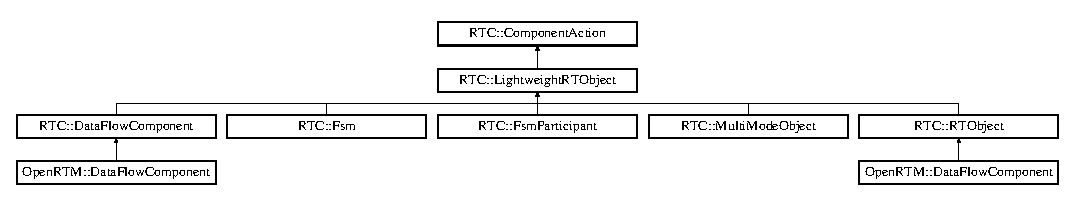
\includegraphics[height=2.25126cm]{interfaceRTC_1_1ComponentAction}
\end{center}
\end{figure}
\subsection*{Public メソッド}
\begin{DoxyCompactItemize}
\item 
{\bf ReturnCode\_\-t} {\bf on\_\-initialize} ()
\item 
{\bf ReturnCode\_\-t} {\bf on\_\-finalize} ()
\item 
{\bf ReturnCode\_\-t} {\bf on\_\-startup} (in {\bf ExecutionContextHandle\_\-t} exec\_\-handle)
\item 
{\bf ReturnCode\_\-t} {\bf on\_\-shutdown} (in {\bf ExecutionContextHandle\_\-t} exec\_\-handle)
\item 
{\bf ReturnCode\_\-t} {\bf on\_\-activated} (in {\bf ExecutionContextHandle\_\-t} exec\_\-handle)
\item 
{\bf ReturnCode\_\-t} {\bf on\_\-deactivated} (in {\bf ExecutionContextHandle\_\-t} exec\_\-handle)
\item 
{\bf ReturnCode\_\-t} {\bf on\_\-aborting} (in {\bf ExecutionContextHandle\_\-t} exec\_\-handle)
\item 
{\bf ReturnCode\_\-t} {\bf on\_\-error} (in {\bf ExecutionContextHandle\_\-t} exec\_\-handle)
\item 
{\bf ReturnCode\_\-t} {\bf on\_\-reset} (in {\bf ExecutionContextHandle\_\-t} exec\_\-handle)
\end{DoxyCompactItemize}


\subsection{関数}
\index{RTC::ComponentAction@{RTC::ComponentAction}!on\_\-aborting@{on\_\-aborting}}
\index{on\_\-aborting@{on\_\-aborting}!RTC::ComponentAction@{RTC::ComponentAction}}
\subsubsection[{on\_\-aborting}]{\setlength{\rightskip}{0pt plus 5cm}{\bf ReturnCode\_\-t} RTC::ComponentAction::on\_\-aborting (in {\bf ExecutionContextHandle\_\-t} {\em exec\_\-handle})}\label{interfaceRTC_1_1ComponentAction_a876e58ebcea16c307e131b3e6a58ddbe}
\index{RTC::ComponentAction@{RTC::ComponentAction}!on\_\-activated@{on\_\-activated}}
\index{on\_\-activated@{on\_\-activated}!RTC::ComponentAction@{RTC::ComponentAction}}
\subsubsection[{on\_\-activated}]{\setlength{\rightskip}{0pt plus 5cm}{\bf ReturnCode\_\-t} RTC::ComponentAction::on\_\-activated (in {\bf ExecutionContextHandle\_\-t} {\em exec\_\-handle})}\label{interfaceRTC_1_1ComponentAction_a4f51f627067d0c54e89c4c0827fa6432}
\index{RTC::ComponentAction@{RTC::ComponentAction}!on\_\-deactivated@{on\_\-deactivated}}
\index{on\_\-deactivated@{on\_\-deactivated}!RTC::ComponentAction@{RTC::ComponentAction}}
\subsubsection[{on\_\-deactivated}]{\setlength{\rightskip}{0pt plus 5cm}{\bf ReturnCode\_\-t} RTC::ComponentAction::on\_\-deactivated (in {\bf ExecutionContextHandle\_\-t} {\em exec\_\-handle})}\label{interfaceRTC_1_1ComponentAction_aa5f9cfb9677ba685be333ad666c87f88}
\index{RTC::ComponentAction@{RTC::ComponentAction}!on\_\-error@{on\_\-error}}
\index{on\_\-error@{on\_\-error}!RTC::ComponentAction@{RTC::ComponentAction}}
\subsubsection[{on\_\-error}]{\setlength{\rightskip}{0pt plus 5cm}{\bf ReturnCode\_\-t} RTC::ComponentAction::on\_\-error (in {\bf ExecutionContextHandle\_\-t} {\em exec\_\-handle})}\label{interfaceRTC_1_1ComponentAction_a110fdde803e9b13f27308b897439962a}
\index{RTC::ComponentAction@{RTC::ComponentAction}!on\_\-finalize@{on\_\-finalize}}
\index{on\_\-finalize@{on\_\-finalize}!RTC::ComponentAction@{RTC::ComponentAction}}
\subsubsection[{on\_\-finalize}]{\setlength{\rightskip}{0pt plus 5cm}{\bf ReturnCode\_\-t} RTC::ComponentAction::on\_\-finalize ()}\label{interfaceRTC_1_1ComponentAction_a9c9e2d638cd2b748609be8a23410aedc}
\index{RTC::ComponentAction@{RTC::ComponentAction}!on\_\-initialize@{on\_\-initialize}}
\index{on\_\-initialize@{on\_\-initialize}!RTC::ComponentAction@{RTC::ComponentAction}}
\subsubsection[{on\_\-initialize}]{\setlength{\rightskip}{0pt plus 5cm}{\bf ReturnCode\_\-t} RTC::ComponentAction::on\_\-initialize ()}\label{interfaceRTC_1_1ComponentAction_a8703b183bc1bed9e2fd3ecac126cb231}
\index{RTC::ComponentAction@{RTC::ComponentAction}!on\_\-reset@{on\_\-reset}}
\index{on\_\-reset@{on\_\-reset}!RTC::ComponentAction@{RTC::ComponentAction}}
\subsubsection[{on\_\-reset}]{\setlength{\rightskip}{0pt plus 5cm}{\bf ReturnCode\_\-t} RTC::ComponentAction::on\_\-reset (in {\bf ExecutionContextHandle\_\-t} {\em exec\_\-handle})}\label{interfaceRTC_1_1ComponentAction_adb0e61bff251337d79c7c7d050d8304e}
\index{RTC::ComponentAction@{RTC::ComponentAction}!on\_\-shutdown@{on\_\-shutdown}}
\index{on\_\-shutdown@{on\_\-shutdown}!RTC::ComponentAction@{RTC::ComponentAction}}
\subsubsection[{on\_\-shutdown}]{\setlength{\rightskip}{0pt plus 5cm}{\bf ReturnCode\_\-t} RTC::ComponentAction::on\_\-shutdown (in {\bf ExecutionContextHandle\_\-t} {\em exec\_\-handle})}\label{interfaceRTC_1_1ComponentAction_accc47711344c811c9bdba0d66a3048f2}
\index{RTC::ComponentAction@{RTC::ComponentAction}!on\_\-startup@{on\_\-startup}}
\index{on\_\-startup@{on\_\-startup}!RTC::ComponentAction@{RTC::ComponentAction}}
\subsubsection[{on\_\-startup}]{\setlength{\rightskip}{0pt plus 5cm}{\bf ReturnCode\_\-t} RTC::ComponentAction::on\_\-startup (in {\bf ExecutionContextHandle\_\-t} {\em exec\_\-handle})}\label{interfaceRTC_1_1ComponentAction_ac305f00c92f4650cf4fc798aac37eef2}


このインタフェースの説明は次のファイルから生成されました:\begin{DoxyCompactItemize}
\item 
{\bf RTC.idl}\end{DoxyCompactItemize}

\section{RTC::ComponentProfile Struct Reference}
\label{structRTC_1_1ComponentProfile}\index{RTC::ComponentProfile@{RTC::ComponentProfile}}


\doxyref{ComponentProfile}{p.}{structRTC_1_1ComponentProfile}.  




{\ttfamily import \char`\"{}RTC.idl\char`\"{};}

\subsection*{Public Attributes}
\begin{DoxyCompactItemize}
\item 
string {\bf instance\_\-name}
\begin{DoxyCompactList}\small\item\em instance\_\-name \item\end{DoxyCompactList}\item 
string {\bf type\_\-name}
\begin{DoxyCompactList}\small\item\em type\_\-name \item\end{DoxyCompactList}\item 
string {\bf description}
\begin{DoxyCompactList}\small\item\em description \item\end{DoxyCompactList}\item 
string {\bf version}
\begin{DoxyCompactList}\small\item\em version \item\end{DoxyCompactList}\item 
string {\bf vendor}
\begin{DoxyCompactList}\small\item\em vendor \item\end{DoxyCompactList}\item 
string {\bf category}
\begin{DoxyCompactList}\small\item\em category \item\end{DoxyCompactList}\item 
{\bf PortProfileList} {\bf port\_\-profiles}
\begin{DoxyCompactList}\small\item\em port\_\-profiles \item\end{DoxyCompactList}\item 
{\bf RTObject} {\bf parent}
\begin{DoxyCompactList}\small\item\em parent \item\end{DoxyCompactList}\item 
{\bf NVList} {\bf properties}
\begin{DoxyCompactList}\small\item\em properties \item\end{DoxyCompactList}\end{DoxyCompactItemize}


\subsection{Detailed Description}
\doxyref{ComponentProfile}{p.}{structRTC_1_1ComponentProfile}. \subsection{Description}\label{namespaceRTC_Description}
\doxyref{ComponentProfile}{p.}{structRTC_1_1ComponentProfile} represents the static state of an \doxyref{RTC}{p.}{namespaceRTC} that is referred to here as the \char`\"{}target\char`\"{} \doxyref{RTC}{p.}{namespaceRTC}. 

\subsection{Member Data Documentation}
\index{RTC::ComponentProfile@{RTC::ComponentProfile}!category@{category}}
\index{category@{category}!RTC::ComponentProfile@{RTC::ComponentProfile}}
\subsubsection[{category}]{\setlength{\rightskip}{0pt plus 5cm}string {\bf RTC::ComponentProfile::category}}\label{structRTC_1_1ComponentProfile_ac79fc17eb8db9fd42ed8e5f84f9171be}


category 

\subsection{Description}\label{namespaceRTC_Description}
This attribute contains the name of a \char`\"{}category\char`\"{} or group to which the target \doxyref{RTC}{p.}{namespaceRTC} belongs. \index{RTC::ComponentProfile@{RTC::ComponentProfile}!description@{description}}
\index{description@{description}!RTC::ComponentProfile@{RTC::ComponentProfile}}
\subsubsection[{description}]{\setlength{\rightskip}{0pt plus 5cm}string {\bf RTC::ComponentProfile::description}}\label{structRTC_1_1ComponentProfile_a874f3699d88630b493e81409071fc119}


description 

\subsection{Description}\label{namespaceRTC_Description}
This attribute shall briefly describe the target \doxyref{RTC}{p.}{namespaceRTC} for the benefit of a human operator. \index{RTC::ComponentProfile@{RTC::ComponentProfile}!instance\_\-name@{instance\_\-name}}
\index{instance\_\-name@{instance\_\-name}!RTC::ComponentProfile@{RTC::ComponentProfile}}
\subsubsection[{instance\_\-name}]{\setlength{\rightskip}{0pt plus 5cm}string {\bf RTC::ComponentProfile::instance\_\-name}}\label{structRTC_1_1ComponentProfile_a52fa51e07ac15e9d35b13ddb227fe991}


instance\_\-name 

\subsection{Description}\label{namespaceRTC_Description}
This attribute shall contain the name of the target \doxyref{RTC}{p.}{namespaceRTC} instance.\subsection{Semantics}\label{namespaceRTC_Semantics}
The instance\_\-name should be unique among \doxyref{RTC}{p.}{namespaceRTC} instances contained within the same containing component. \index{RTC::ComponentProfile@{RTC::ComponentProfile}!parent@{parent}}
\index{parent@{parent}!RTC::ComponentProfile@{RTC::ComponentProfile}}
\subsubsection[{parent}]{\setlength{\rightskip}{0pt plus 5cm}{\bf RTObject} {\bf RTC::ComponentProfile::parent}}\label{structRTC_1_1ComponentProfile_aad7ac4df3d915687a69409be951d1907}


parent 

\subsection{Description}\label{namespaceRTC_Description}
This attribute contains a reference to the \doxyref{RTC}{p.}{namespaceRTC} that contains the target \doxyref{RTC}{p.}{namespaceRTC} instance. If the target \doxyref{RTC}{p.}{namespaceRTC} instance is not owned by any other \doxyref{RTC}{p.}{namespaceRTC}, this field stores a nil reference. \index{RTC::ComponentProfile@{RTC::ComponentProfile}!port\_\-profiles@{port\_\-profiles}}
\index{port\_\-profiles@{port\_\-profiles}!RTC::ComponentProfile@{RTC::ComponentProfile}}
\subsubsection[{port\_\-profiles}]{\setlength{\rightskip}{0pt plus 5cm}{\bf PortProfileList} {\bf RTC::ComponentProfile::port\_\-profiles}}\label{structRTC_1_1ComponentProfile_ade5f8ab4b6048f3e924f404e9937404c}


port\_\-profiles 

\subsection{Description}\label{namespaceRTC_Description}
This attribute contains a list of PortProfiles that describe the ports of the target \doxyref{RTC}{p.}{namespaceRTC}.\subsection{Semantics}\label{namespaceRTC_Semantics}
There shall be a one-\/to-\/one correspondence between the members of this list and the ports of the target \doxyref{RTC}{p.}{namespaceRTC}. \index{RTC::ComponentProfile@{RTC::ComponentProfile}!properties@{properties}}
\index{properties@{properties}!RTC::ComponentProfile@{RTC::ComponentProfile}}
\subsubsection[{properties}]{\setlength{\rightskip}{0pt plus 5cm}{\bf NVList} {\bf RTC::ComponentProfile::properties}}\label{structRTC_1_1ComponentProfile_a5403556c149d6540bd168ae33451d7d1}


properties 

\subsection{Description}\label{namespaceRTC_Description}
This attribute contains additional properties of the target \doxyref{RTC}{p.}{namespaceRTC}.\subsection{Semantics}\label{namespaceRTC_Semantics}
This attribute provides implementations the opportunity to describe additional characteristics of a particular \doxyref{RTC}{p.}{namespaceRTC} that are otherwise outside of the scope of this specification. \index{RTC::ComponentProfile@{RTC::ComponentProfile}!type\_\-name@{type\_\-name}}
\index{type\_\-name@{type\_\-name}!RTC::ComponentProfile@{RTC::ComponentProfile}}
\subsubsection[{type\_\-name}]{\setlength{\rightskip}{0pt plus 5cm}string {\bf RTC::ComponentProfile::type\_\-name}}\label{structRTC_1_1ComponentProfile_a1b44c935bf684d94ecd7866074025213}


type\_\-name 

\subsection{Description}\label{namespaceRTC_Description}
This attribute shall contain the name of the target \doxyref{RTC}{p.}{namespaceRTC} class.\subsection{Semantics}\label{namespaceRTC_Semantics}
Each \doxyref{RTC}{p.}{namespaceRTC} class must have a name that is unique within an application. \index{RTC::ComponentProfile@{RTC::ComponentProfile}!vendor@{vendor}}
\index{vendor@{vendor}!RTC::ComponentProfile@{RTC::ComponentProfile}}
\subsubsection[{vendor}]{\setlength{\rightskip}{0pt plus 5cm}string {\bf RTC::ComponentProfile::vendor}}\label{structRTC_1_1ComponentProfile_a681e9805c9ebbe5b380991aa50841b0f}


vendor 

\subsection{Description}\label{namespaceRTC_Description}
The name of the individual or organization that produced the target \doxyref{RTC}{p.}{namespaceRTC} class. \index{RTC::ComponentProfile@{RTC::ComponentProfile}!version@{version}}
\index{version@{version}!RTC::ComponentProfile@{RTC::ComponentProfile}}
\subsubsection[{version}]{\setlength{\rightskip}{0pt plus 5cm}string {\bf RTC::ComponentProfile::version}}\label{structRTC_1_1ComponentProfile_a3d9684f83c019123418bb644ae23372f}


version 

\subsection{Description}\label{namespaceRTC_Description}
This attribute shall contain the version number of the target \doxyref{RTC}{p.}{namespaceRTC} class.\subsection{Semantics}\label{namespaceRTC_Semantics}
The format of the version number is outside of the scope of this specification. 

The documentation for this struct was generated from the following file:\begin{DoxyCompactItemize}
\item 
{\bf RTC.idl}\end{DoxyCompactItemize}

\section{SDOPackage::Configuration Interface Reference}
\label{interfaceSDOPackage_1_1Configuration}\index{SDOPackage::Configuration@{SDOPackage::Configuration}}


{\ttfamily import \char`\"{}SDOPackage.idl\char`\"{};}

\subsection*{Public Member Functions}
\begin{DoxyCompactItemize}
\item 
boolean {\bf set\_\-device\_\-profile} (in {\bf DeviceProfile} dProfile)  raises (InvalidParameter, NotAvailable, InternalError)
\item 
boolean {\bf add\_\-service\_\-profile} (in {\bf ServiceProfile} sProfile)  raises (InvalidParameter, NotAvailable, InternalError)
\item 
boolean {\bf add\_\-organization} (in {\bf Organization} organization\_\-object)  raises (InvalidParameter, NotAvailable, InternalError)
\item 
boolean {\bf remove\_\-service\_\-profile} (in {\bf UniqueIdentifier} id)  raises (InvalidParameter, NotAvailable, InternalError)
\item 
boolean {\bf remove\_\-organization} (in {\bf UniqueIdentifier} organization\_\-id)  raises (InvalidParameter, NotAvailable, InternalError)
\item 
{\bf ParameterList} {\bf get\_\-configuration\_\-parameters} ()  raises (NotAvailable, InternalError)
\item 
{\bf NVList} {\bf get\_\-configuration\_\-parameter\_\-values} ()  raises (NotAvailable, InternalError)
\item 
any {\bf get\_\-configuration\_\-parameter\_\-value} (in string name)  raises (InvalidParameter, NotAvailable, InternalError)
\item 
boolean {\bf set\_\-configuration\_\-parameter} (in string name, in any value)  raises (InvalidParameter, NotAvailable, InternalError)
\item 
{\bf ConfigurationSetList} {\bf get\_\-configuration\_\-sets} ()  raises (NotAvailable, InternalError)
\item 
{\bf ConfigurationSet} {\bf get\_\-configuration\_\-set} (in {\bf UniqueIdentifier} config\_\-id)  raises (NotAvailable, InternalError)
\item 
boolean {\bf set\_\-configuration\_\-set\_\-values} (in {\bf ConfigurationSet} configuration\_\-set)  raises (InvalidParameter, NotAvailable, InternalError)
\item 
{\bf ConfigurationSet} {\bf get\_\-active\_\-configuration\_\-set} ()  raises (NotAvailable, InternalError)
\item 
boolean {\bf add\_\-configuration\_\-set} (in {\bf ConfigurationSet} configuration\_\-set)  raises (InvalidParameter, NotAvailable, InternalError)
\item 
boolean {\bf remove\_\-configuration\_\-set} (in {\bf UniqueIdentifier} config\_\-id)  raises (InvalidParameter, NotAvailable, InternalError)
\item 
boolean {\bf activate\_\-configuration\_\-set} (in {\bf UniqueIdentifier} config\_\-id)  raises (InvalidParameter, NotAvailable, InternalError)
\end{DoxyCompactItemize}


\subsection{Member Function Documentation}
\index{SDOPackage::Configuration@{SDOPackage::Configuration}!activate\_\-configuration\_\-set@{activate\_\-configuration\_\-set}}
\index{activate\_\-configuration\_\-set@{activate\_\-configuration\_\-set}!SDOPackage::Configuration@{SDOPackage::Configuration}}
\subsubsection[{activate\_\-configuration\_\-set}]{\setlength{\rightskip}{0pt plus 5cm}boolean SDOPackage::Configuration::activate\_\-configuration\_\-set (in {\bf UniqueIdentifier} {\em config\_\-id})  raises (InvalidParameter, NotAvailable, InternalError)}\label{interfaceSDOPackage_1_1Configuration_a328e38e1fa5acd4fb27b1a99912a4923}
\index{SDOPackage::Configuration@{SDOPackage::Configuration}!add\_\-configuration\_\-set@{add\_\-configuration\_\-set}}
\index{add\_\-configuration\_\-set@{add\_\-configuration\_\-set}!SDOPackage::Configuration@{SDOPackage::Configuration}}
\subsubsection[{add\_\-configuration\_\-set}]{\setlength{\rightskip}{0pt plus 5cm}boolean SDOPackage::Configuration::add\_\-configuration\_\-set (in {\bf ConfigurationSet} {\em configuration\_\-set})  raises (InvalidParameter, NotAvailable, InternalError)}\label{interfaceSDOPackage_1_1Configuration_a04a066acc0585d940c058a6fc34f5023}
\index{SDOPackage::Configuration@{SDOPackage::Configuration}!add\_\-organization@{add\_\-organization}}
\index{add\_\-organization@{add\_\-organization}!SDOPackage::Configuration@{SDOPackage::Configuration}}
\subsubsection[{add\_\-organization}]{\setlength{\rightskip}{0pt plus 5cm}boolean SDOPackage::Configuration::add\_\-organization (in {\bf Organization} {\em organization\_\-object})  raises (InvalidParameter, NotAvailable, InternalError)}\label{interfaceSDOPackage_1_1Configuration_ac29fc4106db1df64eb105aa38604b738}
\index{SDOPackage::Configuration@{SDOPackage::Configuration}!add\_\-service\_\-profile@{add\_\-service\_\-profile}}
\index{add\_\-service\_\-profile@{add\_\-service\_\-profile}!SDOPackage::Configuration@{SDOPackage::Configuration}}
\subsubsection[{add\_\-service\_\-profile}]{\setlength{\rightskip}{0pt plus 5cm}boolean SDOPackage::Configuration::add\_\-service\_\-profile (in {\bf ServiceProfile} {\em sProfile})  raises (InvalidParameter, NotAvailable, InternalError)}\label{interfaceSDOPackage_1_1Configuration_a406b04eabcfed65c4f9b0396a89ccc4d}
\index{SDOPackage::Configuration@{SDOPackage::Configuration}!get\_\-active\_\-configuration\_\-set@{get\_\-active\_\-configuration\_\-set}}
\index{get\_\-active\_\-configuration\_\-set@{get\_\-active\_\-configuration\_\-set}!SDOPackage::Configuration@{SDOPackage::Configuration}}
\subsubsection[{get\_\-active\_\-configuration\_\-set}]{\setlength{\rightskip}{0pt plus 5cm}{\bf ConfigurationSet} SDOPackage::Configuration::get\_\-active\_\-configuration\_\-set ()  raises (NotAvailable, InternalError)}\label{interfaceSDOPackage_1_1Configuration_a7f89d399b04ce71804c27c623df61cbc}
\index{SDOPackage::Configuration@{SDOPackage::Configuration}!get\_\-configuration\_\-parameter\_\-value@{get\_\-configuration\_\-parameter\_\-value}}
\index{get\_\-configuration\_\-parameter\_\-value@{get\_\-configuration\_\-parameter\_\-value}!SDOPackage::Configuration@{SDOPackage::Configuration}}
\subsubsection[{get\_\-configuration\_\-parameter\_\-value}]{\setlength{\rightskip}{0pt plus 5cm}any SDOPackage::Configuration::get\_\-configuration\_\-parameter\_\-value (in string {\em name})  raises (InvalidParameter, NotAvailable, InternalError)}\label{interfaceSDOPackage_1_1Configuration_affd15445c9c4b0ea3a510a9551c29409}
\index{SDOPackage::Configuration@{SDOPackage::Configuration}!get\_\-configuration\_\-parameter\_\-values@{get\_\-configuration\_\-parameter\_\-values}}
\index{get\_\-configuration\_\-parameter\_\-values@{get\_\-configuration\_\-parameter\_\-values}!SDOPackage::Configuration@{SDOPackage::Configuration}}
\subsubsection[{get\_\-configuration\_\-parameter\_\-values}]{\setlength{\rightskip}{0pt plus 5cm}{\bf NVList} SDOPackage::Configuration::get\_\-configuration\_\-parameter\_\-values ()  raises (NotAvailable, InternalError)}\label{interfaceSDOPackage_1_1Configuration_ac59b71044e697ae6d7184437340ccff2}
\index{SDOPackage::Configuration@{SDOPackage::Configuration}!get\_\-configuration\_\-parameters@{get\_\-configuration\_\-parameters}}
\index{get\_\-configuration\_\-parameters@{get\_\-configuration\_\-parameters}!SDOPackage::Configuration@{SDOPackage::Configuration}}
\subsubsection[{get\_\-configuration\_\-parameters}]{\setlength{\rightskip}{0pt plus 5cm}{\bf ParameterList} SDOPackage::Configuration::get\_\-configuration\_\-parameters ()  raises (NotAvailable, InternalError)}\label{interfaceSDOPackage_1_1Configuration_a8b0db85c0fb5ed92c1664686f649298c}
\index{SDOPackage::Configuration@{SDOPackage::Configuration}!get\_\-configuration\_\-set@{get\_\-configuration\_\-set}}
\index{get\_\-configuration\_\-set@{get\_\-configuration\_\-set}!SDOPackage::Configuration@{SDOPackage::Configuration}}
\subsubsection[{get\_\-configuration\_\-set}]{\setlength{\rightskip}{0pt plus 5cm}{\bf ConfigurationSet} SDOPackage::Configuration::get\_\-configuration\_\-set (in {\bf UniqueIdentifier} {\em config\_\-id})  raises (NotAvailable, InternalError)}\label{interfaceSDOPackage_1_1Configuration_af41445e0bcc9ea6241f77d3f687ad535}
\index{SDOPackage::Configuration@{SDOPackage::Configuration}!get\_\-configuration\_\-sets@{get\_\-configuration\_\-sets}}
\index{get\_\-configuration\_\-sets@{get\_\-configuration\_\-sets}!SDOPackage::Configuration@{SDOPackage::Configuration}}
\subsubsection[{get\_\-configuration\_\-sets}]{\setlength{\rightskip}{0pt plus 5cm}{\bf ConfigurationSetList} SDOPackage::Configuration::get\_\-configuration\_\-sets ()  raises (NotAvailable, InternalError)}\label{interfaceSDOPackage_1_1Configuration_aca0fc0ab3c00a1c386883be766f77a9e}
\index{SDOPackage::Configuration@{SDOPackage::Configuration}!remove\_\-configuration\_\-set@{remove\_\-configuration\_\-set}}
\index{remove\_\-configuration\_\-set@{remove\_\-configuration\_\-set}!SDOPackage::Configuration@{SDOPackage::Configuration}}
\subsubsection[{remove\_\-configuration\_\-set}]{\setlength{\rightskip}{0pt plus 5cm}boolean SDOPackage::Configuration::remove\_\-configuration\_\-set (in {\bf UniqueIdentifier} {\em config\_\-id})  raises (InvalidParameter, NotAvailable, InternalError)}\label{interfaceSDOPackage_1_1Configuration_a2b8fee9e3106cb08c72590f3716d809e}
\index{SDOPackage::Configuration@{SDOPackage::Configuration}!remove\_\-organization@{remove\_\-organization}}
\index{remove\_\-organization@{remove\_\-organization}!SDOPackage::Configuration@{SDOPackage::Configuration}}
\subsubsection[{remove\_\-organization}]{\setlength{\rightskip}{0pt plus 5cm}boolean SDOPackage::Configuration::remove\_\-organization (in {\bf UniqueIdentifier} {\em organization\_\-id})  raises (InvalidParameter, NotAvailable, InternalError)}\label{interfaceSDOPackage_1_1Configuration_a3b891d4f199c83a774643beda3a25d76}
\index{SDOPackage::Configuration@{SDOPackage::Configuration}!remove\_\-service\_\-profile@{remove\_\-service\_\-profile}}
\index{remove\_\-service\_\-profile@{remove\_\-service\_\-profile}!SDOPackage::Configuration@{SDOPackage::Configuration}}
\subsubsection[{remove\_\-service\_\-profile}]{\setlength{\rightskip}{0pt plus 5cm}boolean SDOPackage::Configuration::remove\_\-service\_\-profile (in {\bf UniqueIdentifier} {\em id})  raises (InvalidParameter, NotAvailable, InternalError)}\label{interfaceSDOPackage_1_1Configuration_a9d80d9a2a1ab5cb4bfa670d8b648e3fc}
\index{SDOPackage::Configuration@{SDOPackage::Configuration}!set\_\-configuration\_\-parameter@{set\_\-configuration\_\-parameter}}
\index{set\_\-configuration\_\-parameter@{set\_\-configuration\_\-parameter}!SDOPackage::Configuration@{SDOPackage::Configuration}}
\subsubsection[{set\_\-configuration\_\-parameter}]{\setlength{\rightskip}{0pt plus 5cm}boolean SDOPackage::Configuration::set\_\-configuration\_\-parameter (in string {\em name}, \/  in any {\em value})  raises (InvalidParameter, NotAvailable, InternalError)}\label{interfaceSDOPackage_1_1Configuration_ae9314a2cc5743932d9cc44c41393bf35}
\index{SDOPackage::Configuration@{SDOPackage::Configuration}!set\_\-configuration\_\-set\_\-values@{set\_\-configuration\_\-set\_\-values}}
\index{set\_\-configuration\_\-set\_\-values@{set\_\-configuration\_\-set\_\-values}!SDOPackage::Configuration@{SDOPackage::Configuration}}
\subsubsection[{set\_\-configuration\_\-set\_\-values}]{\setlength{\rightskip}{0pt plus 5cm}boolean SDOPackage::Configuration::set\_\-configuration\_\-set\_\-values (in {\bf ConfigurationSet} {\em configuration\_\-set})  raises (InvalidParameter, NotAvailable, InternalError)}\label{interfaceSDOPackage_1_1Configuration_a82d62dcfce26a9cf41bfa79a26a79fa5}
\index{SDOPackage::Configuration@{SDOPackage::Configuration}!set\_\-device\_\-profile@{set\_\-device\_\-profile}}
\index{set\_\-device\_\-profile@{set\_\-device\_\-profile}!SDOPackage::Configuration@{SDOPackage::Configuration}}
\subsubsection[{set\_\-device\_\-profile}]{\setlength{\rightskip}{0pt plus 5cm}boolean SDOPackage::Configuration::set\_\-device\_\-profile (in {\bf DeviceProfile} {\em dProfile})  raises (InvalidParameter, NotAvailable, InternalError)}\label{interfaceSDOPackage_1_1Configuration_a9bc9b647255e601b692eed2410e43927}


The documentation for this interface was generated from the following file:\begin{DoxyCompactItemize}
\item 
{\bf SDOPackage.idl}\end{DoxyCompactItemize}

\section{構造体 SDOPackage::ConfigurationSet}
\label{structSDOPackage_1_1ConfigurationSet}\index{SDOPackage::ConfigurationSet@{SDOPackage::ConfigurationSet}}


{\ttfamily import \char`\"{}SDOPackage.idl\char`\"{};}

\subsection*{Public 変数}
\begin{DoxyCompactItemize}
\item 
string {\bf id}
\item 
string {\bf description}
\item 
{\bf NVList} {\bf configuration\_\-data}
\end{DoxyCompactItemize}


\subsection{変数}
\index{SDOPackage::ConfigurationSet@{SDOPackage::ConfigurationSet}!configuration\_\-data@{configuration\_\-data}}
\index{configuration\_\-data@{configuration\_\-data}!SDOPackage::ConfigurationSet@{SDOPackage::ConfigurationSet}}
\subsubsection[{configuration\_\-data}]{\setlength{\rightskip}{0pt plus 5cm}{\bf NVList} {\bf SDOPackage::ConfigurationSet::configuration\_\-data}}\label{structSDOPackage_1_1ConfigurationSet_ae28985bc93cdf23fc12357aa03552ebb}
\index{SDOPackage::ConfigurationSet@{SDOPackage::ConfigurationSet}!description@{description}}
\index{description@{description}!SDOPackage::ConfigurationSet@{SDOPackage::ConfigurationSet}}
\subsubsection[{description}]{\setlength{\rightskip}{0pt plus 5cm}string {\bf SDOPackage::ConfigurationSet::description}}\label{structSDOPackage_1_1ConfigurationSet_ab29b970de7ba627ab35ad294e92c7983}
\index{SDOPackage::ConfigurationSet@{SDOPackage::ConfigurationSet}!id@{id}}
\index{id@{id}!SDOPackage::ConfigurationSet@{SDOPackage::ConfigurationSet}}
\subsubsection[{id}]{\setlength{\rightskip}{0pt plus 5cm}string {\bf SDOPackage::ConfigurationSet::id}}\label{structSDOPackage_1_1ConfigurationSet_a2e6620e0ecf1dbbefb4d25ec3d0e6ca5}


この構造体の説明は次のファイルから生成されました:\begin{DoxyCompactItemize}
\item 
{\bf SDOPackage.idl}\end{DoxyCompactItemize}

\section{RTC::ConnectorProfile Struct Reference}
\label{structRTC_1_1ConnectorProfile}\index{RTC::ConnectorProfile@{RTC::ConnectorProfile}}


\doxyref{ConnectorProfile}{p.}{structRTC_1_1ConnectorProfile}.  




{\ttfamily import \char`\"{}RTC.idl\char`\"{};}

\subsection*{Public Attributes}
\begin{DoxyCompactItemize}
\item 
string {\bf name}
\begin{DoxyCompactList}\small\item\em name \item\end{DoxyCompactList}\item 
{\bf UniqueIdentifier} {\bf connector\_\-id}
\begin{DoxyCompactList}\small\item\em connector\_\-id \item\end{DoxyCompactList}\item 
{\bf PortServiceList} {\bf ports}
\begin{DoxyCompactList}\small\item\em ports \item\end{DoxyCompactList}\item 
{\bf NVList} {\bf properties}
\begin{DoxyCompactList}\small\item\em properties \item\end{DoxyCompactList}\end{DoxyCompactItemize}


\subsection{Detailed Description}
\doxyref{ConnectorProfile}{p.}{structRTC_1_1ConnectorProfile}. \subsection{Description}\label{namespaceRTC_Description}
The \doxyref{ConnectorProfile}{p.}{structRTC_1_1ConnectorProfile} contains information about a connection between the ports of collaborating RTCs. 

\subsection{Member Data Documentation}
\index{RTC::ConnectorProfile@{RTC::ConnectorProfile}!connector\_\-id@{connector\_\-id}}
\index{connector\_\-id@{connector\_\-id}!RTC::ConnectorProfile@{RTC::ConnectorProfile}}
\subsubsection[{connector\_\-id}]{\setlength{\rightskip}{0pt plus 5cm}{\bf UniqueIdentifier} {\bf RTC::ConnectorProfile::connector\_\-id}}\label{structRTC_1_1ConnectorProfile_a35ab0f337d42a13f145884b8d1fb0ceb}


connector\_\-id 

\subsection{Description}\label{namespaceRTC_Description}
Each connector has a unique identifier that is assigned when connection is established. This attribute stores that identifier. \index{RTC::ConnectorProfile@{RTC::ConnectorProfile}!name@{name}}
\index{name@{name}!RTC::ConnectorProfile@{RTC::ConnectorProfile}}
\subsubsection[{name}]{\setlength{\rightskip}{0pt plus 5cm}string {\bf RTC::ConnectorProfile::name}}\label{structRTC_1_1ConnectorProfile_a7388e47fe2c24d93b0f583cb13a18b52}


name 

\subsection{Description}\label{namespaceRTC_Description}
This attribute contains the name of this connection. \index{RTC::ConnectorProfile@{RTC::ConnectorProfile}!ports@{ports}}
\index{ports@{ports}!RTC::ConnectorProfile@{RTC::ConnectorProfile}}
\subsubsection[{ports}]{\setlength{\rightskip}{0pt plus 5cm}{\bf PortServiceList} {\bf RTC::ConnectorProfile::ports}}\label{structRTC_1_1ConnectorProfile_a84117d3a0082f25b2846a35c23cf54ac}


ports 

\subsection{Description}\label{namespaceRTC_Description}
This field stores references to all ports connected by the target connector. \index{RTC::ConnectorProfile@{RTC::ConnectorProfile}!properties@{properties}}
\index{properties@{properties}!RTC::ConnectorProfile@{RTC::ConnectorProfile}}
\subsubsection[{properties}]{\setlength{\rightskip}{0pt plus 5cm}{\bf NVList} {\bf RTC::ConnectorProfile::properties}}\label{structRTC_1_1ConnectorProfile_a7968dd3b23e93c8c5af7b2762bbd4e80}


properties 

\subsection{Description}\label{namespaceRTC_Description}
This attribute contains additional properties of the connection.\subsection{Semantics}\label{namespaceRTC_Semantics}
This attribute provides implementations the opportunity to describe additional characteristics of a particular connection that are outside of the scope of this specification. 

The documentation for this struct was generated from the following file:\begin{DoxyCompactItemize}
\item 
{\bf RTC.idl}\end{DoxyCompactItemize}

\section{RTC::DataFlowComponent Interface Reference}
\label{interfaceRTC_1_1DataFlowComponent}\index{RTC::DataFlowComponent@{RTC::DataFlowComponent}}


dataFlowComponent  




{\ttfamily import \char`\"{}RTC.idl\char`\"{};}

Inheritance diagram for RTC::DataFlowComponent:\begin{figure}[H]
\begin{center}
\leavevmode
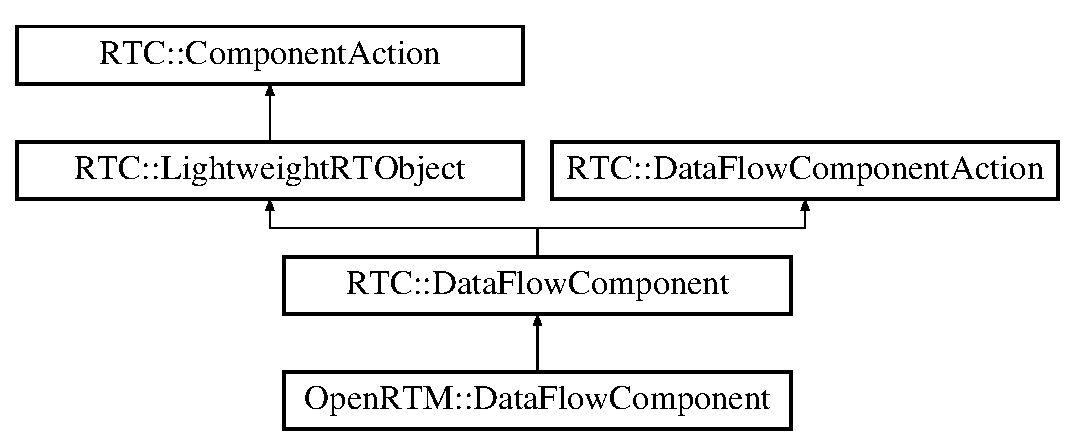
\includegraphics[height=4cm]{interfaceRTC_1_1DataFlowComponent}
\end{center}
\end{figure}
\subsection*{Public Member Functions}
\begin{DoxyCompactItemize}
\item 
{\bf ReturnCode\_\-t} {\bf initialize} ()
\begin{DoxyCompactList}\small\item\em initialize \item\end{DoxyCompactList}\item 
{\bf ReturnCode\_\-t} {\bf finalize} ()
\begin{DoxyCompactList}\small\item\em finalize \item\end{DoxyCompactList}\item 
boolean {\bf is\_\-alive} (in {\bf ExecutionContext} exec\_\-context)
\begin{DoxyCompactList}\small\item\em is\_\-alive \item\end{DoxyCompactList}\item 
{\bf ReturnCode\_\-t} {\bf exit} ()
\begin{DoxyCompactList}\small\item\em exit \item\end{DoxyCompactList}\item 
{\bf ExecutionContextHandle\_\-t} {\bf attach\_\-context} (in {\bf ExecutionContext} exec\_\-context)
\begin{DoxyCompactList}\small\item\em attach\_\-context \item\end{DoxyCompactList}\item 
{\bf ReturnCode\_\-t} {\bf detach\_\-context} (in {\bf ExecutionContextHandle\_\-t} exec\_\-handle)
\begin{DoxyCompactList}\small\item\em detach\_\-context \item\end{DoxyCompactList}\item 
{\bf ExecutionContext} {\bf get\_\-context} (in {\bf ExecutionContextHandle\_\-t} exec\_\-handle)
\begin{DoxyCompactList}\small\item\em get\_\-context \item\end{DoxyCompactList}\item 
{\bf ExecutionContextList} {\bf get\_\-owned\_\-contexts} ()
\begin{DoxyCompactList}\small\item\em get\_\-owned\_\-contexts \item\end{DoxyCompactList}\item 
{\bf ExecutionContextList} {\bf get\_\-participating\_\-contexts} ()
\begin{DoxyCompactList}\small\item\em $\ast$ get\_\-participating\_\-contexts \item\end{DoxyCompactList}\item 
{\bf ExecutionContextHandle\_\-t} {\bf get\_\-context\_\-handle} (in {\bf ExecutionContext} cxt)
\begin{DoxyCompactList}\small\item\em get\_\-context\_\-handle \item\end{DoxyCompactList}\item 
{\bf ReturnCode\_\-t} {\bf on\_\-initialize} ()
\begin{DoxyCompactList}\small\item\em on\_\-initialize \item\end{DoxyCompactList}\item 
{\bf ReturnCode\_\-t} {\bf on\_\-finalize} ()
\begin{DoxyCompactList}\small\item\em on\_\-finalize \item\end{DoxyCompactList}\item 
{\bf ReturnCode\_\-t} {\bf on\_\-startup} (in {\bf ExecutionContextHandle\_\-t} exec\_\-handle)
\begin{DoxyCompactList}\small\item\em on\_\-startup \item\end{DoxyCompactList}\item 
{\bf ReturnCode\_\-t} {\bf on\_\-shutdown} (in {\bf ExecutionContextHandle\_\-t} exec\_\-handle)
\begin{DoxyCompactList}\small\item\em on\_\-shutdown \item\end{DoxyCompactList}\item 
{\bf ReturnCode\_\-t} {\bf on\_\-activated} (in {\bf ExecutionContextHandle\_\-t} exec\_\-handle)
\begin{DoxyCompactList}\small\item\em on\_\-activated \item\end{DoxyCompactList}\item 
{\bf ReturnCode\_\-t} {\bf on\_\-deactivated} (in {\bf ExecutionContextHandle\_\-t} exec\_\-handle)
\begin{DoxyCompactList}\small\item\em on\_\-deactivated \item\end{DoxyCompactList}\item 
{\bf ReturnCode\_\-t} {\bf on\_\-aborting} (in {\bf ExecutionContextHandle\_\-t} exec\_\-handle)
\begin{DoxyCompactList}\small\item\em on\_\-aborting \item\end{DoxyCompactList}\item 
{\bf ReturnCode\_\-t} {\bf on\_\-error} (in {\bf ExecutionContextHandle\_\-t} exec\_\-handle)
\begin{DoxyCompactList}\small\item\em on\_\-error \item\end{DoxyCompactList}\item 
{\bf ReturnCode\_\-t} {\bf on\_\-reset} (in {\bf ExecutionContextHandle\_\-t} exec\_\-handle)
\begin{DoxyCompactList}\small\item\em on\_\-reset \item\end{DoxyCompactList}\item 
{\bf ReturnCode\_\-t} {\bf on\_\-execute} (in {\bf ExecutionContextHandle\_\-t} exec\_\-handle)
\begin{DoxyCompactList}\small\item\em on\_\-execute \item\end{DoxyCompactList}\item 
{\bf ReturnCode\_\-t} {\bf on\_\-state\_\-update} (in {\bf ExecutionContextHandle\_\-t} exec\_\-handle)
\begin{DoxyCompactList}\small\item\em on\_\-state\_\-update \item\end{DoxyCompactList}\item 
{\bf ReturnCode\_\-t} {\bf on\_\-rate\_\-changed} (in {\bf ExecutionContextHandle\_\-t} exec\_\-handle)
\begin{DoxyCompactList}\small\item\em on\_\-rate\_\-changed \item\end{DoxyCompactList}\end{DoxyCompactItemize}


\subsection{Detailed Description}
dataFlowComponent \subsection{Description}\label{namespaceRTC_Description}
The dataFlowComponent stereotype may be applied to a component type to indicate that its instances should be executed in sorted order by a periodic execution context.\subsection{Constraints}\label{interfaceRTC_1_1LightweightRTObject_Constraints}

\begin{DoxyItemize}
\item An instance of a component extended by the dataFlowComponent stereotype must participate in at least one $\ast$ execution context of kind PERIODIC, which shall also be used for the execution of any contained data flow components.
\end{DoxyItemize}


\begin{DoxyItemize}
\item A component extended by dataFlowComponent must realize the interface \doxyref{DataFlowComponentAction}{p.}{interfaceRTC_1_1DataFlowComponentAction}. 
\end{DoxyItemize}

\subsection{Member Function Documentation}
\index{RTC::DataFlowComponent@{RTC::DataFlowComponent}!attach\_\-context@{attach\_\-context}}
\index{attach\_\-context@{attach\_\-context}!RTC::DataFlowComponent@{RTC::DataFlowComponent}}
\subsubsection[{attach\_\-context}]{\setlength{\rightskip}{0pt plus 5cm}{\bf ExecutionContextHandle\_\-t} RTC::LightweightRTObject::attach\_\-context (in {\bf ExecutionContext} {\em exec\_\-context})\hspace{0.3cm}{\ttfamily  [inherited]}}\label{interfaceRTC_1_1LightweightRTObject_a48dbdbcac3254c29ad01d43a4ee5a00c}


attach\_\-context 

\subsection{Description}\label{namespaceRTC_Description}
Inform this \doxyref{RTC}{p.}{namespaceRTC} that it is participating in the given execution context. Return a handle that represents the association of this \doxyref{RTC}{p.}{namespaceRTC} with the context.\subsection{Semantics}\label{namespaceRTC_Semantics}
This operation is intended to be invoked by ExecutionContextOperations::add\_\-component (see Section 5.2.2.6.6). It is not intended for use by other clients. \index{RTC::DataFlowComponent@{RTC::DataFlowComponent}!detach\_\-context@{detach\_\-context}}
\index{detach\_\-context@{detach\_\-context}!RTC::DataFlowComponent@{RTC::DataFlowComponent}}
\subsubsection[{detach\_\-context}]{\setlength{\rightskip}{0pt plus 5cm}{\bf ReturnCode\_\-t} RTC::LightweightRTObject::detach\_\-context (in {\bf ExecutionContextHandle\_\-t} {\em exec\_\-handle})\hspace{0.3cm}{\ttfamily  [inherited]}}\label{interfaceRTC_1_1LightweightRTObject_a8eb94420ca08e8f7acaa778ed883b9a4}


detach\_\-context 

\subsection{Description}\label{namespaceRTC_Description}
Inform this \doxyref{RTC}{p.}{namespaceRTC} that it is no longer participating in the given execution context.\subsection{Semantics}\label{namespaceRTC_Semantics}
This operation is intended to be invoked by ExecutionContextOperations::remove\_\-component (see Section 5.2.2.6.7). It is not intended for use by other clients.\subsection{Constraints}\label{interfaceRTC_1_1LightweightRTObject_Constraints}

\begin{DoxyItemize}
\item This operation may not be invoked if this \doxyref{RTC}{p.}{namespaceRTC} is not already participating in the execution context. Such a call shall fail with ReturnCode\_\-t::PRECONDITION\_\-NOT\_\-MET.
\end{DoxyItemize}


\begin{DoxyItemize}
\item This operation may not be invoked if this \doxyref{RTC}{p.}{namespaceRTC} is Active in the indicated execution context. Otherwise, it shall fail with ReturnCode\_\-t::PRECONDITION\_\-NOT\_\-MET. 
\end{DoxyItemize}\index{RTC::DataFlowComponent@{RTC::DataFlowComponent}!exit@{exit}}
\index{exit@{exit}!RTC::DataFlowComponent@{RTC::DataFlowComponent}}
\subsubsection[{exit}]{\setlength{\rightskip}{0pt plus 5cm}{\bf ReturnCode\_\-t} RTC::LightweightRTObject::exit ()\hspace{0.3cm}{\ttfamily  [inherited]}}\label{interfaceRTC_1_1LightweightRTObject_a49bd940b6964fa80d696db15b45c2f87}


exit 

\subsection{Description}\label{namespaceRTC_Description}
Stop the RTC��s execution context(s) and finalize it along with its contents.\subsection{Semantics}\label{namespaceRTC_Semantics}
Any execution contexts for which the \doxyref{RTC}{p.}{namespaceRTC} is the owner shall be stopped. If the \doxyref{RTC}{p.}{namespaceRTC} participates in any execution contexts belonging to another \doxyref{RTC}{p.}{namespaceRTC} that contains it, directly or indirectly (i.e., the containing \doxyref{RTC}{p.}{namespaceRTC} is the owner of the \doxyref{ExecutionContext}{p.}{interfaceRTC_1_1ExecutionContext}), it shall be deactivated in those contexts. After the \doxyref{RTC}{p.}{namespaceRTC} is no longer Active in any Running execution context, it and any RTCs contained transitively within it shall be finalized.\subsection{Constraints}\label{interfaceRTC_1_1LightweightRTObject_Constraints}
An \doxyref{RTC}{p.}{namespaceRTC} cannot be exited if it has not yet been initialized. Any attempt to exit an \doxyref{RTC}{p.}{namespaceRTC} that is in the Created state shall fail with ReturnCode\_\-t::PRECONDITION\_\-NOT\_\-MET. \index{RTC::DataFlowComponent@{RTC::DataFlowComponent}!finalize@{finalize}}
\index{finalize@{finalize}!RTC::DataFlowComponent@{RTC::DataFlowComponent}}
\subsubsection[{finalize}]{\setlength{\rightskip}{0pt plus 5cm}{\bf ReturnCode\_\-t} RTC::LightweightRTObject::finalize ()\hspace{0.3cm}{\ttfamily  [inherited]}}\label{interfaceRTC_1_1LightweightRTObject_a23466f177b4289662ea035be831426ad}


finalize 

\subsection{Description}\label{namespaceRTC_Description}
Finalize the \doxyref{RTC}{p.}{namespaceRTC} that realizes this interface, preparing it for destruction.\subsection{Semantics}\label{namespaceRTC_Semantics}
This invocation of this operation shall result in the invocation of the callback \doxyref{ComponentAction::on\_\-finalize}{p.}{interfaceRTC_1_1ComponentAction_a9c9e2d638cd2b748609be8a23410aedc}\subsection{Constraints}\label{interfaceRTC_1_1LightweightRTObject_Constraints}

\begin{DoxyItemize}
\item An \doxyref{RTC}{p.}{namespaceRTC} may not be finalized while it is participating in any execution context. It must first be removed with ExecutionContextOperations::remove\_\-component. Otherwise, this operation shall fail with ReturnCode\_\-t::PRECONDITION\_\-NOT\_\-MET. See Figure 5.9.
\end{DoxyItemize}


\begin{DoxyItemize}
\item An \doxyref{RTC}{p.}{namespaceRTC} may not be finalized while it is in the Created state. Any attempt to invoke this operation while in that state shall fail with ReturnCode\_\-t::PRECONDITION\_\-NOT\_\-MET.
\end{DoxyItemize}


\begin{DoxyItemize}
\item Application developers are not expected to call this operation directly; it exists for use by the \doxyref{RTC}{p.}{namespaceRTC} infrastructure. 
\end{DoxyItemize}\index{RTC::DataFlowComponent@{RTC::DataFlowComponent}!get\_\-context@{get\_\-context}}
\index{get\_\-context@{get\_\-context}!RTC::DataFlowComponent@{RTC::DataFlowComponent}}
\subsubsection[{get\_\-context}]{\setlength{\rightskip}{0pt plus 5cm}{\bf ExecutionContext} RTC::LightweightRTObject::get\_\-context (in {\bf ExecutionContextHandle\_\-t} {\em exec\_\-handle})\hspace{0.3cm}{\ttfamily  [inherited]}}\label{interfaceRTC_1_1LightweightRTObject_a7bb123faf81bcb57542c3a17f10948d6}


get\_\-context 

\subsection{Description}\label{namespaceRTC_Description}
Obtain a reference to the execution context represented by the given handle.\subsection{Semantics}\label{namespaceRTC_Semantics}
The mapping from handle to context is specific to a particular \doxyref{RTC}{p.}{namespaceRTC} instance. The given handle must have been obtained by a previous call to attach\_\-context on this \doxyref{RTC}{p.}{namespaceRTC}. \index{RTC::DataFlowComponent@{RTC::DataFlowComponent}!get\_\-context\_\-handle@{get\_\-context\_\-handle}}
\index{get\_\-context\_\-handle@{get\_\-context\_\-handle}!RTC::DataFlowComponent@{RTC::DataFlowComponent}}
\subsubsection[{get\_\-context\_\-handle}]{\setlength{\rightskip}{0pt plus 5cm}{\bf ExecutionContextHandle\_\-t} RTC::LightweightRTObject::get\_\-context\_\-handle (in {\bf ExecutionContext} {\em cxt})\hspace{0.3cm}{\ttfamily  [inherited]}}\label{interfaceRTC_1_1LightweightRTObject_af54041744c01d68026aa200276e12f45}


get\_\-context\_\-handle 

\subsection{Description}\label{namespaceRTC_Description}
This operation returns a handle that is associated with the given execution context. \index{RTC::DataFlowComponent@{RTC::DataFlowComponent}!get\_\-owned\_\-contexts@{get\_\-owned\_\-contexts}}
\index{get\_\-owned\_\-contexts@{get\_\-owned\_\-contexts}!RTC::DataFlowComponent@{RTC::DataFlowComponent}}
\subsubsection[{get\_\-owned\_\-contexts}]{\setlength{\rightskip}{0pt plus 5cm}{\bf ExecutionContextList} RTC::LightweightRTObject::get\_\-owned\_\-contexts ()\hspace{0.3cm}{\ttfamily  [inherited]}}\label{interfaceRTC_1_1LightweightRTObject_aea9dd2a447cc3ddc55f20aab698da408}


get\_\-owned\_\-contexts 

\subsection{Description}\label{namespaceRTC_Description}
This operation returns a list of all execution contexts owned by this \doxyref{RTC}{p.}{namespaceRTC}. \index{RTC::DataFlowComponent@{RTC::DataFlowComponent}!get\_\-participating\_\-contexts@{get\_\-participating\_\-contexts}}
\index{get\_\-participating\_\-contexts@{get\_\-participating\_\-contexts}!RTC::DataFlowComponent@{RTC::DataFlowComponent}}
\subsubsection[{get\_\-participating\_\-contexts}]{\setlength{\rightskip}{0pt plus 5cm}{\bf ExecutionContextList} RTC::LightweightRTObject::get\_\-participating\_\-contexts ()\hspace{0.3cm}{\ttfamily  [inherited]}}\label{interfaceRTC_1_1LightweightRTObject_af2224880b89275ecf82efad0999b022a}


$\ast$ get\_\-participating\_\-contexts 

\subsection{Description}\label{namespaceRTC_Description}
This operation returns a list of all execution contexts in which this \doxyref{RTC}{p.}{namespaceRTC} participates.\subsection{Semantics}\label{namespaceRTC_Semantics}
Each call to attach\_\-context causes the provided context to be added to this list. Each call to detach\_\-context causes the provided context to be removed from this list. \index{RTC::DataFlowComponent@{RTC::DataFlowComponent}!initialize@{initialize}}
\index{initialize@{initialize}!RTC::DataFlowComponent@{RTC::DataFlowComponent}}
\subsubsection[{initialize}]{\setlength{\rightskip}{0pt plus 5cm}{\bf ReturnCode\_\-t} RTC::LightweightRTObject::initialize ()\hspace{0.3cm}{\ttfamily  [inherited]}}\label{interfaceRTC_1_1LightweightRTObject_afb28c4d97677804da09488578b840eb5}


initialize 

\subsection{Description}\label{namespaceRTC_Description}
Initialize the \doxyref{RTC}{p.}{namespaceRTC} that realizes this interface.\subsection{Semantics}\label{namespaceRTC_Semantics}
The invocation of this operation shall result in the invocation of the callback \doxyref{ComponentAction::on\_\-initialize}{p.}{interfaceRTC_1_1ComponentAction_a8703b183bc1bed9e2fd3ecac126cb231}.\subsection{Constraints}\label{interfaceRTC_1_1LightweightRTObject_Constraints}

\begin{DoxyItemize}
\item An \doxyref{RTC}{p.}{namespaceRTC} may be initialized only while it is in the Created state. Any attempt to invoke this operation while in another state shall fail with ReturnCode\_\-t::PRECONDITION\_\-NOT\_\-MET.
\item Application developers are not expected to call this operation directly; it exists for use by the \doxyref{RTC}{p.}{namespaceRTC} infrastructure. 
\end{DoxyItemize}\index{RTC::DataFlowComponent@{RTC::DataFlowComponent}!is\_\-alive@{is\_\-alive}}
\index{is\_\-alive@{is\_\-alive}!RTC::DataFlowComponent@{RTC::DataFlowComponent}}
\subsubsection[{is\_\-alive}]{\setlength{\rightskip}{0pt plus 5cm}boolean RTC::LightweightRTObject::is\_\-alive (in {\bf ExecutionContext} {\em exec\_\-context})\hspace{0.3cm}{\ttfamily  [inherited]}}\label{interfaceRTC_1_1LightweightRTObject_aa07c8c299b0addc49887508c1ee7be27}


is\_\-alive 

\subsection{Description}\label{namespaceRTC_Description}
A component is alive or not regardless of the execution context from which it is observed. However, whether or not it is Active, Inactive, or in Error is dependent on the execution context(s) (see Figure 5.7) in which it is running. That is, it may be Active in one context but Inactive in another. Therefore, this operation shall report whether this \doxyref{RTC}{p.}{namespaceRTC} is either Active, Inactive, or in Error; which of those states a component is in with respect to a particular context may be queried from the context itself. \index{RTC::DataFlowComponent@{RTC::DataFlowComponent}!on\_\-aborting@{on\_\-aborting}}
\index{on\_\-aborting@{on\_\-aborting}!RTC::DataFlowComponent@{RTC::DataFlowComponent}}
\subsubsection[{on\_\-aborting}]{\setlength{\rightskip}{0pt plus 5cm}{\bf ReturnCode\_\-t} RTC::ComponentAction::on\_\-aborting (in {\bf ExecutionContextHandle\_\-t} {\em exec\_\-handle})\hspace{0.3cm}{\ttfamily  [inherited]}}\label{interfaceRTC_1_1ComponentAction_a876e58ebcea16c307e131b3e6a58ddbe}


on\_\-aborting 

\subsection{Description}\label{namespaceRTC_Description}
The \doxyref{RTC}{p.}{namespaceRTC} is transitioning from the Active state to the Error state in some execution context.\subsection{Semantics}\label{namespaceRTC_Semantics}
This callback is invoked only a single time for time that the \doxyref{RTC}{p.}{namespaceRTC} transitions into the Error state from another state. This behavior is in contrast to that of on\_\-error. \index{RTC::DataFlowComponent@{RTC::DataFlowComponent}!on\_\-activated@{on\_\-activated}}
\index{on\_\-activated@{on\_\-activated}!RTC::DataFlowComponent@{RTC::DataFlowComponent}}
\subsubsection[{on\_\-activated}]{\setlength{\rightskip}{0pt plus 5cm}{\bf ReturnCode\_\-t} RTC::ComponentAction::on\_\-activated (in {\bf ExecutionContextHandle\_\-t} {\em exec\_\-handle})\hspace{0.3cm}{\ttfamily  [inherited]}}\label{interfaceRTC_1_1ComponentAction_a4f51f627067d0c54e89c4c0827fa6432}


on\_\-activated 

\subsection{Description}\label{namespaceRTC_Description}
The \doxyref{RTC}{p.}{namespaceRTC} has been activated in the given execution context. \index{RTC::DataFlowComponent@{RTC::DataFlowComponent}!on\_\-deactivated@{on\_\-deactivated}}
\index{on\_\-deactivated@{on\_\-deactivated}!RTC::DataFlowComponent@{RTC::DataFlowComponent}}
\subsubsection[{on\_\-deactivated}]{\setlength{\rightskip}{0pt plus 5cm}{\bf ReturnCode\_\-t} RTC::ComponentAction::on\_\-deactivated (in {\bf ExecutionContextHandle\_\-t} {\em exec\_\-handle})\hspace{0.3cm}{\ttfamily  [inherited]}}\label{interfaceRTC_1_1ComponentAction_aa5f9cfb9677ba685be333ad666c87f88}


on\_\-deactivated 

\subsection{Description}\label{namespaceRTC_Description}
The \doxyref{RTC}{p.}{namespaceRTC} has been deactivated in the given execution context. \index{RTC::DataFlowComponent@{RTC::DataFlowComponent}!on\_\-error@{on\_\-error}}
\index{on\_\-error@{on\_\-error}!RTC::DataFlowComponent@{RTC::DataFlowComponent}}
\subsubsection[{on\_\-error}]{\setlength{\rightskip}{0pt plus 5cm}{\bf ReturnCode\_\-t} RTC::ComponentAction::on\_\-error (in {\bf ExecutionContextHandle\_\-t} {\em exec\_\-handle})\hspace{0.3cm}{\ttfamily  [inherited]}}\label{interfaceRTC_1_1ComponentAction_a110fdde803e9b13f27308b897439962a}


on\_\-error 

\subsection{Description}\label{namespaceRTC_Description}
The \doxyref{RTC}{p.}{namespaceRTC} remains in the Error state.\subsection{Semantics}\label{namespaceRTC_Semantics}
If the \doxyref{RTC}{p.}{namespaceRTC} is in the Error state relative to some execution context when it would otherwise be invoked from that context (according to the context��s ExecutionKind), this callback shall be invoked instead. For example,


\begin{DoxyItemize}
\item If the ExecutionKind is PERIODIC, this operation shall be invoked in sorted order at the rate of the context instead of \doxyref{DataFlowComponentAction::on\_\-execute}{p.}{interfaceRTC_1_1DataFlowComponentAction_a70a1d7f32e03c719dd8949ea5d0be214} and on\_\-state\_\-update.
\end{DoxyItemize}


\begin{DoxyItemize}
\item If the ExecutionKind is EVENT\_\-DRIVEN, this operation shall be invoked whenever \doxyref{FsmParticipantAction::on\_\-action}{p.}{interfaceRTC_1_1FsmParticipantAction_ae627f5cdc59f586246bb2174797c7864} would otherwise have been invoked. 
\end{DoxyItemize}\index{RTC::DataFlowComponent@{RTC::DataFlowComponent}!on\_\-execute@{on\_\-execute}}
\index{on\_\-execute@{on\_\-execute}!RTC::DataFlowComponent@{RTC::DataFlowComponent}}
\subsubsection[{on\_\-execute}]{\setlength{\rightskip}{0pt plus 5cm}{\bf ReturnCode\_\-t} RTC::DataFlowComponentAction::on\_\-execute (in {\bf ExecutionContextHandle\_\-t} {\em exec\_\-handle})\hspace{0.3cm}{\ttfamily  [inherited]}}\label{interfaceRTC_1_1DataFlowComponentAction_a70a1d7f32e03c719dd8949ea5d0be214}


on\_\-execute 

\subsection{Description}\label{namespaceRTC_Description}
This operation will be invoked periodically at the rate of the given execution context as long as the following conditions hold:


\begin{DoxyItemize}
\item The \doxyref{RTC}{p.}{namespaceRTC} is Active.
\end{DoxyItemize}


\begin{DoxyItemize}
\item The given execution context is Running.
\end{DoxyItemize}\subsection{Semantics}\label{namespaceRTC_Semantics}
This callback occurs during the first execution pass.\subsection{Constraints}\label{interfaceRTC_1_1LightweightRTObject_Constraints}

\begin{DoxyItemize}
\item The execution context of the given context shall be PERIODIC. 
\end{DoxyItemize}\index{RTC::DataFlowComponent@{RTC::DataFlowComponent}!on\_\-finalize@{on\_\-finalize}}
\index{on\_\-finalize@{on\_\-finalize}!RTC::DataFlowComponent@{RTC::DataFlowComponent}}
\subsubsection[{on\_\-finalize}]{\setlength{\rightskip}{0pt plus 5cm}{\bf ReturnCode\_\-t} RTC::ComponentAction::on\_\-finalize ()\hspace{0.3cm}{\ttfamily  [inherited]}}\label{interfaceRTC_1_1ComponentAction_a9c9e2d638cd2b748609be8a23410aedc}


on\_\-finalize 

\subsection{Description}\label{namespaceRTC_Description}
The \doxyref{RTC}{p.}{namespaceRTC} is being destroyed.\subsection{Semantics}\label{namespaceRTC_Semantics}
Any final RTC-\/specific tear-\/down logic should be performed here. \index{RTC::DataFlowComponent@{RTC::DataFlowComponent}!on\_\-initialize@{on\_\-initialize}}
\index{on\_\-initialize@{on\_\-initialize}!RTC::DataFlowComponent@{RTC::DataFlowComponent}}
\subsubsection[{on\_\-initialize}]{\setlength{\rightskip}{0pt plus 5cm}{\bf ReturnCode\_\-t} RTC::ComponentAction::on\_\-initialize ()\hspace{0.3cm}{\ttfamily  [inherited]}}\label{interfaceRTC_1_1ComponentAction_a8703b183bc1bed9e2fd3ecac126cb231}


on\_\-initialize 

\subsection{Description}\label{namespaceRTC_Description}
The \doxyref{RTC}{p.}{namespaceRTC} has been initialized and entered the Alive state.\subsection{Semantics}\label{namespaceRTC_Semantics}
Any RTC-\/specific initialization logic should be performed here. \index{RTC::DataFlowComponent@{RTC::DataFlowComponent}!on\_\-rate\_\-changed@{on\_\-rate\_\-changed}}
\index{on\_\-rate\_\-changed@{on\_\-rate\_\-changed}!RTC::DataFlowComponent@{RTC::DataFlowComponent}}
\subsubsection[{on\_\-rate\_\-changed}]{\setlength{\rightskip}{0pt plus 5cm}{\bf ReturnCode\_\-t} RTC::DataFlowComponentAction::on\_\-rate\_\-changed (in {\bf ExecutionContextHandle\_\-t} {\em exec\_\-handle})\hspace{0.3cm}{\ttfamily  [inherited]}}\label{interfaceRTC_1_1DataFlowComponentAction_a6d010e52880cb1e4228817041a6ac518}


on\_\-rate\_\-changed 

\subsection{Description}\label{namespaceRTC_Description}
This operation is a notification that the rate of the indicated execution context (see Section 5.2.2.6.4) has changed.\subsection{Constraints}\label{interfaceRTC_1_1LightweightRTObject_Constraints}

\begin{DoxyItemize}
\item The execution context of the given context shall be PERIODIC. 
\end{DoxyItemize}\index{RTC::DataFlowComponent@{RTC::DataFlowComponent}!on\_\-reset@{on\_\-reset}}
\index{on\_\-reset@{on\_\-reset}!RTC::DataFlowComponent@{RTC::DataFlowComponent}}
\subsubsection[{on\_\-reset}]{\setlength{\rightskip}{0pt plus 5cm}{\bf ReturnCode\_\-t} RTC::ComponentAction::on\_\-reset (in {\bf ExecutionContextHandle\_\-t} {\em exec\_\-handle})\hspace{0.3cm}{\ttfamily  [inherited]}}\label{interfaceRTC_1_1ComponentAction_adb0e61bff251337d79c7c7d050d8304e}


on\_\-reset 

\subsection{Description}\label{namespaceRTC_Description}
The \doxyref{RTC}{p.}{namespaceRTC} is in the Error state. An attempt is being made to recover it such that it can return to the Inactive state.\subsection{Semantics}\label{namespaceRTC_Semantics}
If the \doxyref{RTC}{p.}{namespaceRTC} was successfully recovered and can safely return to the Inactive state, this method shall complete with ReturnCode\_\-t::OK. Any other result shall indicate that the \doxyref{RTC}{p.}{namespaceRTC} should remain in the Error state. \index{RTC::DataFlowComponent@{RTC::DataFlowComponent}!on\_\-shutdown@{on\_\-shutdown}}
\index{on\_\-shutdown@{on\_\-shutdown}!RTC::DataFlowComponent@{RTC::DataFlowComponent}}
\subsubsection[{on\_\-shutdown}]{\setlength{\rightskip}{0pt plus 5cm}{\bf ReturnCode\_\-t} RTC::ComponentAction::on\_\-shutdown (in {\bf ExecutionContextHandle\_\-t} {\em exec\_\-handle})\hspace{0.3cm}{\ttfamily  [inherited]}}\label{interfaceRTC_1_1ComponentAction_accc47711344c811c9bdba0d66a3048f2}


on\_\-shutdown 

\subsection{Description}\label{namespaceRTC_Description}
The given execution context, in which the \doxyref{RTC}{p.}{namespaceRTC} is participating, has transitioned from Running to Stopped. \index{RTC::DataFlowComponent@{RTC::DataFlowComponent}!on\_\-startup@{on\_\-startup}}
\index{on\_\-startup@{on\_\-startup}!RTC::DataFlowComponent@{RTC::DataFlowComponent}}
\subsubsection[{on\_\-startup}]{\setlength{\rightskip}{0pt plus 5cm}{\bf ReturnCode\_\-t} RTC::ComponentAction::on\_\-startup (in {\bf ExecutionContextHandle\_\-t} {\em exec\_\-handle})\hspace{0.3cm}{\ttfamily  [inherited]}}\label{interfaceRTC_1_1ComponentAction_ac305f00c92f4650cf4fc798aac37eef2}


on\_\-startup 

\subsection{Description}\label{namespaceRTC_Description}
The given execution context, in which the \doxyref{RTC}{p.}{namespaceRTC} is participating, has transitioned from Stopped to Running. \index{RTC::DataFlowComponent@{RTC::DataFlowComponent}!on\_\-state\_\-update@{on\_\-state\_\-update}}
\index{on\_\-state\_\-update@{on\_\-state\_\-update}!RTC::DataFlowComponent@{RTC::DataFlowComponent}}
\subsubsection[{on\_\-state\_\-update}]{\setlength{\rightskip}{0pt plus 5cm}{\bf ReturnCode\_\-t} RTC::DataFlowComponentAction::on\_\-state\_\-update (in {\bf ExecutionContextHandle\_\-t} {\em exec\_\-handle})\hspace{0.3cm}{\ttfamily  [inherited]}}\label{interfaceRTC_1_1DataFlowComponentAction_a10aed288388578b108c9766f67997668}


on\_\-state\_\-update 

\subsection{Description}\label{namespaceRTC_Description}
This operation will be invoked periodically at the rate of the given execution context as long as the following conditions hold:


\begin{DoxyItemize}
\item The \doxyref{RTC}{p.}{namespaceRTC} is Active.
\end{DoxyItemize}


\begin{DoxyItemize}
\item The given execution context is Running.
\end{DoxyItemize}\subsection{Semantics}\label{namespaceRTC_Semantics}
This callback occurs during the second execution pass.\subsection{Constraints}\label{interfaceRTC_1_1LightweightRTObject_Constraints}

\begin{DoxyItemize}
\item The execution context of the given context shall be PERIODIC. 
\end{DoxyItemize}

The documentation for this interface was generated from the following file:\begin{DoxyCompactItemize}
\item 
{\bf RTC.idl}\end{DoxyCompactItemize}

\section{インタフェース OpenRTM::DataFlowComponent}
\label{interfaceOpenRTM_1_1DataFlowComponent}\index{OpenRTM::DataFlowComponent@{OpenRTM::DataFlowComponent}}


{\ttfamily import \char`\"{}OpenRTM.idl\char`\"{};}

OpenRTM::DataFlowComponentに対する継承グラフ\begin{figure}[H]
\begin{center}
\leavevmode
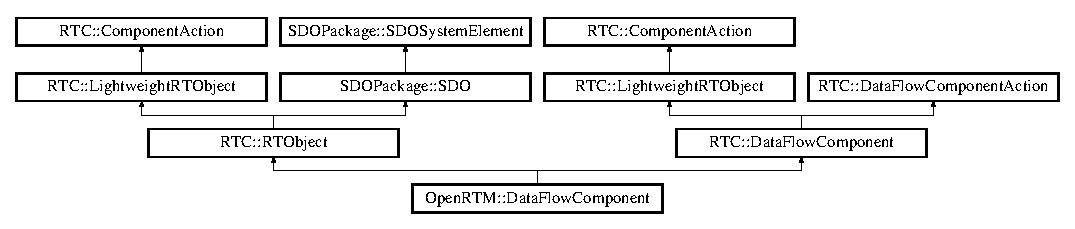
\includegraphics[height=2.62911cm]{interfaceOpenRTM_1_1DataFlowComponent}
\end{center}
\end{figure}
\subsection*{Public メソッド}
\begin{DoxyCompactItemize}
\item 
ComponentProfile {\bf get\_\-component\_\-profile} ()
\item 
PortServiceList {\bf get\_\-ports} ()
\item 
ReturnCode\_\-t {\bf initialize} ()
\item 
ReturnCode\_\-t {\bf finalize} ()
\item 
boolean {\bf is\_\-alive} (in ExecutionContext exec\_\-context)
\item 
ReturnCode\_\-t {\bf exit} ()
\item 
ExecutionContextHandle\_\-t {\bf attach\_\-context} (in ExecutionContext exec\_\-context)
\item 
ReturnCode\_\-t {\bf detach\_\-context} (in ExecutionContextHandle\_\-t exec\_\-handle)
\item 
ExecutionContext {\bf get\_\-context} (in ExecutionContextHandle\_\-t exec\_\-handle)
\item 
ExecutionContextList {\bf get\_\-owned\_\-contexts} ()
\begin{DoxyCompactList}\small\item\em get\_\-owned\_\-contexts \item\end{DoxyCompactList}\item 
ExecutionContextList {\bf get\_\-participating\_\-contexts} ()
\begin{DoxyCompactList}\small\item\em get\_\-participating\_\-contexts \item\end{DoxyCompactList}\item 
ExecutionContextHandle\_\-t {\bf get\_\-context\_\-handle} (in ExecutionContext cxt)
\item 
ReturnCode\_\-t {\bf on\_\-initialize} ()
\item 
ReturnCode\_\-t {\bf on\_\-finalize} ()
\item 
ReturnCode\_\-t {\bf on\_\-startup} (in ExecutionContextHandle\_\-t exec\_\-handle)
\item 
ReturnCode\_\-t {\bf on\_\-shutdown} (in ExecutionContextHandle\_\-t exec\_\-handle)
\item 
ReturnCode\_\-t {\bf on\_\-activated} (in ExecutionContextHandle\_\-t exec\_\-handle)
\item 
ReturnCode\_\-t {\bf on\_\-deactivated} (in ExecutionContextHandle\_\-t exec\_\-handle)
\item 
ReturnCode\_\-t {\bf on\_\-aborting} (in ExecutionContextHandle\_\-t exec\_\-handle)
\item 
ReturnCode\_\-t {\bf on\_\-error} (in ExecutionContextHandle\_\-t exec\_\-handle)
\item 
ReturnCode\_\-t {\bf on\_\-reset} (in ExecutionContextHandle\_\-t exec\_\-handle)
\item 
UniqueIdentifier {\bf get\_\-sdo\_\-id} ()  raises (NotAvailable, InternalError)
\item 
string {\bf get\_\-sdo\_\-type} ()  raises (NotAvailable, InternalError)
\item 
DeviceProfile {\bf get\_\-device\_\-profile} ()  raises (NotAvailable, InternalError)
\item 
ServiceProfileList {\bf get\_\-service\_\-profiles} ()  raises (NotAvailable, InternalError)
\item 
ServiceProfile {\bf get\_\-service\_\-profile} (in UniqueIdentifier id)  raises (InvalidParameter, NotAvailable, InternalError)
\item 
SDOService {\bf get\_\-sdo\_\-service} (in UniqueIdentifier id)  raises (InvalidParameter, NotAvailable, InternalError)
\item 
Configuration {\bf get\_\-configuration} ()  raises (InterfaceNotImplemented, NotAvailable, InternalError)
\item 
Monitoring {\bf get\_\-monitoring} ()  raises (InterfaceNotImplemented, NotAvailable, InternalError)
\item 
OrganizationList {\bf get\_\-organizations} ()  raises (NotAvailable, InternalError)
\item 
NVList {\bf get\_\-status\_\-list} ()  raises (NotAvailable, InternalError)
\item 
any {\bf get\_\-status} (in string nme)  raises (InvalidParameter, NotAvailable, InternalError)
\item 
OrganizationList {\bf get\_\-owned\_\-organizations} ()  raises (NotAvailable,InternalError)
\item 
ReturnCode\_\-t {\bf on\_\-execute} (in ExecutionContextHandle\_\-t exec\_\-handle)
\item 
ReturnCode\_\-t {\bf on\_\-state\_\-update} (in ExecutionContextHandle\_\-t exec\_\-handle)
\item 
ReturnCode\_\-t {\bf on\_\-rate\_\-changed} (in ExecutionContextHandle\_\-t exec\_\-handle)
\end{DoxyCompactItemize}


\subsection{関数}
\index{OpenRTM::DataFlowComponent@{OpenRTM::DataFlowComponent}!attach\_\-context@{attach\_\-context}}
\index{attach\_\-context@{attach\_\-context}!OpenRTM::DataFlowComponent@{OpenRTM::DataFlowComponent}}
\subsubsection[{attach\_\-context}]{\setlength{\rightskip}{0pt plus 5cm}ExecutionContextHandle\_\-t RTC::LightweightRTObject::attach\_\-context (in {\bf ExecutionContext} {\em exec\_\-context})\hspace{0.3cm}{\ttfamily  [inherited]}}\label{interfaceRTC_1_1LightweightRTObject_a48dbdbcac3254c29ad01d43a4ee5a00c}
\index{OpenRTM::DataFlowComponent@{OpenRTM::DataFlowComponent}!detach\_\-context@{detach\_\-context}}
\index{detach\_\-context@{detach\_\-context}!OpenRTM::DataFlowComponent@{OpenRTM::DataFlowComponent}}
\subsubsection[{detach\_\-context}]{\setlength{\rightskip}{0pt plus 5cm}ReturnCode\_\-t RTC::LightweightRTObject::detach\_\-context (in {\bf ExecutionContextHandle\_\-t} {\em exec\_\-handle})\hspace{0.3cm}{\ttfamily  [inherited]}}\label{interfaceRTC_1_1LightweightRTObject_a8eb94420ca08e8f7acaa778ed883b9a4}
\index{OpenRTM::DataFlowComponent@{OpenRTM::DataFlowComponent}!exit@{exit}}
\index{exit@{exit}!OpenRTM::DataFlowComponent@{OpenRTM::DataFlowComponent}}
\subsubsection[{exit}]{\setlength{\rightskip}{0pt plus 5cm}ReturnCode\_\-t RTC::LightweightRTObject::exit ()\hspace{0.3cm}{\ttfamily  [inherited]}}\label{interfaceRTC_1_1LightweightRTObject_a49bd940b6964fa80d696db15b45c2f87}
\index{OpenRTM::DataFlowComponent@{OpenRTM::DataFlowComponent}!finalize@{finalize}}
\index{finalize@{finalize}!OpenRTM::DataFlowComponent@{OpenRTM::DataFlowComponent}}
\subsubsection[{finalize}]{\setlength{\rightskip}{0pt plus 5cm}ReturnCode\_\-t RTC::LightweightRTObject::finalize ()\hspace{0.3cm}{\ttfamily  [inherited]}}\label{interfaceRTC_1_1LightweightRTObject_a23466f177b4289662ea035be831426ad}
\index{OpenRTM::DataFlowComponent@{OpenRTM::DataFlowComponent}!get\_\-component\_\-profile@{get\_\-component\_\-profile}}
\index{get\_\-component\_\-profile@{get\_\-component\_\-profile}!OpenRTM::DataFlowComponent@{OpenRTM::DataFlowComponent}}
\subsubsection[{get\_\-component\_\-profile}]{\setlength{\rightskip}{0pt plus 5cm}ComponentProfile RTC::RTObject::get\_\-component\_\-profile ()\hspace{0.3cm}{\ttfamily  [inherited]}}\label{interfaceRTC_1_1RTObject_aa75c245c8e7e0dd19148bbe5cefe4dcc}
\index{OpenRTM::DataFlowComponent@{OpenRTM::DataFlowComponent}!get\_\-configuration@{get\_\-configuration}}
\index{get\_\-configuration@{get\_\-configuration}!OpenRTM::DataFlowComponent@{OpenRTM::DataFlowComponent}}
\subsubsection[{get\_\-configuration}]{\setlength{\rightskip}{0pt plus 5cm}Configuration SDOPackage::SDO::get\_\-configuration ()  raises (InterfaceNotImplemented, NotAvailable, InternalError)\hspace{0.3cm}{\ttfamily  [inherited]}}\label{interfaceSDOPackage_1_1SDO_a89b6ff35b88f6212355e439a3a47c60a}
\index{OpenRTM::DataFlowComponent@{OpenRTM::DataFlowComponent}!get\_\-context@{get\_\-context}}
\index{get\_\-context@{get\_\-context}!OpenRTM::DataFlowComponent@{OpenRTM::DataFlowComponent}}
\subsubsection[{get\_\-context}]{\setlength{\rightskip}{0pt plus 5cm}ExecutionContext RTC::LightweightRTObject::get\_\-context (in {\bf ExecutionContextHandle\_\-t} {\em exec\_\-handle})\hspace{0.3cm}{\ttfamily  [inherited]}}\label{interfaceRTC_1_1LightweightRTObject_a7bb123faf81bcb57542c3a17f10948d6}
\index{OpenRTM::DataFlowComponent@{OpenRTM::DataFlowComponent}!get\_\-context\_\-handle@{get\_\-context\_\-handle}}
\index{get\_\-context\_\-handle@{get\_\-context\_\-handle}!OpenRTM::DataFlowComponent@{OpenRTM::DataFlowComponent}}
\subsubsection[{get\_\-context\_\-handle}]{\setlength{\rightskip}{0pt plus 5cm}ExecutionContextHandle\_\-t RTC::LightweightRTObject::get\_\-context\_\-handle (in {\bf ExecutionContext} {\em cxt})\hspace{0.3cm}{\ttfamily  [inherited]}}\label{interfaceRTC_1_1LightweightRTObject_af54041744c01d68026aa200276e12f45}
\#\#\# [����] \doxyref{RTC.idl}{p.}{RTC_8idl} �ˤϴޤޤ�Ƥ��ʤ���PIM�ˤϴޤޤ�Ƥ��롣 \#\#\# PIM���������� \index{OpenRTM::DataFlowComponent@{OpenRTM::DataFlowComponent}!get\_\-device\_\-profile@{get\_\-device\_\-profile}}
\index{get\_\-device\_\-profile@{get\_\-device\_\-profile}!OpenRTM::DataFlowComponent@{OpenRTM::DataFlowComponent}}
\subsubsection[{get\_\-device\_\-profile}]{\setlength{\rightskip}{0pt plus 5cm}DeviceProfile SDOPackage::SDO::get\_\-device\_\-profile ()  raises (NotAvailable, InternalError)\hspace{0.3cm}{\ttfamily  [inherited]}}\label{interfaceSDOPackage_1_1SDO_af96303b2025ea3e340303365b7ad9f0f}
\index{OpenRTM::DataFlowComponent@{OpenRTM::DataFlowComponent}!get\_\-monitoring@{get\_\-monitoring}}
\index{get\_\-monitoring@{get\_\-monitoring}!OpenRTM::DataFlowComponent@{OpenRTM::DataFlowComponent}}
\subsubsection[{get\_\-monitoring}]{\setlength{\rightskip}{0pt plus 5cm}Monitoring SDOPackage::SDO::get\_\-monitoring ()  raises (InterfaceNotImplemented, NotAvailable, InternalError)\hspace{0.3cm}{\ttfamily  [inherited]}}\label{interfaceSDOPackage_1_1SDO_a7db6dded91e964ec26085d1fa8f540c9}
\index{OpenRTM::DataFlowComponent@{OpenRTM::DataFlowComponent}!get\_\-organizations@{get\_\-organizations}}
\index{get\_\-organizations@{get\_\-organizations}!OpenRTM::DataFlowComponent@{OpenRTM::DataFlowComponent}}
\subsubsection[{get\_\-organizations}]{\setlength{\rightskip}{0pt plus 5cm}OrganizationList SDOPackage::SDO::get\_\-organizations ()  raises (NotAvailable, InternalError)\hspace{0.3cm}{\ttfamily  [inherited]}}\label{interfaceSDOPackage_1_1SDO_aadb5f8bb6eb2529189d3779940607edd}
\index{OpenRTM::DataFlowComponent@{OpenRTM::DataFlowComponent}!get\_\-owned\_\-contexts@{get\_\-owned\_\-contexts}}
\index{get\_\-owned\_\-contexts@{get\_\-owned\_\-contexts}!OpenRTM::DataFlowComponent@{OpenRTM::DataFlowComponent}}
\subsubsection[{get\_\-owned\_\-contexts}]{\setlength{\rightskip}{0pt plus 5cm}ExecutionContextList RTC::LightweightRTObject::get\_\-owned\_\-contexts ()\hspace{0.3cm}{\ttfamily  [inherited]}}\label{interfaceRTC_1_1LightweightRTObject_aea9dd2a447cc3ddc55f20aab698da408}


get\_\-owned\_\-contexts 

\subsection{Description}\label{interfaceRTC_1_1LightweightRTObject_Description}
���� \doxyref{RTC}{p.}{namespaceRTC} ����ͭ���� \doxyref{ExecutionContext}{p.}{interfaceRTC_1_1ExecutionContext} �Υꥹ�Ȥ�������롣 \index{OpenRTM::DataFlowComponent@{OpenRTM::DataFlowComponent}!get\_\-owned\_\-organizations@{get\_\-owned\_\-organizations}}
\index{get\_\-owned\_\-organizations@{get\_\-owned\_\-organizations}!OpenRTM::DataFlowComponent@{OpenRTM::DataFlowComponent}}
\subsubsection[{get\_\-owned\_\-organizations}]{\setlength{\rightskip}{0pt plus 5cm}OrganizationList SDOPackage::SDOSystemElement::get\_\-owned\_\-organizations ()  raises (NotAvailable,InternalError)\hspace{0.3cm}{\ttfamily  [inherited]}}\label{interfaceSDOPackage_1_1SDOSystemElement_a81238047c5dfa47d2cf3ebce1b78b240}
\index{OpenRTM::DataFlowComponent@{OpenRTM::DataFlowComponent}!get\_\-participating\_\-contexts@{get\_\-participating\_\-contexts}}
\index{get\_\-participating\_\-contexts@{get\_\-participating\_\-contexts}!OpenRTM::DataFlowComponent@{OpenRTM::DataFlowComponent}}
\subsubsection[{get\_\-participating\_\-contexts}]{\setlength{\rightskip}{0pt plus 5cm}ExecutionContextList RTC::LightweightRTObject::get\_\-participating\_\-contexts ()\hspace{0.3cm}{\ttfamily  [inherited]}}\label{interfaceRTC_1_1LightweightRTObject_af2224880b89275ecf82efad0999b022a}


get\_\-participating\_\-contexts 

\subsection{Description}\label{interfaceRTC_1_1LightweightRTObject_Description}
���� \doxyref{RTC}{p.}{namespaceRTC} �����ä��Ƥ��뤹�٤Ƥ� \doxyref{ExecutionContext}{p.}{interfaceRTC_1_1ExecutionContext} �Υꥹ�Ȥ�������롣\subsection{Semantics}\label{interfaceRTC_1_1LightweightRTObject_Semantics}
���Υꥹ�Ȥ˴ޤޤ��¹ԥ���ƥ����Ȥϡ�attach\_\-context ���Ƥӽ� ����뤴�Ȥˡ��ꥹ�Ȥ��ɲä��졢detach\_\-context ���ƤӽФ���뤴 �Ȥˡ��ꥹ�Ȥ���������롣 \index{OpenRTM::DataFlowComponent@{OpenRTM::DataFlowComponent}!get\_\-ports@{get\_\-ports}}
\index{get\_\-ports@{get\_\-ports}!OpenRTM::DataFlowComponent@{OpenRTM::DataFlowComponent}}
\subsubsection[{get\_\-ports}]{\setlength{\rightskip}{0pt plus 5cm}PortServiceList RTC::RTObject::get\_\-ports ()\hspace{0.3cm}{\ttfamily  [inherited]}}\label{interfaceRTC_1_1RTObject_a4e21edb9c244ed8469cb1fb2de48e158}
\index{OpenRTM::DataFlowComponent@{OpenRTM::DataFlowComponent}!get\_\-sdo\_\-id@{get\_\-sdo\_\-id}}
\index{get\_\-sdo\_\-id@{get\_\-sdo\_\-id}!OpenRTM::DataFlowComponent@{OpenRTM::DataFlowComponent}}
\subsubsection[{get\_\-sdo\_\-id}]{\setlength{\rightskip}{0pt plus 5cm}UniqueIdentifier SDOPackage::SDO::get\_\-sdo\_\-id ()  raises (NotAvailable, InternalError)\hspace{0.3cm}{\ttfamily  [inherited]}}\label{interfaceSDOPackage_1_1SDO_a08ccbbb1855dff27c598c38ce0c5aab1}
\index{OpenRTM::DataFlowComponent@{OpenRTM::DataFlowComponent}!get\_\-sdo\_\-service@{get\_\-sdo\_\-service}}
\index{get\_\-sdo\_\-service@{get\_\-sdo\_\-service}!OpenRTM::DataFlowComponent@{OpenRTM::DataFlowComponent}}
\subsubsection[{get\_\-sdo\_\-service}]{\setlength{\rightskip}{0pt plus 5cm}SDOService SDOPackage::SDO::get\_\-sdo\_\-service (in {\bf UniqueIdentifier} {\em id})  raises (InvalidParameter, NotAvailable, InternalError)\hspace{0.3cm}{\ttfamily  [inherited]}}\label{interfaceSDOPackage_1_1SDO_a7d612d97207fecaf134959b93c6b3e60}
\index{OpenRTM::DataFlowComponent@{OpenRTM::DataFlowComponent}!get\_\-sdo\_\-type@{get\_\-sdo\_\-type}}
\index{get\_\-sdo\_\-type@{get\_\-sdo\_\-type}!OpenRTM::DataFlowComponent@{OpenRTM::DataFlowComponent}}
\subsubsection[{get\_\-sdo\_\-type}]{\setlength{\rightskip}{0pt plus 5cm}string SDOPackage::SDO::get\_\-sdo\_\-type ()  raises (NotAvailable, InternalError)\hspace{0.3cm}{\ttfamily  [inherited]}}\label{interfaceSDOPackage_1_1SDO_a2b4141376be89eb90fd4904643476320}
\index{OpenRTM::DataFlowComponent@{OpenRTM::DataFlowComponent}!get\_\-service\_\-profile@{get\_\-service\_\-profile}}
\index{get\_\-service\_\-profile@{get\_\-service\_\-profile}!OpenRTM::DataFlowComponent@{OpenRTM::DataFlowComponent}}
\subsubsection[{get\_\-service\_\-profile}]{\setlength{\rightskip}{0pt plus 5cm}ServiceProfile SDOPackage::SDO::get\_\-service\_\-profile (in {\bf UniqueIdentifier} {\em id})  raises (InvalidParameter, NotAvailable, InternalError)\hspace{0.3cm}{\ttfamily  [inherited]}}\label{interfaceSDOPackage_1_1SDO_a5ea1929e10ccc5e8b5896c4b0fbee635}
\index{OpenRTM::DataFlowComponent@{OpenRTM::DataFlowComponent}!get\_\-service\_\-profiles@{get\_\-service\_\-profiles}}
\index{get\_\-service\_\-profiles@{get\_\-service\_\-profiles}!OpenRTM::DataFlowComponent@{OpenRTM::DataFlowComponent}}
\subsubsection[{get\_\-service\_\-profiles}]{\setlength{\rightskip}{0pt plus 5cm}ServiceProfileList SDOPackage::SDO::get\_\-service\_\-profiles ()  raises (NotAvailable, InternalError)\hspace{0.3cm}{\ttfamily  [inherited]}}\label{interfaceSDOPackage_1_1SDO_af455c384fa54ab6872d28db1baec3a1d}
\index{OpenRTM::DataFlowComponent@{OpenRTM::DataFlowComponent}!get\_\-status@{get\_\-status}}
\index{get\_\-status@{get\_\-status}!OpenRTM::DataFlowComponent@{OpenRTM::DataFlowComponent}}
\subsubsection[{get\_\-status}]{\setlength{\rightskip}{0pt plus 5cm}any SDOPackage::SDO::get\_\-status (in string {\em nme})  raises (InvalidParameter, NotAvailable, InternalError)\hspace{0.3cm}{\ttfamily  [inherited]}}\label{interfaceSDOPackage_1_1SDO_a2655f624a38b590593154c8a8c11e6e8}
\index{OpenRTM::DataFlowComponent@{OpenRTM::DataFlowComponent}!get\_\-status\_\-list@{get\_\-status\_\-list}}
\index{get\_\-status\_\-list@{get\_\-status\_\-list}!OpenRTM::DataFlowComponent@{OpenRTM::DataFlowComponent}}
\subsubsection[{get\_\-status\_\-list}]{\setlength{\rightskip}{0pt plus 5cm}NVList SDOPackage::SDO::get\_\-status\_\-list ()  raises (NotAvailable, InternalError)\hspace{0.3cm}{\ttfamily  [inherited]}}\label{interfaceSDOPackage_1_1SDO_ae019ba73a5675a871701153bc56db14c}
\index{OpenRTM::DataFlowComponent@{OpenRTM::DataFlowComponent}!initialize@{initialize}}
\index{initialize@{initialize}!OpenRTM::DataFlowComponent@{OpenRTM::DataFlowComponent}}
\subsubsection[{initialize}]{\setlength{\rightskip}{0pt plus 5cm}ReturnCode\_\-t RTC::LightweightRTObject::initialize ()\hspace{0.3cm}{\ttfamily  [inherited]}}\label{interfaceRTC_1_1LightweightRTObject_afb28c4d97677804da09488578b840eb5}
\index{OpenRTM::DataFlowComponent@{OpenRTM::DataFlowComponent}!is\_\-alive@{is\_\-alive}}
\index{is\_\-alive@{is\_\-alive}!OpenRTM::DataFlowComponent@{OpenRTM::DataFlowComponent}}
\subsubsection[{is\_\-alive}]{\setlength{\rightskip}{0pt plus 5cm}boolean RTC::LightweightRTObject::is\_\-alive (in {\bf ExecutionContext} {\em exec\_\-context})\hspace{0.3cm}{\ttfamily  [inherited]}}\label{interfaceRTC_1_1LightweightRTObject_aa07c8c299b0addc49887508c1ee7be27}
\index{OpenRTM::DataFlowComponent@{OpenRTM::DataFlowComponent}!on\_\-aborting@{on\_\-aborting}}
\index{on\_\-aborting@{on\_\-aborting}!OpenRTM::DataFlowComponent@{OpenRTM::DataFlowComponent}}
\subsubsection[{on\_\-aborting}]{\setlength{\rightskip}{0pt plus 5cm}ReturnCode\_\-t RTC::ComponentAction::on\_\-aborting (in {\bf ExecutionContextHandle\_\-t} {\em exec\_\-handle})\hspace{0.3cm}{\ttfamily  [inherited]}}\label{interfaceRTC_1_1ComponentAction_a876e58ebcea16c307e131b3e6a58ddbe}
\index{OpenRTM::DataFlowComponent@{OpenRTM::DataFlowComponent}!on\_\-activated@{on\_\-activated}}
\index{on\_\-activated@{on\_\-activated}!OpenRTM::DataFlowComponent@{OpenRTM::DataFlowComponent}}
\subsubsection[{on\_\-activated}]{\setlength{\rightskip}{0pt plus 5cm}ReturnCode\_\-t RTC::ComponentAction::on\_\-activated (in {\bf ExecutionContextHandle\_\-t} {\em exec\_\-handle})\hspace{0.3cm}{\ttfamily  [inherited]}}\label{interfaceRTC_1_1ComponentAction_a4f51f627067d0c54e89c4c0827fa6432}
\index{OpenRTM::DataFlowComponent@{OpenRTM::DataFlowComponent}!on\_\-deactivated@{on\_\-deactivated}}
\index{on\_\-deactivated@{on\_\-deactivated}!OpenRTM::DataFlowComponent@{OpenRTM::DataFlowComponent}}
\subsubsection[{on\_\-deactivated}]{\setlength{\rightskip}{0pt plus 5cm}ReturnCode\_\-t RTC::ComponentAction::on\_\-deactivated (in {\bf ExecutionContextHandle\_\-t} {\em exec\_\-handle})\hspace{0.3cm}{\ttfamily  [inherited]}}\label{interfaceRTC_1_1ComponentAction_aa5f9cfb9677ba685be333ad666c87f88}
\index{OpenRTM::DataFlowComponent@{OpenRTM::DataFlowComponent}!on\_\-error@{on\_\-error}}
\index{on\_\-error@{on\_\-error}!OpenRTM::DataFlowComponent@{OpenRTM::DataFlowComponent}}
\subsubsection[{on\_\-error}]{\setlength{\rightskip}{0pt plus 5cm}ReturnCode\_\-t RTC::ComponentAction::on\_\-error (in {\bf ExecutionContextHandle\_\-t} {\em exec\_\-handle})\hspace{0.3cm}{\ttfamily  [inherited]}}\label{interfaceRTC_1_1ComponentAction_a110fdde803e9b13f27308b897439962a}
\index{OpenRTM::DataFlowComponent@{OpenRTM::DataFlowComponent}!on\_\-execute@{on\_\-execute}}
\index{on\_\-execute@{on\_\-execute}!OpenRTM::DataFlowComponent@{OpenRTM::DataFlowComponent}}
\subsubsection[{on\_\-execute}]{\setlength{\rightskip}{0pt plus 5cm}ReturnCode\_\-t RTC::DataFlowComponentAction::on\_\-execute (in {\bf ExecutionContextHandle\_\-t} {\em exec\_\-handle})\hspace{0.3cm}{\ttfamily  [inherited]}}\label{interfaceRTC_1_1DataFlowComponentAction_a70a1d7f32e03c719dd8949ea5d0be214}
\index{OpenRTM::DataFlowComponent@{OpenRTM::DataFlowComponent}!on\_\-finalize@{on\_\-finalize}}
\index{on\_\-finalize@{on\_\-finalize}!OpenRTM::DataFlowComponent@{OpenRTM::DataFlowComponent}}
\subsubsection[{on\_\-finalize}]{\setlength{\rightskip}{0pt plus 5cm}ReturnCode\_\-t RTC::ComponentAction::on\_\-finalize ()\hspace{0.3cm}{\ttfamily  [inherited]}}\label{interfaceRTC_1_1ComponentAction_a9c9e2d638cd2b748609be8a23410aedc}
\index{OpenRTM::DataFlowComponent@{OpenRTM::DataFlowComponent}!on\_\-initialize@{on\_\-initialize}}
\index{on\_\-initialize@{on\_\-initialize}!OpenRTM::DataFlowComponent@{OpenRTM::DataFlowComponent}}
\subsubsection[{on\_\-initialize}]{\setlength{\rightskip}{0pt plus 5cm}ReturnCode\_\-t RTC::ComponentAction::on\_\-initialize ()\hspace{0.3cm}{\ttfamily  [inherited]}}\label{interfaceRTC_1_1ComponentAction_a8703b183bc1bed9e2fd3ecac126cb231}
\index{OpenRTM::DataFlowComponent@{OpenRTM::DataFlowComponent}!on\_\-rate\_\-changed@{on\_\-rate\_\-changed}}
\index{on\_\-rate\_\-changed@{on\_\-rate\_\-changed}!OpenRTM::DataFlowComponent@{OpenRTM::DataFlowComponent}}
\subsubsection[{on\_\-rate\_\-changed}]{\setlength{\rightskip}{0pt plus 5cm}ReturnCode\_\-t RTC::DataFlowComponentAction::on\_\-rate\_\-changed (in {\bf ExecutionContextHandle\_\-t} {\em exec\_\-handle})\hspace{0.3cm}{\ttfamily  [inherited]}}\label{interfaceRTC_1_1DataFlowComponentAction_a6d010e52880cb1e4228817041a6ac518}
\index{OpenRTM::DataFlowComponent@{OpenRTM::DataFlowComponent}!on\_\-reset@{on\_\-reset}}
\index{on\_\-reset@{on\_\-reset}!OpenRTM::DataFlowComponent@{OpenRTM::DataFlowComponent}}
\subsubsection[{on\_\-reset}]{\setlength{\rightskip}{0pt plus 5cm}ReturnCode\_\-t RTC::ComponentAction::on\_\-reset (in {\bf ExecutionContextHandle\_\-t} {\em exec\_\-handle})\hspace{0.3cm}{\ttfamily  [inherited]}}\label{interfaceRTC_1_1ComponentAction_adb0e61bff251337d79c7c7d050d8304e}
\index{OpenRTM::DataFlowComponent@{OpenRTM::DataFlowComponent}!on\_\-shutdown@{on\_\-shutdown}}
\index{on\_\-shutdown@{on\_\-shutdown}!OpenRTM::DataFlowComponent@{OpenRTM::DataFlowComponent}}
\subsubsection[{on\_\-shutdown}]{\setlength{\rightskip}{0pt plus 5cm}ReturnCode\_\-t RTC::ComponentAction::on\_\-shutdown (in {\bf ExecutionContextHandle\_\-t} {\em exec\_\-handle})\hspace{0.3cm}{\ttfamily  [inherited]}}\label{interfaceRTC_1_1ComponentAction_accc47711344c811c9bdba0d66a3048f2}
\index{OpenRTM::DataFlowComponent@{OpenRTM::DataFlowComponent}!on\_\-startup@{on\_\-startup}}
\index{on\_\-startup@{on\_\-startup}!OpenRTM::DataFlowComponent@{OpenRTM::DataFlowComponent}}
\subsubsection[{on\_\-startup}]{\setlength{\rightskip}{0pt plus 5cm}ReturnCode\_\-t RTC::ComponentAction::on\_\-startup (in {\bf ExecutionContextHandle\_\-t} {\em exec\_\-handle})\hspace{0.3cm}{\ttfamily  [inherited]}}\label{interfaceRTC_1_1ComponentAction_ac305f00c92f4650cf4fc798aac37eef2}
\index{OpenRTM::DataFlowComponent@{OpenRTM::DataFlowComponent}!on\_\-state\_\-update@{on\_\-state\_\-update}}
\index{on\_\-state\_\-update@{on\_\-state\_\-update}!OpenRTM::DataFlowComponent@{OpenRTM::DataFlowComponent}}
\subsubsection[{on\_\-state\_\-update}]{\setlength{\rightskip}{0pt plus 5cm}ReturnCode\_\-t RTC::DataFlowComponentAction::on\_\-state\_\-update (in {\bf ExecutionContextHandle\_\-t} {\em exec\_\-handle})\hspace{0.3cm}{\ttfamily  [inherited]}}\label{interfaceRTC_1_1DataFlowComponentAction_a10aed288388578b108c9766f67997668}


このインタフェースの説明は次のファイルから生成されました:\begin{DoxyCompactItemize}
\item 
{\bf OpenRTM.idl}\end{DoxyCompactItemize}

\section{RTC::DataFlowComponentAction Interface Reference}
\label{interfaceRTC_1_1DataFlowComponentAction}\index{RTC::DataFlowComponentAction@{RTC::DataFlowComponentAction}}


\doxyref{DataFlowComponentAction}{p.}{interfaceRTC_1_1DataFlowComponentAction}.  




{\ttfamily import \char`\"{}RTC.idl\char`\"{};}

Inheritance diagram for RTC::DataFlowComponentAction:\begin{figure}[H]
\begin{center}
\leavevmode
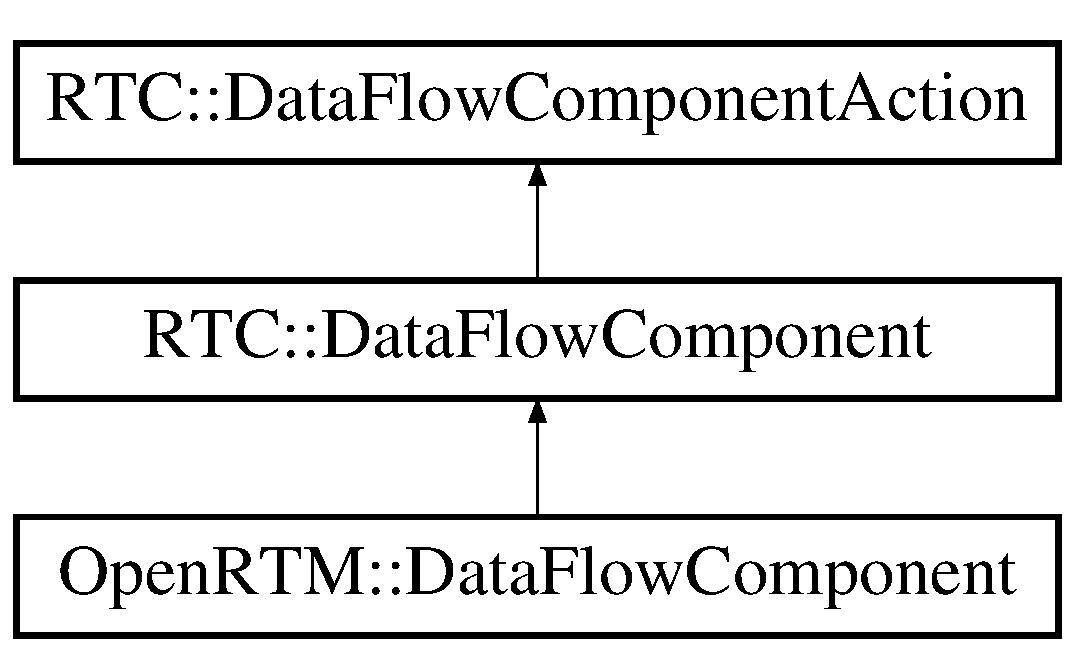
\includegraphics[height=3cm]{interfaceRTC_1_1DataFlowComponentAction}
\end{center}
\end{figure}
\subsection*{Public Member Functions}
\begin{DoxyCompactItemize}
\item 
{\bf ReturnCode\_\-t} {\bf on\_\-execute} (in {\bf ExecutionContextHandle\_\-t} exec\_\-handle)
\begin{DoxyCompactList}\small\item\em on\_\-execute \item\end{DoxyCompactList}\item 
{\bf ReturnCode\_\-t} {\bf on\_\-state\_\-update} (in {\bf ExecutionContextHandle\_\-t} exec\_\-handle)
\begin{DoxyCompactList}\small\item\em on\_\-state\_\-update \item\end{DoxyCompactList}\item 
{\bf ReturnCode\_\-t} {\bf on\_\-rate\_\-changed} (in {\bf ExecutionContextHandle\_\-t} exec\_\-handle)
\begin{DoxyCompactList}\small\item\em on\_\-rate\_\-changed \item\end{DoxyCompactList}\end{DoxyCompactItemize}


\subsection{Detailed Description}
\doxyref{DataFlowComponentAction}{p.}{interfaceRTC_1_1DataFlowComponentAction}. \subsection{Description}\label{namespaceRTC_Description}
\doxyref{DataFlowComponentAction}{p.}{interfaceRTC_1_1DataFlowComponentAction} is a companion to \doxyref{ComponentAction}{p.}{interfaceRTC_1_1ComponentAction} (see Section 5.2.2.4) that provides additional callbacks for intercepting the two execution passes defined in Section 5.3.1.1.2. 

\subsection{Member Function Documentation}
\index{RTC::DataFlowComponentAction@{RTC::DataFlowComponentAction}!on\_\-execute@{on\_\-execute}}
\index{on\_\-execute@{on\_\-execute}!RTC::DataFlowComponentAction@{RTC::DataFlowComponentAction}}
\subsubsection[{on\_\-execute}]{\setlength{\rightskip}{0pt plus 5cm}{\bf ReturnCode\_\-t} RTC::DataFlowComponentAction::on\_\-execute (in {\bf ExecutionContextHandle\_\-t} {\em exec\_\-handle})}\label{interfaceRTC_1_1DataFlowComponentAction_a70a1d7f32e03c719dd8949ea5d0be214}


on\_\-execute 

\subsection{Description}\label{namespaceRTC_Description}
This operation will be invoked periodically at the rate of the given execution context as long as the following conditions hold:


\begin{DoxyItemize}
\item The \doxyref{RTC}{p.}{namespaceRTC} is Active.
\end{DoxyItemize}


\begin{DoxyItemize}
\item The given execution context is Running.
\end{DoxyItemize}\subsection{Semantics}\label{namespaceRTC_Semantics}
This callback occurs during the first execution pass.\subsection{Constraints}\label{interfaceRTC_1_1LightweightRTObject_Constraints}

\begin{DoxyItemize}
\item The execution context of the given context shall be PERIODIC. 
\end{DoxyItemize}\index{RTC::DataFlowComponentAction@{RTC::DataFlowComponentAction}!on\_\-rate\_\-changed@{on\_\-rate\_\-changed}}
\index{on\_\-rate\_\-changed@{on\_\-rate\_\-changed}!RTC::DataFlowComponentAction@{RTC::DataFlowComponentAction}}
\subsubsection[{on\_\-rate\_\-changed}]{\setlength{\rightskip}{0pt plus 5cm}{\bf ReturnCode\_\-t} RTC::DataFlowComponentAction::on\_\-rate\_\-changed (in {\bf ExecutionContextHandle\_\-t} {\em exec\_\-handle})}\label{interfaceRTC_1_1DataFlowComponentAction_a6d010e52880cb1e4228817041a6ac518}


on\_\-rate\_\-changed 

\subsection{Description}\label{namespaceRTC_Description}
This operation is a notification that the rate of the indicated execution context (see Section 5.2.2.6.4) has changed.\subsection{Constraints}\label{interfaceRTC_1_1LightweightRTObject_Constraints}

\begin{DoxyItemize}
\item The execution context of the given context shall be PERIODIC. 
\end{DoxyItemize}\index{RTC::DataFlowComponentAction@{RTC::DataFlowComponentAction}!on\_\-state\_\-update@{on\_\-state\_\-update}}
\index{on\_\-state\_\-update@{on\_\-state\_\-update}!RTC::DataFlowComponentAction@{RTC::DataFlowComponentAction}}
\subsubsection[{on\_\-state\_\-update}]{\setlength{\rightskip}{0pt plus 5cm}{\bf ReturnCode\_\-t} RTC::DataFlowComponentAction::on\_\-state\_\-update (in {\bf ExecutionContextHandle\_\-t} {\em exec\_\-handle})}\label{interfaceRTC_1_1DataFlowComponentAction_a10aed288388578b108c9766f67997668}


on\_\-state\_\-update 

\subsection{Description}\label{namespaceRTC_Description}
This operation will be invoked periodically at the rate of the given execution context as long as the following conditions hold:


\begin{DoxyItemize}
\item The \doxyref{RTC}{p.}{namespaceRTC} is Active.
\end{DoxyItemize}


\begin{DoxyItemize}
\item The given execution context is Running.
\end{DoxyItemize}\subsection{Semantics}\label{namespaceRTC_Semantics}
This callback occurs during the second execution pass.\subsection{Constraints}\label{interfaceRTC_1_1LightweightRTObject_Constraints}

\begin{DoxyItemize}
\item The execution context of the given context shall be PERIODIC. 
\end{DoxyItemize}

The documentation for this interface was generated from the following file:\begin{DoxyCompactItemize}
\item 
{\bf RTC.idl}\end{DoxyCompactItemize}

\section{構造体 SDOPackage::DeviceProfile}
\label{structSDOPackage_1_1DeviceProfile}\index{SDOPackage::DeviceProfile@{SDOPackage::DeviceProfile}}


{\ttfamily import \char`\"{}SDOPackage.idl\char`\"{};}

\subsection*{Public 変数}
\begin{DoxyCompactItemize}
\item 
string {\bf device\_\-type}
\item 
string {\bf manufacturer}
\item 
string {\bf model}
\item 
string {\bf version}
\item 
{\bf NVList} {\bf properties}
\end{DoxyCompactItemize}


\subsection{変数}
\index{SDOPackage::DeviceProfile@{SDOPackage::DeviceProfile}!device\_\-type@{device\_\-type}}
\index{device\_\-type@{device\_\-type}!SDOPackage::DeviceProfile@{SDOPackage::DeviceProfile}}
\subsubsection[{device\_\-type}]{\setlength{\rightskip}{0pt plus 5cm}string {\bf SDOPackage::DeviceProfile::device\_\-type}}\label{structSDOPackage_1_1DeviceProfile_a41856ed05da8e78d4e853c44fb82a0f0}
\index{SDOPackage::DeviceProfile@{SDOPackage::DeviceProfile}!manufacturer@{manufacturer}}
\index{manufacturer@{manufacturer}!SDOPackage::DeviceProfile@{SDOPackage::DeviceProfile}}
\subsubsection[{manufacturer}]{\setlength{\rightskip}{0pt plus 5cm}string {\bf SDOPackage::DeviceProfile::manufacturer}}\label{structSDOPackage_1_1DeviceProfile_a7f04867de10ac0a3f2dba9d1e672e94c}
\index{SDOPackage::DeviceProfile@{SDOPackage::DeviceProfile}!model@{model}}
\index{model@{model}!SDOPackage::DeviceProfile@{SDOPackage::DeviceProfile}}
\subsubsection[{model}]{\setlength{\rightskip}{0pt plus 5cm}string {\bf SDOPackage::DeviceProfile::model}}\label{structSDOPackage_1_1DeviceProfile_a36b90434d0fc86721269a418667af436}
\index{SDOPackage::DeviceProfile@{SDOPackage::DeviceProfile}!properties@{properties}}
\index{properties@{properties}!SDOPackage::DeviceProfile@{SDOPackage::DeviceProfile}}
\subsubsection[{properties}]{\setlength{\rightskip}{0pt plus 5cm}{\bf NVList} {\bf SDOPackage::DeviceProfile::properties}}\label{structSDOPackage_1_1DeviceProfile_a6945952e1a03ed66975f8880ad66cc8b}
\index{SDOPackage::DeviceProfile@{SDOPackage::DeviceProfile}!version@{version}}
\index{version@{version}!SDOPackage::DeviceProfile@{SDOPackage::DeviceProfile}}
\subsubsection[{version}]{\setlength{\rightskip}{0pt plus 5cm}string {\bf SDOPackage::DeviceProfile::version}}\label{structSDOPackage_1_1DeviceProfile_adcf7a5ff087fb27effb546f9adcd9c1e}


この構造体の説明は次のファイルから生成されました:\begin{DoxyCompactItemize}
\item 
{\bf SDOPackage.idl}\end{DoxyCompactItemize}

\section{構造体 SDOPackage::EnumerationType}
\label{structSDOPackage_1_1EnumerationType}\index{SDOPackage::EnumerationType@{SDOPackage::EnumerationType}}


{\ttfamily import \char`\"{}SDOPackage.idl\char`\"{};}

\subsection*{Public 変数}
\begin{DoxyCompactItemize}
\item 
{\bf StringList} {\bf enumerated\_\-values}
\end{DoxyCompactItemize}


\subsection{変数}
\index{SDOPackage::EnumerationType@{SDOPackage::EnumerationType}!enumerated\_\-values@{enumerated\_\-values}}
\index{enumerated\_\-values@{enumerated\_\-values}!SDOPackage::EnumerationType@{SDOPackage::EnumerationType}}
\subsubsection[{enumerated\_\-values}]{\setlength{\rightskip}{0pt plus 5cm}{\bf StringList} {\bf SDOPackage::EnumerationType::enumerated\_\-values}}\label{structSDOPackage_1_1EnumerationType_a9b6c16891322e19809a402b850cb9243}


この構造体の説明は次のファイルから生成されました:\begin{DoxyCompactItemize}
\item 
{\bf SDOPackage.idl}\end{DoxyCompactItemize}

\section{インタフェース RTC::ExecutionContext}
\label{interfaceRTC_1_1ExecutionContext}\index{RTC::ExecutionContext@{RTC::ExecutionContext}}


{\ttfamily import \char`\"{}RTC.idl\char`\"{};}

RTC::ExecutionContextに対する継承グラフ\begin{figure}[H]
\begin{center}
\leavevmode
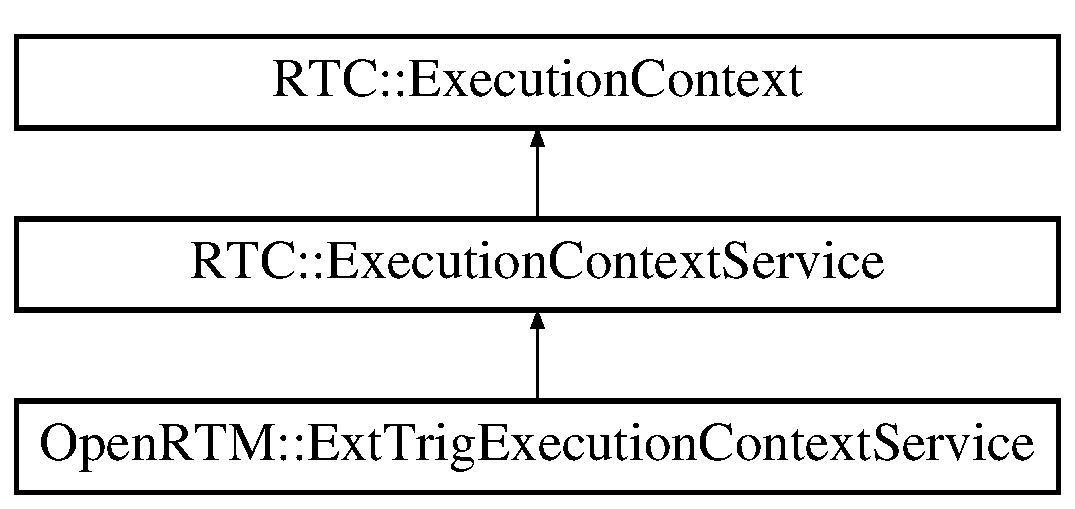
\includegraphics[height=3cm]{interfaceRTC_1_1ExecutionContext}
\end{center}
\end{figure}
\subsection*{Public メソッド}
\begin{DoxyCompactItemize}
\item 
boolean {\bf is\_\-running} ()
\item 
{\bf ReturnCode\_\-t} {\bf start} ()
\item 
{\bf ReturnCode\_\-t} {\bf stop} ()
\item 
double {\bf get\_\-rate} ()
\item 
{\bf ReturnCode\_\-t} {\bf set\_\-rate} (in double rate)
\item 
{\bf ReturnCode\_\-t} {\bf add\_\-component} (in {\bf LightweightRTObject} comp)
\item 
{\bf ReturnCode\_\-t} {\bf remove\_\-component} (in {\bf LightweightRTObject} comp)
\item 
{\bf ReturnCode\_\-t} {\bf activate\_\-component} (in {\bf LightweightRTObject} comp)
\item 
{\bf ReturnCode\_\-t} {\bf deactivate\_\-component} (in {\bf LightweightRTObject} comp)
\item 
{\bf ReturnCode\_\-t} {\bf reset\_\-component} (in {\bf LightweightRTObject} comp)
\item 
{\bf LifeCycleState} {\bf get\_\-component\_\-state} (in {\bf LightweightRTObject} comp)
\item 
{\bf ExecutionKind} {\bf get\_\-kind} ()
\end{DoxyCompactItemize}


\subsection{関数}
\index{RTC::ExecutionContext@{RTC::ExecutionContext}!activate\_\-component@{activate\_\-component}}
\index{activate\_\-component@{activate\_\-component}!RTC::ExecutionContext@{RTC::ExecutionContext}}
\subsubsection[{activate\_\-component}]{\setlength{\rightskip}{0pt plus 5cm}{\bf ReturnCode\_\-t} RTC::ExecutionContext::activate\_\-component (in {\bf LightweightRTObject} {\em comp})}\label{interfaceRTC_1_1ExecutionContext_af4a8aeab4a5e71e731b89556ef3e33e1}
\index{RTC::ExecutionContext@{RTC::ExecutionContext}!add\_\-component@{add\_\-component}}
\index{add\_\-component@{add\_\-component}!RTC::ExecutionContext@{RTC::ExecutionContext}}
\subsubsection[{add\_\-component}]{\setlength{\rightskip}{0pt plus 5cm}{\bf ReturnCode\_\-t} RTC::ExecutionContext::add\_\-component (in {\bf LightweightRTObject} {\em comp})}\label{interfaceRTC_1_1ExecutionContext_a7ac1a5b9820e571153db730c9369b600}
\index{RTC::ExecutionContext@{RTC::ExecutionContext}!deactivate\_\-component@{deactivate\_\-component}}
\index{deactivate\_\-component@{deactivate\_\-component}!RTC::ExecutionContext@{RTC::ExecutionContext}}
\subsubsection[{deactivate\_\-component}]{\setlength{\rightskip}{0pt plus 5cm}{\bf ReturnCode\_\-t} RTC::ExecutionContext::deactivate\_\-component (in {\bf LightweightRTObject} {\em comp})}\label{interfaceRTC_1_1ExecutionContext_a82a23124035a957f2191b520a011e870}
\index{RTC::ExecutionContext@{RTC::ExecutionContext}!get\_\-component\_\-state@{get\_\-component\_\-state}}
\index{get\_\-component\_\-state@{get\_\-component\_\-state}!RTC::ExecutionContext@{RTC::ExecutionContext}}
\subsubsection[{get\_\-component\_\-state}]{\setlength{\rightskip}{0pt plus 5cm}{\bf LifeCycleState} RTC::ExecutionContext::get\_\-component\_\-state (in {\bf LightweightRTObject} {\em comp})}\label{interfaceRTC_1_1ExecutionContext_a51a0396327ec0bab96f06a246032fc84}
\index{RTC::ExecutionContext@{RTC::ExecutionContext}!get\_\-kind@{get\_\-kind}}
\index{get\_\-kind@{get\_\-kind}!RTC::ExecutionContext@{RTC::ExecutionContext}}
\subsubsection[{get\_\-kind}]{\setlength{\rightskip}{0pt plus 5cm}{\bf ExecutionKind} RTC::ExecutionContext::get\_\-kind ()}\label{interfaceRTC_1_1ExecutionContext_aa7175c37b85b78b90ea5468a4f1379b0}
\index{RTC::ExecutionContext@{RTC::ExecutionContext}!get\_\-rate@{get\_\-rate}}
\index{get\_\-rate@{get\_\-rate}!RTC::ExecutionContext@{RTC::ExecutionContext}}
\subsubsection[{get\_\-rate}]{\setlength{\rightskip}{0pt plus 5cm}double RTC::ExecutionContext::get\_\-rate ()}\label{interfaceRTC_1_1ExecutionContext_ad9c05f6e738c310f4ad5c686770fa5cc}
\index{RTC::ExecutionContext@{RTC::ExecutionContext}!is\_\-running@{is\_\-running}}
\index{is\_\-running@{is\_\-running}!RTC::ExecutionContext@{RTC::ExecutionContext}}
\subsubsection[{is\_\-running}]{\setlength{\rightskip}{0pt plus 5cm}boolean RTC::ExecutionContext::is\_\-running ()}\label{interfaceRTC_1_1ExecutionContext_a4aa7b4668eccb0d88befaa411cf5283e}
\index{RTC::ExecutionContext@{RTC::ExecutionContext}!remove\_\-component@{remove\_\-component}}
\index{remove\_\-component@{remove\_\-component}!RTC::ExecutionContext@{RTC::ExecutionContext}}
\subsubsection[{remove\_\-component}]{\setlength{\rightskip}{0pt plus 5cm}{\bf ReturnCode\_\-t} RTC::ExecutionContext::remove\_\-component (in {\bf LightweightRTObject} {\em comp})}\label{interfaceRTC_1_1ExecutionContext_a75d5152e03f4bfcf9a905aa0f9083243}
\index{RTC::ExecutionContext@{RTC::ExecutionContext}!reset\_\-component@{reset\_\-component}}
\index{reset\_\-component@{reset\_\-component}!RTC::ExecutionContext@{RTC::ExecutionContext}}
\subsubsection[{reset\_\-component}]{\setlength{\rightskip}{0pt plus 5cm}{\bf ReturnCode\_\-t} RTC::ExecutionContext::reset\_\-component (in {\bf LightweightRTObject} {\em comp})}\label{interfaceRTC_1_1ExecutionContext_a27a1ae76eb00c58ba097a96fe358980b}
\index{RTC::ExecutionContext@{RTC::ExecutionContext}!set\_\-rate@{set\_\-rate}}
\index{set\_\-rate@{set\_\-rate}!RTC::ExecutionContext@{RTC::ExecutionContext}}
\subsubsection[{set\_\-rate}]{\setlength{\rightskip}{0pt plus 5cm}{\bf ReturnCode\_\-t} RTC::ExecutionContext::set\_\-rate (in double {\em rate})}\label{interfaceRTC_1_1ExecutionContext_ae6bdf760ff071970f9ed9e0a9d6fe459}
\index{RTC::ExecutionContext@{RTC::ExecutionContext}!start@{start}}
\index{start@{start}!RTC::ExecutionContext@{RTC::ExecutionContext}}
\subsubsection[{start}]{\setlength{\rightskip}{0pt plus 5cm}{\bf ReturnCode\_\-t} RTC::ExecutionContext::start ()}\label{interfaceRTC_1_1ExecutionContext_ab015ee47c132e0cf223459d2db7b9f94}
\index{RTC::ExecutionContext@{RTC::ExecutionContext}!stop@{stop}}
\index{stop@{stop}!RTC::ExecutionContext@{RTC::ExecutionContext}}
\subsubsection[{stop}]{\setlength{\rightskip}{0pt plus 5cm}{\bf ReturnCode\_\-t} RTC::ExecutionContext::stop ()}\label{interfaceRTC_1_1ExecutionContext_afe216bae26d5817459a67e5b7e3134ce}


このインタフェースの説明は次のファイルから生成されました:\begin{DoxyCompactItemize}
\item 
{\bf RTC.idl}\end{DoxyCompactItemize}

\section{構造体 RTC::ExecutionContextProfile}
\label{structRTC_1_1ExecutionContextProfile}\index{RTC::ExecutionContextProfile@{RTC::ExecutionContextProfile}}


{\ttfamily import \char`\"{}RTC.idl\char`\"{};}

\subsection*{Public 変数}
\begin{DoxyCompactItemize}
\item 
{\bf ExecutionKind} {\bf kind}
\item 
double {\bf rate}
\item 
{\bf RTObject} {\bf owner}
\item 
{\bf RTCList} {\bf participants}
\item 
{\bf NVList} {\bf properties}
\end{DoxyCompactItemize}


\subsection{変数}
\index{RTC::ExecutionContextProfile@{RTC::ExecutionContextProfile}!kind@{kind}}
\index{kind@{kind}!RTC::ExecutionContextProfile@{RTC::ExecutionContextProfile}}
\subsubsection[{kind}]{\setlength{\rightskip}{0pt plus 5cm}{\bf ExecutionKind} {\bf RTC::ExecutionContextProfile::kind}}\label{structRTC_1_1ExecutionContextProfile_af2b553b126a5e1a2513f4027a106d8fb}
\index{RTC::ExecutionContextProfile@{RTC::ExecutionContextProfile}!owner@{owner}}
\index{owner@{owner}!RTC::ExecutionContextProfile@{RTC::ExecutionContextProfile}}
\subsubsection[{owner}]{\setlength{\rightskip}{0pt plus 5cm}{\bf RTObject} {\bf RTC::ExecutionContextProfile::owner}}\label{structRTC_1_1ExecutionContextProfile_a2a15098a9cb4f5986f620ad716c40176}
\index{RTC::ExecutionContextProfile@{RTC::ExecutionContextProfile}!participants@{participants}}
\index{participants@{participants}!RTC::ExecutionContextProfile@{RTC::ExecutionContextProfile}}
\subsubsection[{participants}]{\setlength{\rightskip}{0pt plus 5cm}{\bf RTCList} {\bf RTC::ExecutionContextProfile::participants}}\label{structRTC_1_1ExecutionContextProfile_a072fa9a4e6e23e252b7ee1ea2a84226a}
\index{RTC::ExecutionContextProfile@{RTC::ExecutionContextProfile}!properties@{properties}}
\index{properties@{properties}!RTC::ExecutionContextProfile@{RTC::ExecutionContextProfile}}
\subsubsection[{properties}]{\setlength{\rightskip}{0pt plus 5cm}{\bf NVList} {\bf RTC::ExecutionContextProfile::properties}}\label{structRTC_1_1ExecutionContextProfile_aeb613f6da4b2289ac3a3e89ef973f19b}
\index{RTC::ExecutionContextProfile@{RTC::ExecutionContextProfile}!rate@{rate}}
\index{rate@{rate}!RTC::ExecutionContextProfile@{RTC::ExecutionContextProfile}}
\subsubsection[{rate}]{\setlength{\rightskip}{0pt plus 5cm}double {\bf RTC::ExecutionContextProfile::rate}}\label{structRTC_1_1ExecutionContextProfile_af6009ee3292a68761c00ed02c93c5c8c}


この構造体の説明は次のファイルから生成されました:\begin{DoxyCompactItemize}
\item 
{\bf RTC.idl}\end{DoxyCompactItemize}

\section{RTC::ExecutionContextService Interface Reference}
\label{interfaceRTC_1_1ExecutionContextService}\index{RTC::ExecutionContextService@{RTC::ExecutionContextService}}


\doxyref{ExecutionContextService}{p.}{interfaceRTC_1_1ExecutionContextService}.  




{\ttfamily import \char`\"{}RTC.idl\char`\"{};}

Inheritance diagram for RTC::ExecutionContextService:\begin{figure}[H]
\begin{center}
\leavevmode
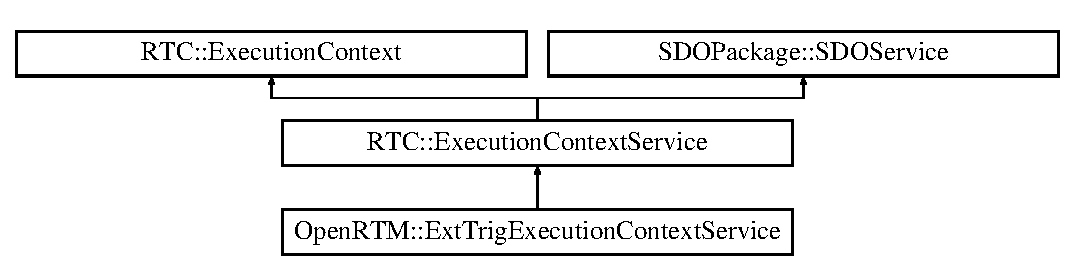
\includegraphics[height=3cm]{interfaceRTC_1_1ExecutionContextService}
\end{center}
\end{figure}
\subsection*{Public Member Functions}
\begin{DoxyCompactItemize}
\item 
{\bf ExecutionContextProfile} {\bf get\_\-profile} ()
\begin{DoxyCompactList}\small\item\em get\_\-profile \item\end{DoxyCompactList}\item 
boolean {\bf is\_\-running} ()
\begin{DoxyCompactList}\small\item\em is\_\-running \item\end{DoxyCompactList}\item 
{\bf ReturnCode\_\-t} {\bf start} ()
\begin{DoxyCompactList}\small\item\em start \item\end{DoxyCompactList}\item 
{\bf ReturnCode\_\-t} {\bf stop} ()
\begin{DoxyCompactList}\small\item\em stop \item\end{DoxyCompactList}\item 
double {\bf get\_\-rate} ()
\begin{DoxyCompactList}\small\item\em get\_\-rate \item\end{DoxyCompactList}\item 
{\bf ReturnCode\_\-t} {\bf set\_\-rate} (in double rate)
\begin{DoxyCompactList}\small\item\em set\_\-rate \item\end{DoxyCompactList}\item 
{\bf ReturnCode\_\-t} {\bf add\_\-component} (in {\bf LightweightRTObject} comp)
\begin{DoxyCompactList}\small\item\em add\_\-component \item\end{DoxyCompactList}\item 
{\bf ReturnCode\_\-t} {\bf remove\_\-component} (in {\bf LightweightRTObject} comp)
\begin{DoxyCompactList}\small\item\em remove\_\-component \item\end{DoxyCompactList}\item 
{\bf ReturnCode\_\-t} {\bf activate\_\-component} (in {\bf LightweightRTObject} comp)
\begin{DoxyCompactList}\small\item\em activate\_\-component \item\end{DoxyCompactList}\item 
{\bf ReturnCode\_\-t} {\bf deactivate\_\-component} (in {\bf LightweightRTObject} comp)
\begin{DoxyCompactList}\small\item\em deactivate\_\-component \item\end{DoxyCompactList}\item 
{\bf ReturnCode\_\-t} {\bf reset\_\-component} (in {\bf LightweightRTObject} comp)
\begin{DoxyCompactList}\small\item\em reset\_\-component \item\end{DoxyCompactList}\item 
{\bf LifeCycleState} {\bf get\_\-component\_\-state} (in {\bf LightweightRTObject} comp)
\begin{DoxyCompactList}\small\item\em get\_\-component\_\-state \item\end{DoxyCompactList}\item 
{\bf ExecutionKind} {\bf get\_\-kind} ()
\begin{DoxyCompactList}\small\item\em get\_\-kind \item\end{DoxyCompactList}\end{DoxyCompactItemize}


\subsection{Detailed Description}
\doxyref{ExecutionContextService}{p.}{interfaceRTC_1_1ExecutionContextService}. \subsection{Description}\label{namespaceRTC_Description}
An \doxyref{ExecutionContextService}{p.}{interfaceRTC_1_1ExecutionContextService} exposes an \doxyref{ExecutionContext}{p.}{interfaceRTC_1_1ExecutionContext} as an SDO service such that the context may be controlled remotely.\subsection{Semantics}\label{namespaceRTC_Semantics}
Depending on the implementation, this interface may itself be an execution context (that is, it may be passed to the operations of \doxyref{ComponentAction}{p.}{interfaceRTC_1_1ComponentAction}) or it may represent a remote execution context that is not of type \doxyref{ExecutionContextService}{p.}{interfaceRTC_1_1ExecutionContextService}. 

\subsection{Member Function Documentation}
\index{RTC::ExecutionContextService@{RTC::ExecutionContextService}!activate\_\-component@{activate\_\-component}}
\index{activate\_\-component@{activate\_\-component}!RTC::ExecutionContextService@{RTC::ExecutionContextService}}
\subsubsection[{activate\_\-component}]{\setlength{\rightskip}{0pt plus 5cm}{\bf ReturnCode\_\-t} RTC::ExecutionContext::activate\_\-component (in {\bf LightweightRTObject} {\em comp})\hspace{0.3cm}{\ttfamily  [inherited]}}\label{interfaceRTC_1_1ExecutionContext_af4a8aeab4a5e71e731b89556ef3e33e1}


activate\_\-component 

\subsection{Description}\label{namespaceRTC_Description}
The given participant \doxyref{RTC}{p.}{namespaceRTC} is Inactive and is therefore not being invoked according to the execution context��s execution kind. This operation shall cause the \doxyref{RTC}{p.}{namespaceRTC} to transition to the Active state such that it may subsequently be invoked in this execution context.\subsection{Semantics}\label{namespaceRTC_Semantics}
The callback on\_\-activate shall be called as a result of calling this operation. This operation shall not return until the callback has returned, and shall result in an error if the callback does. The following figure is a non-\/normative example sequence diagram for activate\_\-component.\subsection{Constraints}\label{interfaceRTC_1_1LightweightRTObject_Constraints}

\begin{DoxyItemize}
\item An execution context can only activate its participant components. If the given \doxyref{RTC}{p.}{namespaceRTC} is not participating in the execution context, this operation shall fail with ReturnCode\_\-t::BAD\_\-PARAMETER.
\end{DoxyItemize}


\begin{DoxyItemize}
\item An \doxyref{RTC}{p.}{namespaceRTC} that is in the Error state cannot be activated until after it has been reset. If the given \doxyref{RTC}{p.}{namespaceRTC} is in the Error state, this operation shall fail with ReturnCode\_\-t::PRECONDITION\_\-NOT\_\-MET.
\end{DoxyItemize}


\begin{DoxyItemize}
\item This operation shall fail with ReturnCode\_\-t::BAD\_\-PARAMETER if the given component is not in its Alive state. 
\end{DoxyItemize}\index{RTC::ExecutionContextService@{RTC::ExecutionContextService}!add\_\-component@{add\_\-component}}
\index{add\_\-component@{add\_\-component}!RTC::ExecutionContextService@{RTC::ExecutionContextService}}
\subsubsection[{add\_\-component}]{\setlength{\rightskip}{0pt plus 5cm}{\bf ReturnCode\_\-t} RTC::ExecutionContext::add\_\-component (in {\bf LightweightRTObject} {\em comp})\hspace{0.3cm}{\ttfamily  [inherited]}}\label{interfaceRTC_1_1ExecutionContext_a7ac1a5b9820e571153db730c9369b600}


add\_\-component 

\subsection{Description}\label{namespaceRTC_Description}
The operation causes the given \doxyref{RTC}{p.}{namespaceRTC} to begin participating in the execution context.\subsection{Semantics}\label{namespaceRTC_Semantics}
The newly added \doxyref{RTC}{p.}{namespaceRTC} will receive a call to LightweightRTComponent::attach\_\-context (see Section 5.2.2.2.5) and then enter the Inactive state.\subsection{Constraints}\label{interfaceRTC_1_1LightweightRTObject_Constraints}

\begin{DoxyItemize}
\item If the ExecutionKind of this context is PERIODIC, the \doxyref{RTC}{p.}{namespaceRTC} must be a data flow component (see Section 5.3.1.1). Otherwise, this operation shall fail with ReturnCode\_\-t::PRECONDITION\_\-NOT\_\-MET.
\end{DoxyItemize}


\begin{DoxyItemize}
\item If the ExecutionKind of this context is EVENT\_\-DRIVEN, the \doxyref{RTC}{p.}{namespaceRTC} must be an FSM participant (see Section 5.3.2.3). Otherwise, this operation shall fail with ReturnCode\_\-t::PRECONDITION\_\-NOT\_\-MET. 
\end{DoxyItemize}\index{RTC::ExecutionContextService@{RTC::ExecutionContextService}!deactivate\_\-component@{deactivate\_\-component}}
\index{deactivate\_\-component@{deactivate\_\-component}!RTC::ExecutionContextService@{RTC::ExecutionContextService}}
\subsubsection[{deactivate\_\-component}]{\setlength{\rightskip}{0pt plus 5cm}{\bf ReturnCode\_\-t} RTC::ExecutionContext::deactivate\_\-component (in {\bf LightweightRTObject} {\em comp})\hspace{0.3cm}{\ttfamily  [inherited]}}\label{interfaceRTC_1_1ExecutionContext_a82a23124035a957f2191b520a011e870}


deactivate\_\-component 

\subsection{Description}\label{namespaceRTC_Description}
The given \doxyref{RTC}{p.}{namespaceRTC} is Active in the execution context. Cause it to transition to the Inactive state such that it will not be subsequently invoked from the context unless and until it is activated again.\subsection{Semantics}\label{namespaceRTC_Semantics}
The callback on\_\-deactivate shall be called as a result of calling this operation. This operation shall not return until the callback has returned, and shall result in an error if the callback does. The following figure is a non-\/normative example sequence diagram for deactivate\_\-component.\subsection{Constraints}\label{interfaceRTC_1_1LightweightRTObject_Constraints}

\begin{DoxyItemize}
\item An execution context can only deactivate its participant components. If the given \doxyref{RTC}{p.}{namespaceRTC} is not participating in the execution context, this operation shall fail with ReturnCode\_\-t::BAD\_\-PARAMETER.
\end{DoxyItemize}


\begin{DoxyItemize}
\item This operation shall fail with ReturnCode\_\-t::BAD\_\-PARAMETER if the given component is not in its Alive state. 
\end{DoxyItemize}\index{RTC::ExecutionContextService@{RTC::ExecutionContextService}!get\_\-component\_\-state@{get\_\-component\_\-state}}
\index{get\_\-component\_\-state@{get\_\-component\_\-state}!RTC::ExecutionContextService@{RTC::ExecutionContextService}}
\subsubsection[{get\_\-component\_\-state}]{\setlength{\rightskip}{0pt plus 5cm}{\bf LifeCycleState} RTC::ExecutionContext::get\_\-component\_\-state (in {\bf LightweightRTObject} {\em comp})\hspace{0.3cm}{\ttfamily  [inherited]}}\label{interfaceRTC_1_1ExecutionContext_a51a0396327ec0bab96f06a246032fc84}


get\_\-component\_\-state 

\subsection{Description}\label{namespaceRTC_Description}
This operation shall report the LifeCycleState of the given participant \doxyref{RTC}{p.}{namespaceRTC}.\subsection{Constraints}\label{interfaceRTC_1_1LightweightRTObject_Constraints}

\begin{DoxyItemize}
\item The given \doxyref{RTC}{p.}{namespaceRTC} must be Alive.
\end{DoxyItemize}


\begin{DoxyItemize}
\item The given \doxyref{RTC}{p.}{namespaceRTC} must be a participant in the target execution context.
\end{DoxyItemize}


\begin{DoxyItemize}
\item The LifeCycleState returned by this operation shall be one of LifeCycleState::INACTIVE, ACTIVE, or ERROR. 
\end{DoxyItemize}\index{RTC::ExecutionContextService@{RTC::ExecutionContextService}!get\_\-kind@{get\_\-kind}}
\index{get\_\-kind@{get\_\-kind}!RTC::ExecutionContextService@{RTC::ExecutionContextService}}
\subsubsection[{get\_\-kind}]{\setlength{\rightskip}{0pt plus 5cm}{\bf ExecutionKind} RTC::ExecutionContext::get\_\-kind ()\hspace{0.3cm}{\ttfamily  [inherited]}}\label{interfaceRTC_1_1ExecutionContext_aa7175c37b85b78b90ea5468a4f1379b0}


get\_\-kind 

\subsection{Description}\label{namespaceRTC_Description}
This operation shall report the execution kind of the execution context. \index{RTC::ExecutionContextService@{RTC::ExecutionContextService}!get\_\-profile@{get\_\-profile}}
\index{get\_\-profile@{get\_\-profile}!RTC::ExecutionContextService@{RTC::ExecutionContextService}}
\subsubsection[{get\_\-profile}]{\setlength{\rightskip}{0pt plus 5cm}{\bf ExecutionContextProfile} RTC::ExecutionContextService::get\_\-profile ()}\label{interfaceRTC_1_1ExecutionContextService_a5cad2c38e1f1b7c61d5f345c9c49a193}


get\_\-profile 

\subsection{Description}\label{namespaceRTC_Description}
This operation provides a profile \char`\"{}descriptor\char`\"{} for the execution context. \index{RTC::ExecutionContextService@{RTC::ExecutionContextService}!get\_\-rate@{get\_\-rate}}
\index{get\_\-rate@{get\_\-rate}!RTC::ExecutionContextService@{RTC::ExecutionContextService}}
\subsubsection[{get\_\-rate}]{\setlength{\rightskip}{0pt plus 5cm}double RTC::ExecutionContext::get\_\-rate ()\hspace{0.3cm}{\ttfamily  [inherited]}}\label{interfaceRTC_1_1ExecutionContext_ad9c05f6e738c310f4ad5c686770fa5cc}


get\_\-rate 

\subsection{Description}\label{namespaceRTC_Description}
This operation shall return the rate (in hertz) at which its Active participating RTCs are being invoked.\subsection{Semantics}\label{namespaceRTC_Semantics}
An implementation is permitted to perform some periodic or quasi-\/periodic processing within an execution context with an ExecutionKind other than PERIODIC. In such a case, the result of this operation is implementation-\/defined. If no periodic processing of any kind is taking place within the context, this operation shall fail as described in Section 5.2.1.\subsection{Constraints}\label{interfaceRTC_1_1LightweightRTObject_Constraints}

\begin{DoxyItemize}
\item If the context has an ExecutionKind of PERIODIC, this operation shall return a rate greater than zero. 
\end{DoxyItemize}\index{RTC::ExecutionContextService@{RTC::ExecutionContextService}!is\_\-running@{is\_\-running}}
\index{is\_\-running@{is\_\-running}!RTC::ExecutionContextService@{RTC::ExecutionContextService}}
\subsubsection[{is\_\-running}]{\setlength{\rightskip}{0pt plus 5cm}boolean RTC::ExecutionContext::is\_\-running ()\hspace{0.3cm}{\ttfamily  [inherited]}}\label{interfaceRTC_1_1ExecutionContext_a4aa7b4668eccb0d88befaa411cf5283e}


is\_\-running 

\subsection{Description}\label{namespaceRTC_Description}
This operation shall return true if the context is in the Running state.\subsection{Semantics}\label{namespaceRTC_Semantics}
While the context is Running, all Active RTCs participating in the context shall be executed according to the context��s execution kind. \index{RTC::ExecutionContextService@{RTC::ExecutionContextService}!remove\_\-component@{remove\_\-component}}
\index{remove\_\-component@{remove\_\-component}!RTC::ExecutionContextService@{RTC::ExecutionContextService}}
\subsubsection[{remove\_\-component}]{\setlength{\rightskip}{0pt plus 5cm}{\bf ReturnCode\_\-t} RTC::ExecutionContext::remove\_\-component (in {\bf LightweightRTObject} {\em comp})\hspace{0.3cm}{\ttfamily  [inherited]}}\label{interfaceRTC_1_1ExecutionContext_a75d5152e03f4bfcf9a905aa0f9083243}


remove\_\-component 

\subsection{Description}\label{namespaceRTC_Description}
This operation causes a participant \doxyref{RTC}{p.}{namespaceRTC} to stop participating in the execution context.\subsection{Semantics}\label{namespaceRTC_Semantics}
The removed \doxyref{RTC}{p.}{namespaceRTC} will receive a call to LightweightRTComponent::detach\_\-context (see Section 5.2.2.2.6).\subsection{Constraints}\label{interfaceRTC_1_1LightweightRTObject_Constraints}

\begin{DoxyItemize}
\item If the given \doxyref{RTC}{p.}{namespaceRTC} is not currently participating in the execution context, this operation shall fail with ReturnCode\_\-t::BAD\_\-PARAMETER.
\end{DoxyItemize}


\begin{DoxyItemize}
\item An \doxyref{RTC}{p.}{namespaceRTC} must be deactivated before it can be removed from an execution context. If the given \doxyref{RTC}{p.}{namespaceRTC} is participating in the execution context but is still in the Active state, this operation shall fail with ReturnCode\_\-t::PRECONDITION\_\-NOT\_\-MET. 
\end{DoxyItemize}\index{RTC::ExecutionContextService@{RTC::ExecutionContextService}!reset\_\-component@{reset\_\-component}}
\index{reset\_\-component@{reset\_\-component}!RTC::ExecutionContextService@{RTC::ExecutionContextService}}
\subsubsection[{reset\_\-component}]{\setlength{\rightskip}{0pt plus 5cm}{\bf ReturnCode\_\-t} RTC::ExecutionContext::reset\_\-component (in {\bf LightweightRTObject} {\em comp})\hspace{0.3cm}{\ttfamily  [inherited]}}\label{interfaceRTC_1_1ExecutionContext_a27a1ae76eb00c58ba097a96fe358980b}


reset\_\-component 

\subsection{Description}\label{namespaceRTC_Description}
Attempt to recover the \doxyref{RTC}{p.}{namespaceRTC} when it is in Error.\subsection{Semantics}\label{namespaceRTC_Semantics}
The \doxyref{ComponentAction::on\_\-reset}{p.}{interfaceRTC_1_1ComponentAction_adb0e61bff251337d79c7c7d050d8304e} callback shall be invoked. This operation shall not return until the callback has returned, and shall result in an error if the callback does. If possible, the \doxyref{RTC}{p.}{namespaceRTC} developer should implement that callback such that the \doxyref{RTC}{p.}{namespaceRTC} may be returned to a valid state. $\ast$ If this operation fails, the \doxyref{RTC}{p.}{namespaceRTC} will remain in Error.\subsection{Constraints}\label{interfaceRTC_1_1LightweightRTObject_Constraints}

\begin{DoxyItemize}
\item An \doxyref{RTC}{p.}{namespaceRTC} may only be reset in an execution context in which it is in error. If the \doxyref{RTC}{p.}{namespaceRTC} is not in Error in the identified context, this operation shall fail with ReturnCode\_\-t::PRECONDITION\_\-NOT\_\-MET. However, that failure shall not cause the \doxyref{RTC}{p.}{namespaceRTC} to enter the Error state.
\end{DoxyItemize}


\begin{DoxyItemize}
\item An \doxyref{RTC}{p.}{namespaceRTC} may not be reset while in the Created state. Any attempt to invoke this operation while the \doxyref{RTC}{p.}{namespaceRTC} is in that state shall fail with ReturnCode\_\-t::PRECONDITION\_\-NOT\_\-MET. However, that failure shall not cause the \doxyref{RTC}{p.}{namespaceRTC} to enter the Error state. 
\end{DoxyItemize}\index{RTC::ExecutionContextService@{RTC::ExecutionContextService}!set\_\-rate@{set\_\-rate}}
\index{set\_\-rate@{set\_\-rate}!RTC::ExecutionContextService@{RTC::ExecutionContextService}}
\subsubsection[{set\_\-rate}]{\setlength{\rightskip}{0pt plus 5cm}{\bf ReturnCode\_\-t} RTC::ExecutionContext::set\_\-rate (in double {\em rate})\hspace{0.3cm}{\ttfamily  [inherited]}}\label{interfaceRTC_1_1ExecutionContext_ae6bdf760ff071970f9ed9e0a9d6fe459}


set\_\-rate 

\subsection{Description}\label{namespaceRTC_Description}
This operation shall set the rate (in hertz) at which this context��s Active participating RTCs are being called.\subsection{Semantics}\label{namespaceRTC_Semantics}
If the execution kind of the context is PERIODIC, a rate change shall result in the invocation of on\_\-rate\_\-changed on any RTCs realizing \doxyref{DataFlowComponentAction}{p.}{interfaceRTC_1_1DataFlowComponentAction} that are registered with any RTCs participating in the context. An implementation is permitted to perform some periodic or quasi-\/periodic processing within an execution context with an ExecutionKind other than PERIODIC. If such is the case, and the implementation reports a rate from get\_\-rate, this operation shall set that rate successfully provided that the given rate is valid. If no periodic processing of any kind is taking place within the context, this operation shall fail with ReturnCode\_\-t::UNSUPPORTED.\subsection{Constraints}\label{interfaceRTC_1_1LightweightRTObject_Constraints}

\begin{DoxyItemize}
\item The given rate must be greater than zero. Otherwise, this operation shall fail with ReturnCode\_\-t::BAD\_\-PARAMETER. 
\end{DoxyItemize}\index{RTC::ExecutionContextService@{RTC::ExecutionContextService}!start@{start}}
\index{start@{start}!RTC::ExecutionContextService@{RTC::ExecutionContextService}}
\subsubsection[{start}]{\setlength{\rightskip}{0pt plus 5cm}{\bf ReturnCode\_\-t} RTC::ExecutionContext::start ()\hspace{0.3cm}{\ttfamily  [inherited]}}\label{interfaceRTC_1_1ExecutionContext_ab015ee47c132e0cf223459d2db7b9f94}


start 

\subsection{Description}\label{namespaceRTC_Description}
Request that the context enter the Running state. Once the state transition occurs, the \doxyref{ComponentAction::on\_\-startup}{p.}{interfaceRTC_1_1ComponentAction_ac305f00c92f4650cf4fc798aac37eef2} operation (see Section 5.2.2.4.3) will be invoked. \subsection{Description}\label{namespaceRTC_Description}
\subsection{Semantics}\label{namespaceRTC_Semantics}
An execution context may not be started until the RT components that participate in it have been initialized. An execution context may be started and stopped multiple times.\subsection{Constraints}\label{interfaceRTC_1_1LightweightRTObject_Constraints}

\begin{DoxyItemize}
\item This operation shall fail with ReturnCode\_\-t::PRECONDITION\_\-NOT\_\-MET if the context is not in the Stopped state.
\end{DoxyItemize}


\begin{DoxyItemize}
\item This operation shall fail with ReturnCode\_\-t::PRECONDITION\_\-NOT\_\-MET if any of the participating components are not in their Alive state. 
\end{DoxyItemize}\index{RTC::ExecutionContextService@{RTC::ExecutionContextService}!stop@{stop}}
\index{stop@{stop}!RTC::ExecutionContextService@{RTC::ExecutionContextService}}
\subsubsection[{stop}]{\setlength{\rightskip}{0pt plus 5cm}{\bf ReturnCode\_\-t} RTC::ExecutionContext::stop ()\hspace{0.3cm}{\ttfamily  [inherited]}}\label{interfaceRTC_1_1ExecutionContext_afe216bae26d5817459a67e5b7e3134ce}


stop 

\subsection{Description}\label{namespaceRTC_Description}
Request that the context enter the Stopped state. Once the transition occurs, the \doxyref{ComponentAction::on\_\-shutdown}{p.}{interfaceRTC_1_1ComponentAction_accc47711344c811c9bdba0d66a3048f2} operation (see Section 5.2.2.4.4) will be invoked.\subsection{Semantics}\label{namespaceRTC_Semantics}
An execution context must be stopped before the RT components that participate in it are finalized.

An execution context may be started and stopped multiple times.\subsection{Constraints}\label{interfaceRTC_1_1LightweightRTObject_Constraints}

\begin{DoxyItemize}
\item This operation shall fail with ReturnCode\_\-t::PRECONDITION\_\-NOT\_\-MET if the context is not in the Running state. 
\end{DoxyItemize}

The documentation for this interface was generated from the following file:\begin{DoxyCompactItemize}
\item 
{\bf RTC.idl}\end{DoxyCompactItemize}

\section{OpenRTM::ExtTrigExecutionContextService Interface Reference}
\label{interfaceOpenRTM_1_1ExtTrigExecutionContextService}\index{OpenRTM::ExtTrigExecutionContextService@{OpenRTM::ExtTrigExecutionContextService}}


{\ttfamily import \char`\"{}OpenRTM.idl\char`\"{};}

Inheritance diagram for OpenRTM::ExtTrigExecutionContextService:\begin{figure}[H]
\begin{center}
\leavevmode
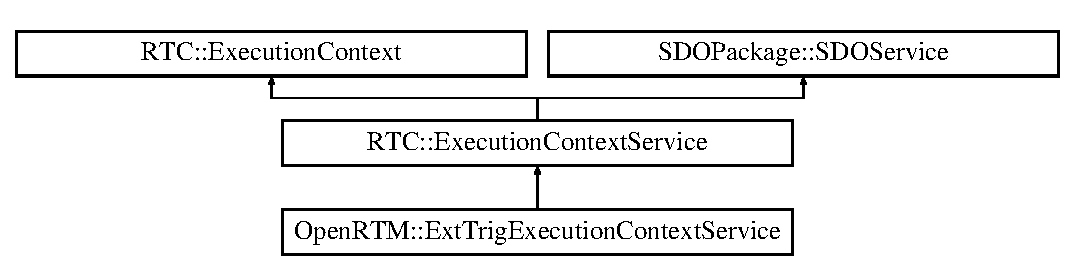
\includegraphics[height=3cm]{interfaceOpenRTM_1_1ExtTrigExecutionContextService}
\end{center}
\end{figure}
\subsection*{Public Member Functions}
\begin{DoxyCompactItemize}
\item 
void {\bf tick} ()
\item 
ExecutionContextProfile {\bf get\_\-profile} ()
\begin{DoxyCompactList}\small\item\em get\_\-profile \item\end{DoxyCompactList}\item 
boolean {\bf is\_\-running} ()
\begin{DoxyCompactList}\small\item\em is\_\-running \item\end{DoxyCompactList}\item 
ReturnCode\_\-t {\bf start} ()
\begin{DoxyCompactList}\small\item\em start \item\end{DoxyCompactList}\item 
ReturnCode\_\-t {\bf stop} ()
\begin{DoxyCompactList}\small\item\em stop \item\end{DoxyCompactList}\item 
double {\bf get\_\-rate} ()
\begin{DoxyCompactList}\small\item\em get\_\-rate \item\end{DoxyCompactList}\item 
ReturnCode\_\-t {\bf set\_\-rate} (in double rate)
\begin{DoxyCompactList}\small\item\em set\_\-rate \item\end{DoxyCompactList}\item 
ReturnCode\_\-t {\bf add\_\-component} (in LightweightRTObject comp)
\begin{DoxyCompactList}\small\item\em add\_\-component \item\end{DoxyCompactList}\item 
ReturnCode\_\-t {\bf remove\_\-component} (in LightweightRTObject comp)
\begin{DoxyCompactList}\small\item\em remove\_\-component \item\end{DoxyCompactList}\item 
ReturnCode\_\-t {\bf activate\_\-component} (in LightweightRTObject comp)
\begin{DoxyCompactList}\small\item\em activate\_\-component \item\end{DoxyCompactList}\item 
ReturnCode\_\-t {\bf deactivate\_\-component} (in LightweightRTObject comp)
\begin{DoxyCompactList}\small\item\em deactivate\_\-component \item\end{DoxyCompactList}\item 
ReturnCode\_\-t {\bf reset\_\-component} (in LightweightRTObject comp)
\begin{DoxyCompactList}\small\item\em reset\_\-component \item\end{DoxyCompactList}\item 
LifeCycleState {\bf get\_\-component\_\-state} (in LightweightRTObject comp)
\begin{DoxyCompactList}\small\item\em get\_\-component\_\-state \item\end{DoxyCompactList}\item 
ExecutionKind {\bf get\_\-kind} ()
\begin{DoxyCompactList}\small\item\em get\_\-kind \item\end{DoxyCompactList}\end{DoxyCompactItemize}


\subsection{Member Function Documentation}
\index{OpenRTM::ExtTrigExecutionContextService@{OpenRTM::ExtTrigExecutionContextService}!activate\_\-component@{activate\_\-component}}
\index{activate\_\-component@{activate\_\-component}!OpenRTM::ExtTrigExecutionContextService@{OpenRTM::ExtTrigExecutionContextService}}
\subsubsection[{activate\_\-component}]{\setlength{\rightskip}{0pt plus 5cm}ReturnCode\_\-t RTC::ExecutionContext::activate\_\-component (in {\bf LightweightRTObject} {\em comp})\hspace{0.3cm}{\ttfamily  [inherited]}}\label{interfaceRTC_1_1ExecutionContext_af4a8aeab4a5e71e731b89556ef3e33e1}


activate\_\-component 

\subsection{Description}\label{namespaceRTC_Description}
The given participant \doxyref{RTC}{p.}{namespaceRTC} is Inactive and is therefore not being invoked according to the execution context��s execution kind. This operation shall cause the \doxyref{RTC}{p.}{namespaceRTC} to transition to the Active state such that it may subsequently be invoked in this execution context.\subsection{Semantics}\label{namespaceRTC_Semantics}
The callback on\_\-activate shall be called as a result of calling this operation. This operation shall not return until the callback has returned, and shall result in an error if the callback does. The following figure is a non-\/normative example sequence diagram for activate\_\-component.\subsection{Constraints}\label{interfaceRTC_1_1LightweightRTObject_Constraints}

\begin{DoxyItemize}
\item An execution context can only activate its participant components. If the given \doxyref{RTC}{p.}{namespaceRTC} is not participating in the execution context, this operation shall fail with ReturnCode\_\-t::BAD\_\-PARAMETER.
\end{DoxyItemize}


\begin{DoxyItemize}
\item An \doxyref{RTC}{p.}{namespaceRTC} that is in the Error state cannot be activated until after it has been reset. If the given \doxyref{RTC}{p.}{namespaceRTC} is in the Error state, this operation shall fail with ReturnCode\_\-t::PRECONDITION\_\-NOT\_\-MET.
\end{DoxyItemize}


\begin{DoxyItemize}
\item This operation shall fail with ReturnCode\_\-t::BAD\_\-PARAMETER if the given component is not in its Alive state. 
\end{DoxyItemize}\index{OpenRTM::ExtTrigExecutionContextService@{OpenRTM::ExtTrigExecutionContextService}!add\_\-component@{add\_\-component}}
\index{add\_\-component@{add\_\-component}!OpenRTM::ExtTrigExecutionContextService@{OpenRTM::ExtTrigExecutionContextService}}
\subsubsection[{add\_\-component}]{\setlength{\rightskip}{0pt plus 5cm}ReturnCode\_\-t RTC::ExecutionContext::add\_\-component (in {\bf LightweightRTObject} {\em comp})\hspace{0.3cm}{\ttfamily  [inherited]}}\label{interfaceRTC_1_1ExecutionContext_a7ac1a5b9820e571153db730c9369b600}


add\_\-component 

\subsection{Description}\label{namespaceRTC_Description}
The operation causes the given \doxyref{RTC}{p.}{namespaceRTC} to begin participating in the execution context.\subsection{Semantics}\label{namespaceRTC_Semantics}
The newly added \doxyref{RTC}{p.}{namespaceRTC} will receive a call to LightweightRTComponent::attach\_\-context (see Section 5.2.2.2.5) and then enter the Inactive state.\subsection{Constraints}\label{interfaceRTC_1_1LightweightRTObject_Constraints}

\begin{DoxyItemize}
\item If the ExecutionKind of this context is PERIODIC, the \doxyref{RTC}{p.}{namespaceRTC} must be a data flow component (see Section 5.3.1.1). Otherwise, this operation shall fail with ReturnCode\_\-t::PRECONDITION\_\-NOT\_\-MET.
\end{DoxyItemize}


\begin{DoxyItemize}
\item If the ExecutionKind of this context is EVENT\_\-DRIVEN, the \doxyref{RTC}{p.}{namespaceRTC} must be an FSM participant (see Section 5.3.2.3). Otherwise, this operation shall fail with ReturnCode\_\-t::PRECONDITION\_\-NOT\_\-MET. 
\end{DoxyItemize}\index{OpenRTM::ExtTrigExecutionContextService@{OpenRTM::ExtTrigExecutionContextService}!deactivate\_\-component@{deactivate\_\-component}}
\index{deactivate\_\-component@{deactivate\_\-component}!OpenRTM::ExtTrigExecutionContextService@{OpenRTM::ExtTrigExecutionContextService}}
\subsubsection[{deactivate\_\-component}]{\setlength{\rightskip}{0pt plus 5cm}ReturnCode\_\-t RTC::ExecutionContext::deactivate\_\-component (in {\bf LightweightRTObject} {\em comp})\hspace{0.3cm}{\ttfamily  [inherited]}}\label{interfaceRTC_1_1ExecutionContext_a82a23124035a957f2191b520a011e870}


deactivate\_\-component 

\subsection{Description}\label{namespaceRTC_Description}
The given \doxyref{RTC}{p.}{namespaceRTC} is Active in the execution context. Cause it to transition to the Inactive state such that it will not be subsequently invoked from the context unless and until it is activated again.\subsection{Semantics}\label{namespaceRTC_Semantics}
The callback on\_\-deactivate shall be called as a result of calling this operation. This operation shall not return until the callback has returned, and shall result in an error if the callback does. The following figure is a non-\/normative example sequence diagram for deactivate\_\-component.\subsection{Constraints}\label{interfaceRTC_1_1LightweightRTObject_Constraints}

\begin{DoxyItemize}
\item An execution context can only deactivate its participant components. If the given \doxyref{RTC}{p.}{namespaceRTC} is not participating in the execution context, this operation shall fail with ReturnCode\_\-t::BAD\_\-PARAMETER.
\end{DoxyItemize}


\begin{DoxyItemize}
\item This operation shall fail with ReturnCode\_\-t::BAD\_\-PARAMETER if the given component is not in its Alive state. 
\end{DoxyItemize}\index{OpenRTM::ExtTrigExecutionContextService@{OpenRTM::ExtTrigExecutionContextService}!get\_\-component\_\-state@{get\_\-component\_\-state}}
\index{get\_\-component\_\-state@{get\_\-component\_\-state}!OpenRTM::ExtTrigExecutionContextService@{OpenRTM::ExtTrigExecutionContextService}}
\subsubsection[{get\_\-component\_\-state}]{\setlength{\rightskip}{0pt plus 5cm}LifeCycleState RTC::ExecutionContext::get\_\-component\_\-state (in {\bf LightweightRTObject} {\em comp})\hspace{0.3cm}{\ttfamily  [inherited]}}\label{interfaceRTC_1_1ExecutionContext_a51a0396327ec0bab96f06a246032fc84}


get\_\-component\_\-state 

\subsection{Description}\label{namespaceRTC_Description}
This operation shall report the LifeCycleState of the given participant \doxyref{RTC}{p.}{namespaceRTC}.\subsection{Constraints}\label{interfaceRTC_1_1LightweightRTObject_Constraints}

\begin{DoxyItemize}
\item The given \doxyref{RTC}{p.}{namespaceRTC} must be Alive.
\end{DoxyItemize}


\begin{DoxyItemize}
\item The given \doxyref{RTC}{p.}{namespaceRTC} must be a participant in the target execution context.
\end{DoxyItemize}


\begin{DoxyItemize}
\item The LifeCycleState returned by this operation shall be one of LifeCycleState::INACTIVE, ACTIVE, or ERROR. 
\end{DoxyItemize}\index{OpenRTM::ExtTrigExecutionContextService@{OpenRTM::ExtTrigExecutionContextService}!get\_\-kind@{get\_\-kind}}
\index{get\_\-kind@{get\_\-kind}!OpenRTM::ExtTrigExecutionContextService@{OpenRTM::ExtTrigExecutionContextService}}
\subsubsection[{get\_\-kind}]{\setlength{\rightskip}{0pt plus 5cm}ExecutionKind RTC::ExecutionContext::get\_\-kind ()\hspace{0.3cm}{\ttfamily  [inherited]}}\label{interfaceRTC_1_1ExecutionContext_aa7175c37b85b78b90ea5468a4f1379b0}


get\_\-kind 

\subsection{Description}\label{namespaceRTC_Description}
This operation shall report the execution kind of the execution context. \index{OpenRTM::ExtTrigExecutionContextService@{OpenRTM::ExtTrigExecutionContextService}!get\_\-profile@{get\_\-profile}}
\index{get\_\-profile@{get\_\-profile}!OpenRTM::ExtTrigExecutionContextService@{OpenRTM::ExtTrigExecutionContextService}}
\subsubsection[{get\_\-profile}]{\setlength{\rightskip}{0pt plus 5cm}ExecutionContextProfile RTC::ExecutionContextService::get\_\-profile ()\hspace{0.3cm}{\ttfamily  [inherited]}}\label{interfaceRTC_1_1ExecutionContextService_a5cad2c38e1f1b7c61d5f345c9c49a193}


get\_\-profile 

\subsection{Description}\label{namespaceRTC_Description}
This operation provides a profile \char`\"{}descriptor\char`\"{} for the execution context. \index{OpenRTM::ExtTrigExecutionContextService@{OpenRTM::ExtTrigExecutionContextService}!get\_\-rate@{get\_\-rate}}
\index{get\_\-rate@{get\_\-rate}!OpenRTM::ExtTrigExecutionContextService@{OpenRTM::ExtTrigExecutionContextService}}
\subsubsection[{get\_\-rate}]{\setlength{\rightskip}{0pt plus 5cm}double RTC::ExecutionContext::get\_\-rate ()\hspace{0.3cm}{\ttfamily  [inherited]}}\label{interfaceRTC_1_1ExecutionContext_ad9c05f6e738c310f4ad5c686770fa5cc}


get\_\-rate 

\subsection{Description}\label{namespaceRTC_Description}
This operation shall return the rate (in hertz) at which its Active participating RTCs are being invoked.\subsection{Semantics}\label{namespaceRTC_Semantics}
An implementation is permitted to perform some periodic or quasi-\/periodic processing within an execution context with an ExecutionKind other than PERIODIC. In such a case, the result of this operation is implementation-\/defined. If no periodic processing of any kind is taking place within the context, this operation shall fail as described in Section 5.2.1.\subsection{Constraints}\label{interfaceRTC_1_1LightweightRTObject_Constraints}

\begin{DoxyItemize}
\item If the context has an ExecutionKind of PERIODIC, this operation shall return a rate greater than zero. 
\end{DoxyItemize}\index{OpenRTM::ExtTrigExecutionContextService@{OpenRTM::ExtTrigExecutionContextService}!is\_\-running@{is\_\-running}}
\index{is\_\-running@{is\_\-running}!OpenRTM::ExtTrigExecutionContextService@{OpenRTM::ExtTrigExecutionContextService}}
\subsubsection[{is\_\-running}]{\setlength{\rightskip}{0pt plus 5cm}boolean RTC::ExecutionContext::is\_\-running ()\hspace{0.3cm}{\ttfamily  [inherited]}}\label{interfaceRTC_1_1ExecutionContext_a4aa7b4668eccb0d88befaa411cf5283e}


is\_\-running 

\subsection{Description}\label{namespaceRTC_Description}
This operation shall return true if the context is in the Running state.\subsection{Semantics}\label{namespaceRTC_Semantics}
While the context is Running, all Active RTCs participating in the context shall be executed according to the context��s execution kind. \index{OpenRTM::ExtTrigExecutionContextService@{OpenRTM::ExtTrigExecutionContextService}!remove\_\-component@{remove\_\-component}}
\index{remove\_\-component@{remove\_\-component}!OpenRTM::ExtTrigExecutionContextService@{OpenRTM::ExtTrigExecutionContextService}}
\subsubsection[{remove\_\-component}]{\setlength{\rightskip}{0pt plus 5cm}ReturnCode\_\-t RTC::ExecutionContext::remove\_\-component (in {\bf LightweightRTObject} {\em comp})\hspace{0.3cm}{\ttfamily  [inherited]}}\label{interfaceRTC_1_1ExecutionContext_a75d5152e03f4bfcf9a905aa0f9083243}


remove\_\-component 

\subsection{Description}\label{namespaceRTC_Description}
This operation causes a participant \doxyref{RTC}{p.}{namespaceRTC} to stop participating in the execution context.\subsection{Semantics}\label{namespaceRTC_Semantics}
The removed \doxyref{RTC}{p.}{namespaceRTC} will receive a call to LightweightRTComponent::detach\_\-context (see Section 5.2.2.2.6).\subsection{Constraints}\label{interfaceRTC_1_1LightweightRTObject_Constraints}

\begin{DoxyItemize}
\item If the given \doxyref{RTC}{p.}{namespaceRTC} is not currently participating in the execution context, this operation shall fail with ReturnCode\_\-t::BAD\_\-PARAMETER.
\end{DoxyItemize}


\begin{DoxyItemize}
\item An \doxyref{RTC}{p.}{namespaceRTC} must be deactivated before it can be removed from an execution context. If the given \doxyref{RTC}{p.}{namespaceRTC} is participating in the execution context but is still in the Active state, this operation shall fail with ReturnCode\_\-t::PRECONDITION\_\-NOT\_\-MET. 
\end{DoxyItemize}\index{OpenRTM::ExtTrigExecutionContextService@{OpenRTM::ExtTrigExecutionContextService}!reset\_\-component@{reset\_\-component}}
\index{reset\_\-component@{reset\_\-component}!OpenRTM::ExtTrigExecutionContextService@{OpenRTM::ExtTrigExecutionContextService}}
\subsubsection[{reset\_\-component}]{\setlength{\rightskip}{0pt plus 5cm}ReturnCode\_\-t RTC::ExecutionContext::reset\_\-component (in {\bf LightweightRTObject} {\em comp})\hspace{0.3cm}{\ttfamily  [inherited]}}\label{interfaceRTC_1_1ExecutionContext_a27a1ae76eb00c58ba097a96fe358980b}


reset\_\-component 

\subsection{Description}\label{namespaceRTC_Description}
Attempt to recover the \doxyref{RTC}{p.}{namespaceRTC} when it is in Error.\subsection{Semantics}\label{namespaceRTC_Semantics}
The \doxyref{ComponentAction::on\_\-reset}{p.}{interfaceRTC_1_1ComponentAction_adb0e61bff251337d79c7c7d050d8304e} callback shall be invoked. This operation shall not return until the callback has returned, and shall result in an error if the callback does. If possible, the \doxyref{RTC}{p.}{namespaceRTC} developer should implement that callback such that the \doxyref{RTC}{p.}{namespaceRTC} may be returned to a valid state. $\ast$ If this operation fails, the \doxyref{RTC}{p.}{namespaceRTC} will remain in Error.\subsection{Constraints}\label{interfaceRTC_1_1LightweightRTObject_Constraints}

\begin{DoxyItemize}
\item An \doxyref{RTC}{p.}{namespaceRTC} may only be reset in an execution context in which it is in error. If the \doxyref{RTC}{p.}{namespaceRTC} is not in Error in the identified context, this operation shall fail with ReturnCode\_\-t::PRECONDITION\_\-NOT\_\-MET. However, that failure shall not cause the \doxyref{RTC}{p.}{namespaceRTC} to enter the Error state.
\end{DoxyItemize}


\begin{DoxyItemize}
\item An \doxyref{RTC}{p.}{namespaceRTC} may not be reset while in the Created state. Any attempt to invoke this operation while the \doxyref{RTC}{p.}{namespaceRTC} is in that state shall fail with ReturnCode\_\-t::PRECONDITION\_\-NOT\_\-MET. However, that failure shall not cause the \doxyref{RTC}{p.}{namespaceRTC} to enter the Error state. 
\end{DoxyItemize}\index{OpenRTM::ExtTrigExecutionContextService@{OpenRTM::ExtTrigExecutionContextService}!set\_\-rate@{set\_\-rate}}
\index{set\_\-rate@{set\_\-rate}!OpenRTM::ExtTrigExecutionContextService@{OpenRTM::ExtTrigExecutionContextService}}
\subsubsection[{set\_\-rate}]{\setlength{\rightskip}{0pt plus 5cm}ReturnCode\_\-t RTC::ExecutionContext::set\_\-rate (in double {\em rate})\hspace{0.3cm}{\ttfamily  [inherited]}}\label{interfaceRTC_1_1ExecutionContext_ae6bdf760ff071970f9ed9e0a9d6fe459}


set\_\-rate 

\subsection{Description}\label{namespaceRTC_Description}
This operation shall set the rate (in hertz) at which this context��s Active participating RTCs are being called.\subsection{Semantics}\label{namespaceRTC_Semantics}
If the execution kind of the context is PERIODIC, a rate change shall result in the invocation of on\_\-rate\_\-changed on any RTCs realizing \doxyref{DataFlowComponentAction}{p.}{interfaceRTC_1_1DataFlowComponentAction} that are registered with any RTCs participating in the context. An implementation is permitted to perform some periodic or quasi-\/periodic processing within an execution context with an ExecutionKind other than PERIODIC. If such is the case, and the implementation reports a rate from get\_\-rate, this operation shall set that rate successfully provided that the given rate is valid. If no periodic processing of any kind is taking place within the context, this operation shall fail with ReturnCode\_\-t::UNSUPPORTED.\subsection{Constraints}\label{interfaceRTC_1_1LightweightRTObject_Constraints}

\begin{DoxyItemize}
\item The given rate must be greater than zero. Otherwise, this operation shall fail with ReturnCode\_\-t::BAD\_\-PARAMETER. 
\end{DoxyItemize}\index{OpenRTM::ExtTrigExecutionContextService@{OpenRTM::ExtTrigExecutionContextService}!start@{start}}
\index{start@{start}!OpenRTM::ExtTrigExecutionContextService@{OpenRTM::ExtTrigExecutionContextService}}
\subsubsection[{start}]{\setlength{\rightskip}{0pt plus 5cm}ReturnCode\_\-t RTC::ExecutionContext::start ()\hspace{0.3cm}{\ttfamily  [inherited]}}\label{interfaceRTC_1_1ExecutionContext_ab015ee47c132e0cf223459d2db7b9f94}


start 

\subsection{Description}\label{namespaceRTC_Description}
Request that the context enter the Running state. Once the state transition occurs, the \doxyref{ComponentAction::on\_\-startup}{p.}{interfaceRTC_1_1ComponentAction_ac305f00c92f4650cf4fc798aac37eef2} operation (see Section 5.2.2.4.3) will be invoked. \subsection{Description}\label{namespaceRTC_Description}
\subsection{Semantics}\label{namespaceRTC_Semantics}
An execution context may not be started until the RT components that participate in it have been initialized. An execution context may be started and stopped multiple times.\subsection{Constraints}\label{interfaceRTC_1_1LightweightRTObject_Constraints}

\begin{DoxyItemize}
\item This operation shall fail with ReturnCode\_\-t::PRECONDITION\_\-NOT\_\-MET if the context is not in the Stopped state.
\end{DoxyItemize}


\begin{DoxyItemize}
\item This operation shall fail with ReturnCode\_\-t::PRECONDITION\_\-NOT\_\-MET if any of the participating components are not in their Alive state. 
\end{DoxyItemize}\index{OpenRTM::ExtTrigExecutionContextService@{OpenRTM::ExtTrigExecutionContextService}!stop@{stop}}
\index{stop@{stop}!OpenRTM::ExtTrigExecutionContextService@{OpenRTM::ExtTrigExecutionContextService}}
\subsubsection[{stop}]{\setlength{\rightskip}{0pt plus 5cm}ReturnCode\_\-t RTC::ExecutionContext::stop ()\hspace{0.3cm}{\ttfamily  [inherited]}}\label{interfaceRTC_1_1ExecutionContext_afe216bae26d5817459a67e5b7e3134ce}


stop 

\subsection{Description}\label{namespaceRTC_Description}
Request that the context enter the Stopped state. Once the transition occurs, the \doxyref{ComponentAction::on\_\-shutdown}{p.}{interfaceRTC_1_1ComponentAction_accc47711344c811c9bdba0d66a3048f2} operation (see Section 5.2.2.4.4) will be invoked.\subsection{Semantics}\label{namespaceRTC_Semantics}
An execution context must be stopped before the RT components that participate in it are finalized.

An execution context may be started and stopped multiple times.\subsection{Constraints}\label{interfaceRTC_1_1LightweightRTObject_Constraints}

\begin{DoxyItemize}
\item This operation shall fail with ReturnCode\_\-t::PRECONDITION\_\-NOT\_\-MET if the context is not in the Running state. 
\end{DoxyItemize}\index{OpenRTM::ExtTrigExecutionContextService@{OpenRTM::ExtTrigExecutionContextService}!tick@{tick}}
\index{tick@{tick}!OpenRTM::ExtTrigExecutionContextService@{OpenRTM::ExtTrigExecutionContextService}}
\subsubsection[{tick}]{\setlength{\rightskip}{0pt plus 5cm}void OpenRTM::ExtTrigExecutionContextService::tick ()}\label{interfaceOpenRTM_1_1ExtTrigExecutionContextService_a0a9227a44b63a0fc49fbc8ea9acc898d}


The documentation for this interface was generated from the following file:\begin{DoxyCompactItemize}
\item 
{\bf OpenRTM.idl}\end{DoxyCompactItemize}

\section{インタフェース RTC::Fsm}
\label{interfaceRTC_1_1Fsm}\index{RTC::Fsm@{RTC::Fsm}}


{\ttfamily import \char`\"{}RTC.idl\char`\"{};}

RTC::Fsmに対する継承グラフ\begin{figure}[H]
\begin{center}
\leavevmode
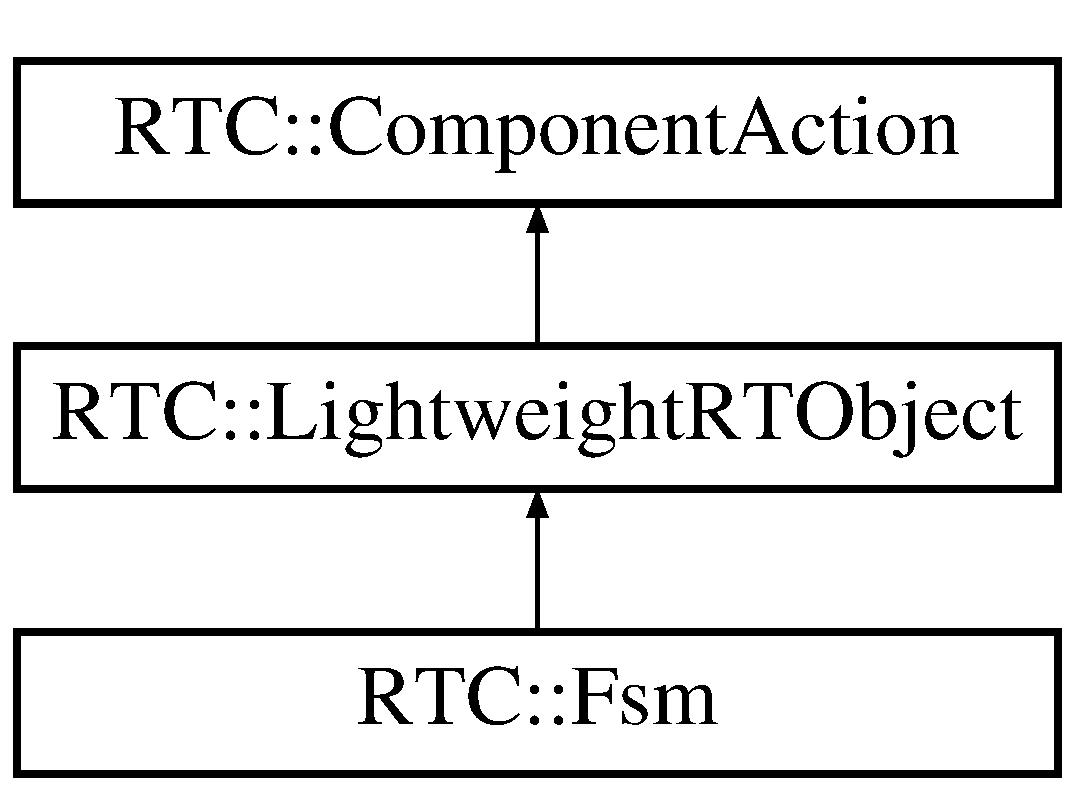
\includegraphics[height=3cm]{interfaceRTC_1_1Fsm}
\end{center}
\end{figure}
\subsection*{Public メソッド}
\begin{DoxyCompactItemize}
\item 
{\bf ReturnCode\_\-t} {\bf initialize} ()
\item 
{\bf ReturnCode\_\-t} {\bf finalize} ()
\item 
boolean {\bf is\_\-alive} (in {\bf ExecutionContext} exec\_\-context)
\item 
{\bf ReturnCode\_\-t} {\bf exit} ()
\item 
{\bf ExecutionContextHandle\_\-t} {\bf attach\_\-context} (in {\bf ExecutionContext} exec\_\-context)
\item 
{\bf ReturnCode\_\-t} {\bf detach\_\-context} (in {\bf ExecutionContextHandle\_\-t} exec\_\-handle)
\item 
{\bf ExecutionContext} {\bf get\_\-context} (in {\bf ExecutionContextHandle\_\-t} exec\_\-handle)
\item 
{\bf ExecutionContextList} {\bf get\_\-owned\_\-contexts} ()
\begin{DoxyCompactList}\small\item\em get\_\-owned\_\-contexts \item\end{DoxyCompactList}\item 
{\bf ExecutionContextList} {\bf get\_\-participating\_\-contexts} ()
\begin{DoxyCompactList}\small\item\em get\_\-participating\_\-contexts \item\end{DoxyCompactList}\item 
{\bf ExecutionContextHandle\_\-t} {\bf get\_\-context\_\-handle} (in {\bf ExecutionContext} cxt)
\item 
{\bf ReturnCode\_\-t} {\bf on\_\-initialize} ()
\item 
{\bf ReturnCode\_\-t} {\bf on\_\-finalize} ()
\item 
{\bf ReturnCode\_\-t} {\bf on\_\-startup} (in {\bf ExecutionContextHandle\_\-t} exec\_\-handle)
\item 
{\bf ReturnCode\_\-t} {\bf on\_\-shutdown} (in {\bf ExecutionContextHandle\_\-t} exec\_\-handle)
\item 
{\bf ReturnCode\_\-t} {\bf on\_\-activated} (in {\bf ExecutionContextHandle\_\-t} exec\_\-handle)
\item 
{\bf ReturnCode\_\-t} {\bf on\_\-deactivated} (in {\bf ExecutionContextHandle\_\-t} exec\_\-handle)
\item 
{\bf ReturnCode\_\-t} {\bf on\_\-aborting} (in {\bf ExecutionContextHandle\_\-t} exec\_\-handle)
\item 
{\bf ReturnCode\_\-t} {\bf on\_\-error} (in {\bf ExecutionContextHandle\_\-t} exec\_\-handle)
\item 
{\bf ReturnCode\_\-t} {\bf on\_\-reset} (in {\bf ExecutionContextHandle\_\-t} exec\_\-handle)
\end{DoxyCompactItemize}


\subsection{関数}
\index{RTC::Fsm@{RTC::Fsm}!attach\_\-context@{attach\_\-context}}
\index{attach\_\-context@{attach\_\-context}!RTC::Fsm@{RTC::Fsm}}
\subsubsection[{attach\_\-context}]{\setlength{\rightskip}{0pt plus 5cm}{\bf ExecutionContextHandle\_\-t} RTC::LightweightRTObject::attach\_\-context (in {\bf ExecutionContext} {\em exec\_\-context})\hspace{0.3cm}{\ttfamily  [inherited]}}\label{interfaceRTC_1_1LightweightRTObject_a48dbdbcac3254c29ad01d43a4ee5a00c}
\index{RTC::Fsm@{RTC::Fsm}!detach\_\-context@{detach\_\-context}}
\index{detach\_\-context@{detach\_\-context}!RTC::Fsm@{RTC::Fsm}}
\subsubsection[{detach\_\-context}]{\setlength{\rightskip}{0pt plus 5cm}{\bf ReturnCode\_\-t} RTC::LightweightRTObject::detach\_\-context (in {\bf ExecutionContextHandle\_\-t} {\em exec\_\-handle})\hspace{0.3cm}{\ttfamily  [inherited]}}\label{interfaceRTC_1_1LightweightRTObject_a8eb94420ca08e8f7acaa778ed883b9a4}
\index{RTC::Fsm@{RTC::Fsm}!exit@{exit}}
\index{exit@{exit}!RTC::Fsm@{RTC::Fsm}}
\subsubsection[{exit}]{\setlength{\rightskip}{0pt plus 5cm}{\bf ReturnCode\_\-t} RTC::LightweightRTObject::exit ()\hspace{0.3cm}{\ttfamily  [inherited]}}\label{interfaceRTC_1_1LightweightRTObject_a49bd940b6964fa80d696db15b45c2f87}
\index{RTC::Fsm@{RTC::Fsm}!finalize@{finalize}}
\index{finalize@{finalize}!RTC::Fsm@{RTC::Fsm}}
\subsubsection[{finalize}]{\setlength{\rightskip}{0pt plus 5cm}{\bf ReturnCode\_\-t} RTC::LightweightRTObject::finalize ()\hspace{0.3cm}{\ttfamily  [inherited]}}\label{interfaceRTC_1_1LightweightRTObject_a23466f177b4289662ea035be831426ad}
\index{RTC::Fsm@{RTC::Fsm}!get\_\-context@{get\_\-context}}
\index{get\_\-context@{get\_\-context}!RTC::Fsm@{RTC::Fsm}}
\subsubsection[{get\_\-context}]{\setlength{\rightskip}{0pt plus 5cm}{\bf ExecutionContext} RTC::LightweightRTObject::get\_\-context (in {\bf ExecutionContextHandle\_\-t} {\em exec\_\-handle})\hspace{0.3cm}{\ttfamily  [inherited]}}\label{interfaceRTC_1_1LightweightRTObject_a7bb123faf81bcb57542c3a17f10948d6}
\index{RTC::Fsm@{RTC::Fsm}!get\_\-context\_\-handle@{get\_\-context\_\-handle}}
\index{get\_\-context\_\-handle@{get\_\-context\_\-handle}!RTC::Fsm@{RTC::Fsm}}
\subsubsection[{get\_\-context\_\-handle}]{\setlength{\rightskip}{0pt plus 5cm}{\bf ExecutionContextHandle\_\-t} RTC::LightweightRTObject::get\_\-context\_\-handle (in {\bf ExecutionContext} {\em cxt})\hspace{0.3cm}{\ttfamily  [inherited]}}\label{interfaceRTC_1_1LightweightRTObject_af54041744c01d68026aa200276e12f45}
\#\#\# [����] \doxyref{RTC.idl}{p.}{RTC_8idl} �ˤϴޤޤ�Ƥ��ʤ���PIM�ˤϴޤޤ�Ƥ��롣 \#\#\# PIM���������� \index{RTC::Fsm@{RTC::Fsm}!get\_\-owned\_\-contexts@{get\_\-owned\_\-contexts}}
\index{get\_\-owned\_\-contexts@{get\_\-owned\_\-contexts}!RTC::Fsm@{RTC::Fsm}}
\subsubsection[{get\_\-owned\_\-contexts}]{\setlength{\rightskip}{0pt plus 5cm}{\bf ExecutionContextList} RTC::LightweightRTObject::get\_\-owned\_\-contexts ()\hspace{0.3cm}{\ttfamily  [inherited]}}\label{interfaceRTC_1_1LightweightRTObject_aea9dd2a447cc3ddc55f20aab698da408}


get\_\-owned\_\-contexts 

\subsection{Description}\label{interfaceRTC_1_1LightweightRTObject_Description}
���� \doxyref{RTC}{p.}{namespaceRTC} ����ͭ���� \doxyref{ExecutionContext}{p.}{interfaceRTC_1_1ExecutionContext} �Υꥹ�Ȥ�������롣 \index{RTC::Fsm@{RTC::Fsm}!get\_\-participating\_\-contexts@{get\_\-participating\_\-contexts}}
\index{get\_\-participating\_\-contexts@{get\_\-participating\_\-contexts}!RTC::Fsm@{RTC::Fsm}}
\subsubsection[{get\_\-participating\_\-contexts}]{\setlength{\rightskip}{0pt plus 5cm}{\bf ExecutionContextList} RTC::LightweightRTObject::get\_\-participating\_\-contexts ()\hspace{0.3cm}{\ttfamily  [inherited]}}\label{interfaceRTC_1_1LightweightRTObject_af2224880b89275ecf82efad0999b022a}


get\_\-participating\_\-contexts 

\subsection{Description}\label{interfaceRTC_1_1LightweightRTObject_Description}
���� \doxyref{RTC}{p.}{namespaceRTC} �����ä��Ƥ��뤹�٤Ƥ� \doxyref{ExecutionContext}{p.}{interfaceRTC_1_1ExecutionContext} �Υꥹ�Ȥ�������롣\subsection{Semantics}\label{interfaceRTC_1_1LightweightRTObject_Semantics}
���Υꥹ�Ȥ˴ޤޤ��¹ԥ���ƥ����Ȥϡ�attach\_\-context ���Ƥӽ� ����뤴�Ȥˡ��ꥹ�Ȥ��ɲä��졢detach\_\-context ���ƤӽФ���뤴 �Ȥˡ��ꥹ�Ȥ���������롣 \index{RTC::Fsm@{RTC::Fsm}!initialize@{initialize}}
\index{initialize@{initialize}!RTC::Fsm@{RTC::Fsm}}
\subsubsection[{initialize}]{\setlength{\rightskip}{0pt plus 5cm}{\bf ReturnCode\_\-t} RTC::LightweightRTObject::initialize ()\hspace{0.3cm}{\ttfamily  [inherited]}}\label{interfaceRTC_1_1LightweightRTObject_afb28c4d97677804da09488578b840eb5}
\index{RTC::Fsm@{RTC::Fsm}!is\_\-alive@{is\_\-alive}}
\index{is\_\-alive@{is\_\-alive}!RTC::Fsm@{RTC::Fsm}}
\subsubsection[{is\_\-alive}]{\setlength{\rightskip}{0pt plus 5cm}boolean RTC::LightweightRTObject::is\_\-alive (in {\bf ExecutionContext} {\em exec\_\-context})\hspace{0.3cm}{\ttfamily  [inherited]}}\label{interfaceRTC_1_1LightweightRTObject_aa07c8c299b0addc49887508c1ee7be27}
\index{RTC::Fsm@{RTC::Fsm}!on\_\-aborting@{on\_\-aborting}}
\index{on\_\-aborting@{on\_\-aborting}!RTC::Fsm@{RTC::Fsm}}
\subsubsection[{on\_\-aborting}]{\setlength{\rightskip}{0pt plus 5cm}{\bf ReturnCode\_\-t} RTC::ComponentAction::on\_\-aborting (in {\bf ExecutionContextHandle\_\-t} {\em exec\_\-handle})\hspace{0.3cm}{\ttfamily  [inherited]}}\label{interfaceRTC_1_1ComponentAction_a876e58ebcea16c307e131b3e6a58ddbe}
\index{RTC::Fsm@{RTC::Fsm}!on\_\-activated@{on\_\-activated}}
\index{on\_\-activated@{on\_\-activated}!RTC::Fsm@{RTC::Fsm}}
\subsubsection[{on\_\-activated}]{\setlength{\rightskip}{0pt plus 5cm}{\bf ReturnCode\_\-t} RTC::ComponentAction::on\_\-activated (in {\bf ExecutionContextHandle\_\-t} {\em exec\_\-handle})\hspace{0.3cm}{\ttfamily  [inherited]}}\label{interfaceRTC_1_1ComponentAction_a4f51f627067d0c54e89c4c0827fa6432}
\index{RTC::Fsm@{RTC::Fsm}!on\_\-deactivated@{on\_\-deactivated}}
\index{on\_\-deactivated@{on\_\-deactivated}!RTC::Fsm@{RTC::Fsm}}
\subsubsection[{on\_\-deactivated}]{\setlength{\rightskip}{0pt plus 5cm}{\bf ReturnCode\_\-t} RTC::ComponentAction::on\_\-deactivated (in {\bf ExecutionContextHandle\_\-t} {\em exec\_\-handle})\hspace{0.3cm}{\ttfamily  [inherited]}}\label{interfaceRTC_1_1ComponentAction_aa5f9cfb9677ba685be333ad666c87f88}
\index{RTC::Fsm@{RTC::Fsm}!on\_\-error@{on\_\-error}}
\index{on\_\-error@{on\_\-error}!RTC::Fsm@{RTC::Fsm}}
\subsubsection[{on\_\-error}]{\setlength{\rightskip}{0pt plus 5cm}{\bf ReturnCode\_\-t} RTC::ComponentAction::on\_\-error (in {\bf ExecutionContextHandle\_\-t} {\em exec\_\-handle})\hspace{0.3cm}{\ttfamily  [inherited]}}\label{interfaceRTC_1_1ComponentAction_a110fdde803e9b13f27308b897439962a}
\index{RTC::Fsm@{RTC::Fsm}!on\_\-finalize@{on\_\-finalize}}
\index{on\_\-finalize@{on\_\-finalize}!RTC::Fsm@{RTC::Fsm}}
\subsubsection[{on\_\-finalize}]{\setlength{\rightskip}{0pt plus 5cm}{\bf ReturnCode\_\-t} RTC::ComponentAction::on\_\-finalize ()\hspace{0.3cm}{\ttfamily  [inherited]}}\label{interfaceRTC_1_1ComponentAction_a9c9e2d638cd2b748609be8a23410aedc}
\index{RTC::Fsm@{RTC::Fsm}!on\_\-initialize@{on\_\-initialize}}
\index{on\_\-initialize@{on\_\-initialize}!RTC::Fsm@{RTC::Fsm}}
\subsubsection[{on\_\-initialize}]{\setlength{\rightskip}{0pt plus 5cm}{\bf ReturnCode\_\-t} RTC::ComponentAction::on\_\-initialize ()\hspace{0.3cm}{\ttfamily  [inherited]}}\label{interfaceRTC_1_1ComponentAction_a8703b183bc1bed9e2fd3ecac126cb231}
\index{RTC::Fsm@{RTC::Fsm}!on\_\-reset@{on\_\-reset}}
\index{on\_\-reset@{on\_\-reset}!RTC::Fsm@{RTC::Fsm}}
\subsubsection[{on\_\-reset}]{\setlength{\rightskip}{0pt plus 5cm}{\bf ReturnCode\_\-t} RTC::ComponentAction::on\_\-reset (in {\bf ExecutionContextHandle\_\-t} {\em exec\_\-handle})\hspace{0.3cm}{\ttfamily  [inherited]}}\label{interfaceRTC_1_1ComponentAction_adb0e61bff251337d79c7c7d050d8304e}
\index{RTC::Fsm@{RTC::Fsm}!on\_\-shutdown@{on\_\-shutdown}}
\index{on\_\-shutdown@{on\_\-shutdown}!RTC::Fsm@{RTC::Fsm}}
\subsubsection[{on\_\-shutdown}]{\setlength{\rightskip}{0pt plus 5cm}{\bf ReturnCode\_\-t} RTC::ComponentAction::on\_\-shutdown (in {\bf ExecutionContextHandle\_\-t} {\em exec\_\-handle})\hspace{0.3cm}{\ttfamily  [inherited]}}\label{interfaceRTC_1_1ComponentAction_accc47711344c811c9bdba0d66a3048f2}
\index{RTC::Fsm@{RTC::Fsm}!on\_\-startup@{on\_\-startup}}
\index{on\_\-startup@{on\_\-startup}!RTC::Fsm@{RTC::Fsm}}
\subsubsection[{on\_\-startup}]{\setlength{\rightskip}{0pt plus 5cm}{\bf ReturnCode\_\-t} RTC::ComponentAction::on\_\-startup (in {\bf ExecutionContextHandle\_\-t} {\em exec\_\-handle})\hspace{0.3cm}{\ttfamily  [inherited]}}\label{interfaceRTC_1_1ComponentAction_ac305f00c92f4650cf4fc798aac37eef2}


このインタフェースの説明は次のファイルから生成されました:\begin{DoxyCompactItemize}
\item 
{\bf RTC.idl}\end{DoxyCompactItemize}

\section{RTC::FsmBehaviorProfile Struct Reference}
\label{structRTC_1_1FsmBehaviorProfile}\index{RTC::FsmBehaviorProfile@{RTC::FsmBehaviorProfile}}


\doxyref{FsmBehaviorProfile}{p.}{structRTC_1_1FsmBehaviorProfile}.  




{\ttfamily import \char`\"{}RTC.idl\char`\"{};}

\subsection*{Public Attributes}
\begin{DoxyCompactItemize}
\item 
{\bf FsmParticipantAction} {\bf action\_\-component}
\begin{DoxyCompactList}\small\item\em action\_\-component \item\end{DoxyCompactList}\item 
{\bf UniqueIdentifier} {\bf id}
\begin{DoxyCompactList}\small\item\em id \item\end{DoxyCompactList}\end{DoxyCompactItemize}


\subsection{Detailed Description}
\doxyref{FsmBehaviorProfile}{p.}{structRTC_1_1FsmBehaviorProfile}. \subsection{Description}\label{namespaceRTC_Description}
\doxyref{FsmBehaviorProfile}{p.}{structRTC_1_1FsmBehaviorProfile} represents the association of an FSM participant with a transition, state entry, or state exit in an FSM.\subsection{Semantics}\label{namespaceRTC_Semantics}
The assignment of identifiers to particular transitions, state entries, or state exits is implementation-\/dependent. 

\subsection{Member Data Documentation}
\index{RTC::FsmBehaviorProfile@{RTC::FsmBehaviorProfile}!action\_\-component@{action\_\-component}}
\index{action\_\-component@{action\_\-component}!RTC::FsmBehaviorProfile@{RTC::FsmBehaviorProfile}}
\subsubsection[{action\_\-component}]{\setlength{\rightskip}{0pt plus 5cm}{\bf FsmParticipantAction} {\bf RTC::FsmBehaviorProfile::action\_\-component}}\label{structRTC_1_1FsmBehaviorProfile_acade0f218ed2bda5766f29609b35f3b6}


action\_\-component 

\subsection{Description}\label{namespaceRTC_Description}
This attribute stores a reference to the FSM participant that is invoked when the containing \doxyref{Fsm}{p.}{interfaceRTC_1_1Fsm} receives a message distinguished by id. \index{RTC::FsmBehaviorProfile@{RTC::FsmBehaviorProfile}!id@{id}}
\index{id@{id}!RTC::FsmBehaviorProfile@{RTC::FsmBehaviorProfile}}
\subsubsection[{id}]{\setlength{\rightskip}{0pt plus 5cm}{\bf UniqueIdentifier} {\bf RTC::FsmBehaviorProfile::id}}\label{structRTC_1_1FsmBehaviorProfile_a6b2f6efca3063fd7bbdea7a934aaec60}


id 

\subsection{Description}\label{namespaceRTC_Description}
This attribute stores the message identifier. 

The documentation for this struct was generated from the following file:\begin{DoxyCompactItemize}
\item 
{\bf RTC.idl}\end{DoxyCompactItemize}

\section{インタフェース RTC::FsmObject}
\label{interfaceRTC_1_1FsmObject}\index{RTC::FsmObject@{RTC::FsmObject}}


{\ttfamily import \char`\"{}RTC.idl\char`\"{};}

\subsection*{Public メソッド}
\begin{DoxyCompactItemize}
\item 
{\bf ReturnCode\_\-t} {\bf send\_\-stimulus} (in string message, in {\bf ExecutionContextHandle\_\-t} exec\_\-handle)
\end{DoxyCompactItemize}


\subsection{関数}
\index{RTC::FsmObject@{RTC::FsmObject}!send\_\-stimulus@{send\_\-stimulus}}
\index{send\_\-stimulus@{send\_\-stimulus}!RTC::FsmObject@{RTC::FsmObject}}
\subsubsection[{send\_\-stimulus}]{\setlength{\rightskip}{0pt plus 5cm}{\bf ReturnCode\_\-t} RTC::FsmObject::send\_\-stimulus (in string {\em message}, \/  in {\bf ExecutionContextHandle\_\-t} {\em exec\_\-handle})}\label{interfaceRTC_1_1FsmObject_a6c374a4be4ef1824feced8825dfe7a25}


このインタフェースの説明は次のファイルから生成されました:\begin{DoxyCompactItemize}
\item 
{\bf RTC.idl}\end{DoxyCompactItemize}

\section{インタフェース RTC::FsmParticipant}
\label{interfaceRTC_1_1FsmParticipant}\index{RTC::FsmParticipant@{RTC::FsmParticipant}}


{\ttfamily import \char`\"{}RTC.idl\char`\"{};}

RTC::FsmParticipantに対する継承グラフ\begin{figure}[H]
\begin{center}
\leavevmode
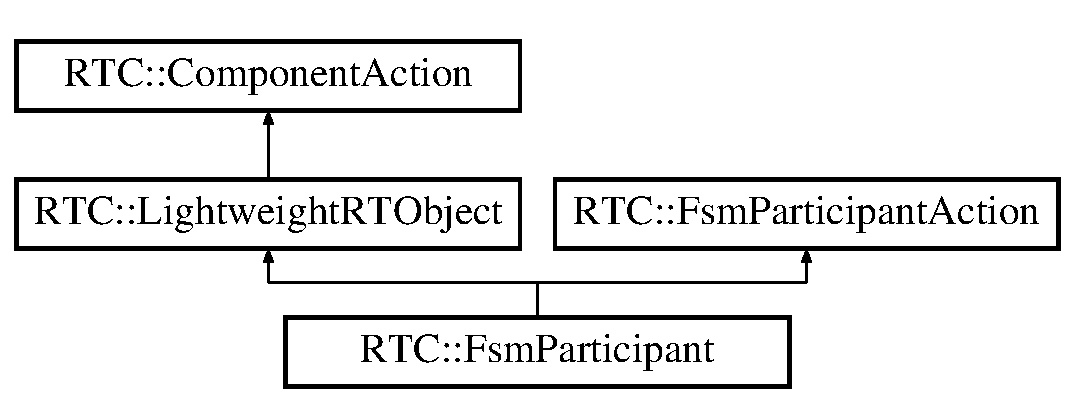
\includegraphics[height=3cm]{interfaceRTC_1_1FsmParticipant}
\end{center}
\end{figure}
\subsection*{Public メソッド}
\begin{DoxyCompactItemize}
\item 
{\bf ReturnCode\_\-t} {\bf initialize} ()
\item 
{\bf ReturnCode\_\-t} {\bf finalize} ()
\item 
boolean {\bf is\_\-alive} (in {\bf ExecutionContext} exec\_\-context)
\item 
{\bf ReturnCode\_\-t} {\bf exit} ()
\item 
{\bf ExecutionContextHandle\_\-t} {\bf attach\_\-context} (in {\bf ExecutionContext} exec\_\-context)
\item 
{\bf ReturnCode\_\-t} {\bf detach\_\-context} (in {\bf ExecutionContextHandle\_\-t} exec\_\-handle)
\item 
{\bf ExecutionContext} {\bf get\_\-context} (in {\bf ExecutionContextHandle\_\-t} exec\_\-handle)
\item 
{\bf ExecutionContextList} {\bf get\_\-owned\_\-contexts} ()
\begin{DoxyCompactList}\small\item\em get\_\-owned\_\-contexts \item\end{DoxyCompactList}\item 
{\bf ExecutionContextList} {\bf get\_\-participating\_\-contexts} ()
\begin{DoxyCompactList}\small\item\em get\_\-participating\_\-contexts \item\end{DoxyCompactList}\item 
{\bf ExecutionContextHandle\_\-t} {\bf get\_\-context\_\-handle} (in {\bf ExecutionContext} cxt)
\item 
{\bf ReturnCode\_\-t} {\bf on\_\-initialize} ()
\item 
{\bf ReturnCode\_\-t} {\bf on\_\-finalize} ()
\item 
{\bf ReturnCode\_\-t} {\bf on\_\-startup} (in {\bf ExecutionContextHandle\_\-t} exec\_\-handle)
\item 
{\bf ReturnCode\_\-t} {\bf on\_\-shutdown} (in {\bf ExecutionContextHandle\_\-t} exec\_\-handle)
\item 
{\bf ReturnCode\_\-t} {\bf on\_\-activated} (in {\bf ExecutionContextHandle\_\-t} exec\_\-handle)
\item 
{\bf ReturnCode\_\-t} {\bf on\_\-deactivated} (in {\bf ExecutionContextHandle\_\-t} exec\_\-handle)
\item 
{\bf ReturnCode\_\-t} {\bf on\_\-aborting} (in {\bf ExecutionContextHandle\_\-t} exec\_\-handle)
\item 
{\bf ReturnCode\_\-t} {\bf on\_\-error} (in {\bf ExecutionContextHandle\_\-t} exec\_\-handle)
\item 
{\bf ReturnCode\_\-t} {\bf on\_\-reset} (in {\bf ExecutionContextHandle\_\-t} exec\_\-handle)
\item 
{\bf ReturnCode\_\-t} {\bf on\_\-action} (in {\bf ExecutionContextHandle\_\-t} exec\_\-handle)
\end{DoxyCompactItemize}


\subsection{関数}
\index{RTC::FsmParticipant@{RTC::FsmParticipant}!attach\_\-context@{attach\_\-context}}
\index{attach\_\-context@{attach\_\-context}!RTC::FsmParticipant@{RTC::FsmParticipant}}
\subsubsection[{attach\_\-context}]{\setlength{\rightskip}{0pt plus 5cm}{\bf ExecutionContextHandle\_\-t} RTC::LightweightRTObject::attach\_\-context (in {\bf ExecutionContext} {\em exec\_\-context})\hspace{0.3cm}{\ttfamily  [inherited]}}\label{interfaceRTC_1_1LightweightRTObject_a48dbdbcac3254c29ad01d43a4ee5a00c}
\index{RTC::FsmParticipant@{RTC::FsmParticipant}!detach\_\-context@{detach\_\-context}}
\index{detach\_\-context@{detach\_\-context}!RTC::FsmParticipant@{RTC::FsmParticipant}}
\subsubsection[{detach\_\-context}]{\setlength{\rightskip}{0pt plus 5cm}{\bf ReturnCode\_\-t} RTC::LightweightRTObject::detach\_\-context (in {\bf ExecutionContextHandle\_\-t} {\em exec\_\-handle})\hspace{0.3cm}{\ttfamily  [inherited]}}\label{interfaceRTC_1_1LightweightRTObject_a8eb94420ca08e8f7acaa778ed883b9a4}
\index{RTC::FsmParticipant@{RTC::FsmParticipant}!exit@{exit}}
\index{exit@{exit}!RTC::FsmParticipant@{RTC::FsmParticipant}}
\subsubsection[{exit}]{\setlength{\rightskip}{0pt plus 5cm}{\bf ReturnCode\_\-t} RTC::LightweightRTObject::exit ()\hspace{0.3cm}{\ttfamily  [inherited]}}\label{interfaceRTC_1_1LightweightRTObject_a49bd940b6964fa80d696db15b45c2f87}
\index{RTC::FsmParticipant@{RTC::FsmParticipant}!finalize@{finalize}}
\index{finalize@{finalize}!RTC::FsmParticipant@{RTC::FsmParticipant}}
\subsubsection[{finalize}]{\setlength{\rightskip}{0pt plus 5cm}{\bf ReturnCode\_\-t} RTC::LightweightRTObject::finalize ()\hspace{0.3cm}{\ttfamily  [inherited]}}\label{interfaceRTC_1_1LightweightRTObject_a23466f177b4289662ea035be831426ad}
\index{RTC::FsmParticipant@{RTC::FsmParticipant}!get\_\-context@{get\_\-context}}
\index{get\_\-context@{get\_\-context}!RTC::FsmParticipant@{RTC::FsmParticipant}}
\subsubsection[{get\_\-context}]{\setlength{\rightskip}{0pt plus 5cm}{\bf ExecutionContext} RTC::LightweightRTObject::get\_\-context (in {\bf ExecutionContextHandle\_\-t} {\em exec\_\-handle})\hspace{0.3cm}{\ttfamily  [inherited]}}\label{interfaceRTC_1_1LightweightRTObject_a7bb123faf81bcb57542c3a17f10948d6}
\index{RTC::FsmParticipant@{RTC::FsmParticipant}!get\_\-context\_\-handle@{get\_\-context\_\-handle}}
\index{get\_\-context\_\-handle@{get\_\-context\_\-handle}!RTC::FsmParticipant@{RTC::FsmParticipant}}
\subsubsection[{get\_\-context\_\-handle}]{\setlength{\rightskip}{0pt plus 5cm}{\bf ExecutionContextHandle\_\-t} RTC::LightweightRTObject::get\_\-context\_\-handle (in {\bf ExecutionContext} {\em cxt})\hspace{0.3cm}{\ttfamily  [inherited]}}\label{interfaceRTC_1_1LightweightRTObject_af54041744c01d68026aa200276e12f45}
\#\#\# [����] \doxyref{RTC.idl}{p.}{RTC_8idl} �ˤϴޤޤ�Ƥ��ʤ���PIM�ˤϴޤޤ�Ƥ��롣 \#\#\# PIM���������� \index{RTC::FsmParticipant@{RTC::FsmParticipant}!get\_\-owned\_\-contexts@{get\_\-owned\_\-contexts}}
\index{get\_\-owned\_\-contexts@{get\_\-owned\_\-contexts}!RTC::FsmParticipant@{RTC::FsmParticipant}}
\subsubsection[{get\_\-owned\_\-contexts}]{\setlength{\rightskip}{0pt plus 5cm}{\bf ExecutionContextList} RTC::LightweightRTObject::get\_\-owned\_\-contexts ()\hspace{0.3cm}{\ttfamily  [inherited]}}\label{interfaceRTC_1_1LightweightRTObject_aea9dd2a447cc3ddc55f20aab698da408}


get\_\-owned\_\-contexts 

\subsection{Description}\label{interfaceRTC_1_1LightweightRTObject_Description}
���� \doxyref{RTC}{p.}{namespaceRTC} ����ͭ���� \doxyref{ExecutionContext}{p.}{interfaceRTC_1_1ExecutionContext} �Υꥹ�Ȥ�������롣 \index{RTC::FsmParticipant@{RTC::FsmParticipant}!get\_\-participating\_\-contexts@{get\_\-participating\_\-contexts}}
\index{get\_\-participating\_\-contexts@{get\_\-participating\_\-contexts}!RTC::FsmParticipant@{RTC::FsmParticipant}}
\subsubsection[{get\_\-participating\_\-contexts}]{\setlength{\rightskip}{0pt plus 5cm}{\bf ExecutionContextList} RTC::LightweightRTObject::get\_\-participating\_\-contexts ()\hspace{0.3cm}{\ttfamily  [inherited]}}\label{interfaceRTC_1_1LightweightRTObject_af2224880b89275ecf82efad0999b022a}


get\_\-participating\_\-contexts 

\subsection{Description}\label{interfaceRTC_1_1LightweightRTObject_Description}
���� \doxyref{RTC}{p.}{namespaceRTC} �����ä��Ƥ��뤹�٤Ƥ� \doxyref{ExecutionContext}{p.}{interfaceRTC_1_1ExecutionContext} �Υꥹ�Ȥ�������롣\subsection{Semantics}\label{interfaceRTC_1_1LightweightRTObject_Semantics}
���Υꥹ�Ȥ˴ޤޤ��¹ԥ���ƥ����Ȥϡ�attach\_\-context ���Ƥӽ� ����뤴�Ȥˡ��ꥹ�Ȥ��ɲä��졢detach\_\-context ���ƤӽФ���뤴 �Ȥˡ��ꥹ�Ȥ���������롣 \index{RTC::FsmParticipant@{RTC::FsmParticipant}!initialize@{initialize}}
\index{initialize@{initialize}!RTC::FsmParticipant@{RTC::FsmParticipant}}
\subsubsection[{initialize}]{\setlength{\rightskip}{0pt plus 5cm}{\bf ReturnCode\_\-t} RTC::LightweightRTObject::initialize ()\hspace{0.3cm}{\ttfamily  [inherited]}}\label{interfaceRTC_1_1LightweightRTObject_afb28c4d97677804da09488578b840eb5}
\index{RTC::FsmParticipant@{RTC::FsmParticipant}!is\_\-alive@{is\_\-alive}}
\index{is\_\-alive@{is\_\-alive}!RTC::FsmParticipant@{RTC::FsmParticipant}}
\subsubsection[{is\_\-alive}]{\setlength{\rightskip}{0pt plus 5cm}boolean RTC::LightweightRTObject::is\_\-alive (in {\bf ExecutionContext} {\em exec\_\-context})\hspace{0.3cm}{\ttfamily  [inherited]}}\label{interfaceRTC_1_1LightweightRTObject_aa07c8c299b0addc49887508c1ee7be27}
\index{RTC::FsmParticipant@{RTC::FsmParticipant}!on\_\-aborting@{on\_\-aborting}}
\index{on\_\-aborting@{on\_\-aborting}!RTC::FsmParticipant@{RTC::FsmParticipant}}
\subsubsection[{on\_\-aborting}]{\setlength{\rightskip}{0pt plus 5cm}{\bf ReturnCode\_\-t} RTC::ComponentAction::on\_\-aborting (in {\bf ExecutionContextHandle\_\-t} {\em exec\_\-handle})\hspace{0.3cm}{\ttfamily  [inherited]}}\label{interfaceRTC_1_1ComponentAction_a876e58ebcea16c307e131b3e6a58ddbe}
\index{RTC::FsmParticipant@{RTC::FsmParticipant}!on\_\-action@{on\_\-action}}
\index{on\_\-action@{on\_\-action}!RTC::FsmParticipant@{RTC::FsmParticipant}}
\subsubsection[{on\_\-action}]{\setlength{\rightskip}{0pt plus 5cm}{\bf ReturnCode\_\-t} RTC::FsmParticipantAction::on\_\-action (in {\bf ExecutionContextHandle\_\-t} {\em exec\_\-handle})\hspace{0.3cm}{\ttfamily  [inherited]}}\label{interfaceRTC_1_1FsmParticipantAction_ae627f5cdc59f586246bb2174797c7864}
\index{RTC::FsmParticipant@{RTC::FsmParticipant}!on\_\-activated@{on\_\-activated}}
\index{on\_\-activated@{on\_\-activated}!RTC::FsmParticipant@{RTC::FsmParticipant}}
\subsubsection[{on\_\-activated}]{\setlength{\rightskip}{0pt plus 5cm}{\bf ReturnCode\_\-t} RTC::ComponentAction::on\_\-activated (in {\bf ExecutionContextHandle\_\-t} {\em exec\_\-handle})\hspace{0.3cm}{\ttfamily  [inherited]}}\label{interfaceRTC_1_1ComponentAction_a4f51f627067d0c54e89c4c0827fa6432}
\index{RTC::FsmParticipant@{RTC::FsmParticipant}!on\_\-deactivated@{on\_\-deactivated}}
\index{on\_\-deactivated@{on\_\-deactivated}!RTC::FsmParticipant@{RTC::FsmParticipant}}
\subsubsection[{on\_\-deactivated}]{\setlength{\rightskip}{0pt plus 5cm}{\bf ReturnCode\_\-t} RTC::ComponentAction::on\_\-deactivated (in {\bf ExecutionContextHandle\_\-t} {\em exec\_\-handle})\hspace{0.3cm}{\ttfamily  [inherited]}}\label{interfaceRTC_1_1ComponentAction_aa5f9cfb9677ba685be333ad666c87f88}
\index{RTC::FsmParticipant@{RTC::FsmParticipant}!on\_\-error@{on\_\-error}}
\index{on\_\-error@{on\_\-error}!RTC::FsmParticipant@{RTC::FsmParticipant}}
\subsubsection[{on\_\-error}]{\setlength{\rightskip}{0pt plus 5cm}{\bf ReturnCode\_\-t} RTC::ComponentAction::on\_\-error (in {\bf ExecutionContextHandle\_\-t} {\em exec\_\-handle})\hspace{0.3cm}{\ttfamily  [inherited]}}\label{interfaceRTC_1_1ComponentAction_a110fdde803e9b13f27308b897439962a}
\index{RTC::FsmParticipant@{RTC::FsmParticipant}!on\_\-finalize@{on\_\-finalize}}
\index{on\_\-finalize@{on\_\-finalize}!RTC::FsmParticipant@{RTC::FsmParticipant}}
\subsubsection[{on\_\-finalize}]{\setlength{\rightskip}{0pt plus 5cm}{\bf ReturnCode\_\-t} RTC::ComponentAction::on\_\-finalize ()\hspace{0.3cm}{\ttfamily  [inherited]}}\label{interfaceRTC_1_1ComponentAction_a9c9e2d638cd2b748609be8a23410aedc}
\index{RTC::FsmParticipant@{RTC::FsmParticipant}!on\_\-initialize@{on\_\-initialize}}
\index{on\_\-initialize@{on\_\-initialize}!RTC::FsmParticipant@{RTC::FsmParticipant}}
\subsubsection[{on\_\-initialize}]{\setlength{\rightskip}{0pt plus 5cm}{\bf ReturnCode\_\-t} RTC::ComponentAction::on\_\-initialize ()\hspace{0.3cm}{\ttfamily  [inherited]}}\label{interfaceRTC_1_1ComponentAction_a8703b183bc1bed9e2fd3ecac126cb231}
\index{RTC::FsmParticipant@{RTC::FsmParticipant}!on\_\-reset@{on\_\-reset}}
\index{on\_\-reset@{on\_\-reset}!RTC::FsmParticipant@{RTC::FsmParticipant}}
\subsubsection[{on\_\-reset}]{\setlength{\rightskip}{0pt plus 5cm}{\bf ReturnCode\_\-t} RTC::ComponentAction::on\_\-reset (in {\bf ExecutionContextHandle\_\-t} {\em exec\_\-handle})\hspace{0.3cm}{\ttfamily  [inherited]}}\label{interfaceRTC_1_1ComponentAction_adb0e61bff251337d79c7c7d050d8304e}
\index{RTC::FsmParticipant@{RTC::FsmParticipant}!on\_\-shutdown@{on\_\-shutdown}}
\index{on\_\-shutdown@{on\_\-shutdown}!RTC::FsmParticipant@{RTC::FsmParticipant}}
\subsubsection[{on\_\-shutdown}]{\setlength{\rightskip}{0pt plus 5cm}{\bf ReturnCode\_\-t} RTC::ComponentAction::on\_\-shutdown (in {\bf ExecutionContextHandle\_\-t} {\em exec\_\-handle})\hspace{0.3cm}{\ttfamily  [inherited]}}\label{interfaceRTC_1_1ComponentAction_accc47711344c811c9bdba0d66a3048f2}
\index{RTC::FsmParticipant@{RTC::FsmParticipant}!on\_\-startup@{on\_\-startup}}
\index{on\_\-startup@{on\_\-startup}!RTC::FsmParticipant@{RTC::FsmParticipant}}
\subsubsection[{on\_\-startup}]{\setlength{\rightskip}{0pt plus 5cm}{\bf ReturnCode\_\-t} RTC::ComponentAction::on\_\-startup (in {\bf ExecutionContextHandle\_\-t} {\em exec\_\-handle})\hspace{0.3cm}{\ttfamily  [inherited]}}\label{interfaceRTC_1_1ComponentAction_ac305f00c92f4650cf4fc798aac37eef2}


このインタフェースの説明は次のファイルから生成されました:\begin{DoxyCompactItemize}
\item 
{\bf RTC.idl}\end{DoxyCompactItemize}

\section{RTC::FsmParticipantAction Interface Reference}
\label{interfaceRTC_1_1FsmParticipantAction}\index{RTC::FsmParticipantAction@{RTC::FsmParticipantAction}}


\doxyref{FsmParticipantAction}{p.}{interfaceRTC_1_1FsmParticipantAction}.  




{\ttfamily import \char`\"{}RTC.idl\char`\"{};}

Inheritance diagram for RTC::FsmParticipantAction:\begin{figure}[H]
\begin{center}
\leavevmode
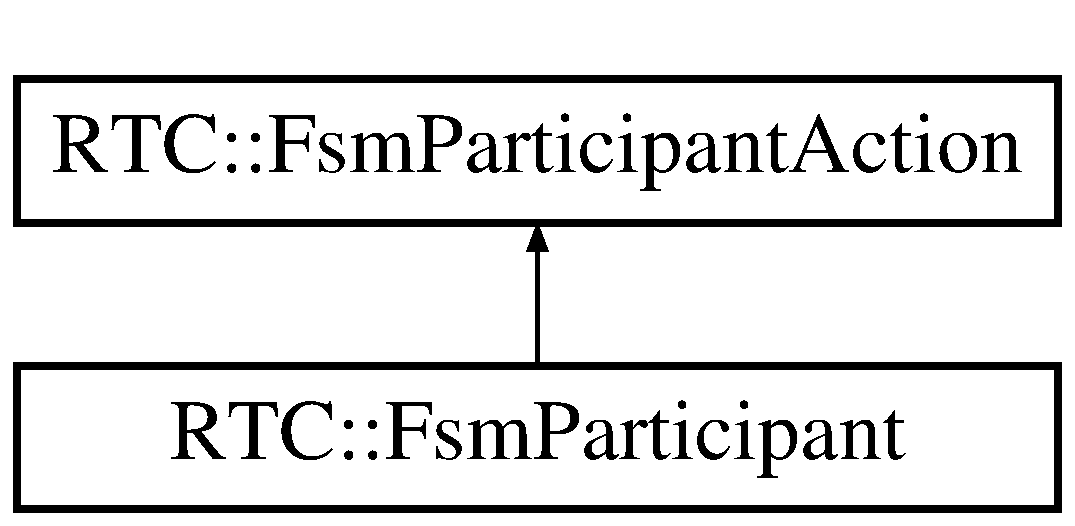
\includegraphics[height=2cm]{interfaceRTC_1_1FsmParticipantAction}
\end{center}
\end{figure}
\subsection*{Public Member Functions}
\begin{DoxyCompactItemize}
\item 
{\bf ReturnCode\_\-t} {\bf on\_\-action} (in {\bf ExecutionContextHandle\_\-t} exec\_\-handle)
\begin{DoxyCompactList}\small\item\em on\_\-action \item\end{DoxyCompactList}\end{DoxyCompactItemize}


\subsection{Detailed Description}
\doxyref{FsmParticipantAction}{p.}{interfaceRTC_1_1FsmParticipantAction}. \subsection{Description}\label{namespaceRTC_Description}
\doxyref{FsmParticipantAction}{p.}{interfaceRTC_1_1FsmParticipantAction} is companion to \doxyref{ComponentAction}{p.}{interfaceRTC_1_1ComponentAction} (see Section 5.2.2.4) that is intended for use with FSM participant RTCs. It adds a callback for the interception of state transitions, state entries, and state exits. 

\subsection{Member Function Documentation}
\index{RTC::FsmParticipantAction@{RTC::FsmParticipantAction}!on\_\-action@{on\_\-action}}
\index{on\_\-action@{on\_\-action}!RTC::FsmParticipantAction@{RTC::FsmParticipantAction}}
\subsubsection[{on\_\-action}]{\setlength{\rightskip}{0pt plus 5cm}{\bf ReturnCode\_\-t} RTC::FsmParticipantAction::on\_\-action (in {\bf ExecutionContextHandle\_\-t} {\em exec\_\-handle})}\label{interfaceRTC_1_1FsmParticipantAction_ae627f5cdc59f586246bb2174797c7864}


on\_\-action 

\subsection{Description}\label{namespaceRTC_Description}
The indicated FSM participant \doxyref{RTC}{p.}{namespaceRTC} has been invoked as a result of a transition, state entry, or state exit in its containing FSM.\subsection{Constraints}\label{interfaceRTC_1_1LightweightRTObject_Constraints}

\begin{DoxyItemize}
\item The given execution context shall be of kind EVENT\_\-DRIVEN. 
\end{DoxyItemize}

The documentation for this interface was generated from the following file:\begin{DoxyCompactItemize}
\item 
{\bf RTC.idl}\end{DoxyCompactItemize}

\section{RTC::FsmProfile Struct Reference}
\label{structRTC_1_1FsmProfile}\index{RTC::FsmProfile@{RTC::FsmProfile}}


\doxyref{FsmProfile}{p.}{structRTC_1_1FsmProfile}.  




{\ttfamily import \char`\"{}RTC.idl\char`\"{};}

\subsection*{Public Attributes}
\begin{DoxyCompactItemize}
\item 
{\bf FsmBehaviorProfileList} {\bf behavior\_\-profiles}
\begin{DoxyCompactList}\small\item\em behavior\_\-profiles \item\end{DoxyCompactList}\end{DoxyCompactItemize}


\subsection{Detailed Description}
\doxyref{FsmProfile}{p.}{structRTC_1_1FsmProfile}. \subsection{Description}\label{namespaceRTC_Description}
The \doxyref{FsmProfile}{p.}{structRTC_1_1FsmProfile} describes the correspondence between an FSM and its contained FSM participants. This Profile is necessary for Stimulus Response Processing. 

\subsection{Member Data Documentation}
\index{RTC::FsmProfile@{RTC::FsmProfile}!behavior\_\-profiles@{behavior\_\-profiles}}
\index{behavior\_\-profiles@{behavior\_\-profiles}!RTC::FsmProfile@{RTC::FsmProfile}}
\subsubsection[{behavior\_\-profiles}]{\setlength{\rightskip}{0pt plus 5cm}{\bf FsmBehaviorProfileList} {\bf RTC::FsmProfile::behavior\_\-profiles}}\label{structRTC_1_1FsmProfile_a3f1aa3d58fcd0beb4ed3ac833487856d}


behavior\_\-profiles 

\subsection{Description}\label{namespaceRTC_Description}
This attribute lists the correspondences between an FSM and its contained FSM participants. 

The documentation for this struct was generated from the following file:\begin{DoxyCompactItemize}
\item 
{\bf RTC.idl}\end{DoxyCompactItemize}

\section{インタフェース RTC::FsmService}
\label{interfaceRTC_1_1FsmService}\index{RTC::FsmService@{RTC::FsmService}}


{\ttfamily import \char`\"{}RTC.idl\char`\"{};}

RTC::FsmServiceに対する継承グラフ\begin{figure}[H]
\begin{center}
\leavevmode
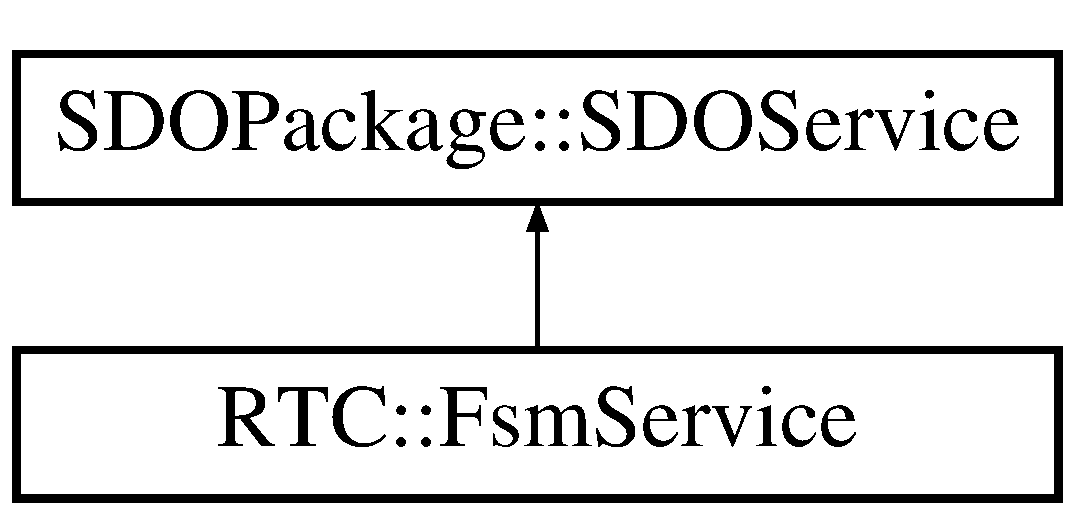
\includegraphics[height=2cm]{interfaceRTC_1_1FsmService}
\end{center}
\end{figure}
\subsection*{Public メソッド}
\begin{DoxyCompactItemize}
\item 
{\bf FsmProfile} {\bf get\_\-fsm\_\-profile} ()
\item 
{\bf ReturnCode\_\-t} {\bf set\_\-fsm\_\-profile} (in {\bf FsmProfile} fsm\_\-profile)
\end{DoxyCompactItemize}


\subsection{関数}
\index{RTC::FsmService@{RTC::FsmService}!get\_\-fsm\_\-profile@{get\_\-fsm\_\-profile}}
\index{get\_\-fsm\_\-profile@{get\_\-fsm\_\-profile}!RTC::FsmService@{RTC::FsmService}}
\subsubsection[{get\_\-fsm\_\-profile}]{\setlength{\rightskip}{0pt plus 5cm}{\bf FsmProfile} RTC::FsmService::get\_\-fsm\_\-profile ()}\label{interfaceRTC_1_1FsmService_a72907dcf0995ba5e06b9867d2954944a}
\index{RTC::FsmService@{RTC::FsmService}!set\_\-fsm\_\-profile@{set\_\-fsm\_\-profile}}
\index{set\_\-fsm\_\-profile@{set\_\-fsm\_\-profile}!RTC::FsmService@{RTC::FsmService}}
\subsubsection[{set\_\-fsm\_\-profile}]{\setlength{\rightskip}{0pt plus 5cm}{\bf ReturnCode\_\-t} RTC::FsmService::set\_\-fsm\_\-profile (in {\bf FsmProfile} {\em fsm\_\-profile})}\label{interfaceRTC_1_1FsmService_a492ee38ee1914d430c2f456861e2471f}


このインタフェースの説明は次のファイルから生成されました:\begin{DoxyCompactItemize}
\item 
{\bf RTC.idl}\end{DoxyCompactItemize}

\section{インタフェース OpenRTM::InPortCdr}
\label{interfaceOpenRTM_1_1InPortCdr}\index{OpenRTM::InPortCdr@{OpenRTM::InPortCdr}}


{\ttfamily import \char`\"{}DataPort.idl\char`\"{};}

\subsection*{Public メソッド}
\begin{DoxyCompactItemize}
\item 
{\bf PortStatus} {\bf put} (in {\bf CdrData} data)
\end{DoxyCompactItemize}


\subsection{関数}
\index{OpenRTM::InPortCdr@{OpenRTM::InPortCdr}!put@{put}}
\index{put@{put}!OpenRTM::InPortCdr@{OpenRTM::InPortCdr}}
\subsubsection[{put}]{\setlength{\rightskip}{0pt plus 5cm}{\bf PortStatus} OpenRTM::InPortCdr::put (in {\bf CdrData} {\em data})}\label{interfaceOpenRTM_1_1InPortCdr_a25c06cc0054c091c33dbe23398cc11c4}


このインタフェースの説明は次のファイルから生成されました:\begin{DoxyCompactItemize}
\item 
{\bf DataPort.idl}\end{DoxyCompactItemize}

\section{SDOPackage::IntervalType Struct Reference}
\label{structSDOPackage_1_1IntervalType}\index{SDOPackage::IntervalType@{SDOPackage::IntervalType}}


{\ttfamily import \char`\"{}SDOPackage.idl\char`\"{};}

\subsection*{Public Attributes}
\begin{DoxyCompactItemize}
\item 
{\bf Numeric} {\bf min}
\item 
{\bf Numeric} {\bf max}
\item 
boolean {\bf min\_\-inclusive}
\item 
boolean {\bf max\_\-inclusive}
\item 
{\bf Numeric} {\bf step}
\end{DoxyCompactItemize}


\subsection{Member Data Documentation}
\index{SDOPackage::IntervalType@{SDOPackage::IntervalType}!max@{max}}
\index{max@{max}!SDOPackage::IntervalType@{SDOPackage::IntervalType}}
\subsubsection[{max}]{\setlength{\rightskip}{0pt plus 5cm}{\bf Numeric} {\bf SDOPackage::IntervalType::max}}\label{structSDOPackage_1_1IntervalType_aa712935cd3564a4ccef14713b278d1b1}
\index{SDOPackage::IntervalType@{SDOPackage::IntervalType}!max\_\-inclusive@{max\_\-inclusive}}
\index{max\_\-inclusive@{max\_\-inclusive}!SDOPackage::IntervalType@{SDOPackage::IntervalType}}
\subsubsection[{max\_\-inclusive}]{\setlength{\rightskip}{0pt plus 5cm}boolean {\bf SDOPackage::IntervalType::max\_\-inclusive}}\label{structSDOPackage_1_1IntervalType_ab91d204fe571aa33a74631745aaf6e29}
\index{SDOPackage::IntervalType@{SDOPackage::IntervalType}!min@{min}}
\index{min@{min}!SDOPackage::IntervalType@{SDOPackage::IntervalType}}
\subsubsection[{min}]{\setlength{\rightskip}{0pt plus 5cm}{\bf Numeric} {\bf SDOPackage::IntervalType::min}}\label{structSDOPackage_1_1IntervalType_a3f0d49fb52fe8f19143921c44bd3990f}
\index{SDOPackage::IntervalType@{SDOPackage::IntervalType}!min\_\-inclusive@{min\_\-inclusive}}
\index{min\_\-inclusive@{min\_\-inclusive}!SDOPackage::IntervalType@{SDOPackage::IntervalType}}
\subsubsection[{min\_\-inclusive}]{\setlength{\rightskip}{0pt plus 5cm}boolean {\bf SDOPackage::IntervalType::min\_\-inclusive}}\label{structSDOPackage_1_1IntervalType_a1c39de81fb0c54339e906701a0874ef0}
\index{SDOPackage::IntervalType@{SDOPackage::IntervalType}!step@{step}}
\index{step@{step}!SDOPackage::IntervalType@{SDOPackage::IntervalType}}
\subsubsection[{step}]{\setlength{\rightskip}{0pt plus 5cm}{\bf Numeric} {\bf SDOPackage::IntervalType::step}}\label{structSDOPackage_1_1IntervalType_a8adfa6cc83bff1b0998457429290958f}


The documentation for this struct was generated from the following file:\begin{DoxyCompactItemize}
\item 
{\bf SDOPackage.idl}\end{DoxyCompactItemize}

\section{RTC::LightweightRTObject Interface Reference}
\label{interfaceRTC_1_1LightweightRTObject}\index{RTC::LightweightRTObject@{RTC::LightweightRTObject}}


\doxyref{LightweightRTObject}{p.}{interfaceRTC_1_1LightweightRTObject}.  




{\ttfamily import \char`\"{}RTC.idl\char`\"{};}

Inheritance diagram for RTC::LightweightRTObject:\begin{figure}[H]
\begin{center}
\leavevmode
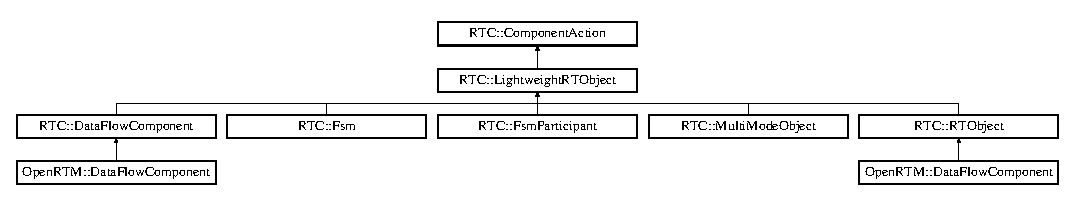
\includegraphics[height=2.25126cm]{interfaceRTC_1_1LightweightRTObject}
\end{center}
\end{figure}
\subsection*{Public Member Functions}
\begin{DoxyCompactItemize}
\item 
{\bf ReturnCode\_\-t} {\bf initialize} ()
\begin{DoxyCompactList}\small\item\em initialize \item\end{DoxyCompactList}\item 
{\bf ReturnCode\_\-t} {\bf finalize} ()
\begin{DoxyCompactList}\small\item\em finalize \item\end{DoxyCompactList}\item 
boolean {\bf is\_\-alive} (in {\bf ExecutionContext} exec\_\-context)
\begin{DoxyCompactList}\small\item\em is\_\-alive \item\end{DoxyCompactList}\item 
{\bf ReturnCode\_\-t} {\bf exit} ()
\begin{DoxyCompactList}\small\item\em exit \item\end{DoxyCompactList}\item 
{\bf ExecutionContextHandle\_\-t} {\bf attach\_\-context} (in {\bf ExecutionContext} exec\_\-context)
\begin{DoxyCompactList}\small\item\em attach\_\-context \item\end{DoxyCompactList}\item 
{\bf ReturnCode\_\-t} {\bf detach\_\-context} (in {\bf ExecutionContextHandle\_\-t} exec\_\-handle)
\begin{DoxyCompactList}\small\item\em detach\_\-context \item\end{DoxyCompactList}\item 
{\bf ExecutionContext} {\bf get\_\-context} (in {\bf ExecutionContextHandle\_\-t} exec\_\-handle)
\begin{DoxyCompactList}\small\item\em get\_\-context \item\end{DoxyCompactList}\item 
{\bf ExecutionContextList} {\bf get\_\-owned\_\-contexts} ()
\begin{DoxyCompactList}\small\item\em get\_\-owned\_\-contexts \item\end{DoxyCompactList}\item 
{\bf ExecutionContextList} {\bf get\_\-participating\_\-contexts} ()
\begin{DoxyCompactList}\small\item\em $\ast$ get\_\-participating\_\-contexts \item\end{DoxyCompactList}\item 
{\bf ExecutionContextHandle\_\-t} {\bf get\_\-context\_\-handle} (in {\bf ExecutionContext} cxt)
\begin{DoxyCompactList}\small\item\em get\_\-context\_\-handle \item\end{DoxyCompactList}\item 
{\bf ReturnCode\_\-t} {\bf on\_\-initialize} ()
\begin{DoxyCompactList}\small\item\em on\_\-initialize \item\end{DoxyCompactList}\item 
{\bf ReturnCode\_\-t} {\bf on\_\-finalize} ()
\begin{DoxyCompactList}\small\item\em on\_\-finalize \item\end{DoxyCompactList}\item 
{\bf ReturnCode\_\-t} {\bf on\_\-startup} (in {\bf ExecutionContextHandle\_\-t} exec\_\-handle)
\begin{DoxyCompactList}\small\item\em on\_\-startup \item\end{DoxyCompactList}\item 
{\bf ReturnCode\_\-t} {\bf on\_\-shutdown} (in {\bf ExecutionContextHandle\_\-t} exec\_\-handle)
\begin{DoxyCompactList}\small\item\em on\_\-shutdown \item\end{DoxyCompactList}\item 
{\bf ReturnCode\_\-t} {\bf on\_\-activated} (in {\bf ExecutionContextHandle\_\-t} exec\_\-handle)
\begin{DoxyCompactList}\small\item\em on\_\-activated \item\end{DoxyCompactList}\item 
{\bf ReturnCode\_\-t} {\bf on\_\-deactivated} (in {\bf ExecutionContextHandle\_\-t} exec\_\-handle)
\begin{DoxyCompactList}\small\item\em on\_\-deactivated \item\end{DoxyCompactList}\item 
{\bf ReturnCode\_\-t} {\bf on\_\-aborting} (in {\bf ExecutionContextHandle\_\-t} exec\_\-handle)
\begin{DoxyCompactList}\small\item\em on\_\-aborting \item\end{DoxyCompactList}\item 
{\bf ReturnCode\_\-t} {\bf on\_\-error} (in {\bf ExecutionContextHandle\_\-t} exec\_\-handle)
\begin{DoxyCompactList}\small\item\em on\_\-error \item\end{DoxyCompactList}\item 
{\bf ReturnCode\_\-t} {\bf on\_\-reset} (in {\bf ExecutionContextHandle\_\-t} exec\_\-handle)
\begin{DoxyCompactList}\small\item\em on\_\-reset \item\end{DoxyCompactList}\end{DoxyCompactItemize}


\subsection{Detailed Description}
\doxyref{LightweightRTObject}{p.}{interfaceRTC_1_1LightweightRTObject}. \subsection{Description}\label{namespaceRTC_Description}
This interface is realized by all lightweight RTCs (as required by the lightweightRTComponent stereotype). It defines the states and transitions through which all RTCs will pass from the time they are created until the time they are destroyed.\subsection{Semantics}\label{namespaceRTC_Semantics}
\subsubsection{Initialization}\label{interfaceRTC_1_1LightweightRTObject_Initialization}
An \doxyref{RTC}{p.}{namespaceRTC} begins in the Created state; at this point, it has been instantiated but not yet fully initialized. Note that this state is highly implementation-\/dependent. For example, it may correspond to the invocation of a constructor in languages that support that concept, but not all languages do. Furthermore, how soon this state is entered before initialize is invoked is implementation-\/dependent. Therefore, it should be relied on by \doxyref{RTC}{p.}{namespaceRTC} implementers only to the minimum extent possible. An \doxyref{RTC}{p.}{namespaceRTC} that has completed its initialization and has not been finalized is said to be Alive.\subsubsection{Context}\label{interfaceRTC_1_1LightweightRTObject_Execution}
An \doxyref{RTC}{p.}{namespaceRTC} in the Alive state may participate in any number of execution contexts (see Section 5.2.2.5 ). These contexts shall be represented to an \doxyref{RTC}{p.}{namespaceRTC} as distinct instances of the \doxyref{ExecutionContext}{p.}{interfaceRTC_1_1ExecutionContext} class. The \doxyref{ExecutionContext}{p.}{interfaceRTC_1_1ExecutionContext} manages the behavior of each \doxyref{RTC}{p.}{namespaceRTC} that participates in it. This relationship is defined by the following state machine, which is embedded within the ExecutionContext's own lifecycle (see Figure 5.5 ). Each participating \doxyref{RTC}{p.}{namespaceRTC} is represented as a separate parallel region.

Relative to a given execution context, an \doxyref{RTC}{p.}{namespaceRTC} may either be Active, Inactive, or in Error. When the \doxyref{RTC}{p.}{namespaceRTC} is Active in a Running execution context, the \doxyref{ComponentAction}{p.}{interfaceRTC_1_1ComponentAction} callbacks (see Section 5.2.2.4) shall be invoked as appropriate for the context�� s ExecutionKind. The callbacks shall not be invoked relative to that context when either the \doxyref{RTC}{p.}{namespaceRTC} is Inactive in that context or the context is Stopped. (Note that starting and stopping an execution context shall not impact whether its participating RTCs are Active or Inactive.) It may be that a given \doxyref{RTC}{p.}{namespaceRTC} does not directly participate in any execution contexts. Such an \doxyref{RTC}{p.}{namespaceRTC} is referred to as passive. A passive \doxyref{RTC}{p.}{namespaceRTC} may provide services to other components upon request. At any other time, it shall not be required to perform any ongoing activity of its own; therefore, instances of such an \doxyref{RTC}{p.}{namespaceRTC} typically exist only as parts (directly or indirectly) of a containing active \doxyref{RTC}{p.}{namespaceRTC}.\subsubsection{Handling}\label{interfaceRTC_1_1LightweightRTObject_Error}
If an operation fails while the \doxyref{RTC}{p.}{namespaceRTC} is Active in a given execution context, the \doxyref{RTC}{p.}{namespaceRTC} will transition to the Error state corresponding to that context. While the \doxyref{RTC}{p.}{namespaceRTC} is in Error, the \doxyref{ComponentAction::on\_\-error}{p.}{interfaceRTC_1_1ComponentAction_a110fdde803e9b13f27308b897439962a} callback will be invoked in place of those callbacks that would otherwise have been invoked according to the context��s ExecutionKind. For example, if the kind is PERIODIC, on\_\-error shall be invoked instead of the pair of on\_\-execute, and on\_\-state\_\-update. When an \doxyref{RTC}{p.}{namespaceRTC} is in Error, it may be reset. If resetting is successful, the \doxyref{RTC}{p.}{namespaceRTC} shall return to the Inactive state. If resetting is unsuccessful, it shall remain in the Error state. 

\subsection{Member Function Documentation}
\index{RTC::LightweightRTObject@{RTC::LightweightRTObject}!attach\_\-context@{attach\_\-context}}
\index{attach\_\-context@{attach\_\-context}!RTC::LightweightRTObject@{RTC::LightweightRTObject}}
\subsubsection[{attach\_\-context}]{\setlength{\rightskip}{0pt plus 5cm}{\bf ExecutionContextHandle\_\-t} RTC::LightweightRTObject::attach\_\-context (in {\bf ExecutionContext} {\em exec\_\-context})}\label{interfaceRTC_1_1LightweightRTObject_a48dbdbcac3254c29ad01d43a4ee5a00c}


attach\_\-context 

\subsection{Description}\label{namespaceRTC_Description}
Inform this \doxyref{RTC}{p.}{namespaceRTC} that it is participating in the given execution context. Return a handle that represents the association of this \doxyref{RTC}{p.}{namespaceRTC} with the context.\subsection{Semantics}\label{namespaceRTC_Semantics}
This operation is intended to be invoked by ExecutionContextOperations::add\_\-component (see Section 5.2.2.6.6). It is not intended for use by other clients. \index{RTC::LightweightRTObject@{RTC::LightweightRTObject}!detach\_\-context@{detach\_\-context}}
\index{detach\_\-context@{detach\_\-context}!RTC::LightweightRTObject@{RTC::LightweightRTObject}}
\subsubsection[{detach\_\-context}]{\setlength{\rightskip}{0pt plus 5cm}{\bf ReturnCode\_\-t} RTC::LightweightRTObject::detach\_\-context (in {\bf ExecutionContextHandle\_\-t} {\em exec\_\-handle})}\label{interfaceRTC_1_1LightweightRTObject_a8eb94420ca08e8f7acaa778ed883b9a4}


detach\_\-context 

\subsection{Description}\label{namespaceRTC_Description}
Inform this \doxyref{RTC}{p.}{namespaceRTC} that it is no longer participating in the given execution context.\subsection{Semantics}\label{namespaceRTC_Semantics}
This operation is intended to be invoked by ExecutionContextOperations::remove\_\-component (see Section 5.2.2.6.7). It is not intended for use by other clients.\subsection{Constraints}\label{interfaceRTC_1_1LightweightRTObject_Constraints}

\begin{DoxyItemize}
\item This operation may not be invoked if this \doxyref{RTC}{p.}{namespaceRTC} is not already participating in the execution context. Such a call shall fail with ReturnCode\_\-t::PRECONDITION\_\-NOT\_\-MET.
\end{DoxyItemize}


\begin{DoxyItemize}
\item This operation may not be invoked if this \doxyref{RTC}{p.}{namespaceRTC} is Active in the indicated execution context. Otherwise, it shall fail with ReturnCode\_\-t::PRECONDITION\_\-NOT\_\-MET. 
\end{DoxyItemize}\index{RTC::LightweightRTObject@{RTC::LightweightRTObject}!exit@{exit}}
\index{exit@{exit}!RTC::LightweightRTObject@{RTC::LightweightRTObject}}
\subsubsection[{exit}]{\setlength{\rightskip}{0pt plus 5cm}{\bf ReturnCode\_\-t} RTC::LightweightRTObject::exit ()}\label{interfaceRTC_1_1LightweightRTObject_a49bd940b6964fa80d696db15b45c2f87}


exit 

\subsection{Description}\label{namespaceRTC_Description}
Stop the RTC��s execution context(s) and finalize it along with its contents.\subsection{Semantics}\label{namespaceRTC_Semantics}
Any execution contexts for which the \doxyref{RTC}{p.}{namespaceRTC} is the owner shall be stopped. If the \doxyref{RTC}{p.}{namespaceRTC} participates in any execution contexts belonging to another \doxyref{RTC}{p.}{namespaceRTC} that contains it, directly or indirectly (i.e., the containing \doxyref{RTC}{p.}{namespaceRTC} is the owner of the \doxyref{ExecutionContext}{p.}{interfaceRTC_1_1ExecutionContext}), it shall be deactivated in those contexts. After the \doxyref{RTC}{p.}{namespaceRTC} is no longer Active in any Running execution context, it and any RTCs contained transitively within it shall be finalized.\subsection{Constraints}\label{interfaceRTC_1_1LightweightRTObject_Constraints}
An \doxyref{RTC}{p.}{namespaceRTC} cannot be exited if it has not yet been initialized. Any attempt to exit an \doxyref{RTC}{p.}{namespaceRTC} that is in the Created state shall fail with ReturnCode\_\-t::PRECONDITION\_\-NOT\_\-MET. \index{RTC::LightweightRTObject@{RTC::LightweightRTObject}!finalize@{finalize}}
\index{finalize@{finalize}!RTC::LightweightRTObject@{RTC::LightweightRTObject}}
\subsubsection[{finalize}]{\setlength{\rightskip}{0pt plus 5cm}{\bf ReturnCode\_\-t} RTC::LightweightRTObject::finalize ()}\label{interfaceRTC_1_1LightweightRTObject_a23466f177b4289662ea035be831426ad}


finalize 

\subsection{Description}\label{namespaceRTC_Description}
Finalize the \doxyref{RTC}{p.}{namespaceRTC} that realizes this interface, preparing it for destruction.\subsection{Semantics}\label{namespaceRTC_Semantics}
This invocation of this operation shall result in the invocation of the callback \doxyref{ComponentAction::on\_\-finalize}{p.}{interfaceRTC_1_1ComponentAction_a9c9e2d638cd2b748609be8a23410aedc}\subsection{Constraints}\label{interfaceRTC_1_1LightweightRTObject_Constraints}

\begin{DoxyItemize}
\item An \doxyref{RTC}{p.}{namespaceRTC} may not be finalized while it is participating in any execution context. It must first be removed with ExecutionContextOperations::remove\_\-component. Otherwise, this operation shall fail with ReturnCode\_\-t::PRECONDITION\_\-NOT\_\-MET. See Figure 5.9.
\end{DoxyItemize}


\begin{DoxyItemize}
\item An \doxyref{RTC}{p.}{namespaceRTC} may not be finalized while it is in the Created state. Any attempt to invoke this operation while in that state shall fail with ReturnCode\_\-t::PRECONDITION\_\-NOT\_\-MET.
\end{DoxyItemize}


\begin{DoxyItemize}
\item Application developers are not expected to call this operation directly; it exists for use by the \doxyref{RTC}{p.}{namespaceRTC} infrastructure. 
\end{DoxyItemize}\index{RTC::LightweightRTObject@{RTC::LightweightRTObject}!get\_\-context@{get\_\-context}}
\index{get\_\-context@{get\_\-context}!RTC::LightweightRTObject@{RTC::LightweightRTObject}}
\subsubsection[{get\_\-context}]{\setlength{\rightskip}{0pt plus 5cm}{\bf ExecutionContext} RTC::LightweightRTObject::get\_\-context (in {\bf ExecutionContextHandle\_\-t} {\em exec\_\-handle})}\label{interfaceRTC_1_1LightweightRTObject_a7bb123faf81bcb57542c3a17f10948d6}


get\_\-context 

\subsection{Description}\label{namespaceRTC_Description}
Obtain a reference to the execution context represented by the given handle.\subsection{Semantics}\label{namespaceRTC_Semantics}
The mapping from handle to context is specific to a particular \doxyref{RTC}{p.}{namespaceRTC} instance. The given handle must have been obtained by a previous call to attach\_\-context on this \doxyref{RTC}{p.}{namespaceRTC}. \index{RTC::LightweightRTObject@{RTC::LightweightRTObject}!get\_\-context\_\-handle@{get\_\-context\_\-handle}}
\index{get\_\-context\_\-handle@{get\_\-context\_\-handle}!RTC::LightweightRTObject@{RTC::LightweightRTObject}}
\subsubsection[{get\_\-context\_\-handle}]{\setlength{\rightskip}{0pt plus 5cm}{\bf ExecutionContextHandle\_\-t} RTC::LightweightRTObject::get\_\-context\_\-handle (in {\bf ExecutionContext} {\em cxt})}\label{interfaceRTC_1_1LightweightRTObject_af54041744c01d68026aa200276e12f45}


get\_\-context\_\-handle 

\subsection{Description}\label{namespaceRTC_Description}
This operation returns a handle that is associated with the given execution context. \index{RTC::LightweightRTObject@{RTC::LightweightRTObject}!get\_\-owned\_\-contexts@{get\_\-owned\_\-contexts}}
\index{get\_\-owned\_\-contexts@{get\_\-owned\_\-contexts}!RTC::LightweightRTObject@{RTC::LightweightRTObject}}
\subsubsection[{get\_\-owned\_\-contexts}]{\setlength{\rightskip}{0pt plus 5cm}{\bf ExecutionContextList} RTC::LightweightRTObject::get\_\-owned\_\-contexts ()}\label{interfaceRTC_1_1LightweightRTObject_aea9dd2a447cc3ddc55f20aab698da408}


get\_\-owned\_\-contexts 

\subsection{Description}\label{namespaceRTC_Description}
This operation returns a list of all execution contexts owned by this \doxyref{RTC}{p.}{namespaceRTC}. \index{RTC::LightweightRTObject@{RTC::LightweightRTObject}!get\_\-participating\_\-contexts@{get\_\-participating\_\-contexts}}
\index{get\_\-participating\_\-contexts@{get\_\-participating\_\-contexts}!RTC::LightweightRTObject@{RTC::LightweightRTObject}}
\subsubsection[{get\_\-participating\_\-contexts}]{\setlength{\rightskip}{0pt plus 5cm}{\bf ExecutionContextList} RTC::LightweightRTObject::get\_\-participating\_\-contexts ()}\label{interfaceRTC_1_1LightweightRTObject_af2224880b89275ecf82efad0999b022a}


$\ast$ get\_\-participating\_\-contexts 

\subsection{Description}\label{namespaceRTC_Description}
This operation returns a list of all execution contexts in which this \doxyref{RTC}{p.}{namespaceRTC} participates.\subsection{Semantics}\label{namespaceRTC_Semantics}
Each call to attach\_\-context causes the provided context to be added to this list. Each call to detach\_\-context causes the provided context to be removed from this list. \index{RTC::LightweightRTObject@{RTC::LightweightRTObject}!initialize@{initialize}}
\index{initialize@{initialize}!RTC::LightweightRTObject@{RTC::LightweightRTObject}}
\subsubsection[{initialize}]{\setlength{\rightskip}{0pt plus 5cm}{\bf ReturnCode\_\-t} RTC::LightweightRTObject::initialize ()}\label{interfaceRTC_1_1LightweightRTObject_afb28c4d97677804da09488578b840eb5}


initialize 

\subsection{Description}\label{namespaceRTC_Description}
Initialize the \doxyref{RTC}{p.}{namespaceRTC} that realizes this interface.\subsection{Semantics}\label{namespaceRTC_Semantics}
The invocation of this operation shall result in the invocation of the callback \doxyref{ComponentAction::on\_\-initialize}{p.}{interfaceRTC_1_1ComponentAction_a8703b183bc1bed9e2fd3ecac126cb231}.\subsection{Constraints}\label{interfaceRTC_1_1LightweightRTObject_Constraints}

\begin{DoxyItemize}
\item An \doxyref{RTC}{p.}{namespaceRTC} may be initialized only while it is in the Created state. Any attempt to invoke this operation while in another state shall fail with ReturnCode\_\-t::PRECONDITION\_\-NOT\_\-MET.
\item Application developers are not expected to call this operation directly; it exists for use by the \doxyref{RTC}{p.}{namespaceRTC} infrastructure. 
\end{DoxyItemize}\index{RTC::LightweightRTObject@{RTC::LightweightRTObject}!is\_\-alive@{is\_\-alive}}
\index{is\_\-alive@{is\_\-alive}!RTC::LightweightRTObject@{RTC::LightweightRTObject}}
\subsubsection[{is\_\-alive}]{\setlength{\rightskip}{0pt plus 5cm}boolean RTC::LightweightRTObject::is\_\-alive (in {\bf ExecutionContext} {\em exec\_\-context})}\label{interfaceRTC_1_1LightweightRTObject_aa07c8c299b0addc49887508c1ee7be27}


is\_\-alive 

\subsection{Description}\label{namespaceRTC_Description}
A component is alive or not regardless of the execution context from which it is observed. However, whether or not it is Active, Inactive, or in Error is dependent on the execution context(s) (see Figure 5.7) in which it is running. That is, it may be Active in one context but Inactive in another. Therefore, this operation shall report whether this \doxyref{RTC}{p.}{namespaceRTC} is either Active, Inactive, or in Error; which of those states a component is in with respect to a particular context may be queried from the context itself. \index{RTC::LightweightRTObject@{RTC::LightweightRTObject}!on\_\-aborting@{on\_\-aborting}}
\index{on\_\-aborting@{on\_\-aborting}!RTC::LightweightRTObject@{RTC::LightweightRTObject}}
\subsubsection[{on\_\-aborting}]{\setlength{\rightskip}{0pt plus 5cm}{\bf ReturnCode\_\-t} RTC::ComponentAction::on\_\-aborting (in {\bf ExecutionContextHandle\_\-t} {\em exec\_\-handle})\hspace{0.3cm}{\ttfamily  [inherited]}}\label{interfaceRTC_1_1ComponentAction_a876e58ebcea16c307e131b3e6a58ddbe}


on\_\-aborting 

\subsection{Description}\label{namespaceRTC_Description}
The \doxyref{RTC}{p.}{namespaceRTC} is transitioning from the Active state to the Error state in some execution context.\subsection{Semantics}\label{namespaceRTC_Semantics}
This callback is invoked only a single time for time that the \doxyref{RTC}{p.}{namespaceRTC} transitions into the Error state from another state. This behavior is in contrast to that of on\_\-error. \index{RTC::LightweightRTObject@{RTC::LightweightRTObject}!on\_\-activated@{on\_\-activated}}
\index{on\_\-activated@{on\_\-activated}!RTC::LightweightRTObject@{RTC::LightweightRTObject}}
\subsubsection[{on\_\-activated}]{\setlength{\rightskip}{0pt plus 5cm}{\bf ReturnCode\_\-t} RTC::ComponentAction::on\_\-activated (in {\bf ExecutionContextHandle\_\-t} {\em exec\_\-handle})\hspace{0.3cm}{\ttfamily  [inherited]}}\label{interfaceRTC_1_1ComponentAction_a4f51f627067d0c54e89c4c0827fa6432}


on\_\-activated 

\subsection{Description}\label{namespaceRTC_Description}
The \doxyref{RTC}{p.}{namespaceRTC} has been activated in the given execution context. \index{RTC::LightweightRTObject@{RTC::LightweightRTObject}!on\_\-deactivated@{on\_\-deactivated}}
\index{on\_\-deactivated@{on\_\-deactivated}!RTC::LightweightRTObject@{RTC::LightweightRTObject}}
\subsubsection[{on\_\-deactivated}]{\setlength{\rightskip}{0pt plus 5cm}{\bf ReturnCode\_\-t} RTC::ComponentAction::on\_\-deactivated (in {\bf ExecutionContextHandle\_\-t} {\em exec\_\-handle})\hspace{0.3cm}{\ttfamily  [inherited]}}\label{interfaceRTC_1_1ComponentAction_aa5f9cfb9677ba685be333ad666c87f88}


on\_\-deactivated 

\subsection{Description}\label{namespaceRTC_Description}
The \doxyref{RTC}{p.}{namespaceRTC} has been deactivated in the given execution context. \index{RTC::LightweightRTObject@{RTC::LightweightRTObject}!on\_\-error@{on\_\-error}}
\index{on\_\-error@{on\_\-error}!RTC::LightweightRTObject@{RTC::LightweightRTObject}}
\subsubsection[{on\_\-error}]{\setlength{\rightskip}{0pt plus 5cm}{\bf ReturnCode\_\-t} RTC::ComponentAction::on\_\-error (in {\bf ExecutionContextHandle\_\-t} {\em exec\_\-handle})\hspace{0.3cm}{\ttfamily  [inherited]}}\label{interfaceRTC_1_1ComponentAction_a110fdde803e9b13f27308b897439962a}


on\_\-error 

\subsection{Description}\label{namespaceRTC_Description}
The \doxyref{RTC}{p.}{namespaceRTC} remains in the Error state.\subsection{Semantics}\label{namespaceRTC_Semantics}
If the \doxyref{RTC}{p.}{namespaceRTC} is in the Error state relative to some execution context when it would otherwise be invoked from that context (according to the context��s ExecutionKind), this callback shall be invoked instead. For example,


\begin{DoxyItemize}
\item If the ExecutionKind is PERIODIC, this operation shall be invoked in sorted order at the rate of the context instead of \doxyref{DataFlowComponentAction::on\_\-execute}{p.}{interfaceRTC_1_1DataFlowComponentAction_a70a1d7f32e03c719dd8949ea5d0be214} and on\_\-state\_\-update.
\end{DoxyItemize}


\begin{DoxyItemize}
\item If the ExecutionKind is EVENT\_\-DRIVEN, this operation shall be invoked whenever \doxyref{FsmParticipantAction::on\_\-action}{p.}{interfaceRTC_1_1FsmParticipantAction_ae627f5cdc59f586246bb2174797c7864} would otherwise have been invoked. 
\end{DoxyItemize}\index{RTC::LightweightRTObject@{RTC::LightweightRTObject}!on\_\-finalize@{on\_\-finalize}}
\index{on\_\-finalize@{on\_\-finalize}!RTC::LightweightRTObject@{RTC::LightweightRTObject}}
\subsubsection[{on\_\-finalize}]{\setlength{\rightskip}{0pt plus 5cm}{\bf ReturnCode\_\-t} RTC::ComponentAction::on\_\-finalize ()\hspace{0.3cm}{\ttfamily  [inherited]}}\label{interfaceRTC_1_1ComponentAction_a9c9e2d638cd2b748609be8a23410aedc}


on\_\-finalize 

\subsection{Description}\label{namespaceRTC_Description}
The \doxyref{RTC}{p.}{namespaceRTC} is being destroyed.\subsection{Semantics}\label{namespaceRTC_Semantics}
Any final RTC-\/specific tear-\/down logic should be performed here. \index{RTC::LightweightRTObject@{RTC::LightweightRTObject}!on\_\-initialize@{on\_\-initialize}}
\index{on\_\-initialize@{on\_\-initialize}!RTC::LightweightRTObject@{RTC::LightweightRTObject}}
\subsubsection[{on\_\-initialize}]{\setlength{\rightskip}{0pt plus 5cm}{\bf ReturnCode\_\-t} RTC::ComponentAction::on\_\-initialize ()\hspace{0.3cm}{\ttfamily  [inherited]}}\label{interfaceRTC_1_1ComponentAction_a8703b183bc1bed9e2fd3ecac126cb231}


on\_\-initialize 

\subsection{Description}\label{namespaceRTC_Description}
The \doxyref{RTC}{p.}{namespaceRTC} has been initialized and entered the Alive state.\subsection{Semantics}\label{namespaceRTC_Semantics}
Any RTC-\/specific initialization logic should be performed here. \index{RTC::LightweightRTObject@{RTC::LightweightRTObject}!on\_\-reset@{on\_\-reset}}
\index{on\_\-reset@{on\_\-reset}!RTC::LightweightRTObject@{RTC::LightweightRTObject}}
\subsubsection[{on\_\-reset}]{\setlength{\rightskip}{0pt plus 5cm}{\bf ReturnCode\_\-t} RTC::ComponentAction::on\_\-reset (in {\bf ExecutionContextHandle\_\-t} {\em exec\_\-handle})\hspace{0.3cm}{\ttfamily  [inherited]}}\label{interfaceRTC_1_1ComponentAction_adb0e61bff251337d79c7c7d050d8304e}


on\_\-reset 

\subsection{Description}\label{namespaceRTC_Description}
The \doxyref{RTC}{p.}{namespaceRTC} is in the Error state. An attempt is being made to recover it such that it can return to the Inactive state.\subsection{Semantics}\label{namespaceRTC_Semantics}
If the \doxyref{RTC}{p.}{namespaceRTC} was successfully recovered and can safely return to the Inactive state, this method shall complete with ReturnCode\_\-t::OK. Any other result shall indicate that the \doxyref{RTC}{p.}{namespaceRTC} should remain in the Error state. \index{RTC::LightweightRTObject@{RTC::LightweightRTObject}!on\_\-shutdown@{on\_\-shutdown}}
\index{on\_\-shutdown@{on\_\-shutdown}!RTC::LightweightRTObject@{RTC::LightweightRTObject}}
\subsubsection[{on\_\-shutdown}]{\setlength{\rightskip}{0pt plus 5cm}{\bf ReturnCode\_\-t} RTC::ComponentAction::on\_\-shutdown (in {\bf ExecutionContextHandle\_\-t} {\em exec\_\-handle})\hspace{0.3cm}{\ttfamily  [inherited]}}\label{interfaceRTC_1_1ComponentAction_accc47711344c811c9bdba0d66a3048f2}


on\_\-shutdown 

\subsection{Description}\label{namespaceRTC_Description}
The given execution context, in which the \doxyref{RTC}{p.}{namespaceRTC} is participating, has transitioned from Running to Stopped. \index{RTC::LightweightRTObject@{RTC::LightweightRTObject}!on\_\-startup@{on\_\-startup}}
\index{on\_\-startup@{on\_\-startup}!RTC::LightweightRTObject@{RTC::LightweightRTObject}}
\subsubsection[{on\_\-startup}]{\setlength{\rightskip}{0pt plus 5cm}{\bf ReturnCode\_\-t} RTC::ComponentAction::on\_\-startup (in {\bf ExecutionContextHandle\_\-t} {\em exec\_\-handle})\hspace{0.3cm}{\ttfamily  [inherited]}}\label{interfaceRTC_1_1ComponentAction_ac305f00c92f4650cf4fc798aac37eef2}


on\_\-startup 

\subsection{Description}\label{namespaceRTC_Description}
The given execution context, in which the \doxyref{RTC}{p.}{namespaceRTC} is participating, has transitioned from Stopped to Running. 

The documentation for this interface was generated from the following file:\begin{DoxyCompactItemize}
\item 
{\bf RTC.idl}\end{DoxyCompactItemize}

\section{インタフェース RTM::Manager}
\label{interfaceRTM_1_1Manager}\index{RTM::Manager@{RTM::Manager}}


{\ttfamily import \char`\"{}Manager.idl\char`\"{};}

\subsection*{Public メソッド}
\begin{DoxyCompactItemize}
\item 
{\bf RTC::ReturnCode\_\-t} {\bf load\_\-module} (in string pathname, in string initfunc)
\begin{DoxyCompactList}\small\item\em �⥸�塼�������ɤ��� \item\end{DoxyCompactList}\item 
{\bf RTC::ReturnCode\_\-t} {\bf unload\_\-module} (in string pathname)
\begin{DoxyCompactList}\small\item\em �⥸�塼��򥢥�����ɤ��� \item\end{DoxyCompactList}\item 
{\bf ModuleProfileList} {\bf get\_\-loadable\_\-modules} ()
\begin{DoxyCompactList}\small\item\em �����ɲ�ǽ�ʥ⥸�塼��Υץ��ե������������� \item\end{DoxyCompactList}\item 
{\bf ModuleProfileList} {\bf get\_\-loaded\_\-modules} ()
\begin{DoxyCompactList}\small\item\em �����ɺѤߤΥ⥸�塼��Υץ��ե������������� \item\end{DoxyCompactList}\item 
{\bf ModuleProfileList} {\bf get\_\-factory\_\-profiles} ()
\begin{DoxyCompactList}\small\item\em ����ݡ��ͥ�ȥե����ȥ�Υץ��ե������������� \item\end{DoxyCompactList}\item 
{\bf RTC::RTObject} {\bf create\_\-component} (in string module\_\-name)
\begin{DoxyCompactList}\small\item\em ����ݡ��ͥ�Ȥ��������� \item\end{DoxyCompactList}\item 
{\bf RTC::ReturnCode\_\-t} {\bf delete\_\-component} (in string instance\_\-name)
\begin{DoxyCompactList}\small\item\em ����ݡ��ͥ�Ȥ������� \item\end{DoxyCompactList}\item 
{\bf RTC::RTCList} {\bf get\_\-components} ()
\begin{DoxyCompactList}\small\item\em ��ư��Υ���ݡ��ͥ�ȤΥꥹ�Ȥ�������� \item\end{DoxyCompactList}\item 
{\bf RTC::ComponentProfileList} {\bf get\_\-component\_\-profiles} ()
\begin{DoxyCompactList}\small\item\em ��ư��Υ���ݡ��ͥ�ȥץ��ե�����Υꥹ�Ȥ�������� \item\end{DoxyCompactList}\item 
{\bf ManagerProfile} {\bf get\_\-profile} ()
\begin{DoxyCompactList}\small\item\em �ޥ͡�����Υץ��ե������������� \item\end{DoxyCompactList}\item 
{\bf NVList} {\bf get\_\-configuration} ()
\begin{DoxyCompactList}\small\item\em �ޥ͡�����Υ���ե�����졼������������� \item\end{DoxyCompactList}\item 
{\bf RTC::ReturnCode\_\-t} {\bf set\_\-configuration} (in string name, in string value)
\begin{DoxyCompactList}\small\item\em �ޥ͡�����Υ���ե�����졼���������ꤹ�� \item\end{DoxyCompactList}\item 
boolean {\bf is\_\-master} ()
\begin{DoxyCompactList}\small\item\em �ޥ͡����㤬�ޥ��������ɤ��� \item\end{DoxyCompactList}\item 
{\bf ManagerList} {\bf get\_\-master\_\-managers} ()
\begin{DoxyCompactList}\small\item\em �ޥ������ޥ͡�����μ��� \item\end{DoxyCompactList}\item 
{\bf RTC::ReturnCode\_\-t} {\bf add\_\-master\_\-manager} (in {\bf Manager} mgr)
\begin{DoxyCompactList}\small\item\em �ޥ������ޥ͡�������ɲ� \item\end{DoxyCompactList}\item 
{\bf RTC::ReturnCode\_\-t} {\bf remove\_\-master\_\-manager} (in {\bf Manager} mgr)
\begin{DoxyCompactList}\small\item\em �ޥ������ޥ͡�����κ�� \item\end{DoxyCompactList}\item 
{\bf ManagerList} {\bf get\_\-slave\_\-managers} ()
\begin{DoxyCompactList}\small\item\em ���졼�֥ޥ͡�����μ��� \item\end{DoxyCompactList}\item 
{\bf RTC::ReturnCode\_\-t} {\bf add\_\-slave\_\-manager} (in {\bf Manager} mgr)
\begin{DoxyCompactList}\small\item\em ���졼�֥ޥ͡�������ɲ� \item\end{DoxyCompactList}\item 
{\bf RTC::ReturnCode\_\-t} {\bf remove\_\-slave\_\-manager} (in {\bf Manager} mgr)
\begin{DoxyCompactList}\small\item\em ���졼�֥ޥ͡�����κ�� \item\end{DoxyCompactList}\item 
{\bf RTC::ReturnCode\_\-t} {\bf fork} ()
\item 
{\bf RTC::ReturnCode\_\-t} {\bf shutdown} ()
\item 
{\bf RTC::ReturnCode\_\-t} {\bf restart} ()
\item 
Object {\bf get\_\-service} (in string name)
\end{DoxyCompactItemize}


\subsection{関数}
\index{RTM::Manager@{RTM::Manager}!add\_\-master\_\-manager@{add\_\-master\_\-manager}}
\index{add\_\-master\_\-manager@{add\_\-master\_\-manager}!RTM::Manager@{RTM::Manager}}
\subsubsection[{add\_\-master\_\-manager}]{\setlength{\rightskip}{0pt plus 5cm}{\bf RTC::ReturnCode\_\-t} RTM::Manager::add\_\-master\_\-manager (in {\bf Manager} {\em mgr})}\label{interfaceRTM_1_1Manager_a6eecb69fab7dbea8e3377c6648356b76}


�ޥ������ޥ͡�������ɲ� 

���Υޥ͡�����Υޥ����Ȥ��ƥޥ͡���������ɲä��롣


\begin{DoxyParams}{引数}
\item[{\em mgr}]�ޥ������ޥ͡����� \end{DoxyParams}
\begin{DoxyReturn}{戻り値}
ReturnCode\_\-t 
\end{DoxyReturn}
\index{RTM::Manager@{RTM::Manager}!add\_\-slave\_\-manager@{add\_\-slave\_\-manager}}
\index{add\_\-slave\_\-manager@{add\_\-slave\_\-manager}!RTM::Manager@{RTM::Manager}}
\subsubsection[{add\_\-slave\_\-manager}]{\setlength{\rightskip}{0pt plus 5cm}{\bf RTC::ReturnCode\_\-t} RTM::Manager::add\_\-slave\_\-manager (in {\bf Manager} {\em mgr})}\label{interfaceRTM_1_1Manager_ad818c6d8113d723f21b2abe6a64b615c}


���졼�֥ޥ͡�������ɲ� 

���Υޥ͡�����Υޥ����Ȥ��ƥޥ͡���������ɲä��롣


\begin{DoxyParams}{引数}
\item[{\em mgr}]���졼�֥ޥ͡����� \end{DoxyParams}
\begin{DoxyReturn}{戻り値}
ReturnCode\_\-t 
\end{DoxyReturn}
\index{RTM::Manager@{RTM::Manager}!create\_\-component@{create\_\-component}}
\index{create\_\-component@{create\_\-component}!RTM::Manager@{RTM::Manager}}
\subsubsection[{create\_\-component}]{\setlength{\rightskip}{0pt plus 5cm}{\bf RTC::RTObject} RTM::Manager::create\_\-component (in string {\em module\_\-name})}\label{interfaceRTM_1_1Manager_aabfa3a0eb982dd87d772fcf5c9b99081}


����ݡ��ͥ�Ȥ��������� 

�����˻��ꤵ�줿����ݡ��ͥ�Ȥ��������롣

\begin{DoxyReturn}{戻り値}
�������줿RT����ݡ��ͥ�� 
\end{DoxyReturn}
\index{RTM::Manager@{RTM::Manager}!delete\_\-component@{delete\_\-component}}
\index{delete\_\-component@{delete\_\-component}!RTM::Manager@{RTM::Manager}}
\subsubsection[{delete\_\-component}]{\setlength{\rightskip}{0pt plus 5cm}{\bf RTC::ReturnCode\_\-t} RTM::Manager::delete\_\-component (in string {\em instance\_\-name})}\label{interfaceRTM_1_1Manager_a96bf4f72dac2f021f6a7384cdade2245}


����ݡ��ͥ�Ȥ������� 

�����˻��ꤵ�줿����ݡ��ͥ�Ȥ������롣

\begin{DoxyReturn}{戻り値}
�꥿���󥳡��� 
\end{DoxyReturn}
\index{RTM::Manager@{RTM::Manager}!fork@{fork}}
\index{fork@{fork}!RTM::Manager@{RTM::Manager}}
\subsubsection[{fork}]{\setlength{\rightskip}{0pt plus 5cm}{\bf RTC::ReturnCode\_\-t} RTM::Manager::fork ()}\label{interfaceRTM_1_1Manager_af6d4aab0145042cd0332e50a96ddc876}
\index{RTM::Manager@{RTM::Manager}!get\_\-component\_\-profiles@{get\_\-component\_\-profiles}}
\index{get\_\-component\_\-profiles@{get\_\-component\_\-profiles}!RTM::Manager@{RTM::Manager}}
\subsubsection[{get\_\-component\_\-profiles}]{\setlength{\rightskip}{0pt plus 5cm}{\bf RTC::ComponentProfileList} RTM::Manager::get\_\-component\_\-profiles ()}\label{interfaceRTM_1_1Manager_abe71e5357edf11e879b21dc09bbc6dc0}


��ư��Υ���ݡ��ͥ�ȥץ��ե�����Υꥹ�Ȥ�������� 

���������ޥ͡������ǵ�ư��Υ���ݡ��ͥ�ȤΥץ��ե�����Υꥹ �Ȥ��֤���

\begin{DoxyReturn}{戻り値}
RT����ݡ��ͥ�ȥץ��ե�����Υꥹ�� 
\end{DoxyReturn}
\index{RTM::Manager@{RTM::Manager}!get\_\-components@{get\_\-components}}
\index{get\_\-components@{get\_\-components}!RTM::Manager@{RTM::Manager}}
\subsubsection[{get\_\-components}]{\setlength{\rightskip}{0pt plus 5cm}{\bf RTC::RTCList} RTM::Manager::get\_\-components ()}\label{interfaceRTM_1_1Manager_a9280a086716df3139f02fde17a54c470}


��ư��Υ���ݡ��ͥ�ȤΥꥹ�Ȥ�������� 

���������ޥ͡������ǵ�ư��Υ���ݡ��ͥ�ȤΥꥹ�Ȥ��֤���

\begin{DoxyReturn}{戻り値}
RT����ݡ��ͥ�ȤΥꥹ�� 
\end{DoxyReturn}
\index{RTM::Manager@{RTM::Manager}!get\_\-configuration@{get\_\-configuration}}
\index{get\_\-configuration@{get\_\-configuration}!RTM::Manager@{RTM::Manager}}
\subsubsection[{get\_\-configuration}]{\setlength{\rightskip}{0pt plus 5cm}{\bf NVList} RTM::Manager::get\_\-configuration ()}\label{interfaceRTM_1_1Manager_ab84ddc9130dfeeea8c50c0f8d2a9e80f}


�ޥ͡�����Υ���ե�����졼������������� 

���������ޥ͡�����Υ���ե�����졼������������롣

\begin{DoxyReturn}{戻り値}
�ޥ͡����㥳��ե�����졼����� 
\end{DoxyReturn}
\index{RTM::Manager@{RTM::Manager}!get\_\-factory\_\-profiles@{get\_\-factory\_\-profiles}}
\index{get\_\-factory\_\-profiles@{get\_\-factory\_\-profiles}!RTM::Manager@{RTM::Manager}}
\subsubsection[{get\_\-factory\_\-profiles}]{\setlength{\rightskip}{0pt plus 5cm}{\bf ModuleProfileList} RTM::Manager::get\_\-factory\_\-profiles ()}\label{interfaceRTM_1_1Manager_a39aa5af496922ef8caa786a1a0a0cf90}


����ݡ��ͥ�ȥե����ȥ�Υץ��ե������������� 

�����ɺѤߤΥ⥸�塼��Τ�����RT����ݡ��ͥ�ȤΥ⥸�塼�뤬���� �ե����ȥ�Υץ��ե�����Υꥹ�Ȥ�������롣

\begin{DoxyReturn}{戻り値}
����ݡ��ͥ�ȥե����ȥ�Υץ��ե�����ꥹ�� 
\end{DoxyReturn}
\index{RTM::Manager@{RTM::Manager}!get\_\-loadable\_\-modules@{get\_\-loadable\_\-modules}}
\index{get\_\-loadable\_\-modules@{get\_\-loadable\_\-modules}!RTM::Manager@{RTM::Manager}}
\subsubsection[{get\_\-loadable\_\-modules}]{\setlength{\rightskip}{0pt plus 5cm}{\bf ModuleProfileList} RTM::Manager::get\_\-loadable\_\-modules ()}\label{interfaceRTM_1_1Manager_a0e5715c4cacc9e547d012b8ca0762265}


�����ɲ�ǽ�ʥ⥸�塼��Υץ��ե������������� 

�����ɲ�ǽ�ʥ⥸�塼��Υץ��ե������������롣

\begin{DoxyReturn}{戻り値}
�⥸�塼��ץ��ե����� 
\end{DoxyReturn}
\index{RTM::Manager@{RTM::Manager}!get\_\-loaded\_\-modules@{get\_\-loaded\_\-modules}}
\index{get\_\-loaded\_\-modules@{get\_\-loaded\_\-modules}!RTM::Manager@{RTM::Manager}}
\subsubsection[{get\_\-loaded\_\-modules}]{\setlength{\rightskip}{0pt plus 5cm}{\bf ModuleProfileList} RTM::Manager::get\_\-loaded\_\-modules ()}\label{interfaceRTM_1_1Manager_aa2b83683a2810830c335fb547264dc01}


�����ɺѤߤΥ⥸�塼��Υץ��ե������������� 

�����ɺѤߤΥ⥸�塼��Υץ��ե������������롣

\begin{DoxyReturn}{戻り値}
�⥸�塼��ץ��ե����� 
\end{DoxyReturn}
\index{RTM::Manager@{RTM::Manager}!get\_\-master\_\-managers@{get\_\-master\_\-managers}}
\index{get\_\-master\_\-managers@{get\_\-master\_\-managers}!RTM::Manager@{RTM::Manager}}
\subsubsection[{get\_\-master\_\-managers}]{\setlength{\rightskip}{0pt plus 5cm}{\bf ManagerList} RTM::Manager::get\_\-master\_\-managers ()}\label{interfaceRTM_1_1Manager_abca05cb20132674bf82520689479b41c}


�ޥ������ޥ͡�����μ��� 

���Υޥ͡����㤬���졼�֥ޥ͡�����ξ�硢�ޥ������ȤʤäƤ���� �͡�����Υꥹ�Ȥ��֤������Υޥ͡����㤬�ޥ������ξ�硢���Υꥹ �Ȥ��֤롣

\begin{DoxyReturn}{戻り値}
�ޥ������ޥ͡�����Υꥹ�� 
\end{DoxyReturn}
\index{RTM::Manager@{RTM::Manager}!get\_\-profile@{get\_\-profile}}
\index{get\_\-profile@{get\_\-profile}!RTM::Manager@{RTM::Manager}}
\subsubsection[{get\_\-profile}]{\setlength{\rightskip}{0pt plus 5cm}{\bf ManagerProfile} RTM::Manager::get\_\-profile ()}\label{interfaceRTM_1_1Manager_a2640ab430699432e7103d777880347f3}


�ޥ͡�����Υץ��ե������������� 

���������ޥ͡�����Υץ��ե������������롣

\begin{DoxyReturn}{戻り値}
�ޥ͡�����ץ��ե����� 
\end{DoxyReturn}
\index{RTM::Manager@{RTM::Manager}!get\_\-service@{get\_\-service}}
\index{get\_\-service@{get\_\-service}!RTM::Manager@{RTM::Manager}}
\subsubsection[{get\_\-service}]{\setlength{\rightskip}{0pt plus 5cm}Object RTM::Manager::get\_\-service (in string {\em name})}\label{interfaceRTM_1_1Manager_a06deb421ae0acb333ed6ef3a86b0d1b1}
\index{RTM::Manager@{RTM::Manager}!get\_\-slave\_\-managers@{get\_\-slave\_\-managers}}
\index{get\_\-slave\_\-managers@{get\_\-slave\_\-managers}!RTM::Manager@{RTM::Manager}}
\subsubsection[{get\_\-slave\_\-managers}]{\setlength{\rightskip}{0pt plus 5cm}{\bf ManagerList} RTM::Manager::get\_\-slave\_\-managers ()}\label{interfaceRTM_1_1Manager_a7fa681c86d41a463e50c40ca4e738744}


���졼�֥ޥ͡�����μ��� 

���Υޥ͡����㤬���졼�֥ޥ͡�����ξ�硢���졼�֤ȤʤäƤ���� �͡�����Υꥹ�Ȥ��֤������Υޥ͡����㤬���졼�֤ξ�硢���Υꥹ �Ȥ��֤롣

\begin{DoxyReturn}{戻り値}
���졼�֥ޥ͡�����Υꥹ�� 
\end{DoxyReturn}
\index{RTM::Manager@{RTM::Manager}!is\_\-master@{is\_\-master}}
\index{is\_\-master@{is\_\-master}!RTM::Manager@{RTM::Manager}}
\subsubsection[{is\_\-master}]{\setlength{\rightskip}{0pt plus 5cm}boolean RTM::Manager::is\_\-master ()}\label{interfaceRTM_1_1Manager_aebab7e3e7c75c519c76a6ff2b1c5548b}


�ޥ͡����㤬�ޥ��������ɤ��� 

���δؿ��ϥޥ͡����㤬�ޥ��������ɤ������֤���True�ʤ�С������� �͡�����ϥޥ������Ǥ��ꡢ����ʳ��� False ���֤���

\begin{DoxyReturn}{戻り値}
�ޥ������ޥ͡����㤫�ɤ�����bool�� 
\end{DoxyReturn}
\index{RTM::Manager@{RTM::Manager}!load\_\-module@{load\_\-module}}
\index{load\_\-module@{load\_\-module}!RTM::Manager@{RTM::Manager}}
\subsubsection[{load\_\-module}]{\setlength{\rightskip}{0pt plus 5cm}{\bf RTC::ReturnCode\_\-t} RTM::Manager::load\_\-module (in string {\em pathname}, \/  in string {\em initfunc})}\label{interfaceRTM_1_1Manager_a46feff9b41dcc474a7498a69ec19af9a}


�⥸�塼�������ɤ��� 

�����ޥ͡�����˻��ꤵ�줿�⥸�塼�������ɤ������ꤵ�줿����� �ؿ��ǽ������Ԥ���


\begin{DoxyParams}{引数}
\item[{\em pathname}]�⥸�塼��ؤΥѥ� \item[{\em initfunc}]�⥸�塼��ν�����ؿ� \end{DoxyParams}
\begin{DoxyReturn}{戻り値}
�꥿���󥳡��� 
\end{DoxyReturn}
\index{RTM::Manager@{RTM::Manager}!remove\_\-master\_\-manager@{remove\_\-master\_\-manager}}
\index{remove\_\-master\_\-manager@{remove\_\-master\_\-manager}!RTM::Manager@{RTM::Manager}}
\subsubsection[{remove\_\-master\_\-manager}]{\setlength{\rightskip}{0pt plus 5cm}{\bf RTC::ReturnCode\_\-t} RTM::Manager::remove\_\-master\_\-manager (in {\bf Manager} {\em mgr})}\label{interfaceRTM_1_1Manager_a1e842aed3d5e908b9ea6551acf78bbe9}


�ޥ������ޥ͡�����κ�� 

���Υޥ͡����㤬�ݻ�����ޥ����Τ��������ꤵ�줿��Τ������롣


\begin{DoxyParams}{引数}
\item[{\em mgr}]�ޥ������ޥ͡����� \end{DoxyParams}
\begin{DoxyReturn}{戻り値}
ReturnCode\_\-t 
\end{DoxyReturn}
\index{RTM::Manager@{RTM::Manager}!remove\_\-slave\_\-manager@{remove\_\-slave\_\-manager}}
\index{remove\_\-slave\_\-manager@{remove\_\-slave\_\-manager}!RTM::Manager@{RTM::Manager}}
\subsubsection[{remove\_\-slave\_\-manager}]{\setlength{\rightskip}{0pt plus 5cm}{\bf RTC::ReturnCode\_\-t} RTM::Manager::remove\_\-slave\_\-manager (in {\bf Manager} {\em mgr})}\label{interfaceRTM_1_1Manager_ad984d2fb3ea504dfbf8313d71098468a}


���졼�֥ޥ͡�����κ�� 

���Υޥ͡����㤬�ݻ�����ޥ����Τ��������ꤵ�줿��Τ������롣


\begin{DoxyParams}{引数}
\item[{\em mgr}]���졼�֥ޥ͡����� \end{DoxyParams}
\begin{DoxyReturn}{戻り値}
ReturnCode\_\-t 
\end{DoxyReturn}
\index{RTM::Manager@{RTM::Manager}!restart@{restart}}
\index{restart@{restart}!RTM::Manager@{RTM::Manager}}
\subsubsection[{restart}]{\setlength{\rightskip}{0pt plus 5cm}{\bf RTC::ReturnCode\_\-t} RTM::Manager::restart ()}\label{interfaceRTM_1_1Manager_a886c97532b313bc30986c95ca1ff7cdf}
\index{RTM::Manager@{RTM::Manager}!set\_\-configuration@{set\_\-configuration}}
\index{set\_\-configuration@{set\_\-configuration}!RTM::Manager@{RTM::Manager}}
\subsubsection[{set\_\-configuration}]{\setlength{\rightskip}{0pt plus 5cm}{\bf RTC::ReturnCode\_\-t} RTM::Manager::set\_\-configuration (in string {\em name}, \/  in string {\em value})}\label{interfaceRTM_1_1Manager_a8acd5729f68ca75ddfc38a1f8422a550}


�ޥ͡�����Υ���ե�����졼���������ꤹ�� 

���������ޥ͡�����Υ���ե�����졼���������ꤹ�롣


\begin{DoxyParams}{引数}
\item[{\em name}]���åȤ��륳��ե�����졼�����Υ���̾ \item[{\em value}]���åȤ��륳��ե�����졼�������� \end{DoxyParams}
\begin{DoxyReturn}{戻り値}
�꥿���󥳡��� 
\end{DoxyReturn}
\index{RTM::Manager@{RTM::Manager}!shutdown@{shutdown}}
\index{shutdown@{shutdown}!RTM::Manager@{RTM::Manager}}
\subsubsection[{shutdown}]{\setlength{\rightskip}{0pt plus 5cm}{\bf RTC::ReturnCode\_\-t} RTM::Manager::shutdown ()}\label{interfaceRTM_1_1Manager_a75461238281c9a84dedd1e57a07d27fb}
\index{RTM::Manager@{RTM::Manager}!unload\_\-module@{unload\_\-module}}
\index{unload\_\-module@{unload\_\-module}!RTM::Manager@{RTM::Manager}}
\subsubsection[{unload\_\-module}]{\setlength{\rightskip}{0pt plus 5cm}{\bf RTC::ReturnCode\_\-t} RTM::Manager::unload\_\-module (in string {\em pathname})}\label{interfaceRTM_1_1Manager_ac780ecdb7260936b2b800e97edecd42c}


�⥸�塼��򥢥�����ɤ��� 

�����ޥ͡�����˻��ꤵ�줿�⥸�塼��򥢥�����ɤ��롣


\begin{DoxyParams}{引数}
\item[{\em pathname}]�⥸�塼��ؤΥѥ� \end{DoxyParams}
\begin{DoxyReturn}{戻り値}
�꥿���󥳡��� 
\end{DoxyReturn}


このインタフェースの説明は次のファイルから生成されました:\begin{DoxyCompactItemize}
\item 
{\bf Manager.idl}\end{DoxyCompactItemize}

\section{RTM::ManagerProfile Struct Reference}
\label{structRTM_1_1ManagerProfile}\index{RTM::ManagerProfile@{RTM::ManagerProfile}}


{\ttfamily import \char`\"{}Manager.idl\char`\"{};}

\subsection*{Public Attributes}
\begin{DoxyCompactItemize}
\item 
{\bf NVList} {\bf properties}
\end{DoxyCompactItemize}


\subsection{Member Data Documentation}
\index{RTM::ManagerProfile@{RTM::ManagerProfile}!properties@{properties}}
\index{properties@{properties}!RTM::ManagerProfile@{RTM::ManagerProfile}}
\subsubsection[{properties}]{\setlength{\rightskip}{0pt plus 5cm}{\bf NVList} {\bf RTM::ManagerProfile::properties}}\label{structRTM_1_1ManagerProfile_af67044fc7a718c3b3d5f51527277a749}


The documentation for this struct was generated from the following file:\begin{DoxyCompactItemize}
\item 
{\bf Manager.idl}\end{DoxyCompactItemize}

\section{インタフェース RTC::Mode}
\label{interfaceRTC_1_1Mode}\index{RTC::Mode@{RTC::Mode}}


{\ttfamily import \char`\"{}RTC.idl\char`\"{};}



このインタフェースの説明は次のファイルから生成されました:\begin{DoxyCompactItemize}
\item 
{\bf RTC.idl}\end{DoxyCompactItemize}

\section{インタフェース RTC::ModeCapable}
\label{interfaceRTC_1_1ModeCapable}\index{RTC::ModeCapable@{RTC::ModeCapable}}


{\ttfamily import \char`\"{}RTC.idl\char`\"{};}

RTC::ModeCapableに対する継承グラフ\begin{figure}[H]
\begin{center}
\leavevmode
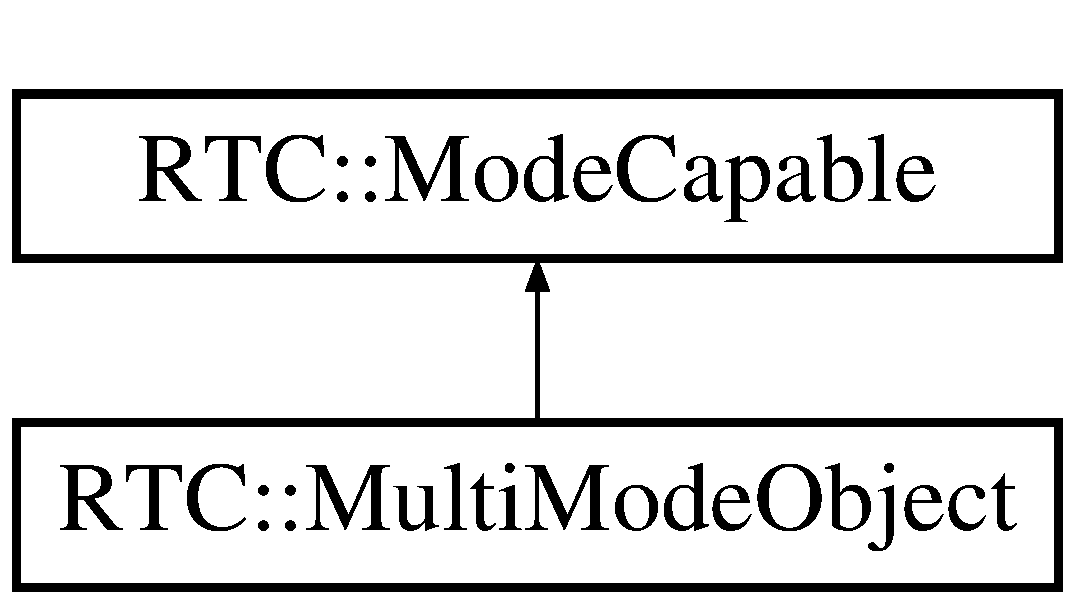
\includegraphics[height=2cm]{interfaceRTC_1_1ModeCapable}
\end{center}
\end{figure}
\subsection*{Public メソッド}
\begin{DoxyCompactItemize}
\item 
{\bf Mode} {\bf get\_\-default\_\-mode} ()
\item 
{\bf Mode} {\bf get\_\-current\_\-mode} ()
\item 
{\bf Mode} {\bf get\_\-current\_\-mode\_\-in\_\-context} (in {\bf ExecutionContext} exec\_\-context)
\item 
{\bf Mode} {\bf get\_\-pending\_\-mode} ()
\item 
{\bf Mode} {\bf get\_\-pending\_\-mode\_\-in\_\-context} (in {\bf ExecutionContext} exec\_\-context)
\item 
{\bf ReturnCode\_\-t} {\bf set\_\-mode} (in {\bf Mode} new\_\-mode, in boolean immediate)
\end{DoxyCompactItemize}


\subsection{関数}
\index{RTC::ModeCapable@{RTC::ModeCapable}!get\_\-current\_\-mode@{get\_\-current\_\-mode}}
\index{get\_\-current\_\-mode@{get\_\-current\_\-mode}!RTC::ModeCapable@{RTC::ModeCapable}}
\subsubsection[{get\_\-current\_\-mode}]{\setlength{\rightskip}{0pt plus 5cm}{\bf Mode} RTC::ModeCapable::get\_\-current\_\-mode ()}\label{interfaceRTC_1_1ModeCapable_a2adc0d8a34dc2a166fb29fc4fdf49133}
\index{RTC::ModeCapable@{RTC::ModeCapable}!get\_\-current\_\-mode\_\-in\_\-context@{get\_\-current\_\-mode\_\-in\_\-context}}
\index{get\_\-current\_\-mode\_\-in\_\-context@{get\_\-current\_\-mode\_\-in\_\-context}!RTC::ModeCapable@{RTC::ModeCapable}}
\subsubsection[{get\_\-current\_\-mode\_\-in\_\-context}]{\setlength{\rightskip}{0pt plus 5cm}{\bf Mode} RTC::ModeCapable::get\_\-current\_\-mode\_\-in\_\-context (in {\bf ExecutionContext} {\em exec\_\-context})}\label{interfaceRTC_1_1ModeCapable_a7ac136a5b2af22d96574d794f51dd4d5}
\index{RTC::ModeCapable@{RTC::ModeCapable}!get\_\-default\_\-mode@{get\_\-default\_\-mode}}
\index{get\_\-default\_\-mode@{get\_\-default\_\-mode}!RTC::ModeCapable@{RTC::ModeCapable}}
\subsubsection[{get\_\-default\_\-mode}]{\setlength{\rightskip}{0pt plus 5cm}{\bf Mode} RTC::ModeCapable::get\_\-default\_\-mode ()}\label{interfaceRTC_1_1ModeCapable_a5f086a75e4b1f22204bbb892b3062459}
\index{RTC::ModeCapable@{RTC::ModeCapable}!get\_\-pending\_\-mode@{get\_\-pending\_\-mode}}
\index{get\_\-pending\_\-mode@{get\_\-pending\_\-mode}!RTC::ModeCapable@{RTC::ModeCapable}}
\subsubsection[{get\_\-pending\_\-mode}]{\setlength{\rightskip}{0pt plus 5cm}{\bf Mode} RTC::ModeCapable::get\_\-pending\_\-mode ()}\label{interfaceRTC_1_1ModeCapable_a134b76f63a0f8003e983f17e9248c81b}
\index{RTC::ModeCapable@{RTC::ModeCapable}!get\_\-pending\_\-mode\_\-in\_\-context@{get\_\-pending\_\-mode\_\-in\_\-context}}
\index{get\_\-pending\_\-mode\_\-in\_\-context@{get\_\-pending\_\-mode\_\-in\_\-context}!RTC::ModeCapable@{RTC::ModeCapable}}
\subsubsection[{get\_\-pending\_\-mode\_\-in\_\-context}]{\setlength{\rightskip}{0pt plus 5cm}{\bf Mode} RTC::ModeCapable::get\_\-pending\_\-mode\_\-in\_\-context (in {\bf ExecutionContext} {\em exec\_\-context})}\label{interfaceRTC_1_1ModeCapable_a498bca5581602bc6421bfa9d3cde0f1d}
\index{RTC::ModeCapable@{RTC::ModeCapable}!set\_\-mode@{set\_\-mode}}
\index{set\_\-mode@{set\_\-mode}!RTC::ModeCapable@{RTC::ModeCapable}}
\subsubsection[{set\_\-mode}]{\setlength{\rightskip}{0pt plus 5cm}{\bf ReturnCode\_\-t} RTC::ModeCapable::set\_\-mode (in {\bf Mode} {\em new\_\-mode}, \/  in boolean {\em immediate})}\label{interfaceRTC_1_1ModeCapable_a07a6b11c57aef34b362ebd8c3bf9a462}


このインタフェースの説明は次のファイルから生成されました:\begin{DoxyCompactItemize}
\item 
{\bf RTC.idl}\end{DoxyCompactItemize}

\section{RTM::ModuleProfile Struct Reference}
\label{structRTM_1_1ModuleProfile}\index{RTM::ModuleProfile@{RTM::ModuleProfile}}


{\ttfamily import \char`\"{}Manager.idl\char`\"{};}

\subsection*{Public Attributes}
\begin{DoxyCompactItemize}
\item 
{\bf NVList} {\bf properties}
\end{DoxyCompactItemize}


\subsection{Member Data Documentation}
\index{RTM::ModuleProfile@{RTM::ModuleProfile}!properties@{properties}}
\index{properties@{properties}!RTM::ModuleProfile@{RTM::ModuleProfile}}
\subsubsection[{properties}]{\setlength{\rightskip}{0pt plus 5cm}{\bf NVList} {\bf RTM::ModuleProfile::properties}}\label{structRTM_1_1ModuleProfile_a50998e1c3e346b22e480cff93ff73eb1}


The documentation for this struct was generated from the following file:\begin{DoxyCompactItemize}
\item 
{\bf Manager.idl}\end{DoxyCompactItemize}

\section{インタフェース SDOPackage::Monitoring}
\label{interfaceSDOPackage_1_1Monitoring}\index{SDOPackage::Monitoring@{SDOPackage::Monitoring}}


{\ttfamily import \char`\"{}SDOPackage.idl\char`\"{};}



このインタフェースの説明は次のファイルから生成されました:\begin{DoxyCompactItemize}
\item 
{\bf SDOPackage.idl}\end{DoxyCompactItemize}

\section{インタフェース RTC::MultiModeComponentAction}
\label{interfaceRTC_1_1MultiModeComponentAction}\index{RTC::MultiModeComponentAction@{RTC::MultiModeComponentAction}}


{\ttfamily import \char`\"{}RTC.idl\char`\"{};}

RTC::MultiModeComponentActionに対する継承グラフ\begin{figure}[H]
\begin{center}
\leavevmode
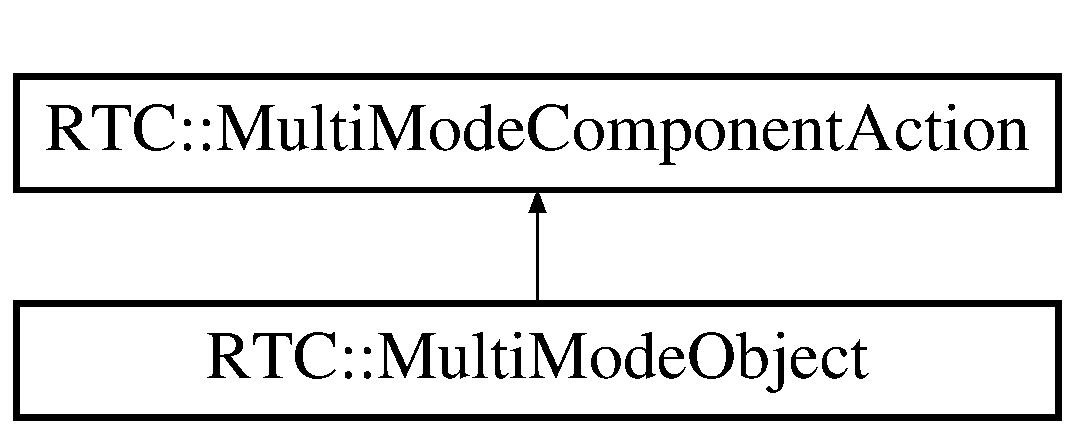
\includegraphics[height=2cm]{interfaceRTC_1_1MultiModeComponentAction}
\end{center}
\end{figure}
\subsection*{Public メソッド}
\begin{DoxyCompactItemize}
\item 
{\bf ReturnCode\_\-t} {\bf on\_\-mode\_\-changed} (in {\bf ExecutionContextHandle\_\-t} exec\_\-handle)
\end{DoxyCompactItemize}


\subsection{関数}
\index{RTC::MultiModeComponentAction@{RTC::MultiModeComponentAction}!on\_\-mode\_\-changed@{on\_\-mode\_\-changed}}
\index{on\_\-mode\_\-changed@{on\_\-mode\_\-changed}!RTC::MultiModeComponentAction@{RTC::MultiModeComponentAction}}
\subsubsection[{on\_\-mode\_\-changed}]{\setlength{\rightskip}{0pt plus 5cm}{\bf ReturnCode\_\-t} RTC::MultiModeComponentAction::on\_\-mode\_\-changed (in {\bf ExecutionContextHandle\_\-t} {\em exec\_\-handle})}\label{interfaceRTC_1_1MultiModeComponentAction_a0918cd39b3bfc001681ca40505304d7b}


このインタフェースの説明は次のファイルから生成されました:\begin{DoxyCompactItemize}
\item 
{\bf RTC.idl}\end{DoxyCompactItemize}

\section{RTC::MultiModeObject Interface Reference}
\label{interfaceRTC_1_1MultiModeObject}\index{RTC::MultiModeObject@{RTC::MultiModeObject}}


{\ttfamily import \char`\"{}RTC.idl\char`\"{};}

Inheritance diagram for RTC::MultiModeObject:\begin{figure}[H]
\begin{center}
\leavevmode
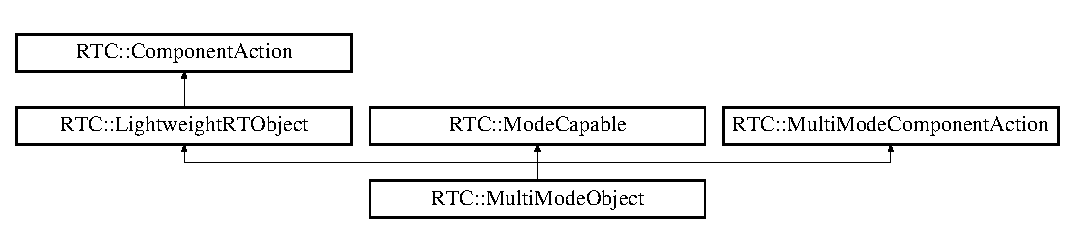
\includegraphics[height=2.69231cm]{interfaceRTC_1_1MultiModeObject}
\end{center}
\end{figure}
\subsection*{Public Member Functions}
\begin{DoxyCompactItemize}
\item 
{\bf ReturnCode\_\-t} {\bf initialize} ()
\begin{DoxyCompactList}\small\item\em initialize \item\end{DoxyCompactList}\item 
{\bf ReturnCode\_\-t} {\bf finalize} ()
\begin{DoxyCompactList}\small\item\em finalize \item\end{DoxyCompactList}\item 
boolean {\bf is\_\-alive} (in {\bf ExecutionContext} exec\_\-context)
\begin{DoxyCompactList}\small\item\em is\_\-alive \item\end{DoxyCompactList}\item 
{\bf ReturnCode\_\-t} {\bf exit} ()
\begin{DoxyCompactList}\small\item\em exit \item\end{DoxyCompactList}\item 
{\bf ExecutionContextHandle\_\-t} {\bf attach\_\-context} (in {\bf ExecutionContext} exec\_\-context)
\begin{DoxyCompactList}\small\item\em attach\_\-context \item\end{DoxyCompactList}\item 
{\bf ReturnCode\_\-t} {\bf detach\_\-context} (in {\bf ExecutionContextHandle\_\-t} exec\_\-handle)
\begin{DoxyCompactList}\small\item\em detach\_\-context \item\end{DoxyCompactList}\item 
{\bf ExecutionContext} {\bf get\_\-context} (in {\bf ExecutionContextHandle\_\-t} exec\_\-handle)
\begin{DoxyCompactList}\small\item\em get\_\-context \item\end{DoxyCompactList}\item 
{\bf ExecutionContextList} {\bf get\_\-owned\_\-contexts} ()
\begin{DoxyCompactList}\small\item\em get\_\-owned\_\-contexts \item\end{DoxyCompactList}\item 
{\bf ExecutionContextList} {\bf get\_\-participating\_\-contexts} ()
\begin{DoxyCompactList}\small\item\em $\ast$ get\_\-participating\_\-contexts \item\end{DoxyCompactList}\item 
{\bf ExecutionContextHandle\_\-t} {\bf get\_\-context\_\-handle} (in {\bf ExecutionContext} cxt)
\begin{DoxyCompactList}\small\item\em get\_\-context\_\-handle \item\end{DoxyCompactList}\item 
{\bf ReturnCode\_\-t} {\bf on\_\-initialize} ()
\begin{DoxyCompactList}\small\item\em on\_\-initialize \item\end{DoxyCompactList}\item 
{\bf ReturnCode\_\-t} {\bf on\_\-finalize} ()
\begin{DoxyCompactList}\small\item\em on\_\-finalize \item\end{DoxyCompactList}\item 
{\bf ReturnCode\_\-t} {\bf on\_\-startup} (in {\bf ExecutionContextHandle\_\-t} exec\_\-handle)
\begin{DoxyCompactList}\small\item\em on\_\-startup \item\end{DoxyCompactList}\item 
{\bf ReturnCode\_\-t} {\bf on\_\-shutdown} (in {\bf ExecutionContextHandle\_\-t} exec\_\-handle)
\begin{DoxyCompactList}\small\item\em on\_\-shutdown \item\end{DoxyCompactList}\item 
{\bf ReturnCode\_\-t} {\bf on\_\-activated} (in {\bf ExecutionContextHandle\_\-t} exec\_\-handle)
\begin{DoxyCompactList}\small\item\em on\_\-activated \item\end{DoxyCompactList}\item 
{\bf ReturnCode\_\-t} {\bf on\_\-deactivated} (in {\bf ExecutionContextHandle\_\-t} exec\_\-handle)
\begin{DoxyCompactList}\small\item\em on\_\-deactivated \item\end{DoxyCompactList}\item 
{\bf ReturnCode\_\-t} {\bf on\_\-aborting} (in {\bf ExecutionContextHandle\_\-t} exec\_\-handle)
\begin{DoxyCompactList}\small\item\em on\_\-aborting \item\end{DoxyCompactList}\item 
{\bf ReturnCode\_\-t} {\bf on\_\-error} (in {\bf ExecutionContextHandle\_\-t} exec\_\-handle)
\begin{DoxyCompactList}\small\item\em on\_\-error \item\end{DoxyCompactList}\item 
{\bf ReturnCode\_\-t} {\bf on\_\-reset} (in {\bf ExecutionContextHandle\_\-t} exec\_\-handle)
\begin{DoxyCompactList}\small\item\em on\_\-reset \item\end{DoxyCompactList}\item 
{\bf Mode} {\bf get\_\-default\_\-mode} ()
\begin{DoxyCompactList}\small\item\em get\_\-default\_\-mode \item\end{DoxyCompactList}\item 
{\bf Mode} {\bf get\_\-current\_\-mode} ()
\begin{DoxyCompactList}\small\item\em get\_\-current\_\-mode \item\end{DoxyCompactList}\item 
{\bf Mode} {\bf get\_\-current\_\-mode\_\-in\_\-context} (in {\bf ExecutionContext} exec\_\-context)
\begin{DoxyCompactList}\small\item\em get\_\-current\_\-mode\_\-in\_\-context \item\end{DoxyCompactList}\item 
{\bf Mode} {\bf get\_\-pending\_\-mode} ()
\begin{DoxyCompactList}\small\item\em get\_\-pending\_\-mode \item\end{DoxyCompactList}\item 
{\bf Mode} {\bf get\_\-pending\_\-mode\_\-in\_\-context} (in {\bf ExecutionContext} exec\_\-context)
\begin{DoxyCompactList}\small\item\em get\_\-pending\_\-mode\_\-in\_\-context \item\end{DoxyCompactList}\item 
{\bf ReturnCode\_\-t} {\bf set\_\-mode} (in {\bf Mode} new\_\-mode, in boolean immediate)
\begin{DoxyCompactList}\small\item\em set\_\-mode \item\end{DoxyCompactList}\item 
{\bf ReturnCode\_\-t} {\bf on\_\-mode\_\-changed} (in {\bf ExecutionContextHandle\_\-t} exec\_\-handle)
\begin{DoxyCompactList}\small\item\em on\_\-mode\_\-changed \item\end{DoxyCompactList}\end{DoxyCompactItemize}


\subsection{Member Function Documentation}
\index{RTC::MultiModeObject@{RTC::MultiModeObject}!attach\_\-context@{attach\_\-context}}
\index{attach\_\-context@{attach\_\-context}!RTC::MultiModeObject@{RTC::MultiModeObject}}
\subsubsection[{attach\_\-context}]{\setlength{\rightskip}{0pt plus 5cm}{\bf ExecutionContextHandle\_\-t} RTC::LightweightRTObject::attach\_\-context (in {\bf ExecutionContext} {\em exec\_\-context})\hspace{0.3cm}{\ttfamily  [inherited]}}\label{interfaceRTC_1_1LightweightRTObject_a48dbdbcac3254c29ad01d43a4ee5a00c}


attach\_\-context 

\subsection{Description}\label{namespaceRTC_Description}
Inform this \doxyref{RTC}{p.}{namespaceRTC} that it is participating in the given execution context. Return a handle that represents the association of this \doxyref{RTC}{p.}{namespaceRTC} with the context.\subsection{Semantics}\label{namespaceRTC_Semantics}
This operation is intended to be invoked by ExecutionContextOperations::add\_\-component (see Section 5.2.2.6.6). It is not intended for use by other clients. \index{RTC::MultiModeObject@{RTC::MultiModeObject}!detach\_\-context@{detach\_\-context}}
\index{detach\_\-context@{detach\_\-context}!RTC::MultiModeObject@{RTC::MultiModeObject}}
\subsubsection[{detach\_\-context}]{\setlength{\rightskip}{0pt plus 5cm}{\bf ReturnCode\_\-t} RTC::LightweightRTObject::detach\_\-context (in {\bf ExecutionContextHandle\_\-t} {\em exec\_\-handle})\hspace{0.3cm}{\ttfamily  [inherited]}}\label{interfaceRTC_1_1LightweightRTObject_a8eb94420ca08e8f7acaa778ed883b9a4}


detach\_\-context 

\subsection{Description}\label{namespaceRTC_Description}
Inform this \doxyref{RTC}{p.}{namespaceRTC} that it is no longer participating in the given execution context.\subsection{Semantics}\label{namespaceRTC_Semantics}
This operation is intended to be invoked by ExecutionContextOperations::remove\_\-component (see Section 5.2.2.6.7). It is not intended for use by other clients.\subsection{Constraints}\label{interfaceRTC_1_1LightweightRTObject_Constraints}

\begin{DoxyItemize}
\item This operation may not be invoked if this \doxyref{RTC}{p.}{namespaceRTC} is not already participating in the execution context. Such a call shall fail with ReturnCode\_\-t::PRECONDITION\_\-NOT\_\-MET.
\end{DoxyItemize}


\begin{DoxyItemize}
\item This operation may not be invoked if this \doxyref{RTC}{p.}{namespaceRTC} is Active in the indicated execution context. Otherwise, it shall fail with ReturnCode\_\-t::PRECONDITION\_\-NOT\_\-MET. 
\end{DoxyItemize}\index{RTC::MultiModeObject@{RTC::MultiModeObject}!exit@{exit}}
\index{exit@{exit}!RTC::MultiModeObject@{RTC::MultiModeObject}}
\subsubsection[{exit}]{\setlength{\rightskip}{0pt plus 5cm}{\bf ReturnCode\_\-t} RTC::LightweightRTObject::exit ()\hspace{0.3cm}{\ttfamily  [inherited]}}\label{interfaceRTC_1_1LightweightRTObject_a49bd940b6964fa80d696db15b45c2f87}


exit 

\subsection{Description}\label{namespaceRTC_Description}
Stop the RTC��s execution context(s) and finalize it along with its contents.\subsection{Semantics}\label{namespaceRTC_Semantics}
Any execution contexts for which the \doxyref{RTC}{p.}{namespaceRTC} is the owner shall be stopped. If the \doxyref{RTC}{p.}{namespaceRTC} participates in any execution contexts belonging to another \doxyref{RTC}{p.}{namespaceRTC} that contains it, directly or indirectly (i.e., the containing \doxyref{RTC}{p.}{namespaceRTC} is the owner of the \doxyref{ExecutionContext}{p.}{interfaceRTC_1_1ExecutionContext}), it shall be deactivated in those contexts. After the \doxyref{RTC}{p.}{namespaceRTC} is no longer Active in any Running execution context, it and any RTCs contained transitively within it shall be finalized.\subsection{Constraints}\label{interfaceRTC_1_1LightweightRTObject_Constraints}
An \doxyref{RTC}{p.}{namespaceRTC} cannot be exited if it has not yet been initialized. Any attempt to exit an \doxyref{RTC}{p.}{namespaceRTC} that is in the Created state shall fail with ReturnCode\_\-t::PRECONDITION\_\-NOT\_\-MET. \index{RTC::MultiModeObject@{RTC::MultiModeObject}!finalize@{finalize}}
\index{finalize@{finalize}!RTC::MultiModeObject@{RTC::MultiModeObject}}
\subsubsection[{finalize}]{\setlength{\rightskip}{0pt plus 5cm}{\bf ReturnCode\_\-t} RTC::LightweightRTObject::finalize ()\hspace{0.3cm}{\ttfamily  [inherited]}}\label{interfaceRTC_1_1LightweightRTObject_a23466f177b4289662ea035be831426ad}


finalize 

\subsection{Description}\label{namespaceRTC_Description}
Finalize the \doxyref{RTC}{p.}{namespaceRTC} that realizes this interface, preparing it for destruction.\subsection{Semantics}\label{namespaceRTC_Semantics}
This invocation of this operation shall result in the invocation of the callback \doxyref{ComponentAction::on\_\-finalize}{p.}{interfaceRTC_1_1ComponentAction_a9c9e2d638cd2b748609be8a23410aedc}\subsection{Constraints}\label{interfaceRTC_1_1LightweightRTObject_Constraints}

\begin{DoxyItemize}
\item An \doxyref{RTC}{p.}{namespaceRTC} may not be finalized while it is participating in any execution context. It must first be removed with ExecutionContextOperations::remove\_\-component. Otherwise, this operation shall fail with ReturnCode\_\-t::PRECONDITION\_\-NOT\_\-MET. See Figure 5.9.
\end{DoxyItemize}


\begin{DoxyItemize}
\item An \doxyref{RTC}{p.}{namespaceRTC} may not be finalized while it is in the Created state. Any attempt to invoke this operation while in that state shall fail with ReturnCode\_\-t::PRECONDITION\_\-NOT\_\-MET.
\end{DoxyItemize}


\begin{DoxyItemize}
\item Application developers are not expected to call this operation directly; it exists for use by the \doxyref{RTC}{p.}{namespaceRTC} infrastructure. 
\end{DoxyItemize}\index{RTC::MultiModeObject@{RTC::MultiModeObject}!get\_\-context@{get\_\-context}}
\index{get\_\-context@{get\_\-context}!RTC::MultiModeObject@{RTC::MultiModeObject}}
\subsubsection[{get\_\-context}]{\setlength{\rightskip}{0pt plus 5cm}{\bf ExecutionContext} RTC::LightweightRTObject::get\_\-context (in {\bf ExecutionContextHandle\_\-t} {\em exec\_\-handle})\hspace{0.3cm}{\ttfamily  [inherited]}}\label{interfaceRTC_1_1LightweightRTObject_a7bb123faf81bcb57542c3a17f10948d6}


get\_\-context 

\subsection{Description}\label{namespaceRTC_Description}
Obtain a reference to the execution context represented by the given handle.\subsection{Semantics}\label{namespaceRTC_Semantics}
The mapping from handle to context is specific to a particular \doxyref{RTC}{p.}{namespaceRTC} instance. The given handle must have been obtained by a previous call to attach\_\-context on this \doxyref{RTC}{p.}{namespaceRTC}. \index{RTC::MultiModeObject@{RTC::MultiModeObject}!get\_\-context\_\-handle@{get\_\-context\_\-handle}}
\index{get\_\-context\_\-handle@{get\_\-context\_\-handle}!RTC::MultiModeObject@{RTC::MultiModeObject}}
\subsubsection[{get\_\-context\_\-handle}]{\setlength{\rightskip}{0pt plus 5cm}{\bf ExecutionContextHandle\_\-t} RTC::LightweightRTObject::get\_\-context\_\-handle (in {\bf ExecutionContext} {\em cxt})\hspace{0.3cm}{\ttfamily  [inherited]}}\label{interfaceRTC_1_1LightweightRTObject_af54041744c01d68026aa200276e12f45}


get\_\-context\_\-handle 

\subsection{Description}\label{namespaceRTC_Description}
This operation returns a handle that is associated with the given execution context. \index{RTC::MultiModeObject@{RTC::MultiModeObject}!get\_\-current\_\-mode@{get\_\-current\_\-mode}}
\index{get\_\-current\_\-mode@{get\_\-current\_\-mode}!RTC::MultiModeObject@{RTC::MultiModeObject}}
\subsubsection[{get\_\-current\_\-mode}]{\setlength{\rightskip}{0pt plus 5cm}{\bf Mode} RTC::ModeCapable::get\_\-current\_\-mode ()\hspace{0.3cm}{\ttfamily  [inherited]}}\label{interfaceRTC_1_1ModeCapable_a2adc0d8a34dc2a166fb29fc4fdf49133}


get\_\-current\_\-mode 

\subsection{Description}\label{namespaceRTC_Description}
This operation shall return the last mode to have stabilized. If no mode has been explicitly set, the current mode shall be the default mode.\subsection{Constraints}\label{interfaceRTC_1_1LightweightRTObject_Constraints}

\begin{DoxyItemize}
\item This operation shall never return nil. 
\end{DoxyItemize}\index{RTC::MultiModeObject@{RTC::MultiModeObject}!get\_\-current\_\-mode\_\-in\_\-context@{get\_\-current\_\-mode\_\-in\_\-context}}
\index{get\_\-current\_\-mode\_\-in\_\-context@{get\_\-current\_\-mode\_\-in\_\-context}!RTC::MultiModeObject@{RTC::MultiModeObject}}
\subsubsection[{get\_\-current\_\-mode\_\-in\_\-context}]{\setlength{\rightskip}{0pt plus 5cm}{\bf Mode} RTC::ModeCapable::get\_\-current\_\-mode\_\-in\_\-context (in {\bf ExecutionContext} {\em exec\_\-context})\hspace{0.3cm}{\ttfamily  [inherited]}}\label{interfaceRTC_1_1ModeCapable_a7ac136a5b2af22d96574d794f51dd4d5}


get\_\-current\_\-mode\_\-in\_\-context 

\subsection{Description}\label{namespaceRTC_Description}
This operation returns the current mode of the component as seen by the indicated execution context.\subsection{Semantics}\label{namespaceRTC_Semantics}
The manner in which this property changes is described in Figure 5.26. \index{RTC::MultiModeObject@{RTC::MultiModeObject}!get\_\-default\_\-mode@{get\_\-default\_\-mode}}
\index{get\_\-default\_\-mode@{get\_\-default\_\-mode}!RTC::MultiModeObject@{RTC::MultiModeObject}}
\subsubsection[{get\_\-default\_\-mode}]{\setlength{\rightskip}{0pt plus 5cm}{\bf Mode} RTC::ModeCapable::get\_\-default\_\-mode ()\hspace{0.3cm}{\ttfamily  [inherited]}}\label{interfaceRTC_1_1ModeCapable_a5f086a75e4b1f22204bbb892b3062459}


get\_\-default\_\-mode 

\subsection{Description}\label{namespaceRTC_Description}
This operation shall return the mode in which the \doxyref{RTC}{p.}{namespaceRTC} shall be when no other mode has been set.\subsection{Constraints}\label{interfaceRTC_1_1LightweightRTObject_Constraints}

\begin{DoxyItemize}
\item This operation shall not return nil. 
\end{DoxyItemize}\index{RTC::MultiModeObject@{RTC::MultiModeObject}!get\_\-owned\_\-contexts@{get\_\-owned\_\-contexts}}
\index{get\_\-owned\_\-contexts@{get\_\-owned\_\-contexts}!RTC::MultiModeObject@{RTC::MultiModeObject}}
\subsubsection[{get\_\-owned\_\-contexts}]{\setlength{\rightskip}{0pt plus 5cm}{\bf ExecutionContextList} RTC::LightweightRTObject::get\_\-owned\_\-contexts ()\hspace{0.3cm}{\ttfamily  [inherited]}}\label{interfaceRTC_1_1LightweightRTObject_aea9dd2a447cc3ddc55f20aab698da408}


get\_\-owned\_\-contexts 

\subsection{Description}\label{namespaceRTC_Description}
This operation returns a list of all execution contexts owned by this \doxyref{RTC}{p.}{namespaceRTC}. \index{RTC::MultiModeObject@{RTC::MultiModeObject}!get\_\-participating\_\-contexts@{get\_\-participating\_\-contexts}}
\index{get\_\-participating\_\-contexts@{get\_\-participating\_\-contexts}!RTC::MultiModeObject@{RTC::MultiModeObject}}
\subsubsection[{get\_\-participating\_\-contexts}]{\setlength{\rightskip}{0pt plus 5cm}{\bf ExecutionContextList} RTC::LightweightRTObject::get\_\-participating\_\-contexts ()\hspace{0.3cm}{\ttfamily  [inherited]}}\label{interfaceRTC_1_1LightweightRTObject_af2224880b89275ecf82efad0999b022a}


$\ast$ get\_\-participating\_\-contexts 

\subsection{Description}\label{namespaceRTC_Description}
This operation returns a list of all execution contexts in which this \doxyref{RTC}{p.}{namespaceRTC} participates.\subsection{Semantics}\label{namespaceRTC_Semantics}
Each call to attach\_\-context causes the provided context to be added to this list. Each call to detach\_\-context causes the provided context to be removed from this list. \index{RTC::MultiModeObject@{RTC::MultiModeObject}!get\_\-pending\_\-mode@{get\_\-pending\_\-mode}}
\index{get\_\-pending\_\-mode@{get\_\-pending\_\-mode}!RTC::MultiModeObject@{RTC::MultiModeObject}}
\subsubsection[{get\_\-pending\_\-mode}]{\setlength{\rightskip}{0pt plus 5cm}{\bf Mode} RTC::ModeCapable::get\_\-pending\_\-mode ()\hspace{0.3cm}{\ttfamily  [inherited]}}\label{interfaceRTC_1_1ModeCapable_a134b76f63a0f8003e983f17e9248c81b}


get\_\-pending\_\-mode 

\subsection{Description}\label{namespaceRTC_Description}
This operation shall return the last mode to have been passed to set\_\-mode that has not yet stabilized. Once the RTC��s mode has stabilized, this operation shall return nil. \index{RTC::MultiModeObject@{RTC::MultiModeObject}!get\_\-pending\_\-mode\_\-in\_\-context@{get\_\-pending\_\-mode\_\-in\_\-context}}
\index{get\_\-pending\_\-mode\_\-in\_\-context@{get\_\-pending\_\-mode\_\-in\_\-context}!RTC::MultiModeObject@{RTC::MultiModeObject}}
\subsubsection[{get\_\-pending\_\-mode\_\-in\_\-context}]{\setlength{\rightskip}{0pt plus 5cm}{\bf Mode} RTC::ModeCapable::get\_\-pending\_\-mode\_\-in\_\-context (in {\bf ExecutionContext} {\em exec\_\-context})\hspace{0.3cm}{\ttfamily  [inherited]}}\label{interfaceRTC_1_1ModeCapable_a498bca5581602bc6421bfa9d3cde0f1d}


get\_\-pending\_\-mode\_\-in\_\-context 

\subsection{Description}\label{namespaceRTC_Description}
If the last mode to be requested by a call to set\_\-mode is different than the current mode as seen by the indicated execution context (see get\_\-current\_\-mode\_\-in\_\-context), this operation returns the former. If the requested mode has already been seen in that context, it returns nil.\subsection{Semantics}\label{namespaceRTC_Semantics}
See Figure 5.26 for a description of how the pending mode relates to the current mode within a given execution context. \index{RTC::MultiModeObject@{RTC::MultiModeObject}!initialize@{initialize}}
\index{initialize@{initialize}!RTC::MultiModeObject@{RTC::MultiModeObject}}
\subsubsection[{initialize}]{\setlength{\rightskip}{0pt plus 5cm}{\bf ReturnCode\_\-t} RTC::LightweightRTObject::initialize ()\hspace{0.3cm}{\ttfamily  [inherited]}}\label{interfaceRTC_1_1LightweightRTObject_afb28c4d97677804da09488578b840eb5}


initialize 

\subsection{Description}\label{namespaceRTC_Description}
Initialize the \doxyref{RTC}{p.}{namespaceRTC} that realizes this interface.\subsection{Semantics}\label{namespaceRTC_Semantics}
The invocation of this operation shall result in the invocation of the callback \doxyref{ComponentAction::on\_\-initialize}{p.}{interfaceRTC_1_1ComponentAction_a8703b183bc1bed9e2fd3ecac126cb231}.\subsection{Constraints}\label{interfaceRTC_1_1LightweightRTObject_Constraints}

\begin{DoxyItemize}
\item An \doxyref{RTC}{p.}{namespaceRTC} may be initialized only while it is in the Created state. Any attempt to invoke this operation while in another state shall fail with ReturnCode\_\-t::PRECONDITION\_\-NOT\_\-MET.
\item Application developers are not expected to call this operation directly; it exists for use by the \doxyref{RTC}{p.}{namespaceRTC} infrastructure. 
\end{DoxyItemize}\index{RTC::MultiModeObject@{RTC::MultiModeObject}!is\_\-alive@{is\_\-alive}}
\index{is\_\-alive@{is\_\-alive}!RTC::MultiModeObject@{RTC::MultiModeObject}}
\subsubsection[{is\_\-alive}]{\setlength{\rightskip}{0pt plus 5cm}boolean RTC::LightweightRTObject::is\_\-alive (in {\bf ExecutionContext} {\em exec\_\-context})\hspace{0.3cm}{\ttfamily  [inherited]}}\label{interfaceRTC_1_1LightweightRTObject_aa07c8c299b0addc49887508c1ee7be27}


is\_\-alive 

\subsection{Description}\label{namespaceRTC_Description}
A component is alive or not regardless of the execution context from which it is observed. However, whether or not it is Active, Inactive, or in Error is dependent on the execution context(s) (see Figure 5.7) in which it is running. That is, it may be Active in one context but Inactive in another. Therefore, this operation shall report whether this \doxyref{RTC}{p.}{namespaceRTC} is either Active, Inactive, or in Error; which of those states a component is in with respect to a particular context may be queried from the context itself. \index{RTC::MultiModeObject@{RTC::MultiModeObject}!on\_\-aborting@{on\_\-aborting}}
\index{on\_\-aborting@{on\_\-aborting}!RTC::MultiModeObject@{RTC::MultiModeObject}}
\subsubsection[{on\_\-aborting}]{\setlength{\rightskip}{0pt plus 5cm}{\bf ReturnCode\_\-t} RTC::ComponentAction::on\_\-aborting (in {\bf ExecutionContextHandle\_\-t} {\em exec\_\-handle})\hspace{0.3cm}{\ttfamily  [inherited]}}\label{interfaceRTC_1_1ComponentAction_a876e58ebcea16c307e131b3e6a58ddbe}


on\_\-aborting 

\subsection{Description}\label{namespaceRTC_Description}
The \doxyref{RTC}{p.}{namespaceRTC} is transitioning from the Active state to the Error state in some execution context.\subsection{Semantics}\label{namespaceRTC_Semantics}
This callback is invoked only a single time for time that the \doxyref{RTC}{p.}{namespaceRTC} transitions into the Error state from another state. This behavior is in contrast to that of on\_\-error. \index{RTC::MultiModeObject@{RTC::MultiModeObject}!on\_\-activated@{on\_\-activated}}
\index{on\_\-activated@{on\_\-activated}!RTC::MultiModeObject@{RTC::MultiModeObject}}
\subsubsection[{on\_\-activated}]{\setlength{\rightskip}{0pt plus 5cm}{\bf ReturnCode\_\-t} RTC::ComponentAction::on\_\-activated (in {\bf ExecutionContextHandle\_\-t} {\em exec\_\-handle})\hspace{0.3cm}{\ttfamily  [inherited]}}\label{interfaceRTC_1_1ComponentAction_a4f51f627067d0c54e89c4c0827fa6432}


on\_\-activated 

\subsection{Description}\label{namespaceRTC_Description}
The \doxyref{RTC}{p.}{namespaceRTC} has been activated in the given execution context. \index{RTC::MultiModeObject@{RTC::MultiModeObject}!on\_\-deactivated@{on\_\-deactivated}}
\index{on\_\-deactivated@{on\_\-deactivated}!RTC::MultiModeObject@{RTC::MultiModeObject}}
\subsubsection[{on\_\-deactivated}]{\setlength{\rightskip}{0pt plus 5cm}{\bf ReturnCode\_\-t} RTC::ComponentAction::on\_\-deactivated (in {\bf ExecutionContextHandle\_\-t} {\em exec\_\-handle})\hspace{0.3cm}{\ttfamily  [inherited]}}\label{interfaceRTC_1_1ComponentAction_aa5f9cfb9677ba685be333ad666c87f88}


on\_\-deactivated 

\subsection{Description}\label{namespaceRTC_Description}
The \doxyref{RTC}{p.}{namespaceRTC} has been deactivated in the given execution context. \index{RTC::MultiModeObject@{RTC::MultiModeObject}!on\_\-error@{on\_\-error}}
\index{on\_\-error@{on\_\-error}!RTC::MultiModeObject@{RTC::MultiModeObject}}
\subsubsection[{on\_\-error}]{\setlength{\rightskip}{0pt plus 5cm}{\bf ReturnCode\_\-t} RTC::ComponentAction::on\_\-error (in {\bf ExecutionContextHandle\_\-t} {\em exec\_\-handle})\hspace{0.3cm}{\ttfamily  [inherited]}}\label{interfaceRTC_1_1ComponentAction_a110fdde803e9b13f27308b897439962a}


on\_\-error 

\subsection{Description}\label{namespaceRTC_Description}
The \doxyref{RTC}{p.}{namespaceRTC} remains in the Error state.\subsection{Semantics}\label{namespaceRTC_Semantics}
If the \doxyref{RTC}{p.}{namespaceRTC} is in the Error state relative to some execution context when it would otherwise be invoked from that context (according to the context��s ExecutionKind), this callback shall be invoked instead. For example,


\begin{DoxyItemize}
\item If the ExecutionKind is PERIODIC, this operation shall be invoked in sorted order at the rate of the context instead of \doxyref{DataFlowComponentAction::on\_\-execute}{p.}{interfaceRTC_1_1DataFlowComponentAction_a70a1d7f32e03c719dd8949ea5d0be214} and on\_\-state\_\-update.
\end{DoxyItemize}


\begin{DoxyItemize}
\item If the ExecutionKind is EVENT\_\-DRIVEN, this operation shall be invoked whenever \doxyref{FsmParticipantAction::on\_\-action}{p.}{interfaceRTC_1_1FsmParticipantAction_ae627f5cdc59f586246bb2174797c7864} would otherwise have been invoked. 
\end{DoxyItemize}\index{RTC::MultiModeObject@{RTC::MultiModeObject}!on\_\-finalize@{on\_\-finalize}}
\index{on\_\-finalize@{on\_\-finalize}!RTC::MultiModeObject@{RTC::MultiModeObject}}
\subsubsection[{on\_\-finalize}]{\setlength{\rightskip}{0pt plus 5cm}{\bf ReturnCode\_\-t} RTC::ComponentAction::on\_\-finalize ()\hspace{0.3cm}{\ttfamily  [inherited]}}\label{interfaceRTC_1_1ComponentAction_a9c9e2d638cd2b748609be8a23410aedc}


on\_\-finalize 

\subsection{Description}\label{namespaceRTC_Description}
The \doxyref{RTC}{p.}{namespaceRTC} is being destroyed.\subsection{Semantics}\label{namespaceRTC_Semantics}
Any final RTC-\/specific tear-\/down logic should be performed here. \index{RTC::MultiModeObject@{RTC::MultiModeObject}!on\_\-initialize@{on\_\-initialize}}
\index{on\_\-initialize@{on\_\-initialize}!RTC::MultiModeObject@{RTC::MultiModeObject}}
\subsubsection[{on\_\-initialize}]{\setlength{\rightskip}{0pt plus 5cm}{\bf ReturnCode\_\-t} RTC::ComponentAction::on\_\-initialize ()\hspace{0.3cm}{\ttfamily  [inherited]}}\label{interfaceRTC_1_1ComponentAction_a8703b183bc1bed9e2fd3ecac126cb231}


on\_\-initialize 

\subsection{Description}\label{namespaceRTC_Description}
The \doxyref{RTC}{p.}{namespaceRTC} has been initialized and entered the Alive state.\subsection{Semantics}\label{namespaceRTC_Semantics}
Any RTC-\/specific initialization logic should be performed here. \index{RTC::MultiModeObject@{RTC::MultiModeObject}!on\_\-mode\_\-changed@{on\_\-mode\_\-changed}}
\index{on\_\-mode\_\-changed@{on\_\-mode\_\-changed}!RTC::MultiModeObject@{RTC::MultiModeObject}}
\subsubsection[{on\_\-mode\_\-changed}]{\setlength{\rightskip}{0pt plus 5cm}{\bf ReturnCode\_\-t} RTC::MultiModeComponentAction::on\_\-mode\_\-changed (in {\bf ExecutionContextHandle\_\-t} {\em exec\_\-handle})\hspace{0.3cm}{\ttfamily  [inherited]}}\label{interfaceRTC_1_1MultiModeComponentAction_a0918cd39b3bfc001681ca40505304d7b}


on\_\-mode\_\-changed 

\subsection{Description}\label{namespaceRTC_Description}
This callback is invoked each time the observed mode of a component has changed with respect to a particular execution context.\subsection{Semantics}\label{namespaceRTC_Semantics}
If the context is PERIODIC, this callback shall come before the next call to on\_\-execute (see Section 5.3.1.2.1) within that context. The new mode can be retrieved with get\_\-current\_\-mode\_\-in\_\-context. If the result is the same as the result of get\_\-current\_\-mode, the mode has stabilized. \index{RTC::MultiModeObject@{RTC::MultiModeObject}!on\_\-reset@{on\_\-reset}}
\index{on\_\-reset@{on\_\-reset}!RTC::MultiModeObject@{RTC::MultiModeObject}}
\subsubsection[{on\_\-reset}]{\setlength{\rightskip}{0pt plus 5cm}{\bf ReturnCode\_\-t} RTC::ComponentAction::on\_\-reset (in {\bf ExecutionContextHandle\_\-t} {\em exec\_\-handle})\hspace{0.3cm}{\ttfamily  [inherited]}}\label{interfaceRTC_1_1ComponentAction_adb0e61bff251337d79c7c7d050d8304e}


on\_\-reset 

\subsection{Description}\label{namespaceRTC_Description}
The \doxyref{RTC}{p.}{namespaceRTC} is in the Error state. An attempt is being made to recover it such that it can return to the Inactive state.\subsection{Semantics}\label{namespaceRTC_Semantics}
If the \doxyref{RTC}{p.}{namespaceRTC} was successfully recovered and can safely return to the Inactive state, this method shall complete with ReturnCode\_\-t::OK. Any other result shall indicate that the \doxyref{RTC}{p.}{namespaceRTC} should remain in the Error state. \index{RTC::MultiModeObject@{RTC::MultiModeObject}!on\_\-shutdown@{on\_\-shutdown}}
\index{on\_\-shutdown@{on\_\-shutdown}!RTC::MultiModeObject@{RTC::MultiModeObject}}
\subsubsection[{on\_\-shutdown}]{\setlength{\rightskip}{0pt plus 5cm}{\bf ReturnCode\_\-t} RTC::ComponentAction::on\_\-shutdown (in {\bf ExecutionContextHandle\_\-t} {\em exec\_\-handle})\hspace{0.3cm}{\ttfamily  [inherited]}}\label{interfaceRTC_1_1ComponentAction_accc47711344c811c9bdba0d66a3048f2}


on\_\-shutdown 

\subsection{Description}\label{namespaceRTC_Description}
The given execution context, in which the \doxyref{RTC}{p.}{namespaceRTC} is participating, has transitioned from Running to Stopped. \index{RTC::MultiModeObject@{RTC::MultiModeObject}!on\_\-startup@{on\_\-startup}}
\index{on\_\-startup@{on\_\-startup}!RTC::MultiModeObject@{RTC::MultiModeObject}}
\subsubsection[{on\_\-startup}]{\setlength{\rightskip}{0pt plus 5cm}{\bf ReturnCode\_\-t} RTC::ComponentAction::on\_\-startup (in {\bf ExecutionContextHandle\_\-t} {\em exec\_\-handle})\hspace{0.3cm}{\ttfamily  [inherited]}}\label{interfaceRTC_1_1ComponentAction_ac305f00c92f4650cf4fc798aac37eef2}


on\_\-startup 

\subsection{Description}\label{namespaceRTC_Description}
The given execution context, in which the \doxyref{RTC}{p.}{namespaceRTC} is participating, has transitioned from Stopped to Running. \index{RTC::MultiModeObject@{RTC::MultiModeObject}!set\_\-mode@{set\_\-mode}}
\index{set\_\-mode@{set\_\-mode}!RTC::MultiModeObject@{RTC::MultiModeObject}}
\subsubsection[{set\_\-mode}]{\setlength{\rightskip}{0pt plus 5cm}{\bf ReturnCode\_\-t} RTC::ModeCapable::set\_\-mode (in {\bf Mode} {\em new\_\-mode}, \/  in boolean {\em immediate})\hspace{0.3cm}{\ttfamily  [inherited]}}\label{interfaceRTC_1_1ModeCapable_a07a6b11c57aef34b362ebd8c3bf9a462}


set\_\-mode 

\subsection{Description}\label{namespaceRTC_Description}
This operation shall request that the \doxyref{RTC}{p.}{namespaceRTC} change to the indicated mode.\subsection{Semantics}\label{namespaceRTC_Semantics}
Usually, the new mode will be pending in each execution context in which the component executes until the next sample period (if the execution kind is PERIODIC); at that point it will become the current mode in that context and there will no longer be a pending mode. However, in some cases it is important for a mode change to take place immediately; for example, a serious fault has occurred and the component must enter an emergency mode to ensure fail-\/safe behavior in a safety-\/critical system. In such a case, immediate should be true and the mode change will take place in all contexts without waiting for the next sample period. 

The documentation for this interface was generated from the following file:\begin{DoxyCompactItemize}
\item 
{\bf RTC.idl}\end{DoxyCompactItemize}

\section{SDOPackage::NameValue Struct Reference}
\label{structSDOPackage_1_1NameValue}\index{SDOPackage::NameValue@{SDOPackage::NameValue}}


{\ttfamily import \char`\"{}SDOPackage.idl\char`\"{};}

\subsection*{Public Attributes}
\begin{DoxyCompactItemize}
\item 
string {\bf name}
\item 
any {\bf value}
\end{DoxyCompactItemize}


\subsection{Member Data Documentation}
\index{SDOPackage::NameValue@{SDOPackage::NameValue}!name@{name}}
\index{name@{name}!SDOPackage::NameValue@{SDOPackage::NameValue}}
\subsubsection[{name}]{\setlength{\rightskip}{0pt plus 5cm}string {\bf SDOPackage::NameValue::name}}\label{structSDOPackage_1_1NameValue_a4604ff503adb6aea4fc6908be13476ad}
\index{SDOPackage::NameValue@{SDOPackage::NameValue}!value@{value}}
\index{value@{value}!SDOPackage::NameValue@{SDOPackage::NameValue}}
\subsubsection[{value}]{\setlength{\rightskip}{0pt plus 5cm}any {\bf SDOPackage::NameValue::value}}\label{structSDOPackage_1_1NameValue_a0796af9c2444254bc9b5e9f63c182f00}


The documentation for this struct was generated from the following file:\begin{DoxyCompactItemize}
\item 
{\bf SDOPackage.idl}\end{DoxyCompactItemize}

\section{SDOPackage::Numeric Union Reference}
\label{unionSDOPackage_1_1Numeric}\index{SDOPackage::Numeric@{SDOPackage::Numeric}}


{\ttfamily import \char`\"{}SDOPackage.idl\char`\"{};}

\subsection*{Public Attributes}
\begin{DoxyCompactItemize}
\item 
short {\bf short\_\-value}
\item 
long {\bf long\_\-value}
\item 
float {\bf float\_\-value}
\item 
double {\bf double\_\-value}
\end{DoxyCompactItemize}


\subsection{Member Data Documentation}
\index{SDOPackage::Numeric@{SDOPackage::Numeric}!double\_\-value@{double\_\-value}}
\index{double\_\-value@{double\_\-value}!SDOPackage::Numeric@{SDOPackage::Numeric}}
\subsubsection[{double\_\-value}]{\setlength{\rightskip}{0pt plus 5cm}double {\bf SDOPackage::Numeric::double\_\-value}}\label{unionSDOPackage_1_1Numeric_aa6b082202442d38b557483d5d0d0d9ec}
\index{SDOPackage::Numeric@{SDOPackage::Numeric}!float\_\-value@{float\_\-value}}
\index{float\_\-value@{float\_\-value}!SDOPackage::Numeric@{SDOPackage::Numeric}}
\subsubsection[{float\_\-value}]{\setlength{\rightskip}{0pt plus 5cm}float {\bf SDOPackage::Numeric::float\_\-value}}\label{unionSDOPackage_1_1Numeric_af8a208ebea5bb57d21e277f45b638a90}
\index{SDOPackage::Numeric@{SDOPackage::Numeric}!long\_\-value@{long\_\-value}}
\index{long\_\-value@{long\_\-value}!SDOPackage::Numeric@{SDOPackage::Numeric}}
\subsubsection[{long\_\-value}]{\setlength{\rightskip}{0pt plus 5cm}long {\bf SDOPackage::Numeric::long\_\-value}}\label{unionSDOPackage_1_1Numeric_a925fa3b9f2f43b001183cdc5f6e60c91}
\index{SDOPackage::Numeric@{SDOPackage::Numeric}!short\_\-value@{short\_\-value}}
\index{short\_\-value@{short\_\-value}!SDOPackage::Numeric@{SDOPackage::Numeric}}
\subsubsection[{short\_\-value}]{\setlength{\rightskip}{0pt plus 5cm}short {\bf SDOPackage::Numeric::short\_\-value}}\label{unionSDOPackage_1_1Numeric_a37ea8e10da99b8d6147d59bb8bf1588b}


The documentation for this union was generated from the following file:\begin{DoxyCompactItemize}
\item 
{\bf SDOPackage.idl}\end{DoxyCompactItemize}

\section{インタフェース SDOPackage::Organization}
\label{interfaceSDOPackage_1_1Organization}\index{SDOPackage::Organization@{SDOPackage::Organization}}


{\ttfamily import \char`\"{}SDOPackage.idl\char`\"{};}

\subsection*{Public メソッド}
\begin{DoxyCompactItemize}
\item 
{\bf UniqueIdentifier} {\bf get\_\-organization\_\-id} ()  raises (InvalidParameter, NotAvailable, InternalError)
\item 
{\bf OrganizationProperty} {\bf get\_\-organization\_\-property} ()  raises (NotAvailable, InternalError)
\item 
any {\bf get\_\-organization\_\-property\_\-value} (in string name)  raises (InvalidParameter, NotAvailable, InternalError)
\item 
boolean {\bf add\_\-organization\_\-property} (in {\bf OrganizationProperty} organization\_\-property)  raises (InvalidParameter, NotAvailable, InternalError)
\item 
boolean {\bf set\_\-organization\_\-property\_\-value} (in string name, in any value)  raises (InvalidParameter, NotAvailable, InternalError)
\item 
boolean {\bf remove\_\-organization\_\-property} (in string name)  raises (InvalidParameter, NotAvailable, InternalError)
\item 
{\bf SDOSystemElement} {\bf get\_\-owner} ()  raises (NotAvailable, InternalError)
\item 
boolean {\bf set\_\-owner} (in {\bf SDOSystemElement} sdo)  raises (InvalidParameter, NotAvailable, InternalError)
\item 
{\bf SDOList} {\bf get\_\-members} ()  raises (NotAvailable, InternalError)
\item 
boolean {\bf set\_\-members} (in {\bf SDOList} sdos)  raises (InvalidParameter, NotAvailable, InternalError)
\item 
boolean {\bf add\_\-members} (in {\bf SDOList} sdo\_\-list)  raises (InvalidParameter, NotAvailable, InternalError)
\item 
boolean {\bf remove\_\-member} (in {\bf UniqueIdentifier} id)  raises (InvalidParameter, NotAvailable, InternalError)
\item 
{\bf DependencyType} {\bf get\_\-dependency} ()  raises (NotAvailable, InternalError)
\item 
boolean {\bf set\_\-dependency} (in {\bf DependencyType} dependency)  raises (NotAvailable, InternalError)
\end{DoxyCompactItemize}


\subsection{関数}
\index{SDOPackage::Organization@{SDOPackage::Organization}!add\_\-members@{add\_\-members}}
\index{add\_\-members@{add\_\-members}!SDOPackage::Organization@{SDOPackage::Organization}}
\subsubsection[{add\_\-members}]{\setlength{\rightskip}{0pt plus 5cm}boolean SDOPackage::Organization::add\_\-members (in {\bf SDOList} {\em sdo\_\-list})  raises (InvalidParameter, NotAvailable, InternalError)}\label{interfaceSDOPackage_1_1Organization_ac861802ce87ae4e9dfe69917a656ad83}
\index{SDOPackage::Organization@{SDOPackage::Organization}!add\_\-organization\_\-property@{add\_\-organization\_\-property}}
\index{add\_\-organization\_\-property@{add\_\-organization\_\-property}!SDOPackage::Organization@{SDOPackage::Organization}}
\subsubsection[{add\_\-organization\_\-property}]{\setlength{\rightskip}{0pt plus 5cm}boolean SDOPackage::Organization::add\_\-organization\_\-property (in {\bf OrganizationProperty} {\em organization\_\-property})  raises (InvalidParameter, NotAvailable, InternalError)}\label{interfaceSDOPackage_1_1Organization_a61424d3b010679e80c2544ee52dca3b6}
\index{SDOPackage::Organization@{SDOPackage::Organization}!get\_\-dependency@{get\_\-dependency}}
\index{get\_\-dependency@{get\_\-dependency}!SDOPackage::Organization@{SDOPackage::Organization}}
\subsubsection[{get\_\-dependency}]{\setlength{\rightskip}{0pt plus 5cm}{\bf DependencyType} SDOPackage::Organization::get\_\-dependency ()  raises (NotAvailable, InternalError)}\label{interfaceSDOPackage_1_1Organization_a49b9d3c850c65d27559fdc16b0f4f871}
\index{SDOPackage::Organization@{SDOPackage::Organization}!get\_\-members@{get\_\-members}}
\index{get\_\-members@{get\_\-members}!SDOPackage::Organization@{SDOPackage::Organization}}
\subsubsection[{get\_\-members}]{\setlength{\rightskip}{0pt plus 5cm}{\bf SDOList} SDOPackage::Organization::get\_\-members ()  raises (NotAvailable, InternalError)}\label{interfaceSDOPackage_1_1Organization_a98cbaec8451b195fb471da4c99fbfe8b}
\index{SDOPackage::Organization@{SDOPackage::Organization}!get\_\-organization\_\-id@{get\_\-organization\_\-id}}
\index{get\_\-organization\_\-id@{get\_\-organization\_\-id}!SDOPackage::Organization@{SDOPackage::Organization}}
\subsubsection[{get\_\-organization\_\-id}]{\setlength{\rightskip}{0pt plus 5cm}{\bf UniqueIdentifier} SDOPackage::Organization::get\_\-organization\_\-id ()  raises (InvalidParameter, NotAvailable, InternalError)}\label{interfaceSDOPackage_1_1Organization_adeab203a01786aeda24231e73fecd30e}
\index{SDOPackage::Organization@{SDOPackage::Organization}!get\_\-organization\_\-property@{get\_\-organization\_\-property}}
\index{get\_\-organization\_\-property@{get\_\-organization\_\-property}!SDOPackage::Organization@{SDOPackage::Organization}}
\subsubsection[{get\_\-organization\_\-property}]{\setlength{\rightskip}{0pt plus 5cm}{\bf OrganizationProperty} SDOPackage::Organization::get\_\-organization\_\-property ()  raises (NotAvailable, InternalError)}\label{interfaceSDOPackage_1_1Organization_a6211ce31022a4ca5b38e28833610fc5d}
\index{SDOPackage::Organization@{SDOPackage::Organization}!get\_\-organization\_\-property\_\-value@{get\_\-organization\_\-property\_\-value}}
\index{get\_\-organization\_\-property\_\-value@{get\_\-organization\_\-property\_\-value}!SDOPackage::Organization@{SDOPackage::Organization}}
\subsubsection[{get\_\-organization\_\-property\_\-value}]{\setlength{\rightskip}{0pt plus 5cm}any SDOPackage::Organization::get\_\-organization\_\-property\_\-value (in string {\em name})  raises (InvalidParameter, NotAvailable, InternalError)}\label{interfaceSDOPackage_1_1Organization_a1518d4e12866199506790ad7ec1035b1}
\index{SDOPackage::Organization@{SDOPackage::Organization}!get\_\-owner@{get\_\-owner}}
\index{get\_\-owner@{get\_\-owner}!SDOPackage::Organization@{SDOPackage::Organization}}
\subsubsection[{get\_\-owner}]{\setlength{\rightskip}{0pt plus 5cm}{\bf SDOSystemElement} SDOPackage::Organization::get\_\-owner ()  raises (NotAvailable, InternalError)}\label{interfaceSDOPackage_1_1Organization_a1b1f6113332162520169d4d0ed1d8eb7}
\index{SDOPackage::Organization@{SDOPackage::Organization}!remove\_\-member@{remove\_\-member}}
\index{remove\_\-member@{remove\_\-member}!SDOPackage::Organization@{SDOPackage::Organization}}
\subsubsection[{remove\_\-member}]{\setlength{\rightskip}{0pt plus 5cm}boolean SDOPackage::Organization::remove\_\-member (in {\bf UniqueIdentifier} {\em id})  raises (InvalidParameter, NotAvailable, InternalError)}\label{interfaceSDOPackage_1_1Organization_a8ba50b5da77d6354b2869e7da3bd7bfc}
\index{SDOPackage::Organization@{SDOPackage::Organization}!remove\_\-organization\_\-property@{remove\_\-organization\_\-property}}
\index{remove\_\-organization\_\-property@{remove\_\-organization\_\-property}!SDOPackage::Organization@{SDOPackage::Organization}}
\subsubsection[{remove\_\-organization\_\-property}]{\setlength{\rightskip}{0pt plus 5cm}boolean SDOPackage::Organization::remove\_\-organization\_\-property (in string {\em name})  raises (InvalidParameter, NotAvailable, InternalError)}\label{interfaceSDOPackage_1_1Organization_a16712f0f6513b226cb5428f89a63c00a}
\index{SDOPackage::Organization@{SDOPackage::Organization}!set\_\-dependency@{set\_\-dependency}}
\index{set\_\-dependency@{set\_\-dependency}!SDOPackage::Organization@{SDOPackage::Organization}}
\subsubsection[{set\_\-dependency}]{\setlength{\rightskip}{0pt plus 5cm}boolean SDOPackage::Organization::set\_\-dependency (in {\bf DependencyType} {\em dependency})  raises (NotAvailable, InternalError)}\label{interfaceSDOPackage_1_1Organization_ab0d8070846673145e46508640e8d36e1}
\index{SDOPackage::Organization@{SDOPackage::Organization}!set\_\-members@{set\_\-members}}
\index{set\_\-members@{set\_\-members}!SDOPackage::Organization@{SDOPackage::Organization}}
\subsubsection[{set\_\-members}]{\setlength{\rightskip}{0pt plus 5cm}boolean SDOPackage::Organization::set\_\-members (in {\bf SDOList} {\em sdos})  raises (InvalidParameter, NotAvailable, InternalError)}\label{interfaceSDOPackage_1_1Organization_a4b4dc833033b64539eb3ce92485b3e41}
\index{SDOPackage::Organization@{SDOPackage::Organization}!set\_\-organization\_\-property\_\-value@{set\_\-organization\_\-property\_\-value}}
\index{set\_\-organization\_\-property\_\-value@{set\_\-organization\_\-property\_\-value}!SDOPackage::Organization@{SDOPackage::Organization}}
\subsubsection[{set\_\-organization\_\-property\_\-value}]{\setlength{\rightskip}{0pt plus 5cm}boolean SDOPackage::Organization::set\_\-organization\_\-property\_\-value (in string {\em name}, \/  in any {\em value})  raises (InvalidParameter, NotAvailable, InternalError)}\label{interfaceSDOPackage_1_1Organization_a4d38682f8fdd019d229aee109f2de1f1}
\index{SDOPackage::Organization@{SDOPackage::Organization}!set\_\-owner@{set\_\-owner}}
\index{set\_\-owner@{set\_\-owner}!SDOPackage::Organization@{SDOPackage::Organization}}
\subsubsection[{set\_\-owner}]{\setlength{\rightskip}{0pt plus 5cm}boolean SDOPackage::Organization::set\_\-owner (in {\bf SDOSystemElement} {\em sdo})  raises (InvalidParameter, NotAvailable, InternalError)}\label{interfaceSDOPackage_1_1Organization_a8b747ff46647c4d2e28df2e9b9de325b}


このインタフェースの説明は次のファイルから生成されました:\begin{DoxyCompactItemize}
\item 
{\bf SDOPackage.idl}\end{DoxyCompactItemize}

\section{SDOPackage::OrganizationProperty Struct Reference}
\label{structSDOPackage_1_1OrganizationProperty}\index{SDOPackage::OrganizationProperty@{SDOPackage::OrganizationProperty}}


{\ttfamily import \char`\"{}SDOPackage.idl\char`\"{};}

\subsection*{Public Attributes}
\begin{DoxyCompactItemize}
\item 
{\bf NVList} {\bf properties}
\end{DoxyCompactItemize}


\subsection{Member Data Documentation}
\index{SDOPackage::OrganizationProperty@{SDOPackage::OrganizationProperty}!properties@{properties}}
\index{properties@{properties}!SDOPackage::OrganizationProperty@{SDOPackage::OrganizationProperty}}
\subsubsection[{properties}]{\setlength{\rightskip}{0pt plus 5cm}{\bf NVList} {\bf SDOPackage::OrganizationProperty::properties}}\label{structSDOPackage_1_1OrganizationProperty_a7ffebfa961644064d0051782634c2554}


The documentation for this struct was generated from the following file:\begin{DoxyCompactItemize}
\item 
{\bf SDOPackage.idl}\end{DoxyCompactItemize}

\section{インタフェース OpenRTM::OutPortCdr}
\label{interfaceOpenRTM_1_1OutPortCdr}\index{OpenRTM::OutPortCdr@{OpenRTM::OutPortCdr}}


{\ttfamily import \char`\"{}DataPort.idl\char`\"{};}

\subsection*{Public メソッド}
\begin{DoxyCompactItemize}
\item 
{\bf PortStatus} {\bf get} (out {\bf CdrData} data)
\end{DoxyCompactItemize}


\subsection{関数}
\index{OpenRTM::OutPortCdr@{OpenRTM::OutPortCdr}!get@{get}}
\index{get@{get}!OpenRTM::OutPortCdr@{OpenRTM::OutPortCdr}}
\subsubsection[{get}]{\setlength{\rightskip}{0pt plus 5cm}{\bf PortStatus} OpenRTM::OutPortCdr::get (out {\bf CdrData} {\em data})}\label{interfaceOpenRTM_1_1OutPortCdr_a28570fbad908079a88059498845aa417}


このインタフェースの説明は次のファイルから生成されました:\begin{DoxyCompactItemize}
\item 
{\bf DataPort.idl}\end{DoxyCompactItemize}

\section{SDOPackage::Parameter Struct Reference}
\label{structSDOPackage_1_1Parameter}\index{SDOPackage::Parameter@{SDOPackage::Parameter}}


{\ttfamily import \char`\"{}SDOPackage.idl\char`\"{};}

\subsection*{Public Attributes}
\begin{DoxyCompactItemize}
\item 
string {\bf name}
\item 
TypeCode {\bf type}
\item 
{\bf AllowedValues} {\bf allowed\_\-values}
\end{DoxyCompactItemize}


\subsection{Member Data Documentation}
\index{SDOPackage::Parameter@{SDOPackage::Parameter}!allowed\_\-values@{allowed\_\-values}}
\index{allowed\_\-values@{allowed\_\-values}!SDOPackage::Parameter@{SDOPackage::Parameter}}
\subsubsection[{allowed\_\-values}]{\setlength{\rightskip}{0pt plus 5cm}{\bf AllowedValues} {\bf SDOPackage::Parameter::allowed\_\-values}}\label{structSDOPackage_1_1Parameter_a81cafbb66579be6e62740aa4d093b8be}
\index{SDOPackage::Parameter@{SDOPackage::Parameter}!name@{name}}
\index{name@{name}!SDOPackage::Parameter@{SDOPackage::Parameter}}
\subsubsection[{name}]{\setlength{\rightskip}{0pt plus 5cm}string {\bf SDOPackage::Parameter::name}}\label{structSDOPackage_1_1Parameter_a0da7260b28bd3569dad58dc7c5bba457}
\index{SDOPackage::Parameter@{SDOPackage::Parameter}!type@{type}}
\index{type@{type}!SDOPackage::Parameter@{SDOPackage::Parameter}}
\subsubsection[{type}]{\setlength{\rightskip}{0pt plus 5cm}TypeCode {\bf SDOPackage::Parameter::type}}\label{structSDOPackage_1_1Parameter_a013f778942e59807be89122000bb7f25}


The documentation for this struct was generated from the following file:\begin{DoxyCompactItemize}
\item 
{\bf SDOPackage.idl}\end{DoxyCompactItemize}

\section{RTC::PortInterfaceProfile Struct Reference}
\label{structRTC_1_1PortInterfaceProfile}\index{RTC::PortInterfaceProfile@{RTC::PortInterfaceProfile}}


\doxyref{PortInterfaceProfile}{p.}{structRTC_1_1PortInterfaceProfile}.  




{\ttfamily import \char`\"{}RTC.idl\char`\"{};}

\subsection*{Public Attributes}
\begin{DoxyCompactItemize}
\item 
string {\bf instance\_\-name}
\begin{DoxyCompactList}\small\item\em instance\_\-name \item\end{DoxyCompactList}\item 
string {\bf type\_\-name}
\begin{DoxyCompactList}\small\item\em type\_\-name \item\end{DoxyCompactList}\item 
{\bf PortInterfacePolarity} {\bf polarity}
\begin{DoxyCompactList}\small\item\em polarity \item\end{DoxyCompactList}\end{DoxyCompactItemize}


\subsection{Detailed Description}
\doxyref{PortInterfaceProfile}{p.}{structRTC_1_1PortInterfaceProfile}. \subsection{Description}\label{namespaceRTC_Description}
\doxyref{PortInterfaceProfile}{p.}{structRTC_1_1PortInterfaceProfile} describes an instance of a particular interface as it is exposed by a particular port. These objects are referred to below as the \char`\"{}target interface\char`\"{} and \char`\"{}target
 port\char`\"{} respectively. 

\subsection{Member Data Documentation}
\index{RTC::PortInterfaceProfile@{RTC::PortInterfaceProfile}!instance\_\-name@{instance\_\-name}}
\index{instance\_\-name@{instance\_\-name}!RTC::PortInterfaceProfile@{RTC::PortInterfaceProfile}}
\subsubsection[{instance\_\-name}]{\setlength{\rightskip}{0pt plus 5cm}string {\bf RTC::PortInterfaceProfile::instance\_\-name}}\label{structRTC_1_1PortInterfaceProfile_a725784d1451e8f16269c57b571aa0ed6}


instance\_\-name 

\subsection{Description}\label{namespaceRTC_Description}
This attribute stores the name of the target interface instance. \index{RTC::PortInterfaceProfile@{RTC::PortInterfaceProfile}!polarity@{polarity}}
\index{polarity@{polarity}!RTC::PortInterfaceProfile@{RTC::PortInterfaceProfile}}
\subsubsection[{polarity}]{\setlength{\rightskip}{0pt plus 5cm}{\bf PortInterfacePolarity} {\bf RTC::PortInterfaceProfile::polarity}}\label{structRTC_1_1PortInterfaceProfile_a65e7b1f54dc9334341257609cc70a9b6}


polarity 

\subsection{Description}\label{namespaceRTC_Description}
This attribute indicates whether the target interface instance is provided or required by the \doxyref{RTC}{p.}{namespaceRTC}. \index{RTC::PortInterfaceProfile@{RTC::PortInterfaceProfile}!type\_\-name@{type\_\-name}}
\index{type\_\-name@{type\_\-name}!RTC::PortInterfaceProfile@{RTC::PortInterfaceProfile}}
\subsubsection[{type\_\-name}]{\setlength{\rightskip}{0pt plus 5cm}string {\bf RTC::PortInterfaceProfile::type\_\-name}}\label{structRTC_1_1PortInterfaceProfile_ad5ffa44cfad5a86628ddeea5a294d801}


type\_\-name 

\subsection{Description}\label{namespaceRTC_Description}
This attribute stores the name of the target interface type. 

The documentation for this struct was generated from the following file:\begin{DoxyCompactItemize}
\item 
{\bf RTC.idl}\end{DoxyCompactItemize}

\section{構造体 RTC::PortProfile}
\label{structRTC_1_1PortProfile}\index{RTC::PortProfile@{RTC::PortProfile}}


{\ttfamily import \char`\"{}RTC.idl\char`\"{};}

\subsection*{Public 変数}
\begin{DoxyCompactItemize}
\item 
string {\bf name}
\item 
{\bf PortInterfaceProfileList} {\bf interfaces}
\item 
{\bf PortService} {\bf port\_\-ref}
\item 
{\bf ConnectorProfileList} {\bf connector\_\-profiles}
\item 
{\bf RTObject} {\bf owner}
\item 
{\bf NVList} {\bf properties}
\end{DoxyCompactItemize}


\subsection{変数}
\index{RTC::PortProfile@{RTC::PortProfile}!connector\_\-profiles@{connector\_\-profiles}}
\index{connector\_\-profiles@{connector\_\-profiles}!RTC::PortProfile@{RTC::PortProfile}}
\subsubsection[{connector\_\-profiles}]{\setlength{\rightskip}{0pt plus 5cm}{\bf ConnectorProfileList} {\bf RTC::PortProfile::connector\_\-profiles}}\label{structRTC_1_1PortProfile_a2222e576d0995c9a84663fb485f24aff}
\index{RTC::PortProfile@{RTC::PortProfile}!interfaces@{interfaces}}
\index{interfaces@{interfaces}!RTC::PortProfile@{RTC::PortProfile}}
\subsubsection[{interfaces}]{\setlength{\rightskip}{0pt plus 5cm}{\bf PortInterfaceProfileList} {\bf RTC::PortProfile::interfaces}}\label{structRTC_1_1PortProfile_ab9cda86e55b788ed3dc7d793d9849dab}
\index{RTC::PortProfile@{RTC::PortProfile}!name@{name}}
\index{name@{name}!RTC::PortProfile@{RTC::PortProfile}}
\subsubsection[{name}]{\setlength{\rightskip}{0pt plus 5cm}string {\bf RTC::PortProfile::name}}\label{structRTC_1_1PortProfile_aad548e10074a048a2d37282d75373d83}
\index{RTC::PortProfile@{RTC::PortProfile}!owner@{owner}}
\index{owner@{owner}!RTC::PortProfile@{RTC::PortProfile}}
\subsubsection[{owner}]{\setlength{\rightskip}{0pt plus 5cm}{\bf RTObject} {\bf RTC::PortProfile::owner}}\label{structRTC_1_1PortProfile_a91b5c831f6c0dff96d0aa69d7cd84392}
\index{RTC::PortProfile@{RTC::PortProfile}!port\_\-ref@{port\_\-ref}}
\index{port\_\-ref@{port\_\-ref}!RTC::PortProfile@{RTC::PortProfile}}
\subsubsection[{port\_\-ref}]{\setlength{\rightskip}{0pt plus 5cm}{\bf PortService} {\bf RTC::PortProfile::port\_\-ref}}\label{structRTC_1_1PortProfile_aa0ed1c408a064f19080bc0a21a96bc43}
\index{RTC::PortProfile@{RTC::PortProfile}!properties@{properties}}
\index{properties@{properties}!RTC::PortProfile@{RTC::PortProfile}}
\subsubsection[{properties}]{\setlength{\rightskip}{0pt plus 5cm}{\bf NVList} {\bf RTC::PortProfile::properties}}\label{structRTC_1_1PortProfile_aa9b72d4c51a62eab04ac2c701e39eaeb}


この構造体の説明は次のファイルから生成されました:\begin{DoxyCompactItemize}
\item 
{\bf RTC.idl}\end{DoxyCompactItemize}

\section{RTC::PortService Interface Reference}
\label{interfaceRTC_1_1PortService}\index{RTC::PortService@{RTC::PortService}}


\doxyref{PortService}{p.}{interfaceRTC_1_1PortService}.  




{\ttfamily import \char`\"{}RTC.idl\char`\"{};}

Inheritance diagram for RTC::PortService:\begin{figure}[H]
\begin{center}
\leavevmode
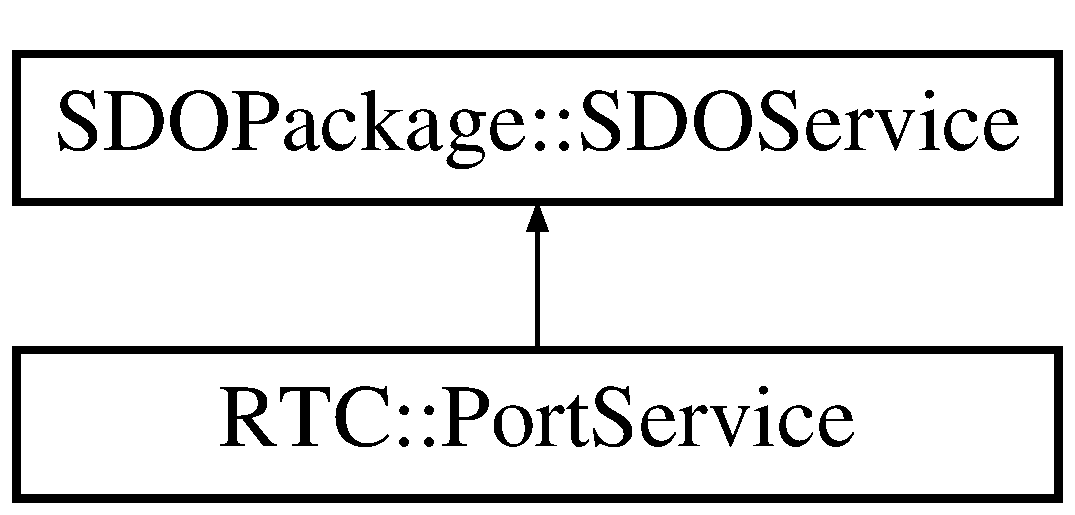
\includegraphics[height=2cm]{interfaceRTC_1_1PortService}
\end{center}
\end{figure}
\subsection*{Public Member Functions}
\begin{DoxyCompactItemize}
\item 
{\bf PortProfile} {\bf get\_\-port\_\-profile} ()
\begin{DoxyCompactList}\small\item\em get\_\-port\_\-profile \item\end{DoxyCompactList}\item 
{\bf ConnectorProfileList} {\bf get\_\-connector\_\-profiles} ()
\begin{DoxyCompactList}\small\item\em get\_\-connector\_\-profiles \item\end{DoxyCompactList}\item 
{\bf ConnectorProfile} {\bf get\_\-connector\_\-profile} (in {\bf UniqueIdentifier} connector\_\-id)
\begin{DoxyCompactList}\small\item\em get\_\-connector\_\-profiles \item\end{DoxyCompactList}\item 
{\bf ReturnCode\_\-t} {\bf connect} (inout {\bf ConnectorProfile} connector\_\-profile)
\begin{DoxyCompactList}\small\item\em connect \item\end{DoxyCompactList}\item 
{\bf ReturnCode\_\-t} {\bf disconnect} (in {\bf UniqueIdentifier} connector\_\-id)
\begin{DoxyCompactList}\small\item\em disconnect \item\end{DoxyCompactList}\item 
{\bf ReturnCode\_\-t} {\bf disconnect\_\-all} ()
\begin{DoxyCompactList}\small\item\em disconnect\_\-all \item\end{DoxyCompactList}\item 
{\bf ReturnCode\_\-t} {\bf notify\_\-connect} (inout {\bf ConnectorProfile} connector\_\-profile)
\begin{DoxyCompactList}\small\item\em notify\_\-connect \item\end{DoxyCompactList}\item 
{\bf ReturnCode\_\-t} {\bf notify\_\-disconnect} (in {\bf UniqueIdentifier} connector\_\-id)
\begin{DoxyCompactList}\small\item\em notify\_\-disconnect \item\end{DoxyCompactList}\end{DoxyCompactItemize}


\subsection{Detailed Description}
\doxyref{PortService}{p.}{interfaceRTC_1_1PortService}. \subsection{Description}\label{namespaceRTC_Description}
An instance of the \doxyref{PortService}{p.}{interfaceRTC_1_1PortService} interface represents a port (i.e., UML::Composite Structures::Ports::Port) of an \doxyref{RTC}{p.}{namespaceRTC}. It provides operations that allow it to be connected to and disconnected from other ports.\subsection{Semantics}\label{namespaceRTC_Semantics}
A port service can support unidirectional or bidirectional communication. A port service may allow for a service-\/oriented connection, in which other connected ports, invoke methods on it. It may also allow for a data-\/centric connection, in which data values are streamed in or out. In either case, the connection is described by an instance of \doxyref{ConnectorProfile}{p.}{structRTC_1_1ConnectorProfile}. However, the behavioral contracts of such connections are dependent on the interfaces exposed by the ports and are not described normatively by this specification. 

\subsection{Member Function Documentation}
\index{RTC::PortService@{RTC::PortService}!connect@{connect}}
\index{connect@{connect}!RTC::PortService@{RTC::PortService}}
\subsubsection[{connect}]{\setlength{\rightskip}{0pt plus 5cm}{\bf ReturnCode\_\-t} RTC::PortService::connect (inout {\bf ConnectorProfile} {\em connector\_\-profile})}\label{interfaceRTC_1_1PortService_a7d1a4236a839d99274f2ba0c25858996}


connect 

\subsection{Description}\label{namespaceRTC_Description}
This operation establishes connection between this port and the peer ports according to given ConnectionProfile.\subsection{Semantics}\label{namespaceRTC_Semantics}
A \doxyref{ConnectorProfile}{p.}{structRTC_1_1ConnectorProfile} has a sequence of port references. This port invokes the notify\_\-connect operation of one of the ports included in the sequence. It follows that the notification of connection is propagated by the notify\_\-connect operation with \doxyref{ConnectorProfile}{p.}{structRTC_1_1ConnectorProfile}. This operation returns \doxyref{ConnectorProfile}{p.}{structRTC_1_1ConnectorProfile} return value and returns ReturnCode\_\-t as return codes. \index{RTC::PortService@{RTC::PortService}!disconnect@{disconnect}}
\index{disconnect@{disconnect}!RTC::PortService@{RTC::PortService}}
\subsubsection[{disconnect}]{\setlength{\rightskip}{0pt plus 5cm}{\bf ReturnCode\_\-t} RTC::PortService::disconnect (in {\bf UniqueIdentifier} {\em connector\_\-id})}\label{interfaceRTC_1_1PortService_ad6a9a46323d4c2e49131c3ec5717d9e3}


disconnect 

\subsection{Description}\label{namespaceRTC_Description}
This operation destroys the connection between this port and its peer ports using the ID that was given when the connection was established.\subsection{Semantics}\label{namespaceRTC_Semantics}
This port invokes the notify\_\-disconnect operation of one of the ports included in the sequence of the \doxyref{ConnectorProfile}{p.}{structRTC_1_1ConnectorProfile} stored when the connection was established. The notification of disconnection is propagated by the notify\_\-disconnect operation. \index{RTC::PortService@{RTC::PortService}!disconnect\_\-all@{disconnect\_\-all}}
\index{disconnect\_\-all@{disconnect\_\-all}!RTC::PortService@{RTC::PortService}}
\subsubsection[{disconnect\_\-all}]{\setlength{\rightskip}{0pt plus 5cm}{\bf ReturnCode\_\-t} RTC::PortService::disconnect\_\-all ()}\label{interfaceRTC_1_1PortService_a4d1bf316f490f0cc29cc10ff4183dac5}


disconnect\_\-all 

\subsection{Description}\label{namespaceRTC_Description}
This operation destroys all connection channels owned by the \doxyref{PortService}{p.}{interfaceRTC_1_1PortService}. \index{RTC::PortService@{RTC::PortService}!get\_\-connector\_\-profile@{get\_\-connector\_\-profile}}
\index{get\_\-connector\_\-profile@{get\_\-connector\_\-profile}!RTC::PortService@{RTC::PortService}}
\subsubsection[{get\_\-connector\_\-profile}]{\setlength{\rightskip}{0pt plus 5cm}{\bf ConnectorProfile} RTC::PortService::get\_\-connector\_\-profile (in {\bf UniqueIdentifier} {\em connector\_\-id})}\label{interfaceRTC_1_1PortService_a7766a1632deded815a2a312148933057}


get\_\-connector\_\-profiles 

\subsection{Description}\label{namespaceRTC_Description}
This operation returns a list of the ConnectorProfiles of the \doxyref{PortService}{p.}{interfaceRTC_1_1PortService}. \index{RTC::PortService@{RTC::PortService}!get\_\-connector\_\-profiles@{get\_\-connector\_\-profiles}}
\index{get\_\-connector\_\-profiles@{get\_\-connector\_\-profiles}!RTC::PortService@{RTC::PortService}}
\subsubsection[{get\_\-connector\_\-profiles}]{\setlength{\rightskip}{0pt plus 5cm}{\bf ConnectorProfileList} RTC::PortService::get\_\-connector\_\-profiles ()}\label{interfaceRTC_1_1PortService_a2f1edec9892d8228960f3930ca18393a}


get\_\-connector\_\-profiles 

\subsection{Description}\label{namespaceRTC_Description}
This operation returns a list of the ConnectorProfiles of the \doxyref{PortService}{p.}{interfaceRTC_1_1PortService}. \index{RTC::PortService@{RTC::PortService}!get\_\-port\_\-profile@{get\_\-port\_\-profile}}
\index{get\_\-port\_\-profile@{get\_\-port\_\-profile}!RTC::PortService@{RTC::PortService}}
\subsubsection[{get\_\-port\_\-profile}]{\setlength{\rightskip}{0pt plus 5cm}{\bf PortProfile} RTC::PortService::get\_\-port\_\-profile ()}\label{interfaceRTC_1_1PortService_a90d7e716d7c9ca13bde3767b6d138e53}


get\_\-port\_\-profile 

\subsection{Description}\label{namespaceRTC_Description}
This operation returns the \doxyref{PortProfile}{p.}{structRTC_1_1PortProfile} of the \doxyref{PortService}{p.}{interfaceRTC_1_1PortService}. \index{RTC::PortService@{RTC::PortService}!notify\_\-connect@{notify\_\-connect}}
\index{notify\_\-connect@{notify\_\-connect}!RTC::PortService@{RTC::PortService}}
\subsubsection[{notify\_\-connect}]{\setlength{\rightskip}{0pt plus 5cm}{\bf ReturnCode\_\-t} RTC::PortService::notify\_\-connect (inout {\bf ConnectorProfile} {\em connector\_\-profile})}\label{interfaceRTC_1_1PortService_af021417d7d9c8966dd346d7193d5219b}


notify\_\-connect 

\subsection{Description}\label{namespaceRTC_Description}
This operation notifies this \doxyref{PortService}{p.}{interfaceRTC_1_1PortService} of the connection between its corresponding port and the other ports and propagates the given ConnectionProfile.\subsection{Semantics}\label{namespaceRTC_Semantics}
A \doxyref{ConnectorProfile}{p.}{structRTC_1_1ConnectorProfile} has a sequence of port references. This \doxyref{PortService}{p.}{interfaceRTC_1_1PortService} stores the \doxyref{ConnectorProfile}{p.}{structRTC_1_1ConnectorProfile} and invokes the notify\_\-connect operation of the next \doxyref{PortService}{p.}{interfaceRTC_1_1PortService} in the sequence. As ports are added to the connector, \doxyref{PortService}{p.}{interfaceRTC_1_1PortService} references are added to the \doxyref{ConnectorProfile}{p.}{structRTC_1_1ConnectorProfile} and provided to the caller. In this way, notification of connection is propagated with the \doxyref{ConnectorProfile}{p.}{structRTC_1_1ConnectorProfile}. \index{RTC::PortService@{RTC::PortService}!notify\_\-disconnect@{notify\_\-disconnect}}
\index{notify\_\-disconnect@{notify\_\-disconnect}!RTC::PortService@{RTC::PortService}}
\subsubsection[{notify\_\-disconnect}]{\setlength{\rightskip}{0pt plus 5cm}{\bf ReturnCode\_\-t} RTC::PortService::notify\_\-disconnect (in {\bf UniqueIdentifier} {\em connector\_\-id})}\label{interfaceRTC_1_1PortService_a13b9bb81cc0772ba243697a2d8e3e63d}


notify\_\-disconnect 

\subsection{Description}\label{namespaceRTC_Description}
This operation notifies a \doxyref{PortService}{p.}{interfaceRTC_1_1PortService} of a disconnection between its corresponding port and the other ports. The disconnected connector is identified by the given ID, which was given when the connection was established.\subsection{Semantics}\label{namespaceRTC_Semantics}
This port invokes the notify\_\-disconnect operation of the next \doxyref{PortService}{p.}{interfaceRTC_1_1PortService} in the sequence of the \doxyref{ConnectorProfile}{p.}{structRTC_1_1ConnectorProfile} that was stored when the connection was established. As ports are disconnected, \doxyref{PortService}{p.}{interfaceRTC_1_1PortService} references are removed from the \doxyref{ConnectorProfile}{p.}{structRTC_1_1ConnectorProfile}. In this way, the notification of disconnection is propagated by the notify\_\-disconnect operation. 

The documentation for this interface was generated from the following file:\begin{DoxyCompactItemize}
\item 
{\bf RTC.idl}\end{DoxyCompactItemize}

\section{構造体 SDOPackage::RangeType}
\label{structSDOPackage_1_1RangeType}\index{SDOPackage::RangeType@{SDOPackage::RangeType}}


{\ttfamily import \char`\"{}SDOPackage.idl\char`\"{};}

\subsection*{Public 変数}
\begin{DoxyCompactItemize}
\item 
{\bf Numeric} {\bf min}
\item 
{\bf Numeric} {\bf max}
\item 
boolean {\bf min\_\-inclusive}
\item 
boolean {\bf max\_\-inclusive}
\end{DoxyCompactItemize}


\subsection{変数}
\index{SDOPackage::RangeType@{SDOPackage::RangeType}!max@{max}}
\index{max@{max}!SDOPackage::RangeType@{SDOPackage::RangeType}}
\subsubsection[{max}]{\setlength{\rightskip}{0pt plus 5cm}{\bf Numeric} {\bf SDOPackage::RangeType::max}}\label{structSDOPackage_1_1RangeType_aff075dda1fdc09516c6a34afa0d4392b}
\index{SDOPackage::RangeType@{SDOPackage::RangeType}!max\_\-inclusive@{max\_\-inclusive}}
\index{max\_\-inclusive@{max\_\-inclusive}!SDOPackage::RangeType@{SDOPackage::RangeType}}
\subsubsection[{max\_\-inclusive}]{\setlength{\rightskip}{0pt plus 5cm}boolean {\bf SDOPackage::RangeType::max\_\-inclusive}}\label{structSDOPackage_1_1RangeType_af433b6ed4435689e1b863ce270fee672}
\index{SDOPackage::RangeType@{SDOPackage::RangeType}!min@{min}}
\index{min@{min}!SDOPackage::RangeType@{SDOPackage::RangeType}}
\subsubsection[{min}]{\setlength{\rightskip}{0pt plus 5cm}{\bf Numeric} {\bf SDOPackage::RangeType::min}}\label{structSDOPackage_1_1RangeType_a187349fcc13ac77fdb084b1e0766b677}
\index{SDOPackage::RangeType@{SDOPackage::RangeType}!min\_\-inclusive@{min\_\-inclusive}}
\index{min\_\-inclusive@{min\_\-inclusive}!SDOPackage::RangeType@{SDOPackage::RangeType}}
\subsubsection[{min\_\-inclusive}]{\setlength{\rightskip}{0pt plus 5cm}boolean {\bf SDOPackage::RangeType::min\_\-inclusive}}\label{structSDOPackage_1_1RangeType_a59bf920ae92bdce181dfa296a03a72c7}


この構造体の説明は次のファイルから生成されました:\begin{DoxyCompactItemize}
\item 
{\bf SDOPackage.idl}\end{DoxyCompactItemize}

\section{インタフェース RTC::RTObject}
\label{interfaceRTC_1_1RTObject}\index{RTC::RTObject@{RTC::RTObject}}


{\ttfamily import \char`\"{}RTC.idl\char`\"{};}

RTC::RTObjectに対する継承グラフ\begin{figure}[H]
\begin{center}
\leavevmode
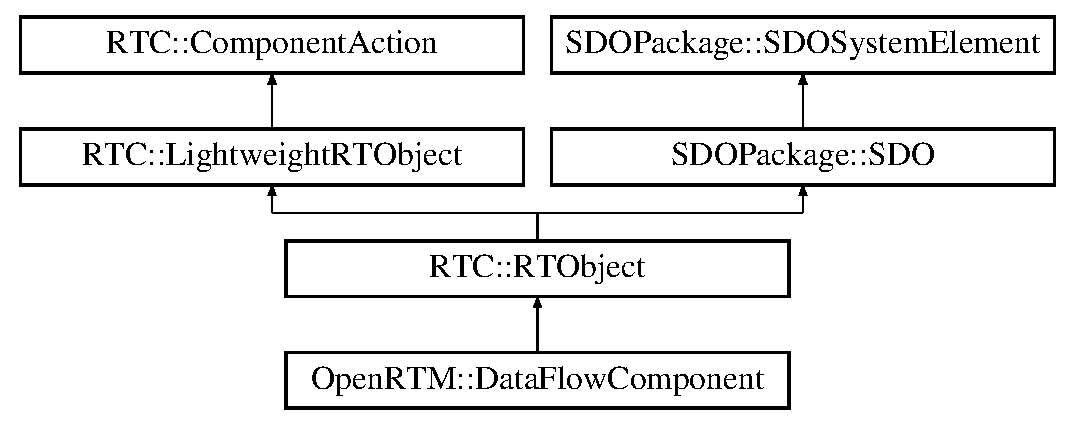
\includegraphics[height=4cm]{interfaceRTC_1_1RTObject}
\end{center}
\end{figure}
\subsection*{Public メソッド}
\begin{DoxyCompactItemize}
\item 
{\bf ComponentProfile} {\bf get\_\-component\_\-profile} ()
\item 
{\bf PortServiceList} {\bf get\_\-ports} ()
\item 
{\bf ReturnCode\_\-t} {\bf initialize} ()
\item 
{\bf ReturnCode\_\-t} {\bf finalize} ()
\item 
boolean {\bf is\_\-alive} (in {\bf ExecutionContext} exec\_\-context)
\item 
{\bf ReturnCode\_\-t} {\bf exit} ()
\item 
{\bf ExecutionContextHandle\_\-t} {\bf attach\_\-context} (in {\bf ExecutionContext} exec\_\-context)
\item 
{\bf ReturnCode\_\-t} {\bf detach\_\-context} (in {\bf ExecutionContextHandle\_\-t} exec\_\-handle)
\item 
{\bf ExecutionContext} {\bf get\_\-context} (in {\bf ExecutionContextHandle\_\-t} exec\_\-handle)
\item 
{\bf ExecutionContextList} {\bf get\_\-owned\_\-contexts} ()
\begin{DoxyCompactList}\small\item\em get\_\-owned\_\-contexts \item\end{DoxyCompactList}\item 
{\bf ExecutionContextList} {\bf get\_\-participating\_\-contexts} ()
\begin{DoxyCompactList}\small\item\em get\_\-participating\_\-contexts \item\end{DoxyCompactList}\item 
{\bf ExecutionContextHandle\_\-t} {\bf get\_\-context\_\-handle} (in {\bf ExecutionContext} cxt)
\item 
{\bf ReturnCode\_\-t} {\bf on\_\-initialize} ()
\item 
{\bf ReturnCode\_\-t} {\bf on\_\-finalize} ()
\item 
{\bf ReturnCode\_\-t} {\bf on\_\-startup} (in {\bf ExecutionContextHandle\_\-t} exec\_\-handle)
\item 
{\bf ReturnCode\_\-t} {\bf on\_\-shutdown} (in {\bf ExecutionContextHandle\_\-t} exec\_\-handle)
\item 
{\bf ReturnCode\_\-t} {\bf on\_\-activated} (in {\bf ExecutionContextHandle\_\-t} exec\_\-handle)
\item 
{\bf ReturnCode\_\-t} {\bf on\_\-deactivated} (in {\bf ExecutionContextHandle\_\-t} exec\_\-handle)
\item 
{\bf ReturnCode\_\-t} {\bf on\_\-aborting} (in {\bf ExecutionContextHandle\_\-t} exec\_\-handle)
\item 
{\bf ReturnCode\_\-t} {\bf on\_\-error} (in {\bf ExecutionContextHandle\_\-t} exec\_\-handle)
\item 
{\bf ReturnCode\_\-t} {\bf on\_\-reset} (in {\bf ExecutionContextHandle\_\-t} exec\_\-handle)
\item 
{\bf UniqueIdentifier} {\bf get\_\-sdo\_\-id} ()  raises (NotAvailable, InternalError)
\item 
string {\bf get\_\-sdo\_\-type} ()  raises (NotAvailable, InternalError)
\item 
DeviceProfile {\bf get\_\-device\_\-profile} ()  raises (NotAvailable, InternalError)
\item 
ServiceProfileList {\bf get\_\-service\_\-profiles} ()  raises (NotAvailable, InternalError)
\item 
ServiceProfile {\bf get\_\-service\_\-profile} (in {\bf UniqueIdentifier} id)  raises (InvalidParameter, NotAvailable, InternalError)
\item 
SDOService {\bf get\_\-sdo\_\-service} (in {\bf UniqueIdentifier} id)  raises (InvalidParameter, NotAvailable, InternalError)
\item 
Configuration {\bf get\_\-configuration} ()  raises (InterfaceNotImplemented, NotAvailable, InternalError)
\item 
Monitoring {\bf get\_\-monitoring} ()  raises (InterfaceNotImplemented, NotAvailable, InternalError)
\item 
OrganizationList {\bf get\_\-organizations} ()  raises (NotAvailable, InternalError)
\item 
{\bf NVList} {\bf get\_\-status\_\-list} ()  raises (NotAvailable, InternalError)
\item 
any {\bf get\_\-status} (in string nme)  raises (InvalidParameter, NotAvailable, InternalError)
\item 
OrganizationList {\bf get\_\-owned\_\-organizations} ()  raises (NotAvailable,InternalError)
\end{DoxyCompactItemize}


\subsection{関数}
\index{RTC::RTObject@{RTC::RTObject}!attach\_\-context@{attach\_\-context}}
\index{attach\_\-context@{attach\_\-context}!RTC::RTObject@{RTC::RTObject}}
\subsubsection[{attach\_\-context}]{\setlength{\rightskip}{0pt plus 5cm}{\bf ExecutionContextHandle\_\-t} RTC::LightweightRTObject::attach\_\-context (in {\bf ExecutionContext} {\em exec\_\-context})\hspace{0.3cm}{\ttfamily  [inherited]}}\label{interfaceRTC_1_1LightweightRTObject_a48dbdbcac3254c29ad01d43a4ee5a00c}
\index{RTC::RTObject@{RTC::RTObject}!detach\_\-context@{detach\_\-context}}
\index{detach\_\-context@{detach\_\-context}!RTC::RTObject@{RTC::RTObject}}
\subsubsection[{detach\_\-context}]{\setlength{\rightskip}{0pt plus 5cm}{\bf ReturnCode\_\-t} RTC::LightweightRTObject::detach\_\-context (in {\bf ExecutionContextHandle\_\-t} {\em exec\_\-handle})\hspace{0.3cm}{\ttfamily  [inherited]}}\label{interfaceRTC_1_1LightweightRTObject_a8eb94420ca08e8f7acaa778ed883b9a4}
\index{RTC::RTObject@{RTC::RTObject}!exit@{exit}}
\index{exit@{exit}!RTC::RTObject@{RTC::RTObject}}
\subsubsection[{exit}]{\setlength{\rightskip}{0pt plus 5cm}{\bf ReturnCode\_\-t} RTC::LightweightRTObject::exit ()\hspace{0.3cm}{\ttfamily  [inherited]}}\label{interfaceRTC_1_1LightweightRTObject_a49bd940b6964fa80d696db15b45c2f87}
\index{RTC::RTObject@{RTC::RTObject}!finalize@{finalize}}
\index{finalize@{finalize}!RTC::RTObject@{RTC::RTObject}}
\subsubsection[{finalize}]{\setlength{\rightskip}{0pt plus 5cm}{\bf ReturnCode\_\-t} RTC::LightweightRTObject::finalize ()\hspace{0.3cm}{\ttfamily  [inherited]}}\label{interfaceRTC_1_1LightweightRTObject_a23466f177b4289662ea035be831426ad}
\index{RTC::RTObject@{RTC::RTObject}!get\_\-component\_\-profile@{get\_\-component\_\-profile}}
\index{get\_\-component\_\-profile@{get\_\-component\_\-profile}!RTC::RTObject@{RTC::RTObject}}
\subsubsection[{get\_\-component\_\-profile}]{\setlength{\rightskip}{0pt plus 5cm}{\bf ComponentProfile} RTC::RTObject::get\_\-component\_\-profile ()}\label{interfaceRTC_1_1RTObject_aa75c245c8e7e0dd19148bbe5cefe4dcc}
\index{RTC::RTObject@{RTC::RTObject}!get\_\-configuration@{get\_\-configuration}}
\index{get\_\-configuration@{get\_\-configuration}!RTC::RTObject@{RTC::RTObject}}
\subsubsection[{get\_\-configuration}]{\setlength{\rightskip}{0pt plus 5cm}Configuration SDOPackage::SDO::get\_\-configuration ()  raises (InterfaceNotImplemented, NotAvailable, InternalError)\hspace{0.3cm}{\ttfamily  [inherited]}}\label{interfaceSDOPackage_1_1SDO_a89b6ff35b88f6212355e439a3a47c60a}
\index{RTC::RTObject@{RTC::RTObject}!get\_\-context@{get\_\-context}}
\index{get\_\-context@{get\_\-context}!RTC::RTObject@{RTC::RTObject}}
\subsubsection[{get\_\-context}]{\setlength{\rightskip}{0pt plus 5cm}{\bf ExecutionContext} RTC::LightweightRTObject::get\_\-context (in {\bf ExecutionContextHandle\_\-t} {\em exec\_\-handle})\hspace{0.3cm}{\ttfamily  [inherited]}}\label{interfaceRTC_1_1LightweightRTObject_a7bb123faf81bcb57542c3a17f10948d6}
\index{RTC::RTObject@{RTC::RTObject}!get\_\-context\_\-handle@{get\_\-context\_\-handle}}
\index{get\_\-context\_\-handle@{get\_\-context\_\-handle}!RTC::RTObject@{RTC::RTObject}}
\subsubsection[{get\_\-context\_\-handle}]{\setlength{\rightskip}{0pt plus 5cm}{\bf ExecutionContextHandle\_\-t} RTC::LightweightRTObject::get\_\-context\_\-handle (in {\bf ExecutionContext} {\em cxt})\hspace{0.3cm}{\ttfamily  [inherited]}}\label{interfaceRTC_1_1LightweightRTObject_af54041744c01d68026aa200276e12f45}
\#\#\# [����] \doxyref{RTC.idl}{p.}{RTC_8idl} �ˤϴޤޤ�Ƥ��ʤ���PIM�ˤϴޤޤ�Ƥ��롣 \#\#\# PIM���������� \index{RTC::RTObject@{RTC::RTObject}!get\_\-device\_\-profile@{get\_\-device\_\-profile}}
\index{get\_\-device\_\-profile@{get\_\-device\_\-profile}!RTC::RTObject@{RTC::RTObject}}
\subsubsection[{get\_\-device\_\-profile}]{\setlength{\rightskip}{0pt plus 5cm}DeviceProfile SDOPackage::SDO::get\_\-device\_\-profile ()  raises (NotAvailable, InternalError)\hspace{0.3cm}{\ttfamily  [inherited]}}\label{interfaceSDOPackage_1_1SDO_af96303b2025ea3e340303365b7ad9f0f}
\index{RTC::RTObject@{RTC::RTObject}!get\_\-monitoring@{get\_\-monitoring}}
\index{get\_\-monitoring@{get\_\-monitoring}!RTC::RTObject@{RTC::RTObject}}
\subsubsection[{get\_\-monitoring}]{\setlength{\rightskip}{0pt plus 5cm}Monitoring SDOPackage::SDO::get\_\-monitoring ()  raises (InterfaceNotImplemented, NotAvailable, InternalError)\hspace{0.3cm}{\ttfamily  [inherited]}}\label{interfaceSDOPackage_1_1SDO_a7db6dded91e964ec26085d1fa8f540c9}
\index{RTC::RTObject@{RTC::RTObject}!get\_\-organizations@{get\_\-organizations}}
\index{get\_\-organizations@{get\_\-organizations}!RTC::RTObject@{RTC::RTObject}}
\subsubsection[{get\_\-organizations}]{\setlength{\rightskip}{0pt plus 5cm}OrganizationList SDOPackage::SDO::get\_\-organizations ()  raises (NotAvailable, InternalError)\hspace{0.3cm}{\ttfamily  [inherited]}}\label{interfaceSDOPackage_1_1SDO_aadb5f8bb6eb2529189d3779940607edd}
\index{RTC::RTObject@{RTC::RTObject}!get\_\-owned\_\-contexts@{get\_\-owned\_\-contexts}}
\index{get\_\-owned\_\-contexts@{get\_\-owned\_\-contexts}!RTC::RTObject@{RTC::RTObject}}
\subsubsection[{get\_\-owned\_\-contexts}]{\setlength{\rightskip}{0pt plus 5cm}{\bf ExecutionContextList} RTC::LightweightRTObject::get\_\-owned\_\-contexts ()\hspace{0.3cm}{\ttfamily  [inherited]}}\label{interfaceRTC_1_1LightweightRTObject_aea9dd2a447cc3ddc55f20aab698da408}


get\_\-owned\_\-contexts 

\subsection{Description}\label{interfaceRTC_1_1LightweightRTObject_Description}
���� \doxyref{RTC}{p.}{namespaceRTC} ����ͭ���� \doxyref{ExecutionContext}{p.}{interfaceRTC_1_1ExecutionContext} �Υꥹ�Ȥ�������롣 \index{RTC::RTObject@{RTC::RTObject}!get\_\-owned\_\-organizations@{get\_\-owned\_\-organizations}}
\index{get\_\-owned\_\-organizations@{get\_\-owned\_\-organizations}!RTC::RTObject@{RTC::RTObject}}
\subsubsection[{get\_\-owned\_\-organizations}]{\setlength{\rightskip}{0pt plus 5cm}OrganizationList SDOPackage::SDOSystemElement::get\_\-owned\_\-organizations ()  raises (NotAvailable,InternalError)\hspace{0.3cm}{\ttfamily  [inherited]}}\label{interfaceSDOPackage_1_1SDOSystemElement_a81238047c5dfa47d2cf3ebce1b78b240}
\index{RTC::RTObject@{RTC::RTObject}!get\_\-participating\_\-contexts@{get\_\-participating\_\-contexts}}
\index{get\_\-participating\_\-contexts@{get\_\-participating\_\-contexts}!RTC::RTObject@{RTC::RTObject}}
\subsubsection[{get\_\-participating\_\-contexts}]{\setlength{\rightskip}{0pt plus 5cm}{\bf ExecutionContextList} RTC::LightweightRTObject::get\_\-participating\_\-contexts ()\hspace{0.3cm}{\ttfamily  [inherited]}}\label{interfaceRTC_1_1LightweightRTObject_af2224880b89275ecf82efad0999b022a}


get\_\-participating\_\-contexts 

\subsection{Description}\label{interfaceRTC_1_1LightweightRTObject_Description}
���� \doxyref{RTC}{p.}{namespaceRTC} �����ä��Ƥ��뤹�٤Ƥ� \doxyref{ExecutionContext}{p.}{interfaceRTC_1_1ExecutionContext} �Υꥹ�Ȥ�������롣\subsection{Semantics}\label{interfaceRTC_1_1LightweightRTObject_Semantics}
���Υꥹ�Ȥ˴ޤޤ��¹ԥ���ƥ����Ȥϡ�attach\_\-context ���Ƥӽ� ����뤴�Ȥˡ��ꥹ�Ȥ��ɲä��졢detach\_\-context ���ƤӽФ���뤴 �Ȥˡ��ꥹ�Ȥ���������롣 \index{RTC::RTObject@{RTC::RTObject}!get\_\-ports@{get\_\-ports}}
\index{get\_\-ports@{get\_\-ports}!RTC::RTObject@{RTC::RTObject}}
\subsubsection[{get\_\-ports}]{\setlength{\rightskip}{0pt plus 5cm}{\bf PortServiceList} RTC::RTObject::get\_\-ports ()}\label{interfaceRTC_1_1RTObject_a4e21edb9c244ed8469cb1fb2de48e158}
\index{RTC::RTObject@{RTC::RTObject}!get\_\-sdo\_\-id@{get\_\-sdo\_\-id}}
\index{get\_\-sdo\_\-id@{get\_\-sdo\_\-id}!RTC::RTObject@{RTC::RTObject}}
\subsubsection[{get\_\-sdo\_\-id}]{\setlength{\rightskip}{0pt plus 5cm}{\bf UniqueIdentifier} SDOPackage::SDO::get\_\-sdo\_\-id ()  raises (NotAvailable, InternalError)\hspace{0.3cm}{\ttfamily  [inherited]}}\label{interfaceSDOPackage_1_1SDO_a08ccbbb1855dff27c598c38ce0c5aab1}
\index{RTC::RTObject@{RTC::RTObject}!get\_\-sdo\_\-service@{get\_\-sdo\_\-service}}
\index{get\_\-sdo\_\-service@{get\_\-sdo\_\-service}!RTC::RTObject@{RTC::RTObject}}
\subsubsection[{get\_\-sdo\_\-service}]{\setlength{\rightskip}{0pt plus 5cm}SDOService SDOPackage::SDO::get\_\-sdo\_\-service (in {\bf UniqueIdentifier} {\em id})  raises (InvalidParameter, NotAvailable, InternalError)\hspace{0.3cm}{\ttfamily  [inherited]}}\label{interfaceSDOPackage_1_1SDO_a7d612d97207fecaf134959b93c6b3e60}
\index{RTC::RTObject@{RTC::RTObject}!get\_\-sdo\_\-type@{get\_\-sdo\_\-type}}
\index{get\_\-sdo\_\-type@{get\_\-sdo\_\-type}!RTC::RTObject@{RTC::RTObject}}
\subsubsection[{get\_\-sdo\_\-type}]{\setlength{\rightskip}{0pt plus 5cm}string SDOPackage::SDO::get\_\-sdo\_\-type ()  raises (NotAvailable, InternalError)\hspace{0.3cm}{\ttfamily  [inherited]}}\label{interfaceSDOPackage_1_1SDO_a2b4141376be89eb90fd4904643476320}
\index{RTC::RTObject@{RTC::RTObject}!get\_\-service\_\-profile@{get\_\-service\_\-profile}}
\index{get\_\-service\_\-profile@{get\_\-service\_\-profile}!RTC::RTObject@{RTC::RTObject}}
\subsubsection[{get\_\-service\_\-profile}]{\setlength{\rightskip}{0pt plus 5cm}ServiceProfile SDOPackage::SDO::get\_\-service\_\-profile (in {\bf UniqueIdentifier} {\em id})  raises (InvalidParameter, NotAvailable, InternalError)\hspace{0.3cm}{\ttfamily  [inherited]}}\label{interfaceSDOPackage_1_1SDO_a5ea1929e10ccc5e8b5896c4b0fbee635}
\index{RTC::RTObject@{RTC::RTObject}!get\_\-service\_\-profiles@{get\_\-service\_\-profiles}}
\index{get\_\-service\_\-profiles@{get\_\-service\_\-profiles}!RTC::RTObject@{RTC::RTObject}}
\subsubsection[{get\_\-service\_\-profiles}]{\setlength{\rightskip}{0pt plus 5cm}ServiceProfileList SDOPackage::SDO::get\_\-service\_\-profiles ()  raises (NotAvailable, InternalError)\hspace{0.3cm}{\ttfamily  [inherited]}}\label{interfaceSDOPackage_1_1SDO_af455c384fa54ab6872d28db1baec3a1d}
\index{RTC::RTObject@{RTC::RTObject}!get\_\-status@{get\_\-status}}
\index{get\_\-status@{get\_\-status}!RTC::RTObject@{RTC::RTObject}}
\subsubsection[{get\_\-status}]{\setlength{\rightskip}{0pt plus 5cm}any SDOPackage::SDO::get\_\-status (in string {\em nme})  raises (InvalidParameter, NotAvailable, InternalError)\hspace{0.3cm}{\ttfamily  [inherited]}}\label{interfaceSDOPackage_1_1SDO_a2655f624a38b590593154c8a8c11e6e8}
\index{RTC::RTObject@{RTC::RTObject}!get\_\-status\_\-list@{get\_\-status\_\-list}}
\index{get\_\-status\_\-list@{get\_\-status\_\-list}!RTC::RTObject@{RTC::RTObject}}
\subsubsection[{get\_\-status\_\-list}]{\setlength{\rightskip}{0pt plus 5cm}{\bf NVList} SDOPackage::SDO::get\_\-status\_\-list ()  raises (NotAvailable, InternalError)\hspace{0.3cm}{\ttfamily  [inherited]}}\label{interfaceSDOPackage_1_1SDO_ae019ba73a5675a871701153bc56db14c}
\index{RTC::RTObject@{RTC::RTObject}!initialize@{initialize}}
\index{initialize@{initialize}!RTC::RTObject@{RTC::RTObject}}
\subsubsection[{initialize}]{\setlength{\rightskip}{0pt plus 5cm}{\bf ReturnCode\_\-t} RTC::LightweightRTObject::initialize ()\hspace{0.3cm}{\ttfamily  [inherited]}}\label{interfaceRTC_1_1LightweightRTObject_afb28c4d97677804da09488578b840eb5}
\index{RTC::RTObject@{RTC::RTObject}!is\_\-alive@{is\_\-alive}}
\index{is\_\-alive@{is\_\-alive}!RTC::RTObject@{RTC::RTObject}}
\subsubsection[{is\_\-alive}]{\setlength{\rightskip}{0pt plus 5cm}boolean RTC::LightweightRTObject::is\_\-alive (in {\bf ExecutionContext} {\em exec\_\-context})\hspace{0.3cm}{\ttfamily  [inherited]}}\label{interfaceRTC_1_1LightweightRTObject_aa07c8c299b0addc49887508c1ee7be27}
\index{RTC::RTObject@{RTC::RTObject}!on\_\-aborting@{on\_\-aborting}}
\index{on\_\-aborting@{on\_\-aborting}!RTC::RTObject@{RTC::RTObject}}
\subsubsection[{on\_\-aborting}]{\setlength{\rightskip}{0pt plus 5cm}{\bf ReturnCode\_\-t} RTC::ComponentAction::on\_\-aborting (in {\bf ExecutionContextHandle\_\-t} {\em exec\_\-handle})\hspace{0.3cm}{\ttfamily  [inherited]}}\label{interfaceRTC_1_1ComponentAction_a876e58ebcea16c307e131b3e6a58ddbe}
\index{RTC::RTObject@{RTC::RTObject}!on\_\-activated@{on\_\-activated}}
\index{on\_\-activated@{on\_\-activated}!RTC::RTObject@{RTC::RTObject}}
\subsubsection[{on\_\-activated}]{\setlength{\rightskip}{0pt plus 5cm}{\bf ReturnCode\_\-t} RTC::ComponentAction::on\_\-activated (in {\bf ExecutionContextHandle\_\-t} {\em exec\_\-handle})\hspace{0.3cm}{\ttfamily  [inherited]}}\label{interfaceRTC_1_1ComponentAction_a4f51f627067d0c54e89c4c0827fa6432}
\index{RTC::RTObject@{RTC::RTObject}!on\_\-deactivated@{on\_\-deactivated}}
\index{on\_\-deactivated@{on\_\-deactivated}!RTC::RTObject@{RTC::RTObject}}
\subsubsection[{on\_\-deactivated}]{\setlength{\rightskip}{0pt plus 5cm}{\bf ReturnCode\_\-t} RTC::ComponentAction::on\_\-deactivated (in {\bf ExecutionContextHandle\_\-t} {\em exec\_\-handle})\hspace{0.3cm}{\ttfamily  [inherited]}}\label{interfaceRTC_1_1ComponentAction_aa5f9cfb9677ba685be333ad666c87f88}
\index{RTC::RTObject@{RTC::RTObject}!on\_\-error@{on\_\-error}}
\index{on\_\-error@{on\_\-error}!RTC::RTObject@{RTC::RTObject}}
\subsubsection[{on\_\-error}]{\setlength{\rightskip}{0pt plus 5cm}{\bf ReturnCode\_\-t} RTC::ComponentAction::on\_\-error (in {\bf ExecutionContextHandle\_\-t} {\em exec\_\-handle})\hspace{0.3cm}{\ttfamily  [inherited]}}\label{interfaceRTC_1_1ComponentAction_a110fdde803e9b13f27308b897439962a}
\index{RTC::RTObject@{RTC::RTObject}!on\_\-finalize@{on\_\-finalize}}
\index{on\_\-finalize@{on\_\-finalize}!RTC::RTObject@{RTC::RTObject}}
\subsubsection[{on\_\-finalize}]{\setlength{\rightskip}{0pt plus 5cm}{\bf ReturnCode\_\-t} RTC::ComponentAction::on\_\-finalize ()\hspace{0.3cm}{\ttfamily  [inherited]}}\label{interfaceRTC_1_1ComponentAction_a9c9e2d638cd2b748609be8a23410aedc}
\index{RTC::RTObject@{RTC::RTObject}!on\_\-initialize@{on\_\-initialize}}
\index{on\_\-initialize@{on\_\-initialize}!RTC::RTObject@{RTC::RTObject}}
\subsubsection[{on\_\-initialize}]{\setlength{\rightskip}{0pt plus 5cm}{\bf ReturnCode\_\-t} RTC::ComponentAction::on\_\-initialize ()\hspace{0.3cm}{\ttfamily  [inherited]}}\label{interfaceRTC_1_1ComponentAction_a8703b183bc1bed9e2fd3ecac126cb231}
\index{RTC::RTObject@{RTC::RTObject}!on\_\-reset@{on\_\-reset}}
\index{on\_\-reset@{on\_\-reset}!RTC::RTObject@{RTC::RTObject}}
\subsubsection[{on\_\-reset}]{\setlength{\rightskip}{0pt plus 5cm}{\bf ReturnCode\_\-t} RTC::ComponentAction::on\_\-reset (in {\bf ExecutionContextHandle\_\-t} {\em exec\_\-handle})\hspace{0.3cm}{\ttfamily  [inherited]}}\label{interfaceRTC_1_1ComponentAction_adb0e61bff251337d79c7c7d050d8304e}
\index{RTC::RTObject@{RTC::RTObject}!on\_\-shutdown@{on\_\-shutdown}}
\index{on\_\-shutdown@{on\_\-shutdown}!RTC::RTObject@{RTC::RTObject}}
\subsubsection[{on\_\-shutdown}]{\setlength{\rightskip}{0pt plus 5cm}{\bf ReturnCode\_\-t} RTC::ComponentAction::on\_\-shutdown (in {\bf ExecutionContextHandle\_\-t} {\em exec\_\-handle})\hspace{0.3cm}{\ttfamily  [inherited]}}\label{interfaceRTC_1_1ComponentAction_accc47711344c811c9bdba0d66a3048f2}
\index{RTC::RTObject@{RTC::RTObject}!on\_\-startup@{on\_\-startup}}
\index{on\_\-startup@{on\_\-startup}!RTC::RTObject@{RTC::RTObject}}
\subsubsection[{on\_\-startup}]{\setlength{\rightskip}{0pt plus 5cm}{\bf ReturnCode\_\-t} RTC::ComponentAction::on\_\-startup (in {\bf ExecutionContextHandle\_\-t} {\em exec\_\-handle})\hspace{0.3cm}{\ttfamily  [inherited]}}\label{interfaceRTC_1_1ComponentAction_ac305f00c92f4650cf4fc798aac37eef2}


このインタフェースの説明は次のファイルから生成されました:\begin{DoxyCompactItemize}
\item 
{\bf RTC.idl}\end{DoxyCompactItemize}

\section{SDOPackage::SDO Interface Reference}
\label{interfaceSDOPackage_1_1SDO}\index{SDOPackage::SDO@{SDOPackage::SDO}}


{\ttfamily import \char`\"{}SDOPackage.idl\char`\"{};}

Inheritance diagram for SDOPackage::SDO:\begin{figure}[H]
\begin{center}
\leavevmode
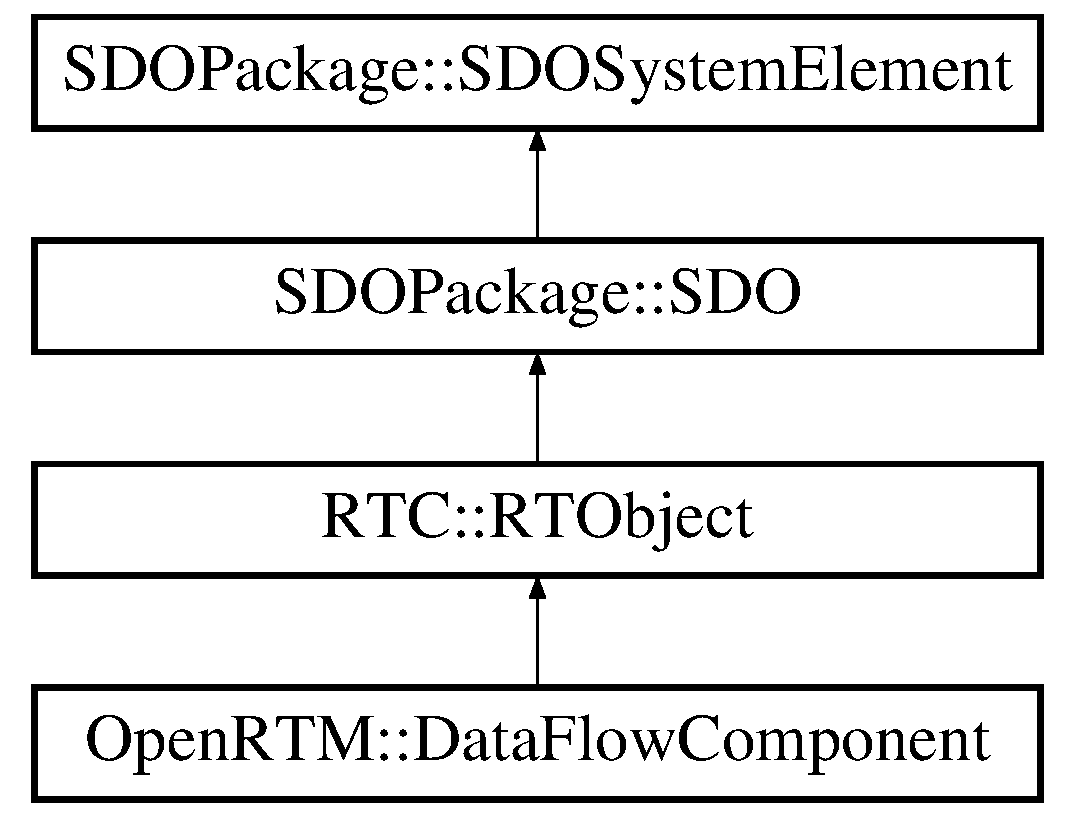
\includegraphics[height=4cm]{interfaceSDOPackage_1_1SDO}
\end{center}
\end{figure}
\subsection*{Public Member Functions}
\begin{DoxyCompactItemize}
\item 
{\bf UniqueIdentifier} {\bf get\_\-sdo\_\-id} ()  raises (NotAvailable, InternalError)
\item 
string {\bf get\_\-sdo\_\-type} ()  raises (NotAvailable, InternalError)
\item 
{\bf DeviceProfile} {\bf get\_\-device\_\-profile} ()  raises (NotAvailable, InternalError)
\item 
{\bf ServiceProfileList} {\bf get\_\-service\_\-profiles} ()  raises (NotAvailable, InternalError)
\item 
{\bf ServiceProfile} {\bf get\_\-service\_\-profile} (in {\bf UniqueIdentifier} id)  raises (InvalidParameter, NotAvailable, InternalError)
\item 
{\bf SDOService} {\bf get\_\-sdo\_\-service} (in {\bf UniqueIdentifier} id)  raises (InvalidParameter, NotAvailable, InternalError)
\item 
{\bf Configuration} {\bf get\_\-configuration} ()  raises (InterfaceNotImplemented, NotAvailable, InternalError)
\item 
{\bf Monitoring} {\bf get\_\-monitoring} ()  raises (InterfaceNotImplemented, NotAvailable, InternalError)
\item 
{\bf OrganizationList} {\bf get\_\-organizations} ()  raises (NotAvailable, InternalError)
\item 
{\bf NVList} {\bf get\_\-status\_\-list} ()  raises (NotAvailable, InternalError)
\item 
any {\bf get\_\-status} (in string nme)  raises (InvalidParameter, NotAvailable, InternalError)
\item 
{\bf OrganizationList} {\bf get\_\-owned\_\-organizations} ()  raises (NotAvailable,InternalError)
\end{DoxyCompactItemize}


\subsection{Member Function Documentation}
\index{SDOPackage::SDO@{SDOPackage::SDO}!get\_\-configuration@{get\_\-configuration}}
\index{get\_\-configuration@{get\_\-configuration}!SDOPackage::SDO@{SDOPackage::SDO}}
\subsubsection[{get\_\-configuration}]{\setlength{\rightskip}{0pt plus 5cm}{\bf Configuration} SDOPackage::SDO::get\_\-configuration ()  raises (InterfaceNotImplemented, NotAvailable, InternalError)}\label{interfaceSDOPackage_1_1SDO_a89b6ff35b88f6212355e439a3a47c60a}
\index{SDOPackage::SDO@{SDOPackage::SDO}!get\_\-device\_\-profile@{get\_\-device\_\-profile}}
\index{get\_\-device\_\-profile@{get\_\-device\_\-profile}!SDOPackage::SDO@{SDOPackage::SDO}}
\subsubsection[{get\_\-device\_\-profile}]{\setlength{\rightskip}{0pt plus 5cm}{\bf DeviceProfile} SDOPackage::SDO::get\_\-device\_\-profile ()  raises (NotAvailable, InternalError)}\label{interfaceSDOPackage_1_1SDO_af96303b2025ea3e340303365b7ad9f0f}
\index{SDOPackage::SDO@{SDOPackage::SDO}!get\_\-monitoring@{get\_\-monitoring}}
\index{get\_\-monitoring@{get\_\-monitoring}!SDOPackage::SDO@{SDOPackage::SDO}}
\subsubsection[{get\_\-monitoring}]{\setlength{\rightskip}{0pt plus 5cm}{\bf Monitoring} SDOPackage::SDO::get\_\-monitoring ()  raises (InterfaceNotImplemented, NotAvailable, InternalError)}\label{interfaceSDOPackage_1_1SDO_a7db6dded91e964ec26085d1fa8f540c9}
\index{SDOPackage::SDO@{SDOPackage::SDO}!get\_\-organizations@{get\_\-organizations}}
\index{get\_\-organizations@{get\_\-organizations}!SDOPackage::SDO@{SDOPackage::SDO}}
\subsubsection[{get\_\-organizations}]{\setlength{\rightskip}{0pt plus 5cm}{\bf OrganizationList} SDOPackage::SDO::get\_\-organizations ()  raises (NotAvailable, InternalError)}\label{interfaceSDOPackage_1_1SDO_aadb5f8bb6eb2529189d3779940607edd}
\index{SDOPackage::SDO@{SDOPackage::SDO}!get\_\-owned\_\-organizations@{get\_\-owned\_\-organizations}}
\index{get\_\-owned\_\-organizations@{get\_\-owned\_\-organizations}!SDOPackage::SDO@{SDOPackage::SDO}}
\subsubsection[{get\_\-owned\_\-organizations}]{\setlength{\rightskip}{0pt plus 5cm}{\bf OrganizationList} SDOPackage::SDOSystemElement::get\_\-owned\_\-organizations ()  raises (NotAvailable,InternalError)\hspace{0.3cm}{\ttfamily  [inherited]}}\label{interfaceSDOPackage_1_1SDOSystemElement_a81238047c5dfa47d2cf3ebce1b78b240}
\index{SDOPackage::SDO@{SDOPackage::SDO}!get\_\-sdo\_\-id@{get\_\-sdo\_\-id}}
\index{get\_\-sdo\_\-id@{get\_\-sdo\_\-id}!SDOPackage::SDO@{SDOPackage::SDO}}
\subsubsection[{get\_\-sdo\_\-id}]{\setlength{\rightskip}{0pt plus 5cm}{\bf UniqueIdentifier} SDOPackage::SDO::get\_\-sdo\_\-id ()  raises (NotAvailable, InternalError)}\label{interfaceSDOPackage_1_1SDO_a08ccbbb1855dff27c598c38ce0c5aab1}
\index{SDOPackage::SDO@{SDOPackage::SDO}!get\_\-sdo\_\-service@{get\_\-sdo\_\-service}}
\index{get\_\-sdo\_\-service@{get\_\-sdo\_\-service}!SDOPackage::SDO@{SDOPackage::SDO}}
\subsubsection[{get\_\-sdo\_\-service}]{\setlength{\rightskip}{0pt plus 5cm}{\bf SDOService} SDOPackage::SDO::get\_\-sdo\_\-service (in {\bf UniqueIdentifier} {\em id})  raises (InvalidParameter, NotAvailable, InternalError)}\label{interfaceSDOPackage_1_1SDO_a7d612d97207fecaf134959b93c6b3e60}
\index{SDOPackage::SDO@{SDOPackage::SDO}!get\_\-sdo\_\-type@{get\_\-sdo\_\-type}}
\index{get\_\-sdo\_\-type@{get\_\-sdo\_\-type}!SDOPackage::SDO@{SDOPackage::SDO}}
\subsubsection[{get\_\-sdo\_\-type}]{\setlength{\rightskip}{0pt plus 5cm}string SDOPackage::SDO::get\_\-sdo\_\-type ()  raises (NotAvailable, InternalError)}\label{interfaceSDOPackage_1_1SDO_a2b4141376be89eb90fd4904643476320}
\index{SDOPackage::SDO@{SDOPackage::SDO}!get\_\-service\_\-profile@{get\_\-service\_\-profile}}
\index{get\_\-service\_\-profile@{get\_\-service\_\-profile}!SDOPackage::SDO@{SDOPackage::SDO}}
\subsubsection[{get\_\-service\_\-profile}]{\setlength{\rightskip}{0pt plus 5cm}{\bf ServiceProfile} SDOPackage::SDO::get\_\-service\_\-profile (in {\bf UniqueIdentifier} {\em id})  raises (InvalidParameter, NotAvailable, InternalError)}\label{interfaceSDOPackage_1_1SDO_a5ea1929e10ccc5e8b5896c4b0fbee635}
\index{SDOPackage::SDO@{SDOPackage::SDO}!get\_\-service\_\-profiles@{get\_\-service\_\-profiles}}
\index{get\_\-service\_\-profiles@{get\_\-service\_\-profiles}!SDOPackage::SDO@{SDOPackage::SDO}}
\subsubsection[{get\_\-service\_\-profiles}]{\setlength{\rightskip}{0pt plus 5cm}{\bf ServiceProfileList} SDOPackage::SDO::get\_\-service\_\-profiles ()  raises (NotAvailable, InternalError)}\label{interfaceSDOPackage_1_1SDO_af455c384fa54ab6872d28db1baec3a1d}
\index{SDOPackage::SDO@{SDOPackage::SDO}!get\_\-status@{get\_\-status}}
\index{get\_\-status@{get\_\-status}!SDOPackage::SDO@{SDOPackage::SDO}}
\subsubsection[{get\_\-status}]{\setlength{\rightskip}{0pt plus 5cm}any SDOPackage::SDO::get\_\-status (in string {\em nme})  raises (InvalidParameter, NotAvailable, InternalError)}\label{interfaceSDOPackage_1_1SDO_a2655f624a38b590593154c8a8c11e6e8}
\index{SDOPackage::SDO@{SDOPackage::SDO}!get\_\-status\_\-list@{get\_\-status\_\-list}}
\index{get\_\-status\_\-list@{get\_\-status\_\-list}!SDOPackage::SDO@{SDOPackage::SDO}}
\subsubsection[{get\_\-status\_\-list}]{\setlength{\rightskip}{0pt plus 5cm}{\bf NVList} SDOPackage::SDO::get\_\-status\_\-list ()  raises (NotAvailable, InternalError)}\label{interfaceSDOPackage_1_1SDO_ae019ba73a5675a871701153bc56db14c}


The documentation for this interface was generated from the following file:\begin{DoxyCompactItemize}
\item 
{\bf SDOPackage.idl}\end{DoxyCompactItemize}

\section{インタフェース SDOPackage::SDOService}
\label{interfaceSDOPackage_1_1SDOService}\index{SDOPackage::SDOService@{SDOPackage::SDOService}}


{\ttfamily import \char`\"{}SDOPackage.idl\char`\"{};}

SDOPackage::SDOServiceに対する継承グラフ\begin{figure}[H]
\begin{center}
\leavevmode
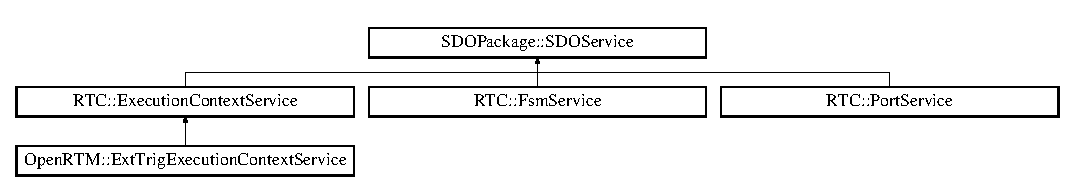
\includegraphics[height=2.12928cm]{interfaceSDOPackage_1_1SDOService}
\end{center}
\end{figure}


このインタフェースの説明は次のファイルから生成されました:\begin{DoxyCompactItemize}
\item 
{\bf SDOPackage.idl}\end{DoxyCompactItemize}

\section{SDOPackage::SDOSystemElement Interface Reference}
\label{interfaceSDOPackage_1_1SDOSystemElement}\index{SDOPackage::SDOSystemElement@{SDOPackage::SDOSystemElement}}


{\ttfamily import \char`\"{}SDOPackage.idl\char`\"{};}

Inheritance diagram for SDOPackage::SDOSystemElement:\begin{figure}[H]
\begin{center}
\leavevmode
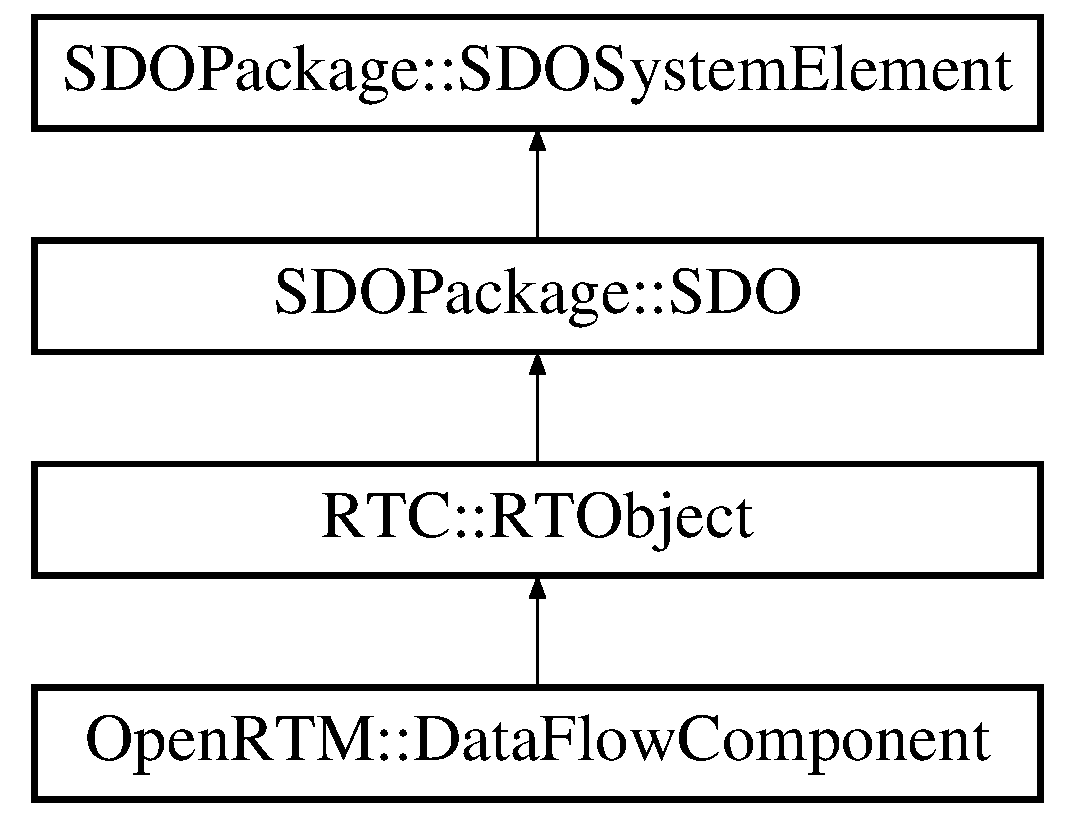
\includegraphics[height=4cm]{interfaceSDOPackage_1_1SDOSystemElement}
\end{center}
\end{figure}
\subsection*{Public Member Functions}
\begin{DoxyCompactItemize}
\item 
{\bf OrganizationList} {\bf get\_\-owned\_\-organizations} ()  raises (NotAvailable,InternalError)
\end{DoxyCompactItemize}


\subsection{Detailed Description}
-\/-\/-\/-\/-\/-\/-\/ Interfaces -\/-\/-\/-\/-\/-\/-\/ 

\subsection{Member Function Documentation}
\index{SDOPackage::SDOSystemElement@{SDOPackage::SDOSystemElement}!get\_\-owned\_\-organizations@{get\_\-owned\_\-organizations}}
\index{get\_\-owned\_\-organizations@{get\_\-owned\_\-organizations}!SDOPackage::SDOSystemElement@{SDOPackage::SDOSystemElement}}
\subsubsection[{get\_\-owned\_\-organizations}]{\setlength{\rightskip}{0pt plus 5cm}{\bf OrganizationList} SDOPackage::SDOSystemElement::get\_\-owned\_\-organizations ()  raises (NotAvailable,InternalError)}\label{interfaceSDOPackage_1_1SDOSystemElement_a81238047c5dfa47d2cf3ebce1b78b240}


The documentation for this interface was generated from the following file:\begin{DoxyCompactItemize}
\item 
{\bf SDOPackage.idl}\end{DoxyCompactItemize}

\section{SDOPackage::ServiceProfile Struct Reference}
\label{structSDOPackage_1_1ServiceProfile}\index{SDOPackage::ServiceProfile@{SDOPackage::ServiceProfile}}


{\ttfamily import \char`\"{}SDOPackage.idl\char`\"{};}

\subsection*{Public Attributes}
\begin{DoxyCompactItemize}
\item 
string {\bf id}
\item 
string {\bf interface\_\-type}
\item 
{\bf NVList} {\bf properties}
\item 
{\bf SDOService} {\bf service}
\end{DoxyCompactItemize}


\subsection{Member Data Documentation}
\index{SDOPackage::ServiceProfile@{SDOPackage::ServiceProfile}!id@{id}}
\index{id@{id}!SDOPackage::ServiceProfile@{SDOPackage::ServiceProfile}}
\subsubsection[{id}]{\setlength{\rightskip}{0pt plus 5cm}string {\bf SDOPackage::ServiceProfile::id}}\label{structSDOPackage_1_1ServiceProfile_a147cc3a82086729b503a8838fb87207d}
\index{SDOPackage::ServiceProfile@{SDOPackage::ServiceProfile}!interface\_\-type@{interface\_\-type}}
\index{interface\_\-type@{interface\_\-type}!SDOPackage::ServiceProfile@{SDOPackage::ServiceProfile}}
\subsubsection[{interface\_\-type}]{\setlength{\rightskip}{0pt plus 5cm}string {\bf SDOPackage::ServiceProfile::interface\_\-type}}\label{structSDOPackage_1_1ServiceProfile_a3cca8b894a7ca01c338bd892d3b43e59}
\index{SDOPackage::ServiceProfile@{SDOPackage::ServiceProfile}!properties@{properties}}
\index{properties@{properties}!SDOPackage::ServiceProfile@{SDOPackage::ServiceProfile}}
\subsubsection[{properties}]{\setlength{\rightskip}{0pt plus 5cm}{\bf NVList} {\bf SDOPackage::ServiceProfile::properties}}\label{structSDOPackage_1_1ServiceProfile_aef2aa811254bff3cc038c377cf23562d}
\index{SDOPackage::ServiceProfile@{SDOPackage::ServiceProfile}!service@{service}}
\index{service@{service}!SDOPackage::ServiceProfile@{SDOPackage::ServiceProfile}}
\subsubsection[{service}]{\setlength{\rightskip}{0pt plus 5cm}{\bf SDOService} {\bf SDOPackage::ServiceProfile::service}}\label{structSDOPackage_1_1ServiceProfile_a603c6ea80a4a86c0dc1dad9f20d96efb}


The documentation for this struct was generated from the following file:\begin{DoxyCompactItemize}
\item 
{\bf SDOPackage.idl}\end{DoxyCompactItemize}

\section{RTC::Time Struct Reference}
\label{structRTC_1_1Time}\index{RTC::Time@{RTC::Time}}


{\ttfamily import \char`\"{}BasicDataType.idl\char`\"{};}

\subsection*{Public Attributes}
\begin{DoxyCompactItemize}
\item 
unsigned long {\bf sec}
\item 
unsigned long {\bf nsec}
\end{DoxyCompactItemize}


\subsection{Member Data Documentation}
\index{RTC::Time@{RTC::Time}!nsec@{nsec}}
\index{nsec@{nsec}!RTC::Time@{RTC::Time}}
\subsubsection[{nsec}]{\setlength{\rightskip}{0pt plus 5cm}unsigned long {\bf RTC::Time::nsec}}\label{structRTC_1_1Time_af90fdb43cc4cd394cc9e097e673821be}
\index{RTC::Time@{RTC::Time}!sec@{sec}}
\index{sec@{sec}!RTC::Time@{RTC::Time}}
\subsubsection[{sec}]{\setlength{\rightskip}{0pt plus 5cm}unsigned long {\bf RTC::Time::sec}}\label{structRTC_1_1Time_a1ed073c8e58d7465a571f839514d53a5}


The documentation for this struct was generated from the following file:\begin{DoxyCompactItemize}
\item 
{\bf BasicDataType.idl}\end{DoxyCompactItemize}

\section{RTC::TimedBoolean Struct Reference}
\label{structRTC_1_1TimedBoolean}\index{RTC::TimedBoolean@{RTC::TimedBoolean}}


{\ttfamily import \char`\"{}BasicDataType.idl\char`\"{};}

\subsection*{Public Attributes}
\begin{DoxyCompactItemize}
\item 
{\bf Time} {\bf tm}
\item 
boolean {\bf data}
\end{DoxyCompactItemize}


\subsection{Member Data Documentation}
\index{RTC::TimedBoolean@{RTC::TimedBoolean}!data@{data}}
\index{data@{data}!RTC::TimedBoolean@{RTC::TimedBoolean}}
\subsubsection[{data}]{\setlength{\rightskip}{0pt plus 5cm}boolean {\bf RTC::TimedBoolean::data}}\label{structRTC_1_1TimedBoolean_a13a5e2dcf6f1f84895268e835a1a504c}
\index{RTC::TimedBoolean@{RTC::TimedBoolean}!tm@{tm}}
\index{tm@{tm}!RTC::TimedBoolean@{RTC::TimedBoolean}}
\subsubsection[{tm}]{\setlength{\rightskip}{0pt plus 5cm}{\bf Time} {\bf RTC::TimedBoolean::tm}}\label{structRTC_1_1TimedBoolean_aa07e1f41460e4542fe94af48e0e0135e}


The documentation for this struct was generated from the following file:\begin{DoxyCompactItemize}
\item 
{\bf BasicDataType.idl}\end{DoxyCompactItemize}

\section{構造体 RTC::TimedBooleanSeq}
\label{structRTC_1_1TimedBooleanSeq}\index{RTC::TimedBooleanSeq@{RTC::TimedBooleanSeq}}


{\ttfamily import \char`\"{}BasicDataType.idl\char`\"{};}

\subsection*{Public 変数}
\begin{DoxyCompactItemize}
\item 
{\bf Time} {\bf tm}
\item 
sequence$<$ boolean $>$ {\bf data}
\end{DoxyCompactItemize}


\subsection{変数}
\index{RTC::TimedBooleanSeq@{RTC::TimedBooleanSeq}!data@{data}}
\index{data@{data}!RTC::TimedBooleanSeq@{RTC::TimedBooleanSeq}}
\subsubsection[{data}]{\setlength{\rightskip}{0pt plus 5cm}sequence$<$boolean$>$ {\bf RTC::TimedBooleanSeq::data}}\label{structRTC_1_1TimedBooleanSeq_aae5d5a31e52ad9059ecc9eb7d9db8f01}
\index{RTC::TimedBooleanSeq@{RTC::TimedBooleanSeq}!tm@{tm}}
\index{tm@{tm}!RTC::TimedBooleanSeq@{RTC::TimedBooleanSeq}}
\subsubsection[{tm}]{\setlength{\rightskip}{0pt plus 5cm}{\bf Time} {\bf RTC::TimedBooleanSeq::tm}}\label{structRTC_1_1TimedBooleanSeq_a79569ec043f6684c520ec5abf81d1933}


この構造体の説明は次のファイルから生成されました:\begin{DoxyCompactItemize}
\item 
{\bf BasicDataType.idl}\end{DoxyCompactItemize}

\section{構造体 RTC::TimedChar}
\label{structRTC_1_1TimedChar}\index{RTC::TimedChar@{RTC::TimedChar}}


{\ttfamily import \char`\"{}BasicDataType.idl\char`\"{};}

\subsection*{Public 変数}
\begin{DoxyCompactItemize}
\item 
{\bf Time} {\bf tm}
\item 
char {\bf data}
\end{DoxyCompactItemize}


\subsection{変数}
\index{RTC::TimedChar@{RTC::TimedChar}!data@{data}}
\index{data@{data}!RTC::TimedChar@{RTC::TimedChar}}
\subsubsection[{data}]{\setlength{\rightskip}{0pt plus 5cm}char {\bf RTC::TimedChar::data}}\label{structRTC_1_1TimedChar_a448dbbc6aa602a9314da5ce19a49dd59}
\index{RTC::TimedChar@{RTC::TimedChar}!tm@{tm}}
\index{tm@{tm}!RTC::TimedChar@{RTC::TimedChar}}
\subsubsection[{tm}]{\setlength{\rightskip}{0pt plus 5cm}{\bf Time} {\bf RTC::TimedChar::tm}}\label{structRTC_1_1TimedChar_a7c25b6d06dc64102f94a400d6a5b4e0e}


この構造体の説明は次のファイルから生成されました:\begin{DoxyCompactItemize}
\item 
{\bf BasicDataType.idl}\end{DoxyCompactItemize}

\section{RTC::TimedCharSeq Struct Reference}
\label{structRTC_1_1TimedCharSeq}\index{RTC::TimedCharSeq@{RTC::TimedCharSeq}}


{\ttfamily import \char`\"{}BasicDataType.idl\char`\"{};}

\subsection*{Public Attributes}
\begin{DoxyCompactItemize}
\item 
{\bf Time} {\bf tm}
\item 
sequence$<$ char $>$ {\bf data}
\end{DoxyCompactItemize}


\subsection{Member Data Documentation}
\index{RTC::TimedCharSeq@{RTC::TimedCharSeq}!data@{data}}
\index{data@{data}!RTC::TimedCharSeq@{RTC::TimedCharSeq}}
\subsubsection[{data}]{\setlength{\rightskip}{0pt plus 5cm}sequence$<$char$>$ {\bf RTC::TimedCharSeq::data}}\label{structRTC_1_1TimedCharSeq_a56ac1b4edf9feed206c4f5dac3f39a76}
\index{RTC::TimedCharSeq@{RTC::TimedCharSeq}!tm@{tm}}
\index{tm@{tm}!RTC::TimedCharSeq@{RTC::TimedCharSeq}}
\subsubsection[{tm}]{\setlength{\rightskip}{0pt plus 5cm}{\bf Time} {\bf RTC::TimedCharSeq::tm}}\label{structRTC_1_1TimedCharSeq_adf1cef916575772777ad789c69311a2c}


The documentation for this struct was generated from the following file:\begin{DoxyCompactItemize}
\item 
{\bf BasicDataType.idl}\end{DoxyCompactItemize}

\section{構造体 RTC::TimedDouble}
\label{structRTC_1_1TimedDouble}\index{RTC::TimedDouble@{RTC::TimedDouble}}


{\ttfamily import \char`\"{}BasicDataType.idl\char`\"{};}

\subsection*{Public 変数}
\begin{DoxyCompactItemize}
\item 
{\bf Time} {\bf tm}
\item 
double {\bf data}
\end{DoxyCompactItemize}


\subsection{変数}
\index{RTC::TimedDouble@{RTC::TimedDouble}!data@{data}}
\index{data@{data}!RTC::TimedDouble@{RTC::TimedDouble}}
\subsubsection[{data}]{\setlength{\rightskip}{0pt plus 5cm}double {\bf RTC::TimedDouble::data}}\label{structRTC_1_1TimedDouble_acd572c69d2c9ccbf144ea4d3873056d4}
\index{RTC::TimedDouble@{RTC::TimedDouble}!tm@{tm}}
\index{tm@{tm}!RTC::TimedDouble@{RTC::TimedDouble}}
\subsubsection[{tm}]{\setlength{\rightskip}{0pt plus 5cm}{\bf Time} {\bf RTC::TimedDouble::tm}}\label{structRTC_1_1TimedDouble_a4bf2f8c22004f0180be307ecda4413e2}


この構造体の説明は次のファイルから生成されました:\begin{DoxyCompactItemize}
\item 
{\bf BasicDataType.idl}\end{DoxyCompactItemize}

\section{RTC::TimedDoubleSeq Struct Reference}
\label{structRTC_1_1TimedDoubleSeq}\index{RTC::TimedDoubleSeq@{RTC::TimedDoubleSeq}}


{\ttfamily import \char`\"{}BasicDataType.idl\char`\"{};}

\subsection*{Public Attributes}
\begin{DoxyCompactItemize}
\item 
{\bf Time} {\bf tm}
\item 
sequence$<$ double $>$ {\bf data}
\end{DoxyCompactItemize}


\subsection{Member Data Documentation}
\index{RTC::TimedDoubleSeq@{RTC::TimedDoubleSeq}!data@{data}}
\index{data@{data}!RTC::TimedDoubleSeq@{RTC::TimedDoubleSeq}}
\subsubsection[{data}]{\setlength{\rightskip}{0pt plus 5cm}sequence$<$double$>$ {\bf RTC::TimedDoubleSeq::data}}\label{structRTC_1_1TimedDoubleSeq_ac1f55e29d8e54d08da33d6d81c6309fc}
\index{RTC::TimedDoubleSeq@{RTC::TimedDoubleSeq}!tm@{tm}}
\index{tm@{tm}!RTC::TimedDoubleSeq@{RTC::TimedDoubleSeq}}
\subsubsection[{tm}]{\setlength{\rightskip}{0pt plus 5cm}{\bf Time} {\bf RTC::TimedDoubleSeq::tm}}\label{structRTC_1_1TimedDoubleSeq_aa157419b7a22afc914c73e6958003925}


The documentation for this struct was generated from the following file:\begin{DoxyCompactItemize}
\item 
{\bf BasicDataType.idl}\end{DoxyCompactItemize}

\section{RTC::TimedFloat Struct Reference}
\label{structRTC_1_1TimedFloat}\index{RTC::TimedFloat@{RTC::TimedFloat}}


{\ttfamily import \char`\"{}BasicDataType.idl\char`\"{};}

\subsection*{Public Attributes}
\begin{DoxyCompactItemize}
\item 
{\bf Time} {\bf tm}
\item 
float {\bf data}
\end{DoxyCompactItemize}


\subsection{Member Data Documentation}
\index{RTC::TimedFloat@{RTC::TimedFloat}!data@{data}}
\index{data@{data}!RTC::TimedFloat@{RTC::TimedFloat}}
\subsubsection[{data}]{\setlength{\rightskip}{0pt plus 5cm}float {\bf RTC::TimedFloat::data}}\label{structRTC_1_1TimedFloat_ac071c97d322eda23f48c0f60d33fce28}
\index{RTC::TimedFloat@{RTC::TimedFloat}!tm@{tm}}
\index{tm@{tm}!RTC::TimedFloat@{RTC::TimedFloat}}
\subsubsection[{tm}]{\setlength{\rightskip}{0pt plus 5cm}{\bf Time} {\bf RTC::TimedFloat::tm}}\label{structRTC_1_1TimedFloat_afc52cd219182bd89ac8e76515db1aaea}


The documentation for this struct was generated from the following file:\begin{DoxyCompactItemize}
\item 
{\bf BasicDataType.idl}\end{DoxyCompactItemize}

\section{構造体 RTC::TimedFloatSeq}
\label{structRTC_1_1TimedFloatSeq}\index{RTC::TimedFloatSeq@{RTC::TimedFloatSeq}}


{\ttfamily import \char`\"{}BasicDataType.idl\char`\"{};}

\subsection*{Public 変数}
\begin{DoxyCompactItemize}
\item 
{\bf Time} {\bf tm}
\item 
sequence$<$ float $>$ {\bf data}
\end{DoxyCompactItemize}


\subsection{変数}
\index{RTC::TimedFloatSeq@{RTC::TimedFloatSeq}!data@{data}}
\index{data@{data}!RTC::TimedFloatSeq@{RTC::TimedFloatSeq}}
\subsubsection[{data}]{\setlength{\rightskip}{0pt plus 5cm}sequence$<$float$>$ {\bf RTC::TimedFloatSeq::data}}\label{structRTC_1_1TimedFloatSeq_a797fd0ae3021d0cc9eaccdc2f12b3ad4}
\index{RTC::TimedFloatSeq@{RTC::TimedFloatSeq}!tm@{tm}}
\index{tm@{tm}!RTC::TimedFloatSeq@{RTC::TimedFloatSeq}}
\subsubsection[{tm}]{\setlength{\rightskip}{0pt plus 5cm}{\bf Time} {\bf RTC::TimedFloatSeq::tm}}\label{structRTC_1_1TimedFloatSeq_a9edda8052def84ee7da46c49c9c0bf69}


この構造体の説明は次のファイルから生成されました:\begin{DoxyCompactItemize}
\item 
{\bf BasicDataType.idl}\end{DoxyCompactItemize}

\section{構造体 RTC::TimedLong}
\label{structRTC_1_1TimedLong}\index{RTC::TimedLong@{RTC::TimedLong}}


{\ttfamily import \char`\"{}BasicDataType.idl\char`\"{};}

\subsection*{Public 変数}
\begin{DoxyCompactItemize}
\item 
{\bf Time} {\bf tm}
\item 
long {\bf data}
\end{DoxyCompactItemize}


\subsection{変数}
\index{RTC::TimedLong@{RTC::TimedLong}!data@{data}}
\index{data@{data}!RTC::TimedLong@{RTC::TimedLong}}
\subsubsection[{data}]{\setlength{\rightskip}{0pt plus 5cm}long {\bf RTC::TimedLong::data}}\label{structRTC_1_1TimedLong_a776b78537c9dad5557a57a88a66b5942}
\index{RTC::TimedLong@{RTC::TimedLong}!tm@{tm}}
\index{tm@{tm}!RTC::TimedLong@{RTC::TimedLong}}
\subsubsection[{tm}]{\setlength{\rightskip}{0pt plus 5cm}{\bf Time} {\bf RTC::TimedLong::tm}}\label{structRTC_1_1TimedLong_a9bba771ba1996f1a2e85de1ce77041b9}


この構造体の説明は次のファイルから生成されました:\begin{DoxyCompactItemize}
\item 
{\bf BasicDataType.idl}\end{DoxyCompactItemize}

\section{構造体 RTC::TimedLongSeq}
\label{structRTC_1_1TimedLongSeq}\index{RTC::TimedLongSeq@{RTC::TimedLongSeq}}


{\ttfamily import \char`\"{}BasicDataType.idl\char`\"{};}

\subsection*{Public 変数}
\begin{DoxyCompactItemize}
\item 
{\bf Time} {\bf tm}
\item 
sequence$<$ long $>$ {\bf data}
\end{DoxyCompactItemize}


\subsection{変数}
\index{RTC::TimedLongSeq@{RTC::TimedLongSeq}!data@{data}}
\index{data@{data}!RTC::TimedLongSeq@{RTC::TimedLongSeq}}
\subsubsection[{data}]{\setlength{\rightskip}{0pt plus 5cm}sequence$<$long$>$ {\bf RTC::TimedLongSeq::data}}\label{structRTC_1_1TimedLongSeq_a7cb12c9383805cd91d11667feec996a6}
\index{RTC::TimedLongSeq@{RTC::TimedLongSeq}!tm@{tm}}
\index{tm@{tm}!RTC::TimedLongSeq@{RTC::TimedLongSeq}}
\subsubsection[{tm}]{\setlength{\rightskip}{0pt plus 5cm}{\bf Time} {\bf RTC::TimedLongSeq::tm}}\label{structRTC_1_1TimedLongSeq_ad3b53881eff39c36d3d7718190bf3485}


この構造体の説明は次のファイルから生成されました:\begin{DoxyCompactItemize}
\item 
{\bf BasicDataType.idl}\end{DoxyCompactItemize}

\section{構造体 RTC::TimedOctet}
\label{structRTC_1_1TimedOctet}\index{RTC::TimedOctet@{RTC::TimedOctet}}


{\ttfamily import \char`\"{}BasicDataType.idl\char`\"{};}

\subsection*{Public 変数}
\begin{DoxyCompactItemize}
\item 
{\bf Time} {\bf tm}
\item 
octet {\bf data}
\end{DoxyCompactItemize}


\subsection{変数}
\index{RTC::TimedOctet@{RTC::TimedOctet}!data@{data}}
\index{data@{data}!RTC::TimedOctet@{RTC::TimedOctet}}
\subsubsection[{data}]{\setlength{\rightskip}{0pt plus 5cm}octet {\bf RTC::TimedOctet::data}}\label{structRTC_1_1TimedOctet_a6c45f3d01d9f4c3aca20d7f7172cae1d}
\index{RTC::TimedOctet@{RTC::TimedOctet}!tm@{tm}}
\index{tm@{tm}!RTC::TimedOctet@{RTC::TimedOctet}}
\subsubsection[{tm}]{\setlength{\rightskip}{0pt plus 5cm}{\bf Time} {\bf RTC::TimedOctet::tm}}\label{structRTC_1_1TimedOctet_af92156b9d60619de75dce6b68c78ca71}


この構造体の説明は次のファイルから生成されました:\begin{DoxyCompactItemize}
\item 
{\bf BasicDataType.idl}\end{DoxyCompactItemize}

\section{RTC::TimedOctetSeq Struct Reference}
\label{structRTC_1_1TimedOctetSeq}\index{RTC::TimedOctetSeq@{RTC::TimedOctetSeq}}


{\ttfamily import \char`\"{}BasicDataType.idl\char`\"{};}

\subsection*{Public Attributes}
\begin{DoxyCompactItemize}
\item 
{\bf Time} {\bf tm}
\item 
sequence$<$ octet $>$ {\bf data}
\end{DoxyCompactItemize}


\subsection{Member Data Documentation}
\index{RTC::TimedOctetSeq@{RTC::TimedOctetSeq}!data@{data}}
\index{data@{data}!RTC::TimedOctetSeq@{RTC::TimedOctetSeq}}
\subsubsection[{data}]{\setlength{\rightskip}{0pt plus 5cm}sequence$<$octet$>$ {\bf RTC::TimedOctetSeq::data}}\label{structRTC_1_1TimedOctetSeq_a659ad5fe695a61f77ff3062fd3eec0e8}
\index{RTC::TimedOctetSeq@{RTC::TimedOctetSeq}!tm@{tm}}
\index{tm@{tm}!RTC::TimedOctetSeq@{RTC::TimedOctetSeq}}
\subsubsection[{tm}]{\setlength{\rightskip}{0pt plus 5cm}{\bf Time} {\bf RTC::TimedOctetSeq::tm}}\label{structRTC_1_1TimedOctetSeq_ae817c7f813ca89b392711dca53dc8c42}


The documentation for this struct was generated from the following file:\begin{DoxyCompactItemize}
\item 
{\bf BasicDataType.idl}\end{DoxyCompactItemize}

\section{RTC::TimedShort Struct Reference}
\label{structRTC_1_1TimedShort}\index{RTC::TimedShort@{RTC::TimedShort}}


{\ttfamily import \char`\"{}BasicDataType.idl\char`\"{};}

\subsection*{Public Attributes}
\begin{DoxyCompactItemize}
\item 
{\bf Time} {\bf tm}
\item 
short {\bf data}
\end{DoxyCompactItemize}


\subsection{Member Data Documentation}
\index{RTC::TimedShort@{RTC::TimedShort}!data@{data}}
\index{data@{data}!RTC::TimedShort@{RTC::TimedShort}}
\subsubsection[{data}]{\setlength{\rightskip}{0pt plus 5cm}short {\bf RTC::TimedShort::data}}\label{structRTC_1_1TimedShort_ad8cbbe0261f33a05776440aec8d4a1b0}
\index{RTC::TimedShort@{RTC::TimedShort}!tm@{tm}}
\index{tm@{tm}!RTC::TimedShort@{RTC::TimedShort}}
\subsubsection[{tm}]{\setlength{\rightskip}{0pt plus 5cm}{\bf Time} {\bf RTC::TimedShort::tm}}\label{structRTC_1_1TimedShort_ad12428d96d25bedebdc9d710759bbc9e}


The documentation for this struct was generated from the following file:\begin{DoxyCompactItemize}
\item 
{\bf BasicDataType.idl}\end{DoxyCompactItemize}

\section{構造体 RTC::TimedShortSeq}
\label{structRTC_1_1TimedShortSeq}\index{RTC::TimedShortSeq@{RTC::TimedShortSeq}}


{\ttfamily import \char`\"{}BasicDataType.idl\char`\"{};}

\subsection*{Public 変数}
\begin{DoxyCompactItemize}
\item 
{\bf Time} {\bf tm}
\item 
sequence$<$ short $>$ {\bf data}
\end{DoxyCompactItemize}


\subsection{説明}
Sequence data type 

\subsection{変数}
\index{RTC::TimedShortSeq@{RTC::TimedShortSeq}!data@{data}}
\index{data@{data}!RTC::TimedShortSeq@{RTC::TimedShortSeq}}
\subsubsection[{data}]{\setlength{\rightskip}{0pt plus 5cm}sequence$<$short$>$ {\bf RTC::TimedShortSeq::data}}\label{structRTC_1_1TimedShortSeq_a2bda3791a0078670c6850599b7f241c8}
\index{RTC::TimedShortSeq@{RTC::TimedShortSeq}!tm@{tm}}
\index{tm@{tm}!RTC::TimedShortSeq@{RTC::TimedShortSeq}}
\subsubsection[{tm}]{\setlength{\rightskip}{0pt plus 5cm}{\bf Time} {\bf RTC::TimedShortSeq::tm}}\label{structRTC_1_1TimedShortSeq_a3485de1d082d6e35350e11fb13820d27}


この構造体の説明は次のファイルから生成されました:\begin{DoxyCompactItemize}
\item 
{\bf BasicDataType.idl}\end{DoxyCompactItemize}

\section{RTC::TimedState Struct Reference}
\label{structRTC_1_1TimedState}\index{RTC::TimedState@{RTC::TimedState}}


{\ttfamily import \char`\"{}BasicDataType.idl\char`\"{};}

\subsection*{Public Attributes}
\begin{DoxyCompactItemize}
\item 
{\bf Time} {\bf tm}
\item 
short {\bf data}
\end{DoxyCompactItemize}


\subsection{Member Data Documentation}
\index{RTC::TimedState@{RTC::TimedState}!data@{data}}
\index{data@{data}!RTC::TimedState@{RTC::TimedState}}
\subsubsection[{data}]{\setlength{\rightskip}{0pt plus 5cm}short {\bf RTC::TimedState::data}}\label{structRTC_1_1TimedState_ac5a52665ab3dc6b8d92a68486c93745e}
\index{RTC::TimedState@{RTC::TimedState}!tm@{tm}}
\index{tm@{tm}!RTC::TimedState@{RTC::TimedState}}
\subsubsection[{tm}]{\setlength{\rightskip}{0pt plus 5cm}{\bf Time} {\bf RTC::TimedState::tm}}\label{structRTC_1_1TimedState_a3d685c8b4f9db1ed6734b7358ab063c8}


The documentation for this struct was generated from the following file:\begin{DoxyCompactItemize}
\item 
{\bf BasicDataType.idl}\end{DoxyCompactItemize}

\section{構造体 RTC::TimedString}
\label{structRTC_1_1TimedString}\index{RTC::TimedString@{RTC::TimedString}}


{\ttfamily import \char`\"{}BasicDataType.idl\char`\"{};}

\subsection*{Public 変数}
\begin{DoxyCompactItemize}
\item 
{\bf Time} {\bf tm}
\item 
string {\bf data}
\end{DoxyCompactItemize}


\subsection{変数}
\index{RTC::TimedString@{RTC::TimedString}!data@{data}}
\index{data@{data}!RTC::TimedString@{RTC::TimedString}}
\subsubsection[{data}]{\setlength{\rightskip}{0pt plus 5cm}string {\bf RTC::TimedString::data}}\label{structRTC_1_1TimedString_a957ee28a6c97c25c642d039bcb45e947}
\index{RTC::TimedString@{RTC::TimedString}!tm@{tm}}
\index{tm@{tm}!RTC::TimedString@{RTC::TimedString}}
\subsubsection[{tm}]{\setlength{\rightskip}{0pt plus 5cm}{\bf Time} {\bf RTC::TimedString::tm}}\label{structRTC_1_1TimedString_a06f666e2782f797f9452b83d454ad9fe}


この構造体の説明は次のファイルから生成されました:\begin{DoxyCompactItemize}
\item 
{\bf BasicDataType.idl}\end{DoxyCompactItemize}

\section{構造体 RTC::TimedStringSeq}
\label{structRTC_1_1TimedStringSeq}\index{RTC::TimedStringSeq@{RTC::TimedStringSeq}}


{\ttfamily import \char`\"{}BasicDataType.idl\char`\"{};}

\subsection*{Public 変数}
\begin{DoxyCompactItemize}
\item 
{\bf Time} {\bf tm}
\item 
sequence$<$ string $>$ {\bf data}
\end{DoxyCompactItemize}


\subsection{変数}
\index{RTC::TimedStringSeq@{RTC::TimedStringSeq}!data@{data}}
\index{data@{data}!RTC::TimedStringSeq@{RTC::TimedStringSeq}}
\subsubsection[{data}]{\setlength{\rightskip}{0pt plus 5cm}sequence$<$string$>$ {\bf RTC::TimedStringSeq::data}}\label{structRTC_1_1TimedStringSeq_a92c9a5f303b7115189a2b89ab1ceb40e}
\index{RTC::TimedStringSeq@{RTC::TimedStringSeq}!tm@{tm}}
\index{tm@{tm}!RTC::TimedStringSeq@{RTC::TimedStringSeq}}
\subsubsection[{tm}]{\setlength{\rightskip}{0pt plus 5cm}{\bf Time} {\bf RTC::TimedStringSeq::tm}}\label{structRTC_1_1TimedStringSeq_a26233554a1a8cddc491eaedc7d9338f2}


この構造体の説明は次のファイルから生成されました:\begin{DoxyCompactItemize}
\item 
{\bf BasicDataType.idl}\end{DoxyCompactItemize}

\section{構造体 RTC::TimedULong}
\label{structRTC_1_1TimedULong}\index{RTC::TimedULong@{RTC::TimedULong}}


{\ttfamily import \char`\"{}BasicDataType.idl\char`\"{};}

\subsection*{Public 変数}
\begin{DoxyCompactItemize}
\item 
{\bf Time} {\bf tm}
\item 
unsigned long {\bf data}
\end{DoxyCompactItemize}


\subsection{変数}
\index{RTC::TimedULong@{RTC::TimedULong}!data@{data}}
\index{data@{data}!RTC::TimedULong@{RTC::TimedULong}}
\subsubsection[{data}]{\setlength{\rightskip}{0pt plus 5cm}unsigned long {\bf RTC::TimedULong::data}}\label{structRTC_1_1TimedULong_a393f0d18a0039b4a405701d655fec589}
\index{RTC::TimedULong@{RTC::TimedULong}!tm@{tm}}
\index{tm@{tm}!RTC::TimedULong@{RTC::TimedULong}}
\subsubsection[{tm}]{\setlength{\rightskip}{0pt plus 5cm}{\bf Time} {\bf RTC::TimedULong::tm}}\label{structRTC_1_1TimedULong_a187dabc5fbdac2b5c167cecfba5b499e}


この構造体の説明は次のファイルから生成されました:\begin{DoxyCompactItemize}
\item 
{\bf BasicDataType.idl}\end{DoxyCompactItemize}

\section{構造体 RTC::TimedULongSeq}
\label{structRTC_1_1TimedULongSeq}\index{RTC::TimedULongSeq@{RTC::TimedULongSeq}}


{\ttfamily import \char`\"{}BasicDataType.idl\char`\"{};}

\subsection*{Public 変数}
\begin{DoxyCompactItemize}
\item 
{\bf Time} {\bf tm}
\item 
sequence$<$ unsigned long $>$ {\bf data}
\end{DoxyCompactItemize}


\subsection{変数}
\index{RTC::TimedULongSeq@{RTC::TimedULongSeq}!data@{data}}
\index{data@{data}!RTC::TimedULongSeq@{RTC::TimedULongSeq}}
\subsubsection[{data}]{\setlength{\rightskip}{0pt plus 5cm}sequence$<$unsigned long$>$ {\bf RTC::TimedULongSeq::data}}\label{structRTC_1_1TimedULongSeq_af252ccd0ee4dcc6eb9e0690f20ca998f}
\index{RTC::TimedULongSeq@{RTC::TimedULongSeq}!tm@{tm}}
\index{tm@{tm}!RTC::TimedULongSeq@{RTC::TimedULongSeq}}
\subsubsection[{tm}]{\setlength{\rightskip}{0pt plus 5cm}{\bf Time} {\bf RTC::TimedULongSeq::tm}}\label{structRTC_1_1TimedULongSeq_ad6641cf65f9493ae41641ad5b9e9a363}


この構造体の説明は次のファイルから生成されました:\begin{DoxyCompactItemize}
\item 
{\bf BasicDataType.idl}\end{DoxyCompactItemize}

\section{RTC::TimedUShort Struct Reference}
\label{structRTC_1_1TimedUShort}\index{RTC::TimedUShort@{RTC::TimedUShort}}


{\ttfamily import \char`\"{}BasicDataType.idl\char`\"{};}

\subsection*{Public Attributes}
\begin{DoxyCompactItemize}
\item 
{\bf Time} {\bf tm}
\item 
unsigned short {\bf data}
\end{DoxyCompactItemize}


\subsection{Member Data Documentation}
\index{RTC::TimedUShort@{RTC::TimedUShort}!data@{data}}
\index{data@{data}!RTC::TimedUShort@{RTC::TimedUShort}}
\subsubsection[{data}]{\setlength{\rightskip}{0pt plus 5cm}unsigned short {\bf RTC::TimedUShort::data}}\label{structRTC_1_1TimedUShort_a9a5950e600ec8593c5b5c15f574ed301}
\index{RTC::TimedUShort@{RTC::TimedUShort}!tm@{tm}}
\index{tm@{tm}!RTC::TimedUShort@{RTC::TimedUShort}}
\subsubsection[{tm}]{\setlength{\rightskip}{0pt plus 5cm}{\bf Time} {\bf RTC::TimedUShort::tm}}\label{structRTC_1_1TimedUShort_aba42a7a2a97b9c0b2d3cf642539f0690}


The documentation for this struct was generated from the following file:\begin{DoxyCompactItemize}
\item 
{\bf BasicDataType.idl}\end{DoxyCompactItemize}

\section{構造体 RTC::TimedUShortSeq}
\label{structRTC_1_1TimedUShortSeq}\index{RTC::TimedUShortSeq@{RTC::TimedUShortSeq}}


{\ttfamily import \char`\"{}BasicDataType.idl\char`\"{};}

\subsection*{Public 変数}
\begin{DoxyCompactItemize}
\item 
{\bf Time} {\bf tm}
\item 
sequence$<$ unsigned short $>$ {\bf data}
\end{DoxyCompactItemize}


\subsection{変数}
\index{RTC::TimedUShortSeq@{RTC::TimedUShortSeq}!data@{data}}
\index{data@{data}!RTC::TimedUShortSeq@{RTC::TimedUShortSeq}}
\subsubsection[{data}]{\setlength{\rightskip}{0pt plus 5cm}sequence$<$unsigned short$>$ {\bf RTC::TimedUShortSeq::data}}\label{structRTC_1_1TimedUShortSeq_a6cb2fb6b13889f2f3b2b0770091665f0}
\index{RTC::TimedUShortSeq@{RTC::TimedUShortSeq}!tm@{tm}}
\index{tm@{tm}!RTC::TimedUShortSeq@{RTC::TimedUShortSeq}}
\subsubsection[{tm}]{\setlength{\rightskip}{0pt plus 5cm}{\bf Time} {\bf RTC::TimedUShortSeq::tm}}\label{structRTC_1_1TimedUShortSeq_aeeda8eae16460106bee7b7163fb4ffd6}


この構造体の説明は次のファイルから生成されました:\begin{DoxyCompactItemize}
\item 
{\bf BasicDataType.idl}\end{DoxyCompactItemize}

\section{RTC::TimedWChar Struct Reference}
\label{structRTC_1_1TimedWChar}\index{RTC::TimedWChar@{RTC::TimedWChar}}


{\ttfamily import \char`\"{}BasicDataType.idl\char`\"{};}

\subsection*{Public Attributes}
\begin{DoxyCompactItemize}
\item 
{\bf Time} {\bf tm}
\item 
wchar {\bf data}
\end{DoxyCompactItemize}


\subsection{Member Data Documentation}
\index{RTC::TimedWChar@{RTC::TimedWChar}!data@{data}}
\index{data@{data}!RTC::TimedWChar@{RTC::TimedWChar}}
\subsubsection[{data}]{\setlength{\rightskip}{0pt plus 5cm}wchar {\bf RTC::TimedWChar::data}}\label{structRTC_1_1TimedWChar_aab03a9cfe9456f67c52307ba22f2a18e}
\index{RTC::TimedWChar@{RTC::TimedWChar}!tm@{tm}}
\index{tm@{tm}!RTC::TimedWChar@{RTC::TimedWChar}}
\subsubsection[{tm}]{\setlength{\rightskip}{0pt plus 5cm}{\bf Time} {\bf RTC::TimedWChar::tm}}\label{structRTC_1_1TimedWChar_a8049ca8b61d0a05e28181776e5437fca}


The documentation for this struct was generated from the following file:\begin{DoxyCompactItemize}
\item 
{\bf BasicDataType.idl}\end{DoxyCompactItemize}

\section{構造体 RTC::TimedWCharSeq}
\label{structRTC_1_1TimedWCharSeq}\index{RTC::TimedWCharSeq@{RTC::TimedWCharSeq}}


{\ttfamily import \char`\"{}BasicDataType.idl\char`\"{};}

\subsection*{Public 変数}
\begin{DoxyCompactItemize}
\item 
{\bf Time} {\bf tm}
\item 
sequence$<$ wchar $>$ {\bf data}
\end{DoxyCompactItemize}


\subsection{変数}
\index{RTC::TimedWCharSeq@{RTC::TimedWCharSeq}!data@{data}}
\index{data@{data}!RTC::TimedWCharSeq@{RTC::TimedWCharSeq}}
\subsubsection[{data}]{\setlength{\rightskip}{0pt plus 5cm}sequence$<$wchar$>$ {\bf RTC::TimedWCharSeq::data}}\label{structRTC_1_1TimedWCharSeq_a23d1cbf89923a07f543f8a69ccaad3a1}
\index{RTC::TimedWCharSeq@{RTC::TimedWCharSeq}!tm@{tm}}
\index{tm@{tm}!RTC::TimedWCharSeq@{RTC::TimedWCharSeq}}
\subsubsection[{tm}]{\setlength{\rightskip}{0pt plus 5cm}{\bf Time} {\bf RTC::TimedWCharSeq::tm}}\label{structRTC_1_1TimedWCharSeq_a408c0da590498352074ee15299200f2c}


この構造体の説明は次のファイルから生成されました:\begin{DoxyCompactItemize}
\item 
{\bf BasicDataType.idl}\end{DoxyCompactItemize}

\section{構造体 RTC::TimedWString}
\label{structRTC_1_1TimedWString}\index{RTC::TimedWString@{RTC::TimedWString}}


{\ttfamily import \char`\"{}BasicDataType.idl\char`\"{};}

\subsection*{Public 変数}
\begin{DoxyCompactItemize}
\item 
{\bf Time} {\bf tm}
\item 
wstring {\bf data}
\end{DoxyCompactItemize}


\subsection{変数}
\index{RTC::TimedWString@{RTC::TimedWString}!data@{data}}
\index{data@{data}!RTC::TimedWString@{RTC::TimedWString}}
\subsubsection[{data}]{\setlength{\rightskip}{0pt plus 5cm}wstring {\bf RTC::TimedWString::data}}\label{structRTC_1_1TimedWString_a76845810bab01058afc6ed2fc1cffa6f}
\index{RTC::TimedWString@{RTC::TimedWString}!tm@{tm}}
\index{tm@{tm}!RTC::TimedWString@{RTC::TimedWString}}
\subsubsection[{tm}]{\setlength{\rightskip}{0pt plus 5cm}{\bf Time} {\bf RTC::TimedWString::tm}}\label{structRTC_1_1TimedWString_a4ecdff5eccaaa9cf9f5fee7234c484ce}


この構造体の説明は次のファイルから生成されました:\begin{DoxyCompactItemize}
\item 
{\bf BasicDataType.idl}\end{DoxyCompactItemize}

\section{構造体 RTC::TimedWStringSeq}
\label{structRTC_1_1TimedWStringSeq}\index{RTC::TimedWStringSeq@{RTC::TimedWStringSeq}}


{\ttfamily import \char`\"{}BasicDataType.idl\char`\"{};}

\subsection*{Public 変数}
\begin{DoxyCompactItemize}
\item 
{\bf Time} {\bf tm}
\item 
sequence$<$ wstring $>$ {\bf data}
\end{DoxyCompactItemize}


\subsection{変数}
\index{RTC::TimedWStringSeq@{RTC::TimedWStringSeq}!data@{data}}
\index{data@{data}!RTC::TimedWStringSeq@{RTC::TimedWStringSeq}}
\subsubsection[{data}]{\setlength{\rightskip}{0pt plus 5cm}sequence$<$wstring$>$ {\bf RTC::TimedWStringSeq::data}}\label{structRTC_1_1TimedWStringSeq_a01c8e9111a22f9656ba46638270282f2}
\index{RTC::TimedWStringSeq@{RTC::TimedWStringSeq}!tm@{tm}}
\index{tm@{tm}!RTC::TimedWStringSeq@{RTC::TimedWStringSeq}}
\subsubsection[{tm}]{\setlength{\rightskip}{0pt plus 5cm}{\bf Time} {\bf RTC::TimedWStringSeq::tm}}\label{structRTC_1_1TimedWStringSeq_a33d7df9ff47c8c5288729bebec480985}


この構造体の説明は次のファイルから生成されました:\begin{DoxyCompactItemize}
\item 
{\bf BasicDataType.idl}\end{DoxyCompactItemize}

\chapter{ファイル}
\section{BasicDataType.idl}
\label{BasicDataType_8idl}\index{BasicDataType.idl@{BasicDataType.idl}}
\subsection*{構成}
\begin{DoxyCompactItemize}
\item 
struct {\bf RTC::Time}
\item 
struct {\bf RTC::TimedState}
\item 
struct {\bf RTC::TimedShort}
\item 
struct {\bf RTC::TimedLong}
\item 
struct {\bf RTC::TimedUShort}
\item 
struct {\bf RTC::TimedULong}
\item 
struct {\bf RTC::TimedFloat}
\item 
struct {\bf RTC::TimedDouble}
\item 
struct {\bf RTC::TimedChar}
\item 
struct {\bf RTC::TimedWChar}
\item 
struct {\bf RTC::TimedBoolean}
\item 
struct {\bf RTC::TimedOctet}
\item 
struct {\bf RTC::TimedString}
\item 
struct {\bf RTC::TimedWString}
\item 
struct {\bf RTC::TimedShortSeq}
\item 
struct {\bf RTC::TimedLongSeq}
\item 
struct {\bf RTC::TimedUShortSeq}
\item 
struct {\bf RTC::TimedULongSeq}
\item 
struct {\bf RTC::TimedFloatSeq}
\item 
struct {\bf RTC::TimedDoubleSeq}
\item 
struct {\bf RTC::TimedCharSeq}
\item 
struct {\bf RTC::TimedWCharSeq}
\item 
struct {\bf RTC::TimedBooleanSeq}
\item 
struct {\bf RTC::TimedOctetSeq}
\item 
struct {\bf RTC::TimedStringSeq}
\item 
struct {\bf RTC::TimedWStringSeq}
\end{DoxyCompactItemize}
\subsection*{ネームスペース}
\begin{DoxyCompactItemize}
\item 
namespace {\bf RTC}
\end{DoxyCompactItemize}

\section{DataPort.idl}
\label{DataPort_8idl}\index{DataPort.idl@{DataPort.idl}}


DataPort interface definition.  


\subsection*{構成}
\begin{DoxyCompactItemize}
\item 
interface {\bf OpenRTM::InPortCdr}
\item 
interface {\bf OpenRTM::OutPortCdr}
\end{DoxyCompactItemize}
\subsection*{ネームスペース}
\begin{DoxyCompactItemize}
\item 
namespace {\bf OpenRTM}
\end{DoxyCompactItemize}
\subsection*{型定義}
\begin{DoxyCompactItemize}
\item 
typedef sequence$<$ octet $>$ {\bf OpenRTM::CdrData}
\end{DoxyCompactItemize}
\subsection*{列挙型}
\begin{DoxyCompactItemize}
\item 
enum {\bf OpenRTM::PortStatus} \{ \par
{\bf OpenRTM::PORT\_\-OK}, 
{\bf OpenRTM::PORT\_\-ERROR}, 
{\bf OpenRTM::BUFFER\_\-FULL}, 
{\bf OpenRTM::BUFFER\_\-EMPTY}, 
\par
{\bf OpenRTM::BUFFER\_\-TIMEOUT}, 
{\bf OpenRTM::UNKNOWN\_\-ERROR}
 \}
\end{DoxyCompactItemize}


\subsection{説明}
DataPort interface definition. \begin{DoxyDate}{日付}

\end{DoxyDate}
\begin{DoxyParagraph}{Date}
2007-\/01-\/09 15:40:14 
\end{DoxyParagraph}
\begin{DoxyAuthor}{作者}
Noriaki Ando $<${\tt n-\/ando@aist.go.jp}$>$
\end{DoxyAuthor}
Copyright (C) 2006 Noriaki Ando Task-\/intelligence Research Group, Intelligent Systems Research Institute, National Institute of Advanced Industrial Science and Technology (AIST), Japan

All rights reserved.

\begin{DoxyParagraph}{Id}
\doxyref{DataPort.idl}{p.}{DataPort_8idl} 1597 2009-\/12-\/22 02:26:17Z n-\/ando 
\end{DoxyParagraph}

\section{Manager.idl}
\label{Manager_8idl}\index{Manager.idl@{Manager.idl}}
{\ttfamily import \char`\"{}SDOPackage.idl\char`\"{};}\par
{\ttfamily import \char`\"{}SDOPackage.idl\char`\"{};}\par
\subsection*{構成}
\begin{DoxyCompactItemize}
\item 
struct {\bf RTM::ModuleProfile}
\item 
struct {\bf RTM::ManagerProfile}
\item 
interface {\bf RTM::Manager}
\end{DoxyCompactItemize}
\subsection*{ネームスペース}
\begin{DoxyCompactItemize}
\item 
namespace {\bf RTM}
\end{DoxyCompactItemize}
\subsection*{型定義}
\begin{DoxyCompactItemize}
\item 
typedef {\bf SDOPackage::NVList} {\bf RTM::NVList}
\item 
typedef sequence$<$ ModuleProfile $>$ {\bf RTM::ModuleProfileList}
\item 
typedef sequence$<$ Manager $>$ {\bf RTM::ManagerList}
\end{DoxyCompactItemize}

\section{OpenRTM.idl}
\label{OpenRTM_8idl}\index{OpenRTM.idl@{OpenRTM.idl}}


\doxyref{OpenRTM}{p.}{namespaceOpenRTM} interface definition.  


{\ttfamily import \char`\"{}RTC.idl\char`\"{};}\par
\subsection*{構成}
\begin{DoxyCompactItemize}
\item 
interface {\bf OpenRTM::DataFlowComponent}
\item 
interface {\bf OpenRTM::ExtTrigExecutionContextService}
\end{DoxyCompactItemize}
\subsection*{ネームスペース}
\begin{DoxyCompactItemize}
\item 
namespace {\bf OpenRTM}
\end{DoxyCompactItemize}


\subsection{説明}
\doxyref{OpenRTM}{p.}{namespaceOpenRTM} interface definition. \begin{DoxyDate}{日付}

\end{DoxyDate}
\begin{DoxyParagraph}{Date}
2007-\/09-\/21 09:19:33 
\end{DoxyParagraph}
\begin{DoxyAuthor}{作者}
Noriaki Ando $<${\tt n-\/ando@aist.go.jp}$>$
\end{DoxyAuthor}
Copyright (C) 2007 Task-\/intelligence Research Group, Intelligent Systems Research Institute, National Institute of Advanced Industrial Science and Technology (AIST), Japan All rights reserved.

\begin{DoxyParagraph}{Id}
\doxyref{OpenRTM.idl}{p.}{OpenRTM_8idl} 1338 2009-\/05-\/18 05:58:25Z n-\/ando 
\end{DoxyParagraph}

\section{RTC.idl}
\label{RTC_8idl}\index{RTC.idl@{RTC.idl}}
{\ttfamily import \char`\"{}SDOPackage.idl\char`\"{};}\par
\subsection*{構成}
\begin{DoxyCompactItemize}
\item 
interface {\bf RTC::ComponentAction}
\item 
interface {\bf RTC::LightweightRTObject}
\item 
interface {\bf RTC::ExecutionContext}
\item 
interface {\bf RTC::DataFlowComponentAction}
\item 
interface {\bf RTC::DataFlowComponent}
\item 
interface {\bf RTC::Fsm}
\item 
interface {\bf RTC::FsmParticipantAction}
\item 
interface {\bf RTC::FsmParticipant}
\item 
interface {\bf RTC::Mode}
\item 
interface {\bf RTC::ModeCapable}
\item 
interface {\bf RTC::MultiModeComponentAction}
\item 
interface {\bf RTC::MultiModeObject}
\item 
struct {\bf RTC::PortInterfaceProfile}
\item 
struct {\bf RTC::ConnectorProfile}
\item 
struct {\bf RTC::PortProfile}
\item 
struct {\bf RTC::ExecutionContextProfile}
\item 
interface {\bf RTC::FsmObject}
\item 
struct {\bf RTC::FsmBehaviorProfile}
\item 
struct {\bf RTC::FsmProfile}
\item 
interface {\bf RTC::FsmService}
\item 
struct {\bf RTC::ComponentProfile}
\item 
interface {\bf RTC::PortService}
\item 
interface {\bf RTC::ExecutionContextService}
\item 
interface {\bf RTC::RTObject}
\end{DoxyCompactItemize}
\subsection*{ネームスペース}
\begin{DoxyCompactItemize}
\item 
namespace {\bf RTC}
\end{DoxyCompactItemize}
\subsection*{マクロ定義}
\begin{DoxyCompactItemize}
\item 
\#define {\bf EXECUTION\_\-HANDLE\_\-TYPE\_\-NATIVE}~long
\end{DoxyCompactItemize}
\subsection*{型定義}
\begin{DoxyCompactItemize}
\item 
typedef EXECUTION\_\-HANDLE\_\-TYPE\_\-NATIVE {\bf RTC::ExecutionContextHandle\_\-t}
\item 
typedef {\bf SDOPackage::UniqueIdentifier} {\bf RTC::UniqueIdentifier}
\item 
typedef {\bf SDOPackage::NVList} {\bf RTC::NVList}
\item 
typedef sequence$<$ ExecutionContext $>$ {\bf RTC::ExecutionContextList}
\item 
typedef sequence$<$ PortInterfaceProfile $>$ {\bf RTC::PortInterfaceProfileList}
\item 
typedef sequence$<$ PortService $>$ {\bf RTC::PortServiceList}
\item 
typedef sequence$<$ RTObject $>$ {\bf RTC::RTCList}
\item 
typedef sequence$<$ ConnectorProfile $>$ {\bf RTC::ConnectorProfileList}
\item 
typedef sequence$<$ PortProfile $>$ {\bf RTC::PortProfileList}
\item 
typedef sequence$<$ ExecutionContextProfile $>$ {\bf RTC::ExecutionContextProfileList}
\item 
typedef sequence$<$ FsmBehaviorProfile $>$ {\bf RTC::FsmBehaviorProfileList}
\item 
typedef sequence$<$ ComponentProfile $>$ {\bf RTC::ComponentProfileList}
\item 
typedef sequence$<$ ExecutionContextService $>$ {\bf RTC::ExecutionContextServiceList}
\end{DoxyCompactItemize}
\subsection*{列挙型}
\begin{DoxyCompactItemize}
\item 
enum {\bf RTC::ReturnCode\_\-t} \{ \par
{\bf RTC::RTC\_\-OK}, 
{\bf RTC::RTC\_\-ERROR}, 
{\bf RTC::BAD\_\-PARAMETER}, 
{\bf RTC::UNSUPPORTED}, 
\par
{\bf RTC::OUT\_\-OF\_\-RESOURCES}, 
{\bf RTC::PRECONDITION\_\-NOT\_\-MET}
 \}
\begin{DoxyCompactList}\small\item\em ReturnCode\_\-t. \item\end{DoxyCompactList}\item 
enum {\bf RTC::LifeCycleState} \{ {\bf RTC::CREATED\_\-STATE}, 
{\bf RTC::INACTIVE\_\-STATE}, 
{\bf RTC::ACTIVE\_\-STATE}, 
{\bf RTC::ERROR\_\-STATE}
 \}
\item 
enum {\bf RTC::ExecutionKind} \{ {\bf RTC::PERIODIC}, 
{\bf RTC::EVENT\_\-DRIVEN}, 
{\bf RTC::OTHER}
 \}
\item 
enum {\bf RTC::PortInterfacePolarity} \{ {\bf RTC::PROVIDED}, 
{\bf RTC::REQUIRED}
 \}
\end{DoxyCompactItemize}


\subsection{マクロ定義}
\index{RTC.idl@{RTC.idl}!EXECUTION\_\-HANDLE\_\-TYPE\_\-NATIVE@{EXECUTION\_\-HANDLE\_\-TYPE\_\-NATIVE}}
\index{EXECUTION\_\-HANDLE\_\-TYPE\_\-NATIVE@{EXECUTION\_\-HANDLE\_\-TYPE\_\-NATIVE}!RTC.idl@{RTC.idl}}
\subsubsection[{EXECUTION\_\-HANDLE\_\-TYPE\_\-NATIVE}]{\setlength{\rightskip}{0pt plus 5cm}\#define EXECUTION\_\-HANDLE\_\-TYPE\_\-NATIVE~long}\label{RTC_8idl_aeffb3a05d02a2be4851f4c1c59f000c3}

\section{SDOPackage.idl}
\label{SDOPackage_8idl}\index{SDOPackage.idl@{SDOPackage.idl}}
\subsection*{構成}
\begin{DoxyCompactItemize}
\item 
struct {\bf SDOPackage::NameValue}
\item 
union {\bf SDOPackage::Numeric}
\item 
struct {\bf SDOPackage::EnumerationType}
\item 
struct {\bf SDOPackage::RangeType}
\item 
struct {\bf SDOPackage::IntervalType}
\item 
union {\bf SDOPackage::AllowedValues}
\item 
struct {\bf SDOPackage::Parameter}
\item 
struct {\bf SDOPackage::OrganizationProperty}
\item 
struct {\bf SDOPackage::DeviceProfile}
\item 
struct {\bf SDOPackage::ServiceProfile}
\item 
struct {\bf SDOPackage::ConfigurationSet}
\item 
interface {\bf SDOPackage::SDOSystemElement}
\item 
interface {\bf SDOPackage::SDO}
\item 
interface {\bf SDOPackage::Configuration}
\item 
interface {\bf SDOPackage::Monitoring}
\item 
interface {\bf SDOPackage::SDOService}
\item 
interface {\bf SDOPackage::Organization}
\end{DoxyCompactItemize}
\subsection*{ネームスペース}
\begin{DoxyCompactItemize}
\item 
namespace {\bf SDOPackage}
\end{DoxyCompactItemize}
\subsection*{マクロ定義}
\begin{DoxyCompactItemize}
\item 
\#define {\bf TypeCode}~CORBA::TypeCode
\item 
\#define {\bf exception\_\-body}~\{ string description; \}
\end{DoxyCompactItemize}
\subsection*{型定義}
\begin{DoxyCompactItemize}
\item 
typedef sequence$<$ string $>$ {\bf SDOPackage::StringList}
\item 
typedef sequence$<$ SDO $>$ {\bf SDOPackage::SDOList}
\item 
typedef sequence$<$ Organization $>$ {\bf SDOPackage::OrganizationList}
\item 
typedef string {\bf SDOPackage::UniqueIdentifier}
\item 
typedef sequence$<$ NameValue $>$ {\bf SDOPackage::NVList}
\item 
typedef sequence$<$ Parameter $>$ {\bf SDOPackage::ParameterList}
\item 
typedef sequence$<$ ServiceProfile $>$ {\bf SDOPackage::ServiceProfileList}
\item 
typedef sequence$<$ ConfigurationSet $>$ {\bf SDOPackage::ConfigurationSetList}
\end{DoxyCompactItemize}
\subsection*{列挙型}
\begin{DoxyCompactItemize}
\item 
enum {\bf SDOPackage::NumericType} \{ {\bf SDOPackage::SHORT\_\-TYPE}, 
{\bf SDOPackage::LONG\_\-TYPE}, 
{\bf SDOPackage::FLOAT\_\-TYPE}, 
{\bf SDOPackage::DOUBLE\_\-TYPE}
 \}
\item 
enum {\bf SDOPackage::ComplexDataType} \{ {\bf SDOPackage::ENUMERATION}, 
{\bf SDOPackage::RANGE}, 
{\bf SDOPackage::INTERVAL}
 \}
\item 
enum {\bf SDOPackage::DependencyType} \{ {\bf SDOPackage::OWN}, 
{\bf SDOPackage::OWNED}, 
{\bf SDOPackage::NO\_\-DEPENDENCY}
 \}
\end{DoxyCompactItemize}
\subsection*{変数}
\begin{DoxyCompactItemize}
\item 
exception NotAvailable {\bf SDOPackage::exception\_\-body}
\end{DoxyCompactItemize}


\subsection{マクロ定義}
\index{SDOPackage.idl@{SDOPackage.idl}!exception\_\-body@{exception\_\-body}}
\index{exception\_\-body@{exception\_\-body}!SDOPackage.idl@{SDOPackage.idl}}
\subsubsection[{exception\_\-body}]{\setlength{\rightskip}{0pt plus 5cm}\#define exception\_\-body~\{ string description; \}}\label{SDOPackage_8idl_a323e32c35a492d5fd6880568fc2ced8e}
CORBA specific model for SDOs \index{SDOPackage.idl@{SDOPackage.idl}!TypeCode@{TypeCode}}
\index{TypeCode@{TypeCode}!SDOPackage.idl@{SDOPackage.idl}}
\subsubsection[{TypeCode}]{\setlength{\rightskip}{0pt plus 5cm}\#define TypeCode~CORBA::TypeCode}\label{SDOPackage_8idl_a237806f5539769ecfbad2352106cb773}

\printindex
\end{document}
